%%%%%%%%%%%%%%%%%%%%%%%%%%%%%%%%%%%%%%%%%%%%%%%%%%%%%%%%%%%%%%%%%%%
%%% Documento LaTeX                                             %%%
%%%%%%%%%%%%%%%%%%%%%%%%%%%%%%%%%%%%%%%%%%%%%%%%%%%%%%%%%%%%%%%%%%%
% Título: Plantilla de PFC/TFG/TFM
% Autor:  Ignacio Moreno Doblas
% Fecha:  2014-02-01
%%%%%%%%%%%%%%%%%%%%%%%%%%%%%%%%%%%%%%%%%%%%%%%%%%%%%%%%%%%%%%%%%%%
% Compilador:   MiKTeX 2.9.
% Modo:         PDFLaTeX.
% Entorno:      TeXnicCenter 2.0 Stable Beta 2.
%%%%%%%%%%%%%%%%%%%%%%%%%%%%%%%%%%%%%%%%%%%%%%%%%%%%%%%%%%%%%%%%%%%

% Preámbulo del documento.
%-----------------------------------------------------------------%
% Clase de documento: libro
\documentclass[12pt,a4paper]{book} % article, report, book.

% Preámbulo: paquetes, comandos, entornos, estilos y título de página.
%%%%%%%%%%%%%%%%%%%%%%%%%%%%%%%%%%%%%%%%%%%%%%%%%%%%%%%%%%%%%%%%%%%
%%% Documento LaTeX                                             %%%
%%%%%%%%%%%%%%%%%%%%%%%%%%%%%%%%%%%%%%%%%%%%%%%%%%%%%%%%%%%%%%%%%%%
% Título: Paquetes
% Autor:  Ignacio Moreno Doblas
% Fecha:  2014-02-01
%%%%%%%%%%%%%%%%%%%%%%%%%%%%%%%%%%%%%%%%%%%%%%%%%%%%%%%%%%%%%%%%%%%
% Tabla de materias:
% 1 Codificación e idioma %
% 2 Matemáticas y Física %
% 3 Gráficos%
% 4 Estilo y formato%
%%%%%%%%%%%%%%%%%%%%%%%%%%%%%%%%%%%%%%%%%%%%%%%%%%%%%%%%%%%%%%%%%%%

%1 Codificación e idioma%
\usepackage[utf8]{inputenc} %Codificación en utf8%
\usepackage[spanish]{babel} %Hyphenation (Guionado) en español%
\usepackage[T1]{fontenc} %Codificación de fuente%
\usepackage{eurofont} %Tipografía euro (€)%

%2 Matemáticas y Física %
% Importante para ecuaciones, magnitudes y unidades%
\usepackage{amssymb,amsmath,latexsym,amsfonts} % paquetes estándar%
\usepackage[squaren]{SIunits} %Paquete para magnitudes y unidades físicas%
\usepackage{ifthen} %sentencias if y while%

%3 Gráficos%
\usepackage{graphics,graphicx} %paquetes gráficos estándar%
\usepackage{wrapfig} %paquete para gráfica lateral%
\usepackage[rflt]{floatflt} %figuras flotantes%
  % \begin{floatingfigure}[r]/[l]{4.5cm}
  % \end{floatingfigure}
\usepackage{graphpap} %comando \graphpaper en el entorno picture%

%4 Estilo y formato%
\usepackage{fancyhdr} %cabeceras y pies mejor que con \pagestyle{}%
\usepackage{titlesec,titletoc} %Formateo de secciones y títulos%
\raggedbottom %Para fragmentar versos en varias páginas%
\usepackage{makeidx} %MakeIndex%
%\usepackage{showidx} % Hace que cada comando \index se imprima en la página donde se ha puesto (útil para corregir los índices)
\usepackage{alltt} % Define el environment alltt, como verbatim, excepto que \, { y } tienen su significado normal. Se describe en el fichero alltt.dtx.
\usepackage[pdftex,bookmarksnumbered,hidelinks]{hyperref} %hyper-references%
\usepackage{minitoc} % Para poner tablas de contenido en cada capítulo.
\usepackage{listings} % Para escribir piezas de código C, Python, etc. %
%listings configuration
\lstset{
  language=[ARM]Assembler, %Puede ser C, C++, Java, etc.
  showstringspaces=false,
  formfeed=\newpage,
  tabsize=4,
  commentstyle=\itshape,
  basicstyle=\ttfamily,
  morekeywords={models, lambda, forms}
}

\usepackage{tipa} % tipografía IPA (International Phonetic Alphabet)
\usepackage{longtable} %Entorno Longtable, fracciona tablas a lo largo de páginas%
\usepackage{colortbl}
\usepackage{acronym}  %Para expandir automáticamente los acrónimos

%%%%%%%%%%%%%%%%%%%%%%%%%%%%%%%%%%%%%%%%%%%%%%%%%%%%%%%%%%%%%%%%%%%
% Tabla de materias:
% 1 Información del Documento %
% 2 Comandos a nivel de texto %
% 3 Comandos a nivel de entorno %
% 4 Comandos a nivel de página y sección %
% 5 Otros comandos %
%%%%%%%%%%%%%%%%%%%%%%%%%%%%%%%%%%%%%%%%%%%%%%%%%%%%%%%%%%%%%%%%%%%

% 1 Información del Documento %
\newcommand{\pfctitlename}{Guiones de prácticas sobre la plataforma Raspberry Pi}
\newcommand{\pfcauthorname}{Antonio José Villena Godoy}
\newcommand{\pfctutorname}{Rafael Asenjo Plaza \\ Francisco Javier Corbera Peña}
\newcommand{\pfcanno}{2015}

% 2 Comandos a nivel de texto %
\newcommand{\R}{\textsuperscript{\textregistered}}  %Símbolo registrado%
\newcommand{\C}{\textsuperscript{\copyright}} %Símbolo Copyright%
\newcommand{\TM}{\texttrademark} %Símbolo Trade Mark (marca comercial)%

% 2.1 Comandos abreviatura %
\newcommand{\tit}{\textit} %Fuente cursiva (itálica)%
\newcommand{\tbf}{\textbf} %Fuente negrita%
\newcommand{\ttw}[1]{\texttt{#1}} %Fuente máquina de escribir (typewriter)%
%Combinación%
\newcommand{\textittt}[1]{\textit{\texttt{#1}}} %itálica y typewriter%
\newcommand{\textittw}{\textittt} % Otra forma de escribirlo.
\newcommand{\tittw}{\textittw} %Shortened%
\newcommand{\tbftw}[1]{\tbf{\ttw{#1}}}

%Crea una nueva línea y la indenta sin crear interlineado extra.
\newcommand{\nli}{\\ \indent} 

%Para escribir un correo electrónico%
\newcommand{\mailto}[1]{\href{mailto:#1}{#1}}

% Si vas a hacer un uso básico de \index (entradas en el índice de sólo un nivel, sin formatos especiales, etc.), define la orden
\newcommand{\miindex}[1]{#1\index{#1}}

\newcommand{\hs}{\hspace} % Abreviatura espacio horizontal
\newcommand{\vs}{\vspace} % Abreviatura espacio vertical

% Abreviaturas para los conjuntos de números más comunes.
\newcommand{\realnumbers}{\mathbb R}
\newcommand{\naturalnumbers}{\mathbb N}
\newcommand{\integernumbers}{\mathbb Z}
\newcommand{\rationalnumbers}{\mathbb Q}
\newcommand{\complexnumbers}{\mathbb R}
\newcommand{\irrationalnumbers}{\mathbb I}

% Doble barra sobre una letra (para expresar las matrices).
\newcommand{\doublebar}[1]{\bar{\bar{#1}}} 
% Ej: \vector(y) = \doublebar(A) \vector(x) (Stma. lineal de ec.)

% 3 Comandos a nivel de entorno %
\newcommand{\benu}{\begin{enu}} % Begin enumerate
\newcommand{\eenu}{\end{enu}}   % End enumeration

%Comando para escribir código Python
\newcommand{\code}[3]{
  %\hrulefill
  %\subsection*{#1}
  %\subsubsection{#1}
  \lstinputlisting{#2}
  %#1\\
  \begin{table}[h!]
    \centering
    \caption{#1}
    \label{#3}
  \end{table}
  \vspace{2em}
}

% 4 Comandos a nivel de página y sección %
%Crea página en blanco
\newcommand{\blankpage}{\clearpage{\pagestyle{empty}\cleardoublepage}}

% Versión x del comando section: sin numeración pero sí aparece en la tabla de contenidos.
\newcommand{\sectionx}[1]{
  \section*{#1}
  \addcontentsline{toc}{section}{#1}
}

% Versión y del comando section: sin numeración y NO aparece en la tabla de contenidos.
\newcommand{\sectiony}[1]{
  \section*{#1}
}

% Versión x del comando chapter: sin numeración pero sí  aparece en la tabla de contenidos.
\newcommand{\chapterx}[1]{
  \chapter*{#1}
  %\addcontentsline{toc}{chapter}{#1} %Caused by minitoc package%
  \addstarredchapter{#1} %For minitoc package%
}

% substituto del comando \chapter: incluye estilo de página.
\newcommand{\chapterbegin}[1]%
  {%
    \pagestyle{fancy}
    \fancyhead[LE,RO]{\thepage}
    \fancyhead[LO]{Capítulo \thechapter. #1}
    %\fancyhead[RE]{Parte \thepart \rightmark} %
    \fancyhead[RE]{\nouppercase{\rightmark}} %
        
    \chapter{#1}
  }

% Versión x del comando \chapterbegin: sin numeración y aparece en la tabla de contenidos.
\newcommand{\chapterbeginx}[1]%
  {%
    \pagestyle{fancy}
    \fancyhead[RO,LE]{\thepage}
    \fancyhead[RE,LO]{#1}
    %\fancyhead[LO]{Chapter \thechapter}
    %\fancyhead[RE]{Part \thepart} %
    
    \chapterx{#1}
  }

%Fin de capítulo
\newcommand{\chapterend}{\pagestyle{empty}\cleardoublepage \thispagestyle{empty}}
%Si fuera un artículo en lugar un libro, \clearpage en lugar de \cleardoublepage

% 5 Otros comandos %
%\let\Oldpart\part
%\newcommand{\parttitle}{}
%\renewcommand{part}[1]{\Oldpart{#1}\renewcommand{\parttitle}{#1}} %Header customization%

%Cambiar el título índice de capítulo a ``Contenido''.
\renewcommand{\mtctitle}{Contenido}

\dominitoc % Para tablas de contenidos por capítulo.

\addto{\captionsspanish}{
  \renewcommand{\listtablename}{Índice de Tablas}
  \renewcommand{\tablename}{Tabla} } % Por ejemplo, modificar el nombre de 'Cuadro' a 'Tabla'.

\addto{\captionsspanish}{
  \renewcommand{\contentsname}{Índice} }

%Si se desea cambiar el tipo de letra a Arial
% por cualquier razón, descomentar las siguientes
% dos líneas
%\renewcommand{\rmdefault}{phv} % Arial
%\renewcommand{\sfdefault}{phv} % Arial
  
%\addto{\captionsspanish}{
% \renewcommand{\partname}{Fase} }

%\addto{\captionsspanish}{%
%    \renewcommand{\refname}{\vspace{-4.5ex}}} % Para que no aparezca el texto 'referencias' en la bibliografía.

% Modifica el interlineado
%\renewcommand{\baselinestretch}{1.5}

   \definecolor{myfboxbg}{gray}{0.9}
   \newsavebox{\efcaja}
   \newenvironment{myfbox}{\begin{lrbox}{\efcaja}}
               {\end{lrbox}{\colorbox{myfboxbg}{\usebox{\efcaja}}}}

%%%%%%%%%%%%%%%%%%%%%%%%%%%%%%%%%%%%%%%%%%%%%%%%%%%%%%%%%%%%%%%%%%%
% Tabla de materias:
%--------------------%
% 1 dobleindent
% 2 izqindent
% 3 dobleindentx
% 4 ite
% 5 descript
% 6 enu
% 7 itemization
% 8 sinopsis
% 9 objetivo
%%%%%%%%%%%%%%%%%%%%%%%
% Para conocer los parámetros de diseño de las listas, tales como
%  los márgenes izquierdo, derechos y los diferentes saltos,
%  véase el archivo ``List layout.png'' que acompaña esta plantilla.
% Así se conocerá mejor cómo adaptar un entorno según los requisitos 
%  del usuario.

%%%%%%%%%%%%%%%%%%%%%%%
% Definición de longitudes para usar en los entornos:
%
% Normal parskip.
\newlength{\parskipenv}
\setlength{\parskipenv}{\parskip}

\newlength{\parindentenv}
\setlength{\parindentenv}{\parindent}
%%%%%%%%%%%%%%%%%%%%%%%

% 1 dobleindent
%El entorno dobleindent está pensando para escribir párrafos con doble indentación a cada lado.
%Tiene dos parámetros de entrada con las distancias medidas desde los márgenes de página.

\newenvironment{dobleindent}[2]
  %Comienzo de nuevo entorno%
  {
  \begin{list}
    {}
    {
    % Left and right margins:
    \leftmargin = #1 
    \rightmargin = #2
    %
    % Separation from preceding and following text:
    \topsep = 0ex
    \partopsep = 0ex
    \parsep = \parskipenv
    %
    % Indentation for paragraphs:
    \itemsep = \parskipenv
    \itemindent = \parindentenv
    \listparindent = \itemindent
    %
    % Horizontal separation from label:
    \labelsep = 1ex
    \settowidth{\labelwidth}{0cm}
    }
    
     \item}
  % End new env
  {\end{list}}

%%%%%%%%%%%%%%%%%%%%%%%%%%%%%
%2 izqindent
% El entorno izqindent sólo crea un párrafo indentado a la izquierda.
\newenvironment{izqindent}[1]
{
\begin{dobleindent}{#1}{0cm}
}
{
\end{dobleindent}
}

%%%%%%%%%%%%%%%%%%%%%%%%%%%%%
% 3 dobleindentx
% El entorno dobleindentx es una variación del dobleindent usando leftskip y rightskip.
% Aunque es más limitado, también se puede usar.
\newenvironment{dobleindentx}[2] % Sólo funciona en modo paragraph
{ % Preamble
  \leftskip = #1
  \rightskip = #2
}
{ % Postamble
\leftskip = 0cm
\rightskip = 0cm
}

%%%%%%%%%%%%%%%%%%%%%%%%%%%%%
% 4 ite
% El entorno ite es una modificación del entorno itemize estándar de \LaTeX. Puede usarse o modificarse si el usuario lo desea.
% También puede parametrizarse el entorno enumerate o description de forma equivalente.
\newenvironment{ite}
  {
    \begin{izqindent}{\parindent}
    \hspace{-\parindent}  % compensación del sangrado que introduce el entorno.
    \vspace{-1.0\parskip} % compensación del \parskip que introduce el entorno.
    \vspace{-\baselineskip} % compensación por la línea que introduce el entorno.
    \begin{itemize}
  }
  {
    \end{itemize}
    \end{izqindent}
  }

%%%%%%%%%%%%%%%%%%%%%5
% commando stdformat para formatear los entornos descript, enu y itemization.
\newcommand{\stdformat}
  {% Declarations for format presentation.
    %     
    % Separation from preceding and following text:
    \setlength{\topsep}{0ex}%
    \setlength{\partopsep}{0ex} %
    %
    % Horizontal separation from label:
    \labelsep = 1ex
    \setlength{\labelwidth}{0ex}
    %
    % Left and right margins: 
    \setlength{\leftmargin}{1cm}%
    \addtolength{\leftmargin}{\labelsep}
    \setlength{\rightmargin}{0ex}
    %  
    % Indentation for paragraphs:
    \setlength{\itemindent}{-\leftmargin}%
    \addtolength{\itemindent}{1ex}
    \setlength{\listparindent}{\parindent}%
    %   
    % Separation between paragraphs.
    \setlength{\parsep}{\parskipenv}% 
    \setlength{\itemsep}{1ex}
  }

%%%%%%%%%%%%%%%%%%%%%%%%%%%%%
% 5 descript

\newenvironment{descript}
  % Beginning new env def.
  {
    \begin{list}
      {} % No default label for \item.
      {
        % Declarations for format presentation.
        \stdformat
        %
        \renewcommand{\makelabel}[1]{\normalfont\bfseries##1\hfil}
      }
  }
  % Ending new env def.
  {
    \hspace*{\fill} \\ \end{list}
  } % Se introduce un salto de línea para que el texto siguiente esté separado.
%END newenvironment{descript}

%%%%%%%%%%%%%%%%%%%%%%%%%%%%%
% 6 enu
\newcounter{itemnumber} % Counter for the environment.

\newenvironment{enu}
  % Beginning new env def.
  {
    \begin{list}
    {
      \raggedleft \arabic{itemnumber}
    }
    {
      \usecounter{itemnumber}
      \stdformat
    }
  }
  {
    \end{list}
  }

%%%%%%%%%%%%%%%%%%%%%%%%%%%%%
% 7 itemization
\newenvironment{itemization}
  % Beginning new env def.
  {
    \begin{list}
      {$\bullet$} % No default label for \item.
      {
        % Declarations for format presentation.
        \stdformat
      }
  }
  % Ending new env def.
  {
    \end{list}
  }


%%%%%%%%%%%%%%%%%%%%%%%%%%%%%
% 8 sinopsis
\newenvironment{sinopsis}{%[1]{
  \sectiony{Sinopsis}
  %\label{#1}
} {
  \pagebreak
}

%%%%%%%%%%%%%%%%%%%%%%%%%%%%%
% 9 objetivo
\newenvironment{objetivo}{%[1]{
  \sectiony{Objetivo}
  %\label{#1}
} {
}

%%%%%%%%%%%%%%%%%%%%%%%%%%%%%%%%%%%%%%%%%%%%%%%%%%%%%%%%%%%%%%%%%%%
% Tabla de materias:
%--------------------%
% 1 Márgenes de página
%%%%%%%%%%%%%%%%%%%%%%%
% Para conocer los parámetros de diseño de páginas, tales como
%  los márgenes izquierdo, derecho, anchura de página, etc.
%  véase el archivo ``Page layout.png'' que acompaña esta plantilla.
% Así se conocerá mejor cómo adaptar el documento según los 
%  requisitos del usuario.

% 1 Márgenes de página
%-------------------------------%
% Parámetros de estilo de página.
% DIN A4: 29.7 cm x 21 cm
%   área neta: 3 cm + 3 cm + 15 cm.
%
% Definición de márgenes de página
%  even para páginas pares
%  odd  para páginas impares
\newlength{\realoddsidemargin}    % \oddsidemargin menos 1 in.
\newlength{\realevensidemargin}   % \evensidemargin menos 1 in.
\newlength{\realtopmargin}        % \topmargin menos 1 in.
%
% Asignación de márgenes de página
% ASIGNESE en caso de querer cambiarlo
\setlength{\realtopmargin}{2cm}     % REAL top margin.
\setlength{\realoddsidemargin}{3cm}   % REAL oddside margin.
\setlength{\realevensidemargin}{3cm}  % REAL evenside margin.
\setlength{\hoffset}{0cm}
\setlength{\voffset}{0cm}
%
% Substracción de 1 pulgada de compensación
%  (véase ``Page Layout.png'' para más información)
\addtolength{\realoddsidemargin}{-1in}  % 1 inch = 2.54 cm.
\addtolength{\realevensidemargin}{-1in}
\addtolength{\realtopmargin}{-1in}
%
% Asignación de anchuras y márgenes
% No hay notas al margen
\setlength{\marginparsep}{0cm} % No van a existir notas al margen
\setlength{\marginparwidth}{0cm} % No van a existir notas al margen
%
% Asignación de anchura de texto
\setlength{\textwidth}{15cm}  % Anchura neta del texto (globalmente).
%
% Asignación de márgenes par, impar y en altura
\setlength{\oddsidemargin}{\realoddsidemargin}  % odd-page left margin (global).
\setlength{\evensidemargin}{\realoddsidemargin} % even-page left margin (global).
\setlength{\topmargin}{\realtopmargin}          % top margin (Global).

% Se puede usar también el paquete chngpage.

%%%%%%%%%%%%%%%%%%%%%%%%%%%%%%%%%%%%%%%%%%%%%%%%%%%%%%%%%%%%%%%%%%
%   1 Length commands.          %
%-------------------------------%
% Defines new length command (e.g., \newlength{\gnat}}
% \newlength{}
%
% Set lenght to a value.
% \setlength{\gnat}{length}
% \addtolength{}{}
%
% Sets the value of a length command equal to the width of a specified piece of text; e.g., \settowidth{\parindent}{\em small}.
% \settowidth{}{}
% Set the value of a height. e.g., \settoheight{\parskip}{Gnu}
% \settoheight{}{}
% Set the value that extends below the line. e.g., \settodepth{\parskip}{gnu}.
% \settodepth{}{}
%
% To multiply a length, write: 7.0\gnat = \gnat * 7.0
%%%%%%%%%%%%%%%%%%%%%%%%%%%%%%%%%%%%%%%%%%%%%%%%%%%%%%%%%%%%%%%%%%


%Comando para crear glosario (index en inglés)
\makeindex


% Document body.
%-------------------------------------------------------------------%
\begin{document}

% Formato de documento hasta el capítulo 1 (sin incluirlo)
\frontmatter

%% Título y autor del proyecto
%%Rellenar con el nombre real del autor, título, tutor y año.
%%El departamento del tutor se escribe una vez en el Resumen del PFC
%\renewcommand{\pfcauthorname}{Nombre del autor}
%\renewcommand{\pfctitlename}{Título del proyecto}
%\renewcommand{\pfctutorname}{Nombre del tutor}
%\renewcommand{\pfcanno}{2014}

% Los tres ficheros siguientes solamente deben descomentarse
%  en el caso de ser un PFC del plan a extinguir.
% En los nuevos títulos de grado, no exiten la portada, la calificación 
%  ni el Resumen del PFC.
% Estos tres documentos deben tomarse de la web de la ETSII.
%
% Portada.
%%% Tipos de portada %%%
% 1. \maketitle
% 2. titlepage
%%%%%%%%%%%%%%%%%%%%%%%%

% 1. \maketitle
%%%%%%%%%%%%%%%%%%%%%%%%
%\maketitle
%\thispagestyle{empty}

% 2. titlepage
%%%%%%%%%%%%%%%%%%%%%%%%
\begin{titlepage}
  \begin{center}
    \Large {\textsc{\textsf{
    Escuela Técnica Superior de\\
    Ingeniería Informática\\
    Universidad de Málaga}  }}
  \end{center}
  
  \bigskip
  
  \begin{center}
    \begin{tabular}{lcr}
      %
\includegraphics[width=4cm,keepaspectratio]{graphs/EscudoETSII.jpg} & \hspace{2cm}
      
\includegraphics[width=4cm,keepaspectratio]{graphs/EscudoETSII.pdf} & \hspace{2cm}
      
\includegraphics[width=4cm,keepaspectratio]{graphs/UnivMalacitana.pdf}
    \end{tabular}
  \end{center}
  
  \bigskip
  
  \begin{center}\Large\textbf{\textsf{PROYECTO FIN DE CARRERA}}\end{center}
  
  \medskip
  
  \begin{center}
    \Huge
    \sffamily\scshape
    \pfctitlename   
  \end{center}
  
  \medskip
  
  \begin{center}
    \Huge
    \scshape%\bfseries
    \textsf{Ingeniería Informática}
  \end{center}
  
  \vfill
  
  {\large Málaga, \pfcanno \hfill \pfcauthorname}
  %\blankpage
\end{titlepage}


% Hoja de calificación
\thispagestyle{empty}
\begin{center}
  \Large \sffamily \scshape %\bfseries
  Escuela Técnica Superior de\\
  Ingeniería Informática\\
  Universidad de Málaga
\end{center}

  {\bfseries Titulación: Ingeniería Informática}\\[3ex]

  \noindent Reunido el tribunal examinador en el día de la fecha, constituido por:\\[3ex]
  \textbf{D./Dª.~}\hrulefill\\[3ex]
  \textbf{D./Dª.~}\hrulefill\\[3ex]
  \textbf{D./Dª.~}\hrulefill\\[3ex]
  
  para juzgar el Proyecto Fin de Carrera titulado:\noindent 
  
\begin{center}
  \large \bfseries \pfctitlename
\end{center}

\noindent del alumno \tit{D./Dª.~\pfcauthorname}

\noindent dirigido por \tit{D./Dª.~\pfctutorname}

\bigskip

  \noindent ACORDÓ POR \hrulefill OTORGAR LA\\[3ex]%\rule{3cm}{0.1mm} otorgar la\\[3ex]
  CALIFICACIÓN DE\hrulefill\\[3ex]
  
  %\hrulefill\\[3ex]
  
  \noindent y, para que conste, se extiende firmada por los componentes del tribunal, la presente diligencia.
  
  \bigskip

\hfill Málaga, a \rule{1cm}{0.1mm} de \rule{1cm}{0.1mm} de \rule{0.7cm}{0.1mm}

\vfill

\begin{center}
  \begin{tabular}{ccc}
  El Presidente: & El Vocal: & El Secretario:\\[2cm]
  Fdo.:\rule{3cm}{0.1mm} & Fdo.:\rule{3cm}{0.1mm} & Fdo.:\rule{3cm}{0.1mm}  
  \end{tabular}
\end{center}

\blankpage


% Resumen del proyecto (formulario)
%%%%%%%%%%%%%%%%%%%%%%%%%%%%%%%%%%
% Página de resumen del proyecto %
%%%%%%%%%%%%%%%%%%%%%%%%%%%%%%%%%%

\thispagestyle{empty}
\begin{center}
  \Large \sffamily
  Universidad de Málaga\\
  Escuela Técnica Superior de Ingeniería \\
  Informática
\end{center}

\bigskip

\begin{center}
  \Huge\scshape
  \pfctitlename
\end{center}

\bigskip

\begin{center}
  \textbf{REALIZADO POR}\\
  \textsf{\pfcauthorname}
\end{center}

\medskip

\begin{center}
  \textbf{DIRIGIDO POR}\\
  \textsf{\pfctutorname}
\end{center}

\vfill

\begin{minipage}{\textwidth}
\textbf{Dpto. de:} Ingeniería de Comunicaciones (DIC)

\medskip

\textbf{Palabras clave:} palabras, clave, del, proyecto, separadas, por, coma

\medskip

\textbf{Titulación:} Ingeniería Informática

\medskip

\textbf{Resumen:}
  Aquí se explica un breve resumen del proyecto, en qué consiste, cuál es
su propósito, etc.\\
  Puede usarse más de un párrafo si es necesario.

\begin{center} Málaga, \today\end{center}
\end{minipage}

\blankpage


% Dedicatoria.
% Esta plantilla sirve para dedicatoria.

\cleardoublepage
\thispagestyle{empty} % No queremos mostrar ningún encabezamiento ni pie de página.

\begin{minipage}[c][\textheight][c]{\textwidth}
\raggedleft

A mi madre, \\
por el esfuerzo en ofrecerme una educación\\
sin la cual este proyecto no sería posible.

\bigskip

\emph{Antonio José Villena Godoy}

\end{minipage}

\blankpage


% Acrónimos
%%%%%%%%%%%%%%%%%%%%%%%%%%%%%%%%%%%%%%%%%%%%%%%%%%%%%%%%%%%%%%%%%%%
%%% Documento LaTeX                                             %%%
%%%%%%%%%%%%%%%%%%%%%%%%%%%%%%%%%%%%%%%%%%%%%%%%%%%%%%%%%%%%%%%%%%%
% Título: Lista de acrónimos
% Autor:  Ignacio Moreno Doblas
% Fecha:  2014-02-01
%%%%%%%%%%%%%%%%%%%%%%%%%%%%%%%%%%%%%%%%%%%%%%%%%%%%%%%%%%%%%%%%%%%

%Lista de acrónimos 
\chapterbeginx{Acrónimos}

\begin{acronym}[DLMS/COSEMM]
  \acro{ETSII}{Escuela Técnica Superior de Ingeniería Informática}
  \acro{UMA}{Universidad de MÁlaga}
  \acro{PFC}{Proyecto Fin de Carrera}
  \acro{ARM}{Advanced RISC Machines}
  \acro{RISC}{Reduced Instruction Set Computer}
  \acro{SoC}{System on a Chip}
  \acro{CPU}{Central Processing Unit}
  \acro{GPU}{Graphics Processing Unit}
  \acro{ROM}{Read-Only Memory}
  \acro{RAM}{Random-Access Memory}
  \acro{E/S}{Entrada/Salida}
  \acro{GNU}{GNU is Not Unix}
  \acro{GPL}{General Public License}
  \acro{IRQ}{Interrupt ReQuest}
  \acro{FIQ}{Fast Interrupt reQuest}
  \acro{GPIO}{General-Purpose Input/Output}
  \acro{GCC}{GNU C Compiler}
  \acro{GDB}{GNU DeBugger}
  \acro{RTI}{Rutina de Tratamiento de Interrupción}
\end{acronym}

\chapterend


% Tabla de contenidos, figuras y tablas.
%%%%%%%%%%%%%%%%%%%%%%%%%%%%%%%%%%%%%%%%%%%%%%%%%%%%%%%%%%%%%%%%%%%
%%% Documento LaTeX                                             %%%
%%%%%%%%%%%%%%%%%%%%%%%%%%%%%%%%%%%%%%%%%%%%%%%%%%%%%%%%%%%%%%%%%%%
% Título: Índice (Tabla de contenidos)
% Autor:  Ignacio Moreno Doblas
% Fecha:  2014-02-01
%%%%%%%%%%%%%%%%%%%%%%%%%%%%%%%%%%%%%%%%%%%%%%%%%%%%%%%%%%%%%%%%%%%

%\pagestyle{fancy}

%\dominitoc %Este comando es para el índice por capítulo%

\tableofcontents

%\fancyhead[RO,LE]{\roman{page}} %El contador page no lleva \
%\fancyhead[LO,RE]{Tabla de Contenidos}
%\fancyhead[RE,LO]{\nouppercase{\rightmark}}
%\fancyfoot[C]{}

%\dottedcontents{part}[1em]{\bfseries \large Part }{0em}{1pc}
%\dottedcontents{chapter}[0.5cm]{\ }{1em}{1pc}
%\titlecontents{chapter}[2em]{}{Chapter \thecontentslabel}{}{\\}
%\dottedcontents{chapter}[2.5em]{Chapter }{0em}{1pc}

\chapterend

%%%%%%%%%%%%%%%%%%%%%%%%%%%%%%%%%%%%%%%%%%%%%%%%%%%%%%%%%%%%%%%%%%%
%%% Documento LaTeX                                             %%%
%%%%%%%%%%%%%%%%%%%%%%%%%%%%%%%%%%%%%%%%%%%%%%%%%%%%%%%%%%%%%%%%%%%
% Título: Índice de Figuras (Tabla de Figuras)
% Autor:  Ignacio Moreno Doblas
% Fecha:  2014-02-01
%%%%%%%%%%%%%%%%%%%%%%%%%%%%%%%%%%%%%%%%%%%%%%%%%%%%%%%%%%%%%%%%%%%

\pagestyle{fancy}

\listoffigures
\fancyhead[RO,LE]{\roman{page}} %El contador page no lleva \

\fancyhead[RE,LO]{\nouppercase{\rightmark}}

\chapterend

%%%%%%%%%%%%%%%%%%%%%%%%%%%%%%%%%%%%%%%%%%%%%%%%%%%%%%%%%%%%%%%%%%%
%%% Documento LaTeX                                             %%%
%%%%%%%%%%%%%%%%%%%%%%%%%%%%%%%%%%%%%%%%%%%%%%%%%%%%%%%%%%%%%%%%%%%
% Título: Índice de Tablas (Tabla de Tablas)
% Autor:  Ignacio Moreno Doblas
% Fecha:  2014-02-01
%%%%%%%%%%%%%%%%%%%%%%%%%%%%%%%%%%%%%%%%%%%%%%%%%%%%%%%%%%%%%%%%%%%

\pagestyle{fancy}

\listoftables

\fancyhead[RO,LE]{\roman{page}}
\fancyhead[RE,LO]{\nouppercase{\rightmark}}

\chapterend

% Formato de documento durante los capítulos.
\mainmatter

% Prólogo.
\chapterbeginx{Prólogo}

La presente memoria está dividida en tres partes más apéndices. La primera
parte corresponde con la Introducción, donde presentamos la motivación, objetivos
y fases de realización de este proyecto. La segunda parte constituye el núcleo
del presente PFC y contiene los distintos capítulos en los que se organiza el
libro de prácticas y que constituyen el grueso de este documento. De los 5
capítulos, el primero es introductorio. Los dos siguientes se centran en la
programación de ejecutables en Linux, tratando las estructuras de control en el
capítulo 2 y las subrutinas (funciones) en el capítulo 3. Los dos últimos
capítulos muestran la programación en Bare Metal, explicando las bases en
el capítulo 4 y las interrupciones en el capítulo 5.

Por último la tercera parte contiene las conclusiones del proyecto donde se
discuten las principales aportaciones de este trabajo. En los apéndices hemos
añadido aspectos laterales al PFC pero de suficiente relevancia como para ser
considerados en la memoria, como el apendice A que explica el funcionamiento
de la macro ADDEXC, el apéndice B que muestra todos los detalles de la placa
auxiliar, el apéndice C que nos enseña a agilizar la carga de programas Bare Metal
y por último tenemos el apéndice D, que profundiza en aspectos del GPIO como
las resistencias programables.

A título personal este proyecto no me ha resultado para nada pesado porque
la programación a bajo nivel es un tema que me fascina y la arquitectura ARM
era totalmente nueva para mí. También porque ha requerido dosis altas de
investigación y desarrollo al tratarse de un dispositivo relativamente
reciente, lo cual ha sido gratificante. Espero que este libro de prácticas se
haya impregnado con una parte de ese entusiasmo, y que como alumno curioso
que eres (lo sé porque estás leyéndote el Prólogo) seas capaz de absorver.

\chapterend


% Parte I. Introducción
\part{Introducción}

% Introducción y objetivo
%%%%%%%%%%%%%%%%%%%%%%%%%%%%%%%%%%%%%%%%%%%%%%%%%%%%%%%%%%%%%%%%%%%
%%% Documento LaTeX                                             %%%
%%%%%%%%%%%%%%%%%%%%%%%%%%%%%%%%%%%%%%%%%%%%%%%%%%%%%%%%%%%%%%%%%%%
% Título:   Introducción
% Autor:    Ignacio Moreno Doblas
% Fecha:    2014-02-01
% Versión:  0.5.0
%%%%%%%%%%%%%%%%%%%%%%%%%%%%%%%%%%%%%%%%%%%%%%%%%%%%%%%%%%%%%%%%%%%

%\chapterbeginx{Introducción, Objetivo y Visión general}
\chapterbeginx{Introducción y visión general}
\minitoc

\begin{sinopsis}
\label{sec:intro:sinop}
  Éste es el capítulo de introducción, donde se explica todo lo que un lector externo necesita para entender el resto de la documentación.
  
  El objetivo explica lo que persigue el proyecto, su finalidad.\nli
  El \miindex{estado del arte} explica la situación actual del entorno en el que este proyecto\footnote{En adelante, se utiliza la palabra \tit{proyecto} como sinónimo de TFG/TFM/PFC, según se aplique (Nota del autor).} se desenvuelve.\nli
  Las metodologías y directrices seguidas se centran en qué procedimientos se han utilizado durante el desarrollo del proyecto.\nli
  La estructura del documento describe los capítulos de los que se compone, incluyendo apéndices e información adicional.\nli
  Por último, el ámbito de aplicación completa el entorno de utilización del proyecto.
  
  Aunque estos cinco apartados no son obligatorios, al menos es recomendable considerar estos conceptos en el capítulo de introducción como una guía básica.
  
  Tampoco es obligatorio usar el entorno \LaTeX\ \ttw{minitoc} para cada capítulo.\nli
  En caso de no querer usarlo, tan sólo hay que comentar la línea \ttw{\textbackslash \miindex{minitoc}}.
  
  Igualmente, esta sección inicial de Sinopsis no es obligatoria, se puede suprimir si no se desea.
  
  Por extensión y en general, esta plantilla es una guía cuyo objetivo es facilitar la realización del proyecto, no un reglamento estricto ni rígido.
\end{sinopsis}
 
\sectionx{Objetivo}
\label{sec:intro:obj}
  En esta sección, se describe el \miindex{objetivo del proyecto}, es decir, qué pretende, a qué aspira, cuál es su meta.\nli
  Es importante comprender esta sección, porque de otro modo, no se entiende el resto de la documentación.

\sectionx{Estado del arte}
  Un proyecto se realiza sobre un \miindex{estado de la técnica} que debe explicarse para entender mejor conceptos tales como los problemas existentes o cuáles son las soluciones que se emplean hasta la fecha actual.

  El \miindex{estado del arte}, a veces llamado estado de la técnica, suele estar presente en este tipo de documentos.
  
\sectionx{Metodología y directrices seguidas}
  Durante la elaboración del proyecto, se siguen procedimientos que el lector necesita conocer para entender de forma integral todo el documento.

\sectionx{Estructura del documento}
 En esta sección, se explican los posteriores capítulos u otra información adicional que el proyecto contenga.

\sectionx{Ámbito de aplicación}
  Por último, completando los apartados anteriores, se explican las áreas de las que se compone el proyecto.

\chapterend


\part{Desarrollo del proyecto}

% Capítulo 01.
\documentclass[12pt,a4paper]{book} % article, report, book.
%%%%%%%%%%%%%%%%%%%%%%%%%%%%%%%%%%%%%%%%%%%%%%%%%%%%%%%%%%%%%%%%%%%
%%% Documento LaTeX                                             %%%
%%%%%%%%%%%%%%%%%%%%%%%%%%%%%%%%%%%%%%%%%%%%%%%%%%%%%%%%%%%%%%%%%%%
% Título: Paquetes
% Autor:  Ignacio Moreno Doblas
% Fecha:  2014-02-01
%%%%%%%%%%%%%%%%%%%%%%%%%%%%%%%%%%%%%%%%%%%%%%%%%%%%%%%%%%%%%%%%%%%
% Tabla de materias:
% 1 Codificación e idioma %
% 2 Matemáticas y Física %
% 3 Gráficos%
% 4 Estilo y formato%
%%%%%%%%%%%%%%%%%%%%%%%%%%%%%%%%%%%%%%%%%%%%%%%%%%%%%%%%%%%%%%%%%%%

%1 Codificación e idioma%
\usepackage[utf8]{inputenc} %Codificación en utf8%
\usepackage[spanish]{babel} %Hyphenation (Guionado) en español%
\usepackage[T1]{fontenc} %Codificación de fuente%
\usepackage{eurofont} %Tipografía euro (€)%

%2 Matemáticas y Física %
% Importante para ecuaciones, magnitudes y unidades%
\usepackage{amssymb,amsmath,latexsym,amsfonts} % paquetes estándar%
\usepackage[squaren]{SIunits} %Paquete para magnitudes y unidades físicas%
\usepackage{ifthen} %sentencias if y while%

%3 Gráficos%
\usepackage{graphics,graphicx} %paquetes gráficos estándar%
\usepackage{wrapfig} %paquete para gráfica lateral%
\usepackage[rflt]{floatflt} %figuras flotantes%
  % \begin{floatingfigure}[r]/[l]{4.5cm}
  % \end{floatingfigure}
\usepackage{graphpap} %comando \graphpaper en el entorno picture%

%4 Estilo y formato%
\usepackage{fancyhdr} %cabeceras y pies mejor que con \pagestyle{}%
\usepackage{titlesec,titletoc} %Formateo de secciones y títulos%
\raggedbottom %Para fragmentar versos en varias páginas%
\usepackage{makeidx} %MakeIndex%
%\usepackage{showidx} % Hace que cada comando \index se imprima en la página donde se ha puesto (útil para corregir los índices)
\usepackage{alltt} % Define el environment alltt, como verbatim, excepto que \, { y } tienen su significado normal. Se describe en el fichero alltt.dtx.
\usepackage[pdftex,bookmarksnumbered,hidelinks]{hyperref} %hyper-references%
\usepackage{minitoc} % Para poner tablas de contenido en cada capítulo.
\usepackage{listings} % Para escribir piezas de código C, Python, etc. %
%listings configuration
\lstset{
  language=[ARM]Assembler, %Puede ser C, C++, Java, etc.
  showstringspaces=false,
  formfeed=\newpage,
  tabsize=4,
  commentstyle=\itshape,
  basicstyle=\ttfamily,
  morekeywords={models, lambda, forms}
}

\usepackage{tipa} % tipografía IPA (International Phonetic Alphabet)
\usepackage{longtable} %Entorno Longtable, fracciona tablas a lo largo de páginas%
\usepackage{colortbl}
\usepackage{acronym}  %Para expandir automáticamente los acrónimos

%%%%%%%%%%%%%%%%%%%%%%%%%%%%%%%%%%%%%%%%%%%%%%%%%%%%%%%%%%%%%%%%%%%
% Tabla de materias:
% 1 Información del Documento %
% 2 Comandos a nivel de texto %
% 3 Comandos a nivel de entorno %
% 4 Comandos a nivel de página y sección %
% 5 Otros comandos %
%%%%%%%%%%%%%%%%%%%%%%%%%%%%%%%%%%%%%%%%%%%%%%%%%%%%%%%%%%%%%%%%%%%

% 1 Información del Documento %
\newcommand{\pfctitlename}{Guiones de prácticas sobre la plataforma Raspberry Pi}
\newcommand{\pfcauthorname}{Antonio José Villena Godoy}
\newcommand{\pfctutorname}{Rafael Asenjo Plaza \\ Francisco Javier Corbera Peña}
\newcommand{\pfcanno}{2015}

% 2 Comandos a nivel de texto %
\newcommand{\R}{\textsuperscript{\textregistered}}  %Símbolo registrado%
\newcommand{\C}{\textsuperscript{\copyright}} %Símbolo Copyright%
\newcommand{\TM}{\texttrademark} %Símbolo Trade Mark (marca comercial)%

% 2.1 Comandos abreviatura %
\newcommand{\tit}{\textit} %Fuente cursiva (itálica)%
\newcommand{\tbf}{\textbf} %Fuente negrita%
\newcommand{\ttw}[1]{\texttt{#1}} %Fuente máquina de escribir (typewriter)%
%Combinación%
\newcommand{\textittt}[1]{\textit{\texttt{#1}}} %itálica y typewriter%
\newcommand{\textittw}{\textittt} % Otra forma de escribirlo.
\newcommand{\tittw}{\textittw} %Shortened%
\newcommand{\tbftw}[1]{\tbf{\ttw{#1}}}

%Crea una nueva línea y la indenta sin crear interlineado extra.
\newcommand{\nli}{\\ \indent} 

%Para escribir un correo electrónico%
\newcommand{\mailto}[1]{\href{mailto:#1}{#1}}

% Si vas a hacer un uso básico de \index (entradas en el índice de sólo un nivel, sin formatos especiales, etc.), define la orden
\newcommand{\miindex}[1]{#1\index{#1}}

\newcommand{\hs}{\hspace} % Abreviatura espacio horizontal
\newcommand{\vs}{\vspace} % Abreviatura espacio vertical

% Abreviaturas para los conjuntos de números más comunes.
\newcommand{\realnumbers}{\mathbb R}
\newcommand{\naturalnumbers}{\mathbb N}
\newcommand{\integernumbers}{\mathbb Z}
\newcommand{\rationalnumbers}{\mathbb Q}
\newcommand{\complexnumbers}{\mathbb R}
\newcommand{\irrationalnumbers}{\mathbb I}

% Doble barra sobre una letra (para expresar las matrices).
\newcommand{\doublebar}[1]{\bar{\bar{#1}}} 
% Ej: \vector(y) = \doublebar(A) \vector(x) (Stma. lineal de ec.)

% 3 Comandos a nivel de entorno %
\newcommand{\benu}{\begin{enu}} % Begin enumerate
\newcommand{\eenu}{\end{enu}}   % End enumeration

%Comando para escribir código Python
\newcommand{\code}[3]{
  %\hrulefill
  %\subsection*{#1}
  %\subsubsection{#1}
  \lstinputlisting{#2}
  %#1\\
  \begin{table}[h!]
    \centering
    \caption{#1}
    \label{#3}
  \end{table}
  \vspace{2em}
}

% 4 Comandos a nivel de página y sección %
%Crea página en blanco
\newcommand{\blankpage}{\clearpage{\pagestyle{empty}\cleardoublepage}}

% Versión x del comando section: sin numeración pero sí aparece en la tabla de contenidos.
\newcommand{\sectionx}[1]{
  \section*{#1}
  \addcontentsline{toc}{section}{#1}
}

% Versión y del comando section: sin numeración y NO aparece en la tabla de contenidos.
\newcommand{\sectiony}[1]{
  \section*{#1}
}

% Versión x del comando chapter: sin numeración pero sí  aparece en la tabla de contenidos.
\newcommand{\chapterx}[1]{
  \chapter*{#1}
  %\addcontentsline{toc}{chapter}{#1} %Caused by minitoc package%
  \addstarredchapter{#1} %For minitoc package%
}

% substituto del comando \chapter: incluye estilo de página.
\newcommand{\chapterbegin}[1]%
  {%
    \pagestyle{fancy}
    \fancyhead[LE,RO]{\thepage}
    \fancyhead[LO]{Capítulo \thechapter. #1}
    %\fancyhead[RE]{Parte \thepart \rightmark} %
    \fancyhead[RE]{\nouppercase{\rightmark}} %
        
    \chapter{#1}
  }

% Versión x del comando \chapterbegin: sin numeración y aparece en la tabla de contenidos.
\newcommand{\chapterbeginx}[1]%
  {%
    \pagestyle{fancy}
    \fancyhead[RO,LE]{\thepage}
    \fancyhead[RE,LO]{#1}
    %\fancyhead[LO]{Chapter \thechapter}
    %\fancyhead[RE]{Part \thepart} %
    
    \chapterx{#1}
  }

%Fin de capítulo
\newcommand{\chapterend}{\pagestyle{empty}\cleardoublepage \thispagestyle{empty}}
%Si fuera un artículo en lugar un libro, \clearpage en lugar de \cleardoublepage

% 5 Otros comandos %
%\let\Oldpart\part
%\newcommand{\parttitle}{}
%\renewcommand{part}[1]{\Oldpart{#1}\renewcommand{\parttitle}{#1}} %Header customization%

%Cambiar el título índice de capítulo a ``Contenido''.
\renewcommand{\mtctitle}{Contenido}

\dominitoc % Para tablas de contenidos por capítulo.

\addto{\captionsspanish}{
  \renewcommand{\listtablename}{Índice de Tablas}
  \renewcommand{\tablename}{Tabla} } % Por ejemplo, modificar el nombre de 'Cuadro' a 'Tabla'.

\addto{\captionsspanish}{
  \renewcommand{\contentsname}{Índice} }

%Si se desea cambiar el tipo de letra a Arial
% por cualquier razón, descomentar las siguientes
% dos líneas
%\renewcommand{\rmdefault}{phv} % Arial
%\renewcommand{\sfdefault}{phv} % Arial
  
%\addto{\captionsspanish}{
% \renewcommand{\partname}{Fase} }

%\addto{\captionsspanish}{%
%    \renewcommand{\refname}{\vspace{-4.5ex}}} % Para que no aparezca el texto 'referencias' en la bibliografía.

% Modifica el interlineado
%\renewcommand{\baselinestretch}{1.5}

   \definecolor{myfboxbg}{gray}{0.9}
   \newsavebox{\efcaja}
   \newenvironment{myfbox}{\begin{lrbox}{\efcaja}}
               {\end{lrbox}{\colorbox{myfboxbg}{\usebox{\efcaja}}}}

%%%%%%%%%%%%%%%%%%%%%%%%%%%%%%%%%%%%%%%%%%%%%%%%%%%%%%%%%%%%%%%%%%%
% Tabla de materias:
%--------------------%
% 1 dobleindent
% 2 izqindent
% 3 dobleindentx
% 4 ite
% 5 descript
% 6 enu
% 7 itemization
% 8 sinopsis
% 9 objetivo
%%%%%%%%%%%%%%%%%%%%%%%
% Para conocer los parámetros de diseño de las listas, tales como
%  los márgenes izquierdo, derechos y los diferentes saltos,
%  véase el archivo ``List layout.png'' que acompaña esta plantilla.
% Así se conocerá mejor cómo adaptar un entorno según los requisitos 
%  del usuario.

%%%%%%%%%%%%%%%%%%%%%%%
% Definición de longitudes para usar en los entornos:
%
% Normal parskip.
\newlength{\parskipenv}
\setlength{\parskipenv}{\parskip}

\newlength{\parindentenv}
\setlength{\parindentenv}{\parindent}
%%%%%%%%%%%%%%%%%%%%%%%

% 1 dobleindent
%El entorno dobleindent está pensando para escribir párrafos con doble indentación a cada lado.
%Tiene dos parámetros de entrada con las distancias medidas desde los márgenes de página.

\newenvironment{dobleindent}[2]
  %Comienzo de nuevo entorno%
  {
  \begin{list}
    {}
    {
    % Left and right margins:
    \leftmargin = #1 
    \rightmargin = #2
    %
    % Separation from preceding and following text:
    \topsep = 0ex
    \partopsep = 0ex
    \parsep = \parskipenv
    %
    % Indentation for paragraphs:
    \itemsep = \parskipenv
    \itemindent = \parindentenv
    \listparindent = \itemindent
    %
    % Horizontal separation from label:
    \labelsep = 1ex
    \settowidth{\labelwidth}{0cm}
    }
    
     \item}
  % End new env
  {\end{list}}

%%%%%%%%%%%%%%%%%%%%%%%%%%%%%
%2 izqindent
% El entorno izqindent sólo crea un párrafo indentado a la izquierda.
\newenvironment{izqindent}[1]
{
\begin{dobleindent}{#1}{0cm}
}
{
\end{dobleindent}
}

%%%%%%%%%%%%%%%%%%%%%%%%%%%%%
% 3 dobleindentx
% El entorno dobleindentx es una variación del dobleindent usando leftskip y rightskip.
% Aunque es más limitado, también se puede usar.
\newenvironment{dobleindentx}[2] % Sólo funciona en modo paragraph
{ % Preamble
  \leftskip = #1
  \rightskip = #2
}
{ % Postamble
\leftskip = 0cm
\rightskip = 0cm
}

%%%%%%%%%%%%%%%%%%%%%%%%%%%%%
% 4 ite
% El entorno ite es una modificación del entorno itemize estándar de \LaTeX. Puede usarse o modificarse si el usuario lo desea.
% También puede parametrizarse el entorno enumerate o description de forma equivalente.
\newenvironment{ite}
  {
    \begin{izqindent}{\parindent}
    \hspace{-\parindent}  % compensación del sangrado que introduce el entorno.
    \vspace{-1.0\parskip} % compensación del \parskip que introduce el entorno.
    \vspace{-\baselineskip} % compensación por la línea que introduce el entorno.
    \begin{itemize}
  }
  {
    \end{itemize}
    \end{izqindent}
  }

%%%%%%%%%%%%%%%%%%%%%5
% commando stdformat para formatear los entornos descript, enu y itemization.
\newcommand{\stdformat}
  {% Declarations for format presentation.
    %     
    % Separation from preceding and following text:
    \setlength{\topsep}{0ex}%
    \setlength{\partopsep}{0ex} %
    %
    % Horizontal separation from label:
    \labelsep = 1ex
    \setlength{\labelwidth}{0ex}
    %
    % Left and right margins: 
    \setlength{\leftmargin}{1cm}%
    \addtolength{\leftmargin}{\labelsep}
    \setlength{\rightmargin}{0ex}
    %  
    % Indentation for paragraphs:
    \setlength{\itemindent}{-\leftmargin}%
    \addtolength{\itemindent}{1ex}
    \setlength{\listparindent}{\parindent}%
    %   
    % Separation between paragraphs.
    \setlength{\parsep}{\parskipenv}% 
    \setlength{\itemsep}{1ex}
  }

%%%%%%%%%%%%%%%%%%%%%%%%%%%%%
% 5 descript

\newenvironment{descript}
  % Beginning new env def.
  {
    \begin{list}
      {} % No default label for \item.
      {
        % Declarations for format presentation.
        \stdformat
        %
        \renewcommand{\makelabel}[1]{\normalfont\bfseries##1\hfil}
      }
  }
  % Ending new env def.
  {
    \hspace*{\fill} \\ \end{list}
  } % Se introduce un salto de línea para que el texto siguiente esté separado.
%END newenvironment{descript}

%%%%%%%%%%%%%%%%%%%%%%%%%%%%%
% 6 enu
\newcounter{itemnumber} % Counter for the environment.

\newenvironment{enu}
  % Beginning new env def.
  {
    \begin{list}
    {
      \raggedleft \arabic{itemnumber}
    }
    {
      \usecounter{itemnumber}
      \stdformat
    }
  }
  {
    \end{list}
  }

%%%%%%%%%%%%%%%%%%%%%%%%%%%%%
% 7 itemization
\newenvironment{itemization}
  % Beginning new env def.
  {
    \begin{list}
      {$\bullet$} % No default label for \item.
      {
        % Declarations for format presentation.
        \stdformat
      }
  }
  % Ending new env def.
  {
    \end{list}
  }


%%%%%%%%%%%%%%%%%%%%%%%%%%%%%
% 8 sinopsis
\newenvironment{sinopsis}{%[1]{
  \sectiony{Sinopsis}
  %\label{#1}
} {
  \pagebreak
}

%%%%%%%%%%%%%%%%%%%%%%%%%%%%%
% 9 objetivo
\newenvironment{objetivo}{%[1]{
  \sectiony{Objetivo}
  %\label{#1}
} {
}

%%%%%%%%%%%%%%%%%%%%%%%%%%%%%%%%%%%%%%%%%%%%%%%%%%%%%%%%%%%%%%%%%%%
% Tabla de materias:
%--------------------%
% 1 Márgenes de página
%%%%%%%%%%%%%%%%%%%%%%%
% Para conocer los parámetros de diseño de páginas, tales como
%  los márgenes izquierdo, derecho, anchura de página, etc.
%  véase el archivo ``Page layout.png'' que acompaña esta plantilla.
% Así se conocerá mejor cómo adaptar el documento según los 
%  requisitos del usuario.

% 1 Márgenes de página
%-------------------------------%
% Parámetros de estilo de página.
% DIN A4: 29.7 cm x 21 cm
%   área neta: 3 cm + 3 cm + 15 cm.
%
% Definición de márgenes de página
%  even para páginas pares
%  odd  para páginas impares
\newlength{\realoddsidemargin}    % \oddsidemargin menos 1 in.
\newlength{\realevensidemargin}   % \evensidemargin menos 1 in.
\newlength{\realtopmargin}        % \topmargin menos 1 in.
%
% Asignación de márgenes de página
% ASIGNESE en caso de querer cambiarlo
\setlength{\realtopmargin}{2cm}     % REAL top margin.
\setlength{\realoddsidemargin}{3cm}   % REAL oddside margin.
\setlength{\realevensidemargin}{3cm}  % REAL evenside margin.
\setlength{\hoffset}{0cm}
\setlength{\voffset}{0cm}
%
% Substracción de 1 pulgada de compensación
%  (véase ``Page Layout.png'' para más información)
\addtolength{\realoddsidemargin}{-1in}  % 1 inch = 2.54 cm.
\addtolength{\realevensidemargin}{-1in}
\addtolength{\realtopmargin}{-1in}
%
% Asignación de anchuras y márgenes
% No hay notas al margen
\setlength{\marginparsep}{0cm} % No van a existir notas al margen
\setlength{\marginparwidth}{0cm} % No van a existir notas al margen
%
% Asignación de anchura de texto
\setlength{\textwidth}{15cm}  % Anchura neta del texto (globalmente).
%
% Asignación de márgenes par, impar y en altura
\setlength{\oddsidemargin}{\realoddsidemargin}  % odd-page left margin (global).
\setlength{\evensidemargin}{\realoddsidemargin} % even-page left margin (global).
\setlength{\topmargin}{\realtopmargin}          % top margin (Global).

% Se puede usar también el paquete chngpage.

%%%%%%%%%%%%%%%%%%%%%%%%%%%%%%%%%%%%%%%%%%%%%%%%%%%%%%%%%%%%%%%%%%
%   1 Length commands.          %
%-------------------------------%
% Defines new length command (e.g., \newlength{\gnat}}
% \newlength{}
%
% Set lenght to a value.
% \setlength{\gnat}{length}
% \addtolength{}{}
%
% Sets the value of a length command equal to the width of a specified piece of text; e.g., \settowidth{\parindent}{\em small}.
% \settowidth{}{}
% Set the value of a height. e.g., \settoheight{\parskip}{Gnu}
% \settoheight{}{}
% Set the value that extends below the line. e.g., \settodepth{\parskip}{gnu}.
% \settodepth{}{}
%
% To multiply a length, write: 7.0\gnat = \gnat * 7.0
%%%%%%%%%%%%%%%%%%%%%%%%%%%%%%%%%%%%%%%%%%%%%%%%%%%%%%%%%%%%%%%%%%

\begin{document}

%%%%%%%%%%%%%%%%%%%%%%%%%%%%%%%%%%%%%%%%%%%%%%%%%%%%%%%%%%%%%%

\chapterbegin{Introducción al ensamblador}
\label{chp:IntrEnsam}
\minitoc

{\bf Objetivo}:
En esta sesión vamos a conocer el entorno de trabajo.
Veremos qué aspecto tiene un programa en ensamblador, veremos cómo
funcionan los tres programas que vamos a utilizar: el ensamblador,
el {\it enlazador (linker)} y el {\it depurador (debugger)}.
Del {\it debugger} sólo mostraremos unos pocos comandos,
que ampliaremos en las próximas sesiones.
También veremos la representación de los números naturales y de los
enteros, y el funcionamiento de algunas de las instrucciones del ARM.
Se repasarán también los conceptos de registros, flags e instrucciones
para la manipulación de bits.

\section{Lectura previa}

\subsection{Características generales de la arquitectura ARM}

ARM es una arquitectura RISC (Reduced Instruction Set Computer=Ordenador
con Conjunto Reducido de Instrucciones) de 32 bits, salvo la versión del
core ARMv8-A que es mixta 32/64 bits (bus de 32 bits con registros de 64
bits). Se trata de una arquitectura licenciable, quiere decir que la
empresa desarrolladora ARM Holdings diseña la arquitectura, pero son
otras compañías las que fabrican y venden los chips, llevándose ARM
Holdings un pequeño porcentaje por la licencia.

%\begin{figure}[h]
%  \centering
%    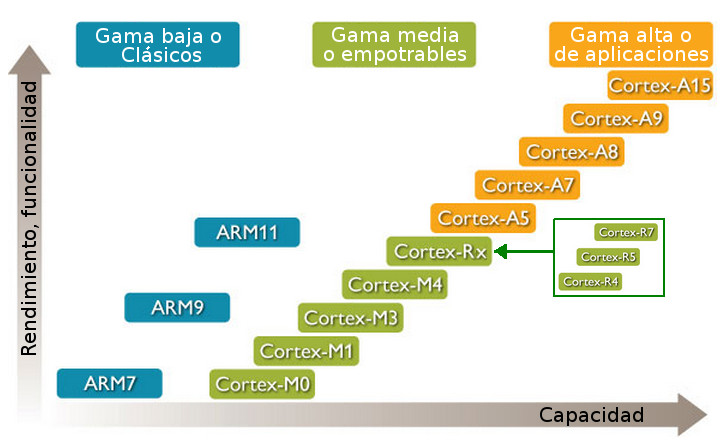
\includegraphics[width=13cm]{graphs/ArmRoadMap.jpg}
%  \caption{Clasificación de Familias ARM}
%  \label{fig:clasif_fami}
%\end{figure}

El chip en concreto que lleva la Raspberry Pi es el BCM2835, se trata de
un SoC (System on a Chip=Sistema en un sólo chip) que contiene además de
la CPU otros elementos como un núcleo GPU (hardware acelerado OpenGL
ES/OpenVG/Open EGL/OpenMAX y decodificación H.264 por hardware) y un
núcleo DSP (Digital signal processing=Procesamiento digital de señales)
que es un procesador más pequeño y simple que el principal, pero
especializado en el procesado y representación de señales analógicas.
La CPU en cuestión es la ARM1176JZF-S, un chip de la familia ARM11 que
usa la arquitectura ARMv6k. 

\begin{longtable}{| p{4.2cm} | p{2.5cm} | p{1cm} | p{6cm} |}
\hline
{\bf Familia} & {\bf Arquitectura} & {\bf Bits} & {\bf Ejemplos de dispositivos} \\ \hline
ARM1      & ARMv1       & 32/26 & Segundo procesador BBC Micro \\ \hline
ARM2, ARM3, Amber & ARMv2      & 32/26 & Acorn Archimedes \\ \hline
ARM6, ARM7 & ARMv3      & 32 & Apple Newton Serie 100 \\ \hline
ARM8, StrongARM & ARMv4       & 32 & Apple Newton serie 2x00 \\ \hline
ARM7TDMI,\newline ARM9TDMI & ARMv4T & 32 & Game Boy Advance \\ \hline
ARM7EJ, ARM9E,\newline ARM10E, XScale & ARMv5 & 32 & Samsung Omnia,\newline Blackberry 8700 \\ \hline
ARM11     & ARMv6 & 32 & iPhone 3G, Raspberry Pi \\ \hline
Cortex-M0/M0+/M1 & ARMv6-M & 32 & \\ \hline
Cortex-M3/M4 & ARMv7-M ARMv7E-M & 32 & Texas Instruments Stellaris \\ \hline
Cortex-R4/R5/R7 & ARMv7-R & 32 & Texas Instruments TMS570 \\ \hline
Cortex-A5/A7/A8/A9\newline A12/15/17, Apple A6 & ARMv7-A & 32 & Apple iPad \\ \hline
Cortex-A53/A57, X-Gene, Apple A7 & ARMv8-A & 64/32 & Apple iPhone 5S\\ \hline
\caption{Lista de familias y arquitecturas ARM}
\label{list_fam}
\end{longtable}

Las extensiones de la arquitectura ARMv6k frente a la básica ARMv6 son mínimas
\footnote{\url{http://infocenter.arm.com/help/index.jsp?topic=/com.arm.doc.ddi0301h/apbs02s02.html}}
por lo que a efectos prácticos trabajaremos con la arquitectura ARMv6.

\subsubsection{Registros}
La arquitectura ARMv6 presenta un conjunto de 17 registros (16 principales
más uno de estado) de 32 bits cada uno.
\newline

\begin{figure}[h]
  \centering
    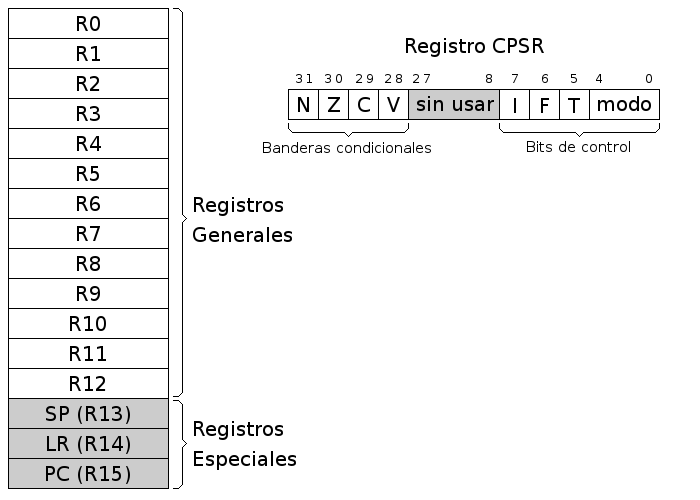
\includegraphics[width=14cm]{graphs/registros.png}
  \caption{Registros de la arquitectura ARM}
  \label{fig:reg_arm}
\end{figure}

\begin{descript}
  \item[Registros Generales.]
    Su función es el almacenamiento temporal de datos. Son los 13 registros
    que van R0 hasta R12.
  \item[Registros Especiales.]
    Son los últimos 3 registros principales: R13, R14 y R15. Como son de
    propósito especial, tienen nombres alternativos.

    \begin{itemize}
      \item{\textbf{SP}/R13. Stack Pointer ó Puntero de Pila. Sirve como puntero para almacenar
        variables locales y registros en llamadas a funciones.}
      \item{\textbf{LR}/R14. Link Register ó Registro de Enlace. Almacena la dirección de retorno
        cuando una instrucción BL ó BLX ejecuta una llamada a una rutina.}
      \item{\textbf{PC}/R15. Program Counter ó Contador de Programa. Es un registro que indica
        la posición donde está el procesador en su secuencia de instrucciones. Se
        incrementa de 4 en 4 cada vez que se ejecuta una instrucción, salvo que ésta
        provoque un salto.}
    \end{itemize}

  \item[Registro CPSR.]
        Almacena las banderas condicionales y los bits de control. Los bits de control
        definen la habilitación de interrupciones normales (I),
        interrupciones rápidas (F), modo Thumb \footnote{es un modo simplificado donde las
        instrucciones son de 16 bits en lugar de 32 y se acceden a menos registros (hasta r7),
        con la ventaja de que el código ocupa menos espacio.} (T) y el modo de operación
        de la CPU. Existen hasta 8 modos de operación, pero desde nuestra aplicación
        sólo vamos a trabajar en uno de ellos, el {\it Modo Usuario}. Los demás son modos
        privilegiados usados exclusivamente por el sistema operativo.

        Desde el {\it Modo Usuario} sólo podemos acceder a las banderas condicionales, que
        contienen información sobre el estado de la última operación realizada por la ALU.
        A diferencia de otras arquitecturas en ARMv6 podemos elegir si queremos que una
        instrucción actualice o no las banderas condicionales, poniendo una "s" detrás
        del nemotécnico \footnote{Es la forma de nombrar las instrucciones desde
        ensamblador, normalmente derivadas de una abreviatura del verbo en inglés. Por
        ejemplo la instrucción {\it MOV} viene de "move" (mover) }. Existen 4 banderas
        y son las siguientes:

    \begin{itemize}
      \item{\textbf{N}. Se activa cuando el resultado es negativo.}
      \item{\textbf{Z}. Se activa cuando el resultado es cero o una comparación es cierta.}
      \item{\textbf{C}. Indica acarreo en las operaciones aritméticas.}
      \item{\textbf{V}. Desbordamiento aritmético.}
    \end{itemize}
\end{descript}


\subsubsection{Esquema de almacenamiento}

El procesador es {\it Bi-Endian}, quiere decir que es configurable entre {\it Big Endian}
y {\it Little Endian}. Aunque nuestro sistema operativo nos lo limita a {\it Little Endian}.

Por tanto la regla que sigue es ''el byte menos significativo ocupa la posición más baja''.
Cuando escribimos un dato en una posición de memoria, dependiendo de si es byte, half word
o word,... se ubica en memoria según el esquema de la figura 1.1. La dirección de un dato
es la de su byte menos significativo. La memoria siempre se referencia a nivel de byte, es
decir si decimos la posición N nos estamos refiriendo al byte N-ésimo, aunque se escriba
media palabra, una palabra,...

***cambiar los textos del .pdf por strb r1, [r0]  strh r1, [r0]  str  r1, [r0]  
\begin{figure}[h]
  \centering
    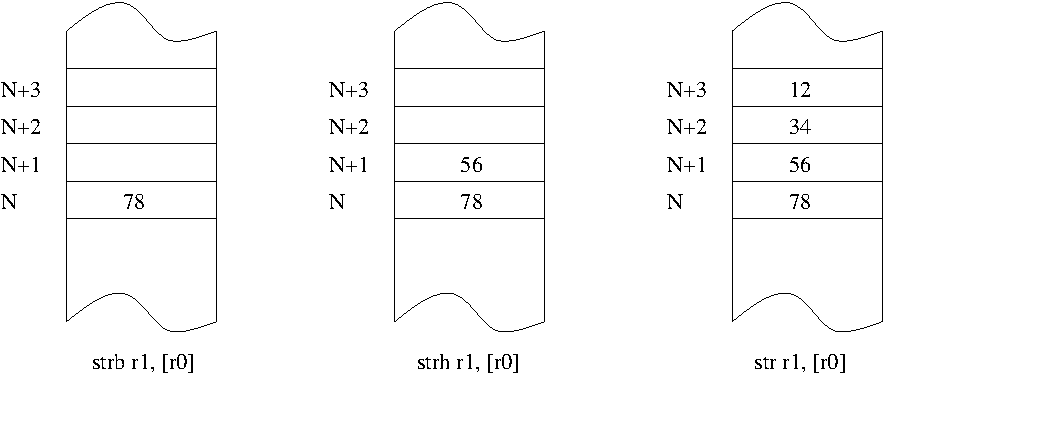
\includegraphics[width=13cm]{graphs/memo.pdf}
  \caption{Ubicación de datos en memoria}
  \label{fig:memo}
\end{figure}

\subsection{El lenguaje ensamblador}

El ensamblador es un lenguaje de bajo nivel que permite un control
directo de la CPU y todos los elementos asociados. Cada línea de un
programa ensamblador consta de una instrucción del procesador y la
posición que ocupan los datos de esa instrucción.

Desarrollar programas en lenguaje ensamblador es un proceso laborioso.
El procedimiento es similar al de cualquier lenguaje compilado.
Un conjunto de instrucciones y/o datos forman un módulo fuente.
Este módulo es la entrada del compilador, que chequea la sintaxis y lo
traduce a código máquina formando un módulo objeto.
Finalmente, un enlazador (montador ó {\it linker}) traduce todas las
referencias relativas a direcciones absolutas.

El ensamblador presenta una serie de ventajas e inconvenientes con
respecto a otros lenguajes de más alto nivel. Al ser un lenguaje de
bajo nivel, presenta como principal característica la flexibilidad y
la posibilidad de acceso directo a nivel de registro. En
contrapartida, programar en ensamblador es laborioso puesto que los
programas contienen un número elevado de líneas y la corrección y
depuración de éstos se hace difícil.

Generalmente, y dado que crear programas un poco extensos es
laborioso, el ensamblador se utiliza como apoyo a otros lenguajes
de alto nivel para 3 tipos de situaciones:
\begin{itemize}
     \item[-] Operaciones que se repitan un número elevado de veces.
     \item[-] Cuando se requiera una gran velocidad de proceso.
     \item[-] Para utilización y aprovechamiento de dispositivos y
     recursos del sistema.
\end{itemize}

\subsection{El entorno}

Los pasos habituales para hacer un programa (en cualquier lenguaje) son 
los siguientes:
lo primero es escribir el programa en el lenguaje fuente
mediante un editor de programas.
El resultado es un fichero en un lenguaje que puede entender el usuario,
pero no la máquina.
Para traducirlo a lenguaje máquina hay que utilizar un programa traductor.
Éste genera un fichero con la traducción de dicho programa, pero todavía
no es un programa ejecutable.
Un fichero ejecutable contiene el programa traducido más una serie de
códigos que debe tener todo programa que vaya a ser ejecutado en una
máquina determinada.
Entre estos códigos comunes se encuentran las librerías del lenguaje.
El encargado de unir el código del programa con el código de estas
librerías es un programa llamado montador ({\it linker}) que genera el
programa ejecutable (ver la figura \ref{fig:entorno})

***cambiar los .asm por .s
\begin{figure}[h]
  \centering
    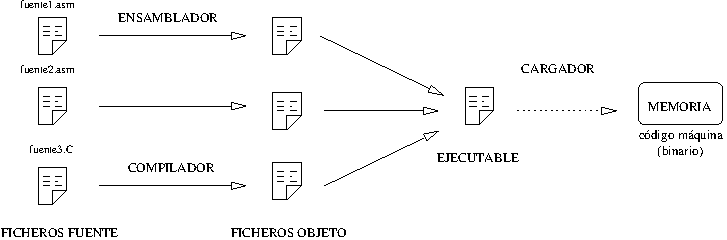
\includegraphics[width=13cm]{graphs/ensamblado.pdf}
  \caption{Entorno típico de programación}
  \label{fig:entorno}
\end{figure}

Durante el proceso de creación de un programa se suelen producir errores.
Hay dos tipos de errores: los sintácticos o detectables en tiempo de
traducción y los errores semánticos o detectables en tiempo de ejecución.
Los errores sintácticos son, por ejemplo, escribir mal una instrucción o
hacer una operación entre dos tipos de datos incompatibles.
Estos errores son detectados por el traductor y se deben solucionar para
poder generar un ejecutable.

Una vez que se tiene un programa sintácticamente correcto lo podemos
ejecutar, pero ésto no implica que el programa sea correcto. Todas las
instrucciones pueden ser correctas, pero se puede haber olvidado poner la
condición de salida de un bucle (y que no termine nunca) o que
sencillamente el programa no haga lo que queremos.

Estos errores sólo se pueden detectar en tiempo de ejecución.
Para poder eliminarlos se utiliza un depurador de programas ({\it debugger}).
El depurador nos permite ejecutar el programa instrucción a instrucción y
ver todos los valores que se van a calcular, de manera que podemos encontrar
los errores.

En el laboratorio utilizaremos el editor {\bf nano} para crear
y editar los módulos fuente de nuestros programas. El traductor
(que en el caso de traducir de un lenguaje ensamblador a lenguaje máquina
recibe el nombre de ensamblador), el {\it linker} y el {\it debugger} son
respectivamente GNU Assembler ({\bf AS}), GNU Compiler Collection ({\bf GCC})
y GNU Debbuger ({\bf GDB}). Todas estas herramientas forman parte de la
GNU toolchain que viene instalada por defecto en la mayoría de las distribuciones
basadas en Linux, en concreto Raspbian. Para obtener más información sobre estos
comandos se puede recurrir a la ayuda del sistema con <man as>, <man gcc> y
<man gdb>. Se aconseja que a lo largo de de esta
primera sesión práctica os vayais familiarizando con ambos entornos,
aunque no se os indique explícitamente.

\subsection{Aspecto de un programa en ensamblador}

En el listado \ref{lst:codigoPract1} se muestra el código de la primera
práctica que probaremos. En el código hay una serie de elementos que
aparecerán en todos los programas y que estudiaremos a continuación.

\begin{lstlisting}[caption={Código del programa intro1.s},label={lst:codigoPract1},numbers=left,escapeinside={@}{@}]
.data

var1:   .word   3
var2:   .word   4
var3:   .word   0x1234

.text
.global main
.func main
 
main:   ldr     r1, puntero_var1    /* r1 <- &var1    */
        ldr     r1, [r1]            /* r1 <- *r1      */
        ldr     r2, puntero_var2    /* r2 <- &var2    */
        ldr     r2, [r2]            /* r2 <- *r2      */
        ldr     r3, puntero_var3    /* r3 <- &var3    */
        add     r0, r1, r2          /* r0 <- r1 + r2  */
        str     r0, [r3]            /* *r3 <- r0      */
        bx      lr

puntero_var1:   .word   var1
puntero_var2:   .word   var2
puntero_var3:   .word   var3
\end{lstlisting}

La principal característica de un módulo fuente en ensamblador es
que existe una clara separación entre las instrucciones y los
datos. La {\it estructura más general de un módulo fuente} es:

\begin{description}
     \item[* Sección de datos.] Viene identificada por la directiva {\it .data}.
En esta zona se definen todas las variables que utiliza el programa
con el objeto de reservar memoria para contener los valores asignados. Hay que
tener especial cuidado para que los datos estén alineados en palabras de 4 bytes,
sobre todo después de las cadenas. Alinear significa rellenar con ceros el final
de un dato para que el siguiente dato comience en una dirección múltiplo de 4 (con
los dos bits menos significativos a cero). Los datos son modificables.

     \item[* Sección de código.] Se indica con la directiva {\it .text}, y sólo
puede contener código o datos no modificables. Como todas las instrucciones son
de 32 bits no hay que tener especial cuidado en que estén alineadas. Si tratamos
de escribir en esta zona el ensamblador nos mostrará un mensaje de error.
\end{description}

De estas tres secciones la único que obligatoriamente debe existir es
el la sección .text (o sección de código). En el ejemplo \ref{fig:codigoPract1}
comprobamos que están las dos.

Un módulo fuente, como el del ejemplo, está formado por instrucciones,
datos, símbolos y directivas. 
Las instrucciones son representaciones nemotécnicas del juego
de instrucciones del procesador. Un dato es una entidad que aporta un valor
numérico, que puede expresarse en distintas bases o incluso a través de una cadena.
Los símbolos son representaciones abstractas que el ensamblador maneja en tiempo
de ensamblado pero que en el código binario resultante tendrá un valor numérico
concreto. Hay tres tipos de símbolos: las etiquetas, las macros y las constantes simbólicas.
Por último tenemos las directivas, que sirven para indicarle ciertas cosas al
ensamblador, como delimitar secciones, insertar datos, crear macros, constantes
simbólicas, etc... Las instrucciones se aplican en tiempo de ejecución
mientras que las directivas se aplican en tiempo de ensamblado.

\subsubsection{Datos}

Los datos se pueden representar de distintas maneras. Para representar números tenemos
4 bases. La más habitual es en su forma decimal, la cual no lleva ningún delimitador
especial. Luego tenemos otra muy útil que es la representación hexadecimal, que
indicaremos con el prefijo {\it 0x}. Otra interesante es la binaria, que emplea el
prefijo {\it 0b} antes del número en binario. La cuarta y última base es la
octal, que usaremos en raras ocasiones y se especifica con el prefijo {\it 0}. Sí, un
cero a la izquierda de cualquier valor convierte en octal dicho número. Por ejemplo
015 equivale a 13 en decimal. Todas estas bases pueden ir con un signo menos delante,
codificando el valor negativo en complemento a dos. Para representar carácteres y cadenas
emplearemos las comillas simples y las comillas dobles respectivamente.

\subsubsection{Símbolos}

Como las etiquetas se pueden ubicar en tanto en la sección de datos como en la de código,
la versatilidad que nos dan las mismas es enorme. En la zona de datos pueden representar
variables, constantes y cadenas. En la zona de código etiquetas de salto, funciones y
punteros a zona de datos.

Las macros y las constantes simbólicas son símbolos cuyo ámbito pertenece al preprocesador,
a diferencia de las etiquetas que pertenecen al del ensamblador. Se especifican con las
directivas .equ y .macro respectivamente y permiten que el código sea más legible y menos
repetitivo.

\subsubsection{Instrucciones}

Las instrucciones del {\it AS} responden al formato general:


\begin{lstlisting}
Etiqueta:  Nemotécnico  Operando/s  /* Comentario */
\end{lstlisting}

De estos campos, sólo el nemónico (nombre de la instrucción) es obligatorio. En
la sintaxis del {\it AS} cada instrucción ocupa una línea terminando preferiblemente
con el ASCII 10 (LF), aunque son aceptadas las 4 combinaciones: CR, LF, CR LF y LF CR.
Los campos se separan entre sí por al menos un carácter espacio (ASCII 32) o un tabulador
y no existe distinción entre mayúsculas y minúsculas.

\begin{lstlisting}
main:   ldr     r1, puntero_var1    /* r1 <- &var1    */
\end{lstlisting}

El Campo {\it etiqueta}, si aparece, debe estar formado por una
cadena alfanumérica. La cadena no debe comenzar con un dígito y no se puede
utilizar como cadena alguna palabra reservada del {\it AS} ni nombre
de registro del microprocesador. En el ejemplo, la etiqueta es
{\tt 'main:'}.

El campo \textit{Nemotécnico} ({\tt ldr} en el ejemplo) es una forma
abreviada de nombrar la instrucción del procesador.
Está formado por caracteres alfabéticos (entre 1 y 11 caracteres).

El campo \textit{Operando/s} indica dónde se encuentran los datos.
Puede haber 0, 1 ó más operandos en una instrucción. Si hay más de uno
normalmente al primero se le denomina destino (salvo excepciones como {\tt str})
y a los demás fuentes, y deben ir separados por una coma.
Los operandos pueden ser registros, etiquetas, valores inmediatos o incluso
elementos más complejos como desplazadores/rotadores o indicadores de
pre/post-incrementos. En cualquiera de los casos el tamaño debe ser una
palabra (32 bits), salvo contadas excepciones como {\tt ldr} y {\tt str}
donde puede ser media palabra (16 bits) o un byte (8 bits).
En el ejemplo {\tt r1} es el operando destino, de tipo registro,
y {\tt puntero_var1} es el operando fuente, una etiqueta, ambos
de tamaño palabra (32 bits).

El campo \textit{Comentario} es opcional ({\tt r1 <- &var1}, en el ejemplo)
y debe comenzar con la secuencia {\tt /*} y acabar con {\tt */} al igual
que los comentarios multilínea en C. No es obligatorio que estén a la
derecha de las instrucciones, aunque es lo habitual. También es común
verlos al comienzo de una función (ocupando varias líneas) para explicar
los parámetros y funcionalidad de la misma.

Cada instrucción del {\it AS} se refiere a una operación que puede
realizar el microprocesador. También hay pseudoinstrucciones que son
tratadas por el preprocesador como si fueran macros y codifican otras
instrucciones, como {\tt lsl rn, #x} que codifica {\tt mov rn, rn, lsl #x}
o {\tt push/pop} que se traducen instrucciones {\tt stm/ldm} más complejas
y difíciles de recordar para el programador. Podemos agrupar el conjunto de
instrucciones del {\it AS}, según el tipo de función que realice el
microprocesador, en las siguientes categorías:

\begin{itemize}

       \item \textit{Instrucciones de transferencia de datos}
Mueven información entre registros y posiciones de memoria. En la
arquitectura ARMv6 no existen puertos ya que la E/S está mapeada
en memoria. Pertenecen a este grupo las siguientes instrucciones:
\textbf{mov, ldr, str, ldm, stm, push, pop}.

       \item \textit{Instrucciones aritméticas.}  Realizan operaciones
aritméticas sobre números binarios o BCD.  Son instrucciones de este
grupo \textbf{add, cmp, adc, sbc, mul}.

     \item \textit{Instrucciones de manejo de bits.}  Realizan
operaciones de desplazamiento, rotación y lógicas sobre registros o
posiciones de memoria. Están en este grupo las instrucciones:\textbf{
and, tst, eor, orr, lsl, lsr, asr, ror, rrx}.

     \item \textit{Instrucciones de transferencia de control.}  Se
utilizan para controlar el flujo de ejecución de las instrucciones
del programa. Tales como \textbf{b, bl, bx, blx} y sus variantes
condicionales.

\end{itemize}

En esta sesión práctica se explorarán algunas de estas instrucciones.
Para buscar información sobre cualquiera de ellas durante las prácticas,
recuerda que puedes utilizar el datasheet del ARM1176JZF-S.

\chapterend{}

%%%%%%%%%%%%%%%%%%%%%%%%%%%%%%%%%%%%%%%%%%%%%%%%%%%%%%%%%%%%%%
\end{document}

% Capítulo 02.
\documentclass[12pt,a4paper]{book} % article, report, book.
%%%%%%%%%%%%%%%%%%%%%%%%%%%%%%%%%%%%%%%%%%%%%%%%%%%%%%%%%%%%%%%%%%%
%%% Documento LaTeX                                             %%%
%%%%%%%%%%%%%%%%%%%%%%%%%%%%%%%%%%%%%%%%%%%%%%%%%%%%%%%%%%%%%%%%%%%
% Título: Paquetes
% Autor:  Ignacio Moreno Doblas
% Fecha:  2014-02-01
%%%%%%%%%%%%%%%%%%%%%%%%%%%%%%%%%%%%%%%%%%%%%%%%%%%%%%%%%%%%%%%%%%%
% Tabla de materias:
% 1 Codificación e idioma %
% 2 Matemáticas y Física %
% 3 Gráficos%
% 4 Estilo y formato%
%%%%%%%%%%%%%%%%%%%%%%%%%%%%%%%%%%%%%%%%%%%%%%%%%%%%%%%%%%%%%%%%%%%

%1 Codificación e idioma%
\usepackage[utf8]{inputenc} %Codificación en utf8%
\usepackage[spanish]{babel} %Hyphenation (Guionado) en español%
\usepackage[T1]{fontenc} %Codificación de fuente%
\usepackage{eurofont} %Tipografía euro (€)%

%2 Matemáticas y Física %
% Importante para ecuaciones, magnitudes y unidades%
\usepackage{amssymb,amsmath,latexsym,amsfonts} % paquetes estándar%
\usepackage[squaren]{SIunits} %Paquete para magnitudes y unidades físicas%
\usepackage{ifthen} %sentencias if y while%

%3 Gráficos%
\usepackage{graphics,graphicx} %paquetes gráficos estándar%
\usepackage{wrapfig} %paquete para gráfica lateral%
\usepackage[rflt]{floatflt} %figuras flotantes%
  % \begin{floatingfigure}[r]/[l]{4.5cm}
  % \end{floatingfigure}
\usepackage{graphpap} %comando \graphpaper en el entorno picture%

%4 Estilo y formato%
\usepackage{fancyhdr} %cabeceras y pies mejor que con \pagestyle{}%
\usepackage{titlesec,titletoc} %Formateo de secciones y títulos%
\raggedbottom %Para fragmentar versos en varias páginas%
\usepackage{makeidx} %MakeIndex%
%\usepackage{showidx} % Hace que cada comando \index se imprima en la página donde se ha puesto (útil para corregir los índices)
\usepackage{alltt} % Define el environment alltt, como verbatim, excepto que \, { y } tienen su significado normal. Se describe en el fichero alltt.dtx.
\usepackage[pdftex,bookmarksnumbered,hidelinks]{hyperref} %hyper-references%
\usepackage{minitoc} % Para poner tablas de contenido en cada capítulo.
\usepackage{listings} % Para escribir piezas de código C, Python, etc. %
%listings configuration
\lstset{
  language=[ARM]Assembler, %Puede ser C, C++, Java, etc.
  showstringspaces=false,
  formfeed=\newpage,
  tabsize=4,
  commentstyle=\itshape,
  basicstyle=\ttfamily,
  morekeywords={models, lambda, forms}
}

\usepackage{tipa} % tipografía IPA (International Phonetic Alphabet)
\usepackage{longtable} %Entorno Longtable, fracciona tablas a lo largo de páginas%
\usepackage{colortbl}
\usepackage{acronym}  %Para expandir automáticamente los acrónimos

%%%%%%%%%%%%%%%%%%%%%%%%%%%%%%%%%%%%%%%%%%%%%%%%%%%%%%%%%%%%%%%%%%%
% Tabla de materias:
% 1 Información del Documento %
% 2 Comandos a nivel de texto %
% 3 Comandos a nivel de entorno %
% 4 Comandos a nivel de página y sección %
% 5 Otros comandos %
%%%%%%%%%%%%%%%%%%%%%%%%%%%%%%%%%%%%%%%%%%%%%%%%%%%%%%%%%%%%%%%%%%%

% 1 Información del Documento %
\newcommand{\pfctitlename}{Guiones de prácticas sobre la plataforma Raspberry Pi}
\newcommand{\pfcauthorname}{Antonio José Villena Godoy}
\newcommand{\pfctutorname}{Rafael Asenjo Plaza \\ Francisco Javier Corbera Peña}
\newcommand{\pfcanno}{2015}

% 2 Comandos a nivel de texto %
\newcommand{\R}{\textsuperscript{\textregistered}}  %Símbolo registrado%
\newcommand{\C}{\textsuperscript{\copyright}} %Símbolo Copyright%
\newcommand{\TM}{\texttrademark} %Símbolo Trade Mark (marca comercial)%

% 2.1 Comandos abreviatura %
\newcommand{\tit}{\textit} %Fuente cursiva (itálica)%
\newcommand{\tbf}{\textbf} %Fuente negrita%
\newcommand{\ttw}[1]{\texttt{#1}} %Fuente máquina de escribir (typewriter)%
%Combinación%
\newcommand{\textittt}[1]{\textit{\texttt{#1}}} %itálica y typewriter%
\newcommand{\textittw}{\textittt} % Otra forma de escribirlo.
\newcommand{\tittw}{\textittw} %Shortened%
\newcommand{\tbftw}[1]{\tbf{\ttw{#1}}}

%Crea una nueva línea y la indenta sin crear interlineado extra.
\newcommand{\nli}{\\ \indent} 

%Para escribir un correo electrónico%
\newcommand{\mailto}[1]{\href{mailto:#1}{#1}}

% Si vas a hacer un uso básico de \index (entradas en el índice de sólo un nivel, sin formatos especiales, etc.), define la orden
\newcommand{\miindex}[1]{#1\index{#1}}

\newcommand{\hs}{\hspace} % Abreviatura espacio horizontal
\newcommand{\vs}{\vspace} % Abreviatura espacio vertical

% Abreviaturas para los conjuntos de números más comunes.
\newcommand{\realnumbers}{\mathbb R}
\newcommand{\naturalnumbers}{\mathbb N}
\newcommand{\integernumbers}{\mathbb Z}
\newcommand{\rationalnumbers}{\mathbb Q}
\newcommand{\complexnumbers}{\mathbb R}
\newcommand{\irrationalnumbers}{\mathbb I}

% Doble barra sobre una letra (para expresar las matrices).
\newcommand{\doublebar}[1]{\bar{\bar{#1}}} 
% Ej: \vector(y) = \doublebar(A) \vector(x) (Stma. lineal de ec.)

% 3 Comandos a nivel de entorno %
\newcommand{\benu}{\begin{enu}} % Begin enumerate
\newcommand{\eenu}{\end{enu}}   % End enumeration

%Comando para escribir código Python
\newcommand{\code}[3]{
  %\hrulefill
  %\subsection*{#1}
  %\subsubsection{#1}
  \lstinputlisting{#2}
  %#1\\
  \begin{table}[h!]
    \centering
    \caption{#1}
    \label{#3}
  \end{table}
  \vspace{2em}
}

% 4 Comandos a nivel de página y sección %
%Crea página en blanco
\newcommand{\blankpage}{\clearpage{\pagestyle{empty}\cleardoublepage}}

% Versión x del comando section: sin numeración pero sí aparece en la tabla de contenidos.
\newcommand{\sectionx}[1]{
  \section*{#1}
  \addcontentsline{toc}{section}{#1}
}

% Versión y del comando section: sin numeración y NO aparece en la tabla de contenidos.
\newcommand{\sectiony}[1]{
  \section*{#1}
}

% Versión x del comando chapter: sin numeración pero sí  aparece en la tabla de contenidos.
\newcommand{\chapterx}[1]{
  \chapter*{#1}
  %\addcontentsline{toc}{chapter}{#1} %Caused by minitoc package%
  \addstarredchapter{#1} %For minitoc package%
}

% substituto del comando \chapter: incluye estilo de página.
\newcommand{\chapterbegin}[1]%
  {%
    \pagestyle{fancy}
    \fancyhead[LE,RO]{\thepage}
    \fancyhead[LO]{Capítulo \thechapter. #1}
    %\fancyhead[RE]{Parte \thepart \rightmark} %
    \fancyhead[RE]{\nouppercase{\rightmark}} %
        
    \chapter{#1}
  }

% Versión x del comando \chapterbegin: sin numeración y aparece en la tabla de contenidos.
\newcommand{\chapterbeginx}[1]%
  {%
    \pagestyle{fancy}
    \fancyhead[RO,LE]{\thepage}
    \fancyhead[RE,LO]{#1}
    %\fancyhead[LO]{Chapter \thechapter}
    %\fancyhead[RE]{Part \thepart} %
    
    \chapterx{#1}
  }

%Fin de capítulo
\newcommand{\chapterend}{\pagestyle{empty}\cleardoublepage \thispagestyle{empty}}
%Si fuera un artículo en lugar un libro, \clearpage en lugar de \cleardoublepage

% 5 Otros comandos %
%\let\Oldpart\part
%\newcommand{\parttitle}{}
%\renewcommand{part}[1]{\Oldpart{#1}\renewcommand{\parttitle}{#1}} %Header customization%

%Cambiar el título índice de capítulo a ``Contenido''.
\renewcommand{\mtctitle}{Contenido}

\dominitoc % Para tablas de contenidos por capítulo.

\addto{\captionsspanish}{
  \renewcommand{\listtablename}{Índice de Tablas}
  \renewcommand{\tablename}{Tabla} } % Por ejemplo, modificar el nombre de 'Cuadro' a 'Tabla'.

\addto{\captionsspanish}{
  \renewcommand{\contentsname}{Índice} }

%Si se desea cambiar el tipo de letra a Arial
% por cualquier razón, descomentar las siguientes
% dos líneas
%\renewcommand{\rmdefault}{phv} % Arial
%\renewcommand{\sfdefault}{phv} % Arial
  
%\addto{\captionsspanish}{
% \renewcommand{\partname}{Fase} }

%\addto{\captionsspanish}{%
%    \renewcommand{\refname}{\vspace{-4.5ex}}} % Para que no aparezca el texto 'referencias' en la bibliografía.

% Modifica el interlineado
%\renewcommand{\baselinestretch}{1.5}

   \definecolor{myfboxbg}{gray}{0.9}
   \newsavebox{\efcaja}
   \newenvironment{myfbox}{\begin{lrbox}{\efcaja}}
               {\end{lrbox}{\colorbox{myfboxbg}{\usebox{\efcaja}}}}

%%%%%%%%%%%%%%%%%%%%%%%%%%%%%%%%%%%%%%%%%%%%%%%%%%%%%%%%%%%%%%%%%%%
% Tabla de materias:
%--------------------%
% 1 dobleindent
% 2 izqindent
% 3 dobleindentx
% 4 ite
% 5 descript
% 6 enu
% 7 itemization
% 8 sinopsis
% 9 objetivo
%%%%%%%%%%%%%%%%%%%%%%%
% Para conocer los parámetros de diseño de las listas, tales como
%  los márgenes izquierdo, derechos y los diferentes saltos,
%  véase el archivo ``List layout.png'' que acompaña esta plantilla.
% Así se conocerá mejor cómo adaptar un entorno según los requisitos 
%  del usuario.

%%%%%%%%%%%%%%%%%%%%%%%
% Definición de longitudes para usar en los entornos:
%
% Normal parskip.
\newlength{\parskipenv}
\setlength{\parskipenv}{\parskip}

\newlength{\parindentenv}
\setlength{\parindentenv}{\parindent}
%%%%%%%%%%%%%%%%%%%%%%%

% 1 dobleindent
%El entorno dobleindent está pensando para escribir párrafos con doble indentación a cada lado.
%Tiene dos parámetros de entrada con las distancias medidas desde los márgenes de página.

\newenvironment{dobleindent}[2]
  %Comienzo de nuevo entorno%
  {
  \begin{list}
    {}
    {
    % Left and right margins:
    \leftmargin = #1 
    \rightmargin = #2
    %
    % Separation from preceding and following text:
    \topsep = 0ex
    \partopsep = 0ex
    \parsep = \parskipenv
    %
    % Indentation for paragraphs:
    \itemsep = \parskipenv
    \itemindent = \parindentenv
    \listparindent = \itemindent
    %
    % Horizontal separation from label:
    \labelsep = 1ex
    \settowidth{\labelwidth}{0cm}
    }
    
     \item}
  % End new env
  {\end{list}}

%%%%%%%%%%%%%%%%%%%%%%%%%%%%%
%2 izqindent
% El entorno izqindent sólo crea un párrafo indentado a la izquierda.
\newenvironment{izqindent}[1]
{
\begin{dobleindent}{#1}{0cm}
}
{
\end{dobleindent}
}

%%%%%%%%%%%%%%%%%%%%%%%%%%%%%
% 3 dobleindentx
% El entorno dobleindentx es una variación del dobleindent usando leftskip y rightskip.
% Aunque es más limitado, también se puede usar.
\newenvironment{dobleindentx}[2] % Sólo funciona en modo paragraph
{ % Preamble
  \leftskip = #1
  \rightskip = #2
}
{ % Postamble
\leftskip = 0cm
\rightskip = 0cm
}

%%%%%%%%%%%%%%%%%%%%%%%%%%%%%
% 4 ite
% El entorno ite es una modificación del entorno itemize estándar de \LaTeX. Puede usarse o modificarse si el usuario lo desea.
% También puede parametrizarse el entorno enumerate o description de forma equivalente.
\newenvironment{ite}
  {
    \begin{izqindent}{\parindent}
    \hspace{-\parindent}  % compensación del sangrado que introduce el entorno.
    \vspace{-1.0\parskip} % compensación del \parskip que introduce el entorno.
    \vspace{-\baselineskip} % compensación por la línea que introduce el entorno.
    \begin{itemize}
  }
  {
    \end{itemize}
    \end{izqindent}
  }

%%%%%%%%%%%%%%%%%%%%%5
% commando stdformat para formatear los entornos descript, enu y itemization.
\newcommand{\stdformat}
  {% Declarations for format presentation.
    %     
    % Separation from preceding and following text:
    \setlength{\topsep}{0ex}%
    \setlength{\partopsep}{0ex} %
    %
    % Horizontal separation from label:
    \labelsep = 1ex
    \setlength{\labelwidth}{0ex}
    %
    % Left and right margins: 
    \setlength{\leftmargin}{1cm}%
    \addtolength{\leftmargin}{\labelsep}
    \setlength{\rightmargin}{0ex}
    %  
    % Indentation for paragraphs:
    \setlength{\itemindent}{-\leftmargin}%
    \addtolength{\itemindent}{1ex}
    \setlength{\listparindent}{\parindent}%
    %   
    % Separation between paragraphs.
    \setlength{\parsep}{\parskipenv}% 
    \setlength{\itemsep}{1ex}
  }

%%%%%%%%%%%%%%%%%%%%%%%%%%%%%
% 5 descript

\newenvironment{descript}
  % Beginning new env def.
  {
    \begin{list}
      {} % No default label for \item.
      {
        % Declarations for format presentation.
        \stdformat
        %
        \renewcommand{\makelabel}[1]{\normalfont\bfseries##1\hfil}
      }
  }
  % Ending new env def.
  {
    \hspace*{\fill} \\ \end{list}
  } % Se introduce un salto de línea para que el texto siguiente esté separado.
%END newenvironment{descript}

%%%%%%%%%%%%%%%%%%%%%%%%%%%%%
% 6 enu
\newcounter{itemnumber} % Counter for the environment.

\newenvironment{enu}
  % Beginning new env def.
  {
    \begin{list}
    {
      \raggedleft \arabic{itemnumber}
    }
    {
      \usecounter{itemnumber}
      \stdformat
    }
  }
  {
    \end{list}
  }

%%%%%%%%%%%%%%%%%%%%%%%%%%%%%
% 7 itemization
\newenvironment{itemization}
  % Beginning new env def.
  {
    \begin{list}
      {$\bullet$} % No default label for \item.
      {
        % Declarations for format presentation.
        \stdformat
      }
  }
  % Ending new env def.
  {
    \end{list}
  }


%%%%%%%%%%%%%%%%%%%%%%%%%%%%%
% 8 sinopsis
\newenvironment{sinopsis}{%[1]{
  \sectiony{Sinopsis}
  %\label{#1}
} {
  \pagebreak
}

%%%%%%%%%%%%%%%%%%%%%%%%%%%%%
% 9 objetivo
\newenvironment{objetivo}{%[1]{
  \sectiony{Objetivo}
  %\label{#1}
} {
}

%%%%%%%%%%%%%%%%%%%%%%%%%%%%%%%%%%%%%%%%%%%%%%%%%%%%%%%%%%%%%%%%%%%
% Tabla de materias:
%--------------------%
% 1 Márgenes de página
%%%%%%%%%%%%%%%%%%%%%%%
% Para conocer los parámetros de diseño de páginas, tales como
%  los márgenes izquierdo, derecho, anchura de página, etc.
%  véase el archivo ``Page layout.png'' que acompaña esta plantilla.
% Así se conocerá mejor cómo adaptar el documento según los 
%  requisitos del usuario.

% 1 Márgenes de página
%-------------------------------%
% Parámetros de estilo de página.
% DIN A4: 29.7 cm x 21 cm
%   área neta: 3 cm + 3 cm + 15 cm.
%
% Definición de márgenes de página
%  even para páginas pares
%  odd  para páginas impares
\newlength{\realoddsidemargin}    % \oddsidemargin menos 1 in.
\newlength{\realevensidemargin}   % \evensidemargin menos 1 in.
\newlength{\realtopmargin}        % \topmargin menos 1 in.
%
% Asignación de márgenes de página
% ASIGNESE en caso de querer cambiarlo
\setlength{\realtopmargin}{2cm}     % REAL top margin.
\setlength{\realoddsidemargin}{3cm}   % REAL oddside margin.
\setlength{\realevensidemargin}{3cm}  % REAL evenside margin.
\setlength{\hoffset}{0cm}
\setlength{\voffset}{0cm}
%
% Substracción de 1 pulgada de compensación
%  (véase ``Page Layout.png'' para más información)
\addtolength{\realoddsidemargin}{-1in}  % 1 inch = 2.54 cm.
\addtolength{\realevensidemargin}{-1in}
\addtolength{\realtopmargin}{-1in}
%
% Asignación de anchuras y márgenes
% No hay notas al margen
\setlength{\marginparsep}{0cm} % No van a existir notas al margen
\setlength{\marginparwidth}{0cm} % No van a existir notas al margen
%
% Asignación de anchura de texto
\setlength{\textwidth}{15cm}  % Anchura neta del texto (globalmente).
%
% Asignación de márgenes par, impar y en altura
\setlength{\oddsidemargin}{\realoddsidemargin}  % odd-page left margin (global).
\setlength{\evensidemargin}{\realoddsidemargin} % even-page left margin (global).
\setlength{\topmargin}{\realtopmargin}          % top margin (Global).

% Se puede usar también el paquete chngpage.

%%%%%%%%%%%%%%%%%%%%%%%%%%%%%%%%%%%%%%%%%%%%%%%%%%%%%%%%%%%%%%%%%%
%   1 Length commands.          %
%-------------------------------%
% Defines new length command (e.g., \newlength{\gnat}}
% \newlength{}
%
% Set lenght to a value.
% \setlength{\gnat}{length}
% \addtolength{}{}
%
% Sets the value of a length command equal to the width of a specified piece of text; e.g., \settowidth{\parindent}{\em small}.
% \settowidth{}{}
% Set the value of a height. e.g., \settoheight{\parskip}{Gnu}
% \settoheight{}{}
% Set the value that extends below the line. e.g., \settodepth{\parskip}{gnu}.
% \settodepth{}{}
%
% To multiply a length, write: 7.0\gnat = \gnat * 7.0
%%%%%%%%%%%%%%%%%%%%%%%%%%%%%%%%%%%%%%%%%%%%%%%%%%%%%%%%%%%%%%%%%%

\begin{document}

%%%%%%%%%%%%%%%%%%%%%%%%%%%%%%%%%%%%%%%%%%%%%%%%%%%%%%%%%%%%%%

\chapterbegin{Tipos de datos y sentencias de alto nivel}
\label{chp:TipDat}
\minitoc

{\bf Objetivo}:
En esta sesión repasaremos cómo se representa la
información en la memoria del computador: veremos la definición en
ensamblador de punteros, vectores y matrices. También veremos cómo se programan las
estructuras de alto nivel del tipo {\tt if-else} y los bucles {\tt
for} y {\tt while}.

\section{Lectura previa}

\subsection{Modos de direccionamiento del ARM}

En la arquitectura ARM los accesos a memoria se hacen mediante instrucciones
específicas {\tt ldr} y {\tt str} (luego veremos las variantes {\tt ldm},
{\tt stm} y las preprocesadas {\tt push} y {\tt pop}). El resto de instrucciones
toman operandos desde registros o valores inmediatos, sin excepciones. En este
caso la arquitectura nos fuerza a que trabajemos de un modo determinado: primero
cargamos los registros desde memoria, luego procesamos el valor de estos registros
con el amplio abanico de instrucciones del ARM, para finalmente volcar los
resultados desde registros a memoria. Existen otras arquitecturas como la Intel x86,
donde las instrucciones de procesado nos permiten leer o escribir directamente
de memoria. Ningún método es mejor que otro, todo es cuestión de diseño. Normalmente
se opta por direccionamiento a memoria en instrucciones de procesado en arquitecturas
con un número reducido de registros, donde se emplea la memoria como almacén
temporal. En nuestro caso disponemos de suficientes registros, por lo que podemos
hacer el procesamiento sin necesidad de interactuar con la memoria, lo que por otro
lado también es más rápido.

\begin{descript}
  \item[Direccionamiento inmediato.]
    El operando fuente es una constante, formando parte de la instrucción.
\begin{lstlisting}
    mov     r0, #1
    add     r2, r3, #4
\end{lstlisting}
  \item[Direccionamiento inmediato con desplazamiento o rotación.]
    Es una variante del anterior en la cual se permiten operaciones intermedias
    sobre los registros.
\begin{lstlisting}
    mov     r1, r2, LSL #1      /* r1 <- (r2*2) */
    mov     r1, r2, LSL #2      /* r1 <- (r2*4) */
    mov     r1, r3, ASR #3      /* r1 <- (r3/8) */
\end{lstlisting}
    Implicitamente también interviene en la creación de constantes, rotando o
    desplazando constantes más pequeñas de forma transparente al usuario. Como todas
    las instrucciones ocupan 32 bits, es técnicamente imposible que podamos cargar
    en un registro cualquier constante de 32 bits con la instrucción {\tt mov}. Por
    esta razón cuando se necesita cargar una constante más compleja en un registro
    (como una dirección a una variable de memoria) no podemos hacerlo con la instrucción
    {\tt mov}, tenemos que recurrir a {\tt ldr} con direccionamiento a memoria. En algunos
    casos es difícil determinar si el ensamblador conseguirá codificar una constante
    por medio de esta técnica, con lo que la única solución es probar.
\begin{lstlisting}
    mov     r1, #0x80000020
\end{lstlisting}
    Ensamblamos y vemos que no da problemas. Sin embargo con esta otra.
\begin{lstlisting}
    mov     r1, #0x80000040
\end{lstlisting}
    El ensamblador nos muestra el siguiente error.
\begin{lstlisting}
intro1.s: Assembler messages:
intro1.s:10: Error: invalid constant (80000040) after fixup
\end{lstlisting}

  \item[Direccionamiento a memoria, sin actualizar registro puntero.]
    Es la forma más sencilla y admite 4 variantes. Después del acceso
    a memoria ningún registro implicado en el cálculo de la dirección
    se modifica.
\begin{itemize}
  \item{\tt [Rx, \#+inmediato] \newline
            [Rx, \#-inmediato] \newline}
    Simplemente añade (o sustrae) un valor inmediato al registro dado
    para calcular la dirección. Es muy útil para acceder a elementos
    fijos de un array, ya que el desplazamiento es constante. Por
    ejemplo si tenemos {\tt r1} apuntando a un array de enteros de
    32 bits {\tt int a[]} y queremos poner a 1 el
    elemento {\tt a[3]}, lo hacemos así.

\begin{lstlisting}
    mov     r2, #1          /* r2 <- 1          */
    str     r2, [r1, #+12]  /* *(r1 + 12) <- r2 */
\end{lstlisting}

    Nótese que hemos multiplicado por 4 el desplazamiento porque cada
    elemento del array son 4 bytes. El desplazamiento no puede ser mayor
    de 12 bits, por lo que nuestro rango está límitado entre {\tt [Rx, \#-4095]}
    y {\tt [Rx, \#+4095]}.

  \item{\tt [Rx, +Ry] \newline
            [Rx, -Ry] \newline}

    Parecido al anterior pero en lugar de un inmediato emplea otro registro. Útil
    en el caso de queramos mantener fijo el registro {\tt Rx} y movernos con {\tt Ry},
    o bien para acceder a desplazamientos mayores a 4095. El mismo ejemplo de
    arriba utilizando esta variante sería.

\begin{lstlisting}
    mov     r2, #1          /* r2 <- 1          */
    mov     r3, #12         /* r3 <- 12         */
    str     r2, [r1, +r3]   /* *(r1 + r3) <- r2 */
\end{lstlisting}

  \item{\tt [Rx, +Ry, operación\_desp \#inmediato] \newline
            [Rx, -Ry, operación\_desp \#inmediato] \newline}

    En este caso aplicamos una operación de desplazamiento
    o rotación sobre el segundo registro {\tt Ry}. Muy útil
    en caso de arrays o estructuras con elementos de longitud
    potencia de 2, ya que podemos indexar directamente. El
    mismo ejemplo de antes.
    
\begin{lstlisting}
    mov     r2, #1
    mov     r3, #3
    str     r2, [r1, +r3, LSL #2]
\end{lstlisting}

    Nótese cómo accedemos a {\tt a[3]}
    directamente con el valor del índice, {\tt 3}).
\end{itemize}


  \item[Direccionamiento a memoria, actualizando registro puntero.]
    En este modo de direccionamiento, el registro que genera la dirección
    se actualiza con la propia dirección. De esta forma podemos recorrer
    un array con un sólo registro sin necesidad de hacer el incremento del
    puntero en una instrucción aparte. Hay dos métodos de actualizar dicho
    registro, antes de ejecutar la instrucción (preindexado) o después
    de la misma (postindexado). Los tres siguientes tipos son los
    postindexados.

\begin{itemize}
  \item{\tt [Rx], \#+inmediato \newline
            [Rx], \#-inmediato \newline}
    Una notación muy parecida a la versión que no actualiza registro, la única
    diferencia es que la constante de desplazamiento queda fuera de los corchetes.
    Presenta el mismo límite de hasta 4095. Este ejemplo pone a cero los 3 primeros
    elementos {\tt a[0], a[1], a[2]} del array.

\begin{lstlisting}
    mov     r2, #0          /* r2 <- 0      */
    str     r2, [r1], #+4   /* a[0] <- r2   */
    str     r2, [r1], #+4   /* a[1] <- r2   */
    str     r2, [r1], #+4   /* a[2] <- r2   */
\end{lstlisting}

  \item{\tt [Rx], +Ry \newline
            [Rx], -Ry \newline}
    Igual que antes pero con registro en lugar de inmediato.

  \item{\tt [Rx], +Ry, operación\_desp \#inmediato \newline
            [Rx], -Ry, operación\_desp \#inmediato \newline}

    Nótese que en todos los modos postindexados
    encerramos entre llaves el primer registro, que es el que se va
    a utilizar en la instrucción de lectura o escritura en memoria. Es decir
    primero cargamos de {\tt [Rx]} y luego actualizamos {\tt Rx} con el valor
    que corresponda. Esta instrucción.

\begin{lstlisting}
    ldr     r2, [r1], +r3, LSL #2
\end{lstlisting}

    Se puede desglosar en estas otras dos, cuyo comportamiento es exactamente
    el mismo.

\begin{lstlisting}
    ldr     r2, [r1]
    add     r1, r1, r3, LSL #2
\end{lstlisting}
\end{itemize}

    Ya hemos visto la notación postindexada. Veamos ahora los tres modos
    preindexados.

\begin{itemize}
  \item{\tt [Rx, \#+inmediato]! \newline
            [Rx, \#-inmediato]! \newline}
    La idea en todos los casos es encerrar entre corchetes la dirección que
    se va a usar en la instrucción. Para diferenciarlo del caso que no actualiza
    el registro le añadimos un {\tt !} al final.

    Este modo es muy útil en casos que queramos reusar en una futura instrucción
    la dirección que hemos calculado. En este ejemplo duplicamos el valor
    que se encuentra en {\tt a[3]}.

\begin{lstlisting}
    ldr     r2, [r1, #+12]!
    add     r2, r2, r2
    str     r2, [r1]
\end{lstlisting}

  \item{\tt [Rx, +Ry]! \newline
            [Rx, -Ry]! \newline}

    Similar al anterior pero usando {\tt Ry} en lugar de inmediato.

  \item{\tt [Rx, +Ry, operación\_desp \#inmediato]! \newline
            [Rx, -Ry, operación\_desp \#inmediato]! \newline}

    Tercer y último caso de direccionamiento preindexado. Al igual que
    antes, desgloso en dos instrucciones para ver el funcionamiento exacto.

\begin{lstlisting}
    ldr     r2, [r1, +r3, LSL #2]!
\end{lstlisting}

    Equivale a esto.

\begin{lstlisting}
    ldr     r2, [r1, +r3, LSL #2]
    add     r1, r1, r3, LSL #2
\end{lstlisting}

    O bien a esto otro.

\begin{lstlisting}
    add     r1, r1, r3, LSL #2
    ldr     r2, [r1]
\end{lstlisting}
\end{itemize}


\subsection{Tipos de datos}

\vspace{0.25cm}
{\bf Tipos de datos básicos.} En la siguiente tabla se recogen los diferentes tipos de datos básicos
 que podrán aparecer en los ejemplos, así como su tamaño y  rango de
representación.

\vspace{1cm}
\begin{center}
%\begin{table}[h!]
\begin{tabular}{|l|l|c|c|}\hline
 ARM & Tipo en C & bits & Rango \\ \hline
 {\tt .byte}  & {\tt unsigned char} & 8 & 0 a 255 \\
              & ({\tt signed}) {\tt char} & 8 & -128 a 127 \\ \hline
 {\tt .hword} & {\tt unsigned short int} & 16 &  0 a 65.535 \\
 {\tt .short} & ({\tt signed}) {\tt short int} & 16 & -32.768 a 32767 \\ \hline
 {\tt .word}  & {\tt unsigned int} & 32 & 0 a 65.535 \\
 {\tt .int}   & ({\tt signed}) {\tt int} &  32 & -32.768 a 32.767 \\
              & {\tt unsigned long int}  & 32 & 0 a 4294967296 \\ 
              & ({\tt signed}) {\tt long int} &  32 & -2147483648 a 2147483647 \\ \hline
 {\tt .quad}  & {\tt unsigned long long} & 64 &  0 a $2^{64}$ \\
              & ({\tt signed}) {\tt long long} & 64 & -$2^{63}$ a $2^{63}$-1 \\ \hline
\end{tabular}
%\end{table}
\end{center}

Nótese como en ensamblador los tipos son neutrales al signo, lo importante
es la longitud en bits del tipo. La mayoría de las instrucciones (salvo
multiplicación) hacen la misma operación tanto si se trata de un número
natural como si es entero en complemento a dos. Nosotros decidiremos el tipo
mediante las constantes que pongamos o según los flags que interpretemos del
resultado de la operación.
\end{descript}


\noindent{\bf Punteros.} Un {\bf puntero} siempre ocupa 32 bits y contiene
una dirección de memoria. En ensamblador no tienen tanta utilidad como en C,
ya que disponemos de registros de sobra y es más costoso acceder a
las variables a través de los punteros que directamente. En este ejemplo
acceder a la dirección de var1 nos cuesta 2 {\tt ldrs} a través del puntero,
mientras que directamente se puede hacer con uno sólo.


\begin{lstlisting}
.data
var1:           .word   3
puntero_var1:   .word   var1

.text
.global main
main:   ldr     r0, =puntero_var1
        ldr     r1, [r0]
        ldr     r2, [r1]
        ldr     r3, =var1
        bx      lr
\end{lstlisting}

Observamos cómo el valor de {\tt r3} es el mismo que el de {\tt r1}.

\begin{lstlisting}
(gdb) ni 4
0x000083a0 in main ()
(gdb) i r r0 r1 r2 r3
r0             0x1054c  66892
r1             0x10548  66888
r2             0x3      3
r3             0x10548  66888
\end{lstlisting}

Incluso en tipos que en C están basados en punteros como las cadenas,
en ensamblador no es necesario tenerlos almacenados en memoria puesto
que podemos obtener dicho valor en un registro con una única instrucción {\tt ldr}.

\vspace{0.25cm}
\noindent{\bf Vectores.} Todos los elementos de un vector se almacenan en un único
bloque de memoria a partir de una dirección determinada. Los
diferentes elementos se almacenan en posiciones consecutivas, de
manera que el elemento {\tt i}  está entre los {\tt i-1} e {\tt i+1}
(figura \ref{fig:dos_3}). Los
vectores están definidos siempre a partir de la posición 0. El propio
índice indica cuántos elementos hemos de desplazarnos respecto del
comienzo del primer elemento (para acceder al elemento cero hemos de
saltarnos 0 elementos, para acceder al elemento 1 hemos de saltarnos
un elemento, etc... En general, para acceder al elemento con índice
{\tt i}
hemos de saltarnos los {\tt i} elementos anteriores).

Dado un vector {\tt int v[N];}, todos los elementos se encuentran en posiciones
consecutivas a partir de la dirección de {\tt v[0]}
(puesto que son {\tt int}, en este ejemplo, cada elemento ocupa 4 bytes). Por lo tanto,
el acceso al elemento {\tt v[i]} se consigue aplicando la siguiente expresión.

\begin{equation}
v[i] = M_d[@v[0] + i*4] 
\label{eq:uno}
\end{equation}

Con $ @v[0]$ nos referimos a la dirección en memoria del elemento
 $ v[0]$. Con $ M_d[\ ]$ notamos el acceso a memoria para la lectura/escritura
de un dato (el número de bytes de memoria implicado dependerá del tipo
de datos declarado). Cuando nos queramos refererir al acceso a memoria
para la obtención de un puntero, lo notaremos como
$ M_{ref}[\ ]$.

\begin{figure}[h]
  \centering
    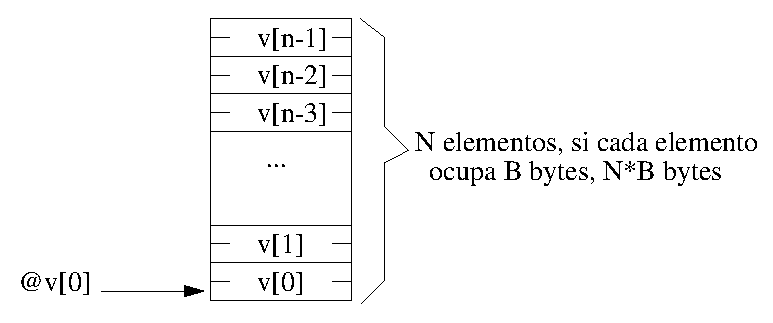
\includegraphics[width=10cm]{graphs/2-3.eps}
  \caption{Representación de un vector en memoria}
  \label{fig:dos_3}
\end{figure}


\noindent{\bf Matrices bidimensionales.} Una matriz bidimensional de N$\times$M
elementos se almacena en un único bloque de memoria. Interpretaremos
una matriz de N$\times$M como una matriz con $N$ filas de $M$ elementos cada
una. Si cada elemento de la matriz ocupa $B$ bytes, la matriz ocupará un
bloque de  $M \times N \times B$ bytes (ver figura \ref{fig:dos_5}(a)).

Dentro de este bloque, los elementos se almacenan por filas. Primero
se guardan todos los elementos de la fila $0$, después todos los de la
fila $1$, etc... Dentro de cada fila, los elementos están ordenados por
columnas (figura \ref{fig:dos_5}(b)).


\begin{figure}[h]
  \centering
    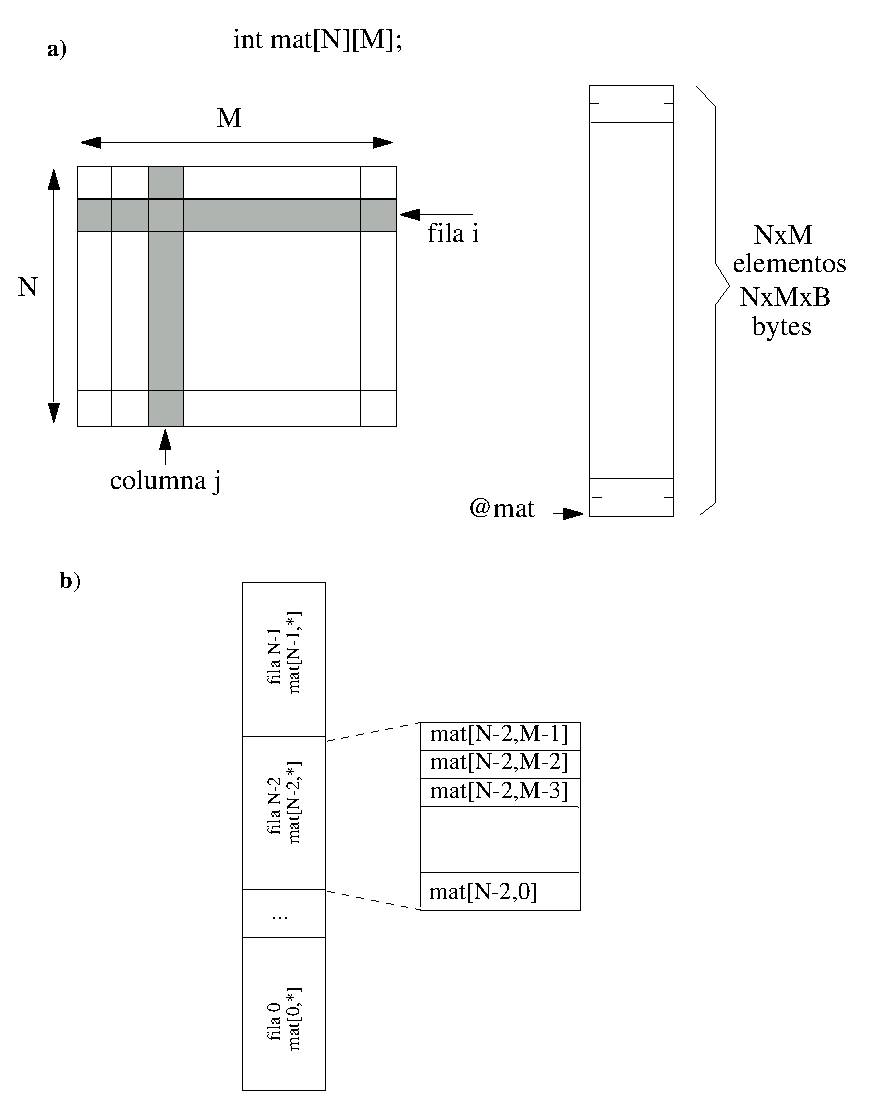
\includegraphics[width=10cm]{graphs/2-5.eps}
  \caption{(a) Formato de una matriz  C con $N$ filas y $M$ columnas y (b)
organización por filas}
  \label{fig:dos_5}
\end{figure}

Por lo tanto, para acceder al elemento {\tt mat[i][j]} hemos de saltar
$i$ filas completas (de $M$ elementos de $B$ bytes) y después $j$
elementos de $B$ bytes (suponiendo una matriz de enteros, $B= 4$ bytes). Es
decir, la fórmula para obtener el elemento {\tt mat[i][j]} será:
\begin{equation}
mat[i][j] = M_d[@mat + ((i*M)+j)*B] 
\label{eq:accesoelemmatriz}
\end{equation}


\subsection{Instrucciones de salto}

Las instrucciones de salto pueden producir saltos incondicionales ({\tt b} y {\tt bx})
o saltos condicionales. En los saltos condicionales añadimos dos o tres letras
a la ({\tt b/bx}), mediante las cuales condicionamos si se salta o no dependiendo
del estado de los flags. Estas condiciones se pueden añadir a cualquier
otra instrucción, aunque la mayoría de las veces lo que nos interesa es controlar
el flujo del programa y así ejecutar o no un grupo de instrucciones dependiendo
del resultado de una operación (reflejado en los flags).

La lista completa de condiciones es ésta.

\begin{itemize}
  \item{\tt EQ} ({\tt eq}ual, igual). Cuando {\tt Z} está activo ({\tt Z} vale 1).
  \item{\tt NEQ} ({\tt n}ot {\tt eq}ual, igual). Cuando {\tt Z} está inactivo ({\tt Z} vale 0).
  \item{\tt MI} ({\tt mi}nus, negativo). Cuando {\tt N} está activo ({\tt N} vale 1).
  \item{\tt PL} ({\tt pl}us, positivo o cero). Cuando {\tt N} está inactivo ({\tt N} vale 0).
  \item{\tt CS/HS} ({\tt c}arry {\tt s}et/{\tt h}igher or {\tt s}ame, carry activo/mayor o igual). Cuando {\tt C} está activo ({\tt C} vale 1).
  \item{\tt CC/LO} ({\tt c}arry {\tt c}lear/{\tt l}ower, carry inactivo/menor). Cuando {\tt C} está inactivo ({\tt C} vale 0).
  \item{\tt VS} (o{\tt v}erlow {\tt s}et, desbordamiento activo). Cuando {\tt V} está activo ({\tt V} vale 1).
  \item{\tt VC} (o{\tt v}erlow {\tt c}lear, desbordamiento inactivo). Cuando {\tt V} está inactivo ({\tt V} vale 0).
  \item{\tt GT} ({\tt g}reater {\tt t}han, mayor en complemento a dos). Cuando {\tt Z} está inactivo y {\tt N=V}({\tt Z} vale 0, {\tt N} vale {\tt V}).
  \item{\tt LT} ({\tt l}ower {\tt t}han, menor en complemento a dos). Cuando {\tt N!=V} ({\tt N} vale {\tt not V}).
  \item{\tt GE} ({\tt g}reater or {\tt e}qual, mayor o igual en complemento a dos). Cuando {\tt N=V}({\tt N} vale {\tt V}).
  \item{\tt LE} ({\tt l}ower or {\tt e}qual, menor o igual en complemento a dos). Cuando {\tt Z} está activo y {\tt N!=V} ({\tt Z} vale 1, {\tt N} vale {\tt not V}).
  \item{\tt HI} ({\tt h}igher, mayor). Cuando {\tt C} está activo y {\tt Z} inactivo ({\tt C} vale 1, {\tt Z} vale 0).
  \item{\tt LS} ({\tt l}ower or {\tt s}ame, menor o igual). Cuando {\tt C} está inactivo ó {\tt Z} activo ({\tt C} vale 0 ó {\tt Z} vale 1).
\end{itemize}

Por ejemplo, la instrucción {\tt beq destino\_salto} producirá un salto
a la instrucción indicada por la etiqueta {\tt destino\_salto} si y sólo
si el bit de estado cero está activo (Z=1), y en caso contrario
(Z=0) no interrumpirá el flujo secuencial de instrucciones.
Previo a un salto condicional, el registro de flags debe ser actualizado
mediante alguna instrucción aritmética ({\tt adds}, {\tt subs}, {\tt cmp},
\dots) o lógica ({\tt and}, {\tt orr}, {\tt tst}, \dots). En la mayoría
de los casos tenemos que añadir el sufijo {\tt s} a una instrucción normal
{\tt add}, para forzar que la nueva instrucción {\tt adds} actualice los flags.

El operando de la instrucción de salto ({\tt b}) puede ser una etiqueta que indica la
posición de memoria a saltar, o bien un registro en caso de {\tt bx}.

Un aspecto muy peculiar de la arquitectura ARM es que las llamadas a
subrutinas se hacen mediante un sencillo añadido a la instrucción de salto. La
instrucción {\tt bl} (también {\tt blx}) hace una llamada a una subrutina,
mediante un salto a la subrutina y escribiendo en el registro {\tt lr} la
dirección de la siguiente instrucción.

\begin{lstlisting}
main:   mov     r1, #1
        mov     r2, #2
        bl      subrut
        mov     r4, #4  /* siguiente instrucción */
        ...

subrut: mov     r3, #3
        bx      lr
\end{lstlisting}

Si seguimos el flujo del programa primero cargamos {\tt r1} a 1, luego {\tt r2}
a 2 y lo siguiente que hay es una llamada a subrutina. En dicha llamada el
procesador carga en {\tt lr} la dirección de la siguiente instrucción {\tt mov r4, \#4}
y salta a la etiqueta {\tt subrut:}. Se ejecuta el {\tt mov r3, \#3} de la subrutina
y después {\tt bx lx} que vendría a ser la instrucción de retorno. Es decir, salimos
de la subrutina retomando el flujo del programa principal, ejecutando {\tt mov r4, \#4}.

Este sencillo esquema vale para un sólo nivel de subrutinas, es decir, dentro de
{\tt subrut} no podemos llamar a otra subrutina porque sobreescribimos el valor del
registro {\tt lr}. La solución para extender a cualquier número de niveles es almacenar
el registro {\tt lr} en pila con las instrucciones {\tt push} y {\tt pop}.

\begin{lstlisting}
main:   mov     r1, #1
        mov     r2, #2
        bl      nivel1
        mov     r5, #5  /* siguiente instrucción */
        ...

nivel1: push    {lr}
        mov     r3, #3
        bl      nivel2
        pop     {lr}
        bx      lr

nivel2: mov     r4, #4
        bx      lr
\end{lstlisting}

Como véis en el último nivel ({\tt nivel2}) podemos ahorrarnos el tener que
almacenar y recuperar {\tt lr} en la pila.

\vspace{0.25cm}
Las instrucciones de salto en la arquitectura ARM abarcan una zona muy extensa,
hasta 16Mb. Sin embargo no cubren todo el ancho del bus de direcciones, sólo
24 de los 32 bits. En caso de necesitar un salto mayor de 24 bits recurrimos
a la misma solución de la carga de inmediatos del {\tt mov}, solo que el
registro a cargar es el {\tt pc}.

\begin{lstlisting}
        ldr pc, =etiqueta
\end{lstlisting}

\subsection{Estructuras de control de alto nivel}

En este punto veremos cómo se traducen a ensamblador las estructuras
de control de alto nivel que definen un bucle ({\tt for}, {\tt while},
\dots), así como las condicionales ({\tt if-else}).

Las estructuras {\tt for} y {\tt while} se pueden ejecutar un mínimo de 0
iteraciones (si la primera vez no se cumple la condición). La traducción de
las estructuras {\tt for} y {\tt while} se puede ver en los listados
\ref{lst:codigoPract2_1} y \ref{lst:codigoPract2_2}.

Para programar en ensamblador estas estructuras se utilizan instrucciones
de salto condicional. Previo a la instrucción de salto es necesario evaluar
la condición del bucle o de la sentencia {\tt if}, mediante instrucciones
aritméticas o lógicas, con el fin de actualizar los flags de estado. La
traducción de la estructura {\tt if} está en los listados
\ref{lst:codigoPract2_3} y \ref{lst:codigoPract2_4}.

\begin{lstlisting}[caption={Código del programa tipos1.c},label={lst:codigoPract2_1},escapeinside={@}{@}]
  int vi, vf, i;

  for ( i= vi; i<=vf; i++ ){ 
    /*cuerpo del bucle*/
  }

  i= vi; 
  while ( i<=vf ){ 
    /*cuerpo del bucle*/
    i++; 
  }
\end{lstlisting}

\begin{lstlisting}[caption={Traducción de las estructuras {\tt for} y {\tt while}.
Hemos supuesto que el valor inicial está en la variable {\tt vi}
y el valor final en  la variable {\tt vf} y se ha utilizado el
registro {\tt r1} como índice de las iteraciones {\tt i}.},label={lst:codigoPract2_2},escapeinside={@}{@}]
        ldr     r1, =vi
        ldr     r1, [r1]
        ldr     r2, =vf
        ldr     r2, [r2]
bucle:  cmp     r1, r2
        bhi     salir
        /* cuerpo
           del
           bucle  */
        add     r1, r1, #1
        b       bucle
salir:
\end{lstlisting}

\begin{lstlisting}[caption={Código del programa tipos2.c},label={lst:codigoPract2_3},escapeinside={@}{@}]
  int a, b;

  if( a==b ){ 
    /* código entonces */
  }
  else{
    /* código sino */
  }
\end{lstlisting}

\begin{lstlisting}[caption={Traducción de la estructura {\tt if}},label={lst:codigoPract2_4},escapeinside={@}{@}]
        ldr     r1, =a
        ldr     r1, [r1]
        ldr     r2, =b
        ldr     r2, [r2]
        cmp     r1, r2
        bne     sino
entonces:
        /* código entonces */
        b       final
sino:
        /* código sino */
final:  ...
\end{lstlisting}

\subsection{Compilación a ensamblador}

Para acabar la teoría veamos cómo trabaja un compilador de C real. Normalmente
los compiladores crean código compilado (archivos {\bf .o}) en un
único paso. En el caso de {\bf gcc} este proceso se hace en dos fases: en una
primera se pasa de C a ensamblador, y en una segunda de ensambladador a código
compilado (código máquina). Lo interesante es que podemos interrumpir justo
después de la compilación y ver con un editor el aspecto que tiene el código
ensamblador generado a partir del código fuente en C.

Veámoslo con un ejemplo.

\begin{lstlisting}[caption={Código del programa tipos3.c},label={lst:codigoPract2_5},escapeinside={@}{@}]
#include <stdio.h>

void main(void){

  int i;

  for ( i= 0; i<5; i++ ){
    printf("%d\n", i);
  }

}
\end{lstlisting}

Después de crear el fichero {\tt tipos3.s}, lo compilamos con este comando.

\begin{lstlisting}
        gcc -Os -S -o tipos3a.s tipos3.c
\end{lstlisting}

Con el parámetro {\tt -S} forzamos la interrupción (generamos {\tt .s} en lugar de
{\tt .o}) y con {\tt -Os} le indicamos al compilador que queremos optimizar en
tamaño, es decir que queremos código ensamblador lo más pequeño posible, sin
importar el rendimiento del mismo.

El código ensamblador resultante está un poco sucio, lleno de directivas superfluas,
con punteros a variables e instrucciones no simplificadas por el preprocesador. Tras
limpiarlo quedaría así.

\begin{lstlisting}[caption={Código del programa tipos3a.s},label={lst:codigoPract2_6},escapeinside={@}{@}]
.data
var1:   .asciz  "%d\012"

.text
.global main
main:   push    {r4, lr}
        mov     r4, #0
.L2:    mov     r1, r4
        ldr     r0, =var1
        add     r4, r4, #1
        bl      printf
        cmp     r4, #5
        bne     .L2
        pop     {r4, pc}
\end{lstlisting}

El carácter {\tt \textbackslash n} se ha transformado en octal {\tt \textbackslash 012} puesto que el ensamblador
no entiende de secuencias de escape. La instrucciones {\tt push} y {\tt pop} son la versión
simple de {\tt stmfd} y {\tt ldmfd} que veremos más adelante. Nótese que la función no acaba
con el típico {\tt bx lr}, se trata de una optimización que consigue reducir de dos
instrucciones a una.

\begin{lstlisting}
        pop     {r4, pc}
\end{lstlisting}

La instrucción anterior es equivalente a estas otras dos.

\begin{lstlisting}
        pop     {r4, lr}
        bx      lr
\end{lstlisting}

En general no vamos a emplear este tipo de optimizaciones en las prácticas, puesto que
dificultan la legibilidad del código.

El resto del código es sencillo de seguir. El registro {\tt r4} hace la función del
contador {\tt i} del bucle, y la salida por pantalla se produce mediante una llamada
a la función printf {\tt bl printf}. Los parámetros se los pasamos a printf mediante
{\tt r0} y {\tt r1} y son un puntero a la cadena a imprimir {\tt \%d\textbackslash n}
y el entero que le vamos a pasar. El porqué se usan estos registros para pasar
parámetros (y el hecho de
haber almacenado {\tt r4} en pila) responde a la convención {\bf AAPCS} que
veremos con más detenimiento en el siguiente capítulo.

Veamos qué ocurre cuando le indicamos al compilador que queremos optimizar al
máximo en velocidad (la escala va del 0 al 3) el mismo código en C.

\begin{lstlisting}
        gcc -O3 -S -o tipos3b.s tipos3.c
\end{lstlisting}

Tras simplificar, el fichero en ensamblador generado sería este.

\begin{lstlisting}[caption={Código del programa tipos3b.s},label={lst:codigoPract2_7},escapeinside={@}{@}]
.data
var1:   .asciz  "%d\012"

.text
.global main
main:   push    {r4, lr}
        mov     r1, #0
        ldr     r4, =var1
        mov     r0, r4
        bl      printf
        mov     r0, r4
        mov     r1, #1
        bl      printf
        mov     r0, r4
        mov     r1, #2
        bl      printf
        mov     r0, r4
        mov     r1, #3
        bl      printf
        mov     r0, r4
        mov     r1, #4
        pop     {r4, lr}
        b       printf
\end{lstlisting}

Observamos que el bucle como tal ha desaparecido. En realidad lo que ha ocurrido
es que el compilador a empleado una técnica agresiva de optimización llamada
{\it loop unrolling} o desenrollamiento de bucle, que consiste en sustituir
mediante repeticiones del cuerpo del bucle, de tal forma que no perdemos tiempo
comparando ni haciendo el salto condicional. En este caso empleamos tantas repeticiones
como iteraciones tiene el bucle, aunque normalmente se llega hasta un límite de
repeticiones. De no ser así el ejecutable se volvería excesivamente grande.

Por último señalar que se optimizado el final de la función, aunque de otra forma
distinta al caso anterior. La última iteración debería ser así.

\begin{lstlisting}
        mov     r0, r4
        mov     r1, #4
        bl      printf
        pop     {r4, lr}
        bx      lr
\end{lstlisting}

\subsection{Ejercicios propuestos.}

\subsubsection{Ejercicio 2.1}
Basándonos en los ejemplos anteriores, escribe un bucle for {\tt for} que imprima
los 50 primeros números pares naturales en orden inverso (desde 100 hasta 2 en pasos
de 2). Una vez hecho esto, aplica desenrollamiento de bucle de tal forma
que el salto condicional se ejecute 10 veces, con 5 repeticiones cada vez.

\begin{center}
\begin{myfbox}
\small
\begin{minipage}{0.92\linewidth}
\begin{center}
\colorbox[gray]{1}{\rule{0cm}{4.5cm}\rule{11cm}{0cm}}
\end{center}
\end{minipage}
\end{myfbox}
\end{center}

\subsubsection{Ejercicio 2.2}
Escribe el código ensamblador correspondiente a una estructura {\tt
if} en la que no exista la rama de {\tt else}.

\begin{center}
\begin{myfbox}
\small
\begin{minipage}{0.92\linewidth}
\begin{center}
\colorbox[gray]{1}{\rule{0cm}{4.5cm}\rule{11cm}{0cm}}
\end{center}
\end{minipage}
\end{myfbox}
\end{center}

\subsubsection{Ejercicio 2.3}

Escribe en ensamblador un código equivalente a éste. Primero
haciendo uso de la instrucción {\tt ands} y un registro auxiliar,
luego simplifica con la instrucción {\tt tst}.

\begin{center}
\begin{myfbox}
\small
\begin{minipage}{0.92\linewidth}
\begin{center}
\begin{minipage}{0.6\linewidth}
\begin{verbatim}
  for ( i= 0; i<10; i++ ){
    if( i&1 )
      printf("%d es impar\n", i);
    else
      printf("%d es par\n", i);
  }
\end{verbatim}
\end{minipage}
\end{center}
\begin{center}
\colorbox[gray]{1}{\rule{0cm}{7cm}\rule{11cm}{0cm}}
\end{center}
\end{minipage}
\end{myfbox}
\end{center}

\subsubsection{Ejercicio 2.4}

Escribe en ensamblador la estructura de alto nivel {\tt switch},
aplicándola al siguiente ejemplo en C.

\begin{center}
\begin{myfbox}
\small
\begin{minipage}{0.92\linewidth}
%\begin{center}
\begin{minipage}{0.6\linewidth}
\begin{verbatim}
  for ( i= 1950; i<2015; i++ ){
    switch( i&3 ){
      case 0:  printf("En %d hubo olimpiadas\n", i);
               break;
      case 2:  printf("En %d hubo mundial de fútbol\n", i);
               break;
      default: printf("En %d no pasó nada\n", i);
    }
  }
\end{verbatim}
\end{minipage}
%\end{center}
\begin{center}
\colorbox[gray]{1}{\rule{0cm}{7cm}\rule{11cm}{0cm}}
\end{center}
\end{minipage}
\end{myfbox}
\end{center}

\section{Enunciados de la práctica}


\subsection{Suma de elementos de un vector}

En este primer apartado, estudiaremos un bucle que calcula la suma de
todos los elementos de un vector. El vector se denomina {\tt
vector} y tiene 5 elementos de tipo {\tt int} (entero de 32 bits). Los algoritmos
que realizan la suma de sus elementos, tanto en C como en ensamblador, se
pueden encontrar en los listados \ref{lst:dos_9} y \ref{lst:dos_10}.

\begin{lstlisting}[caption={Código del programa tipos4.c},label={lst:dos_9},escapeinside={@}{@}]
#include <stdio.h>

void main(void){
  int i, suma;
  int vector[5]= {128, 32, 100, -30, 124};

  for ( suma= i= 0; i<5; i++ ){
    suma+= vector[i];
  }
  printf("La suma es %d\n", suma);
}
\end{lstlisting}

\begin{lstlisting}[caption={Código del programa tipos4.s},label={lst:dos_10},escapeinside={@}{@}]
.data
var1:   .asciz  "La suma es %d\n"
var2:   .word   128, 32, 100, -30, 124

.text
.global main
main:   push    {r4, lr}
        mov     r0, #5
        mov     r1, #0
        ldr     r2, =var2
bucle:  ldr     r3, [r2], #4
        add     r1, r1, r3
        subs    r0, r0, #1
        bne     bucle
        ldr     r0, =var1
        bl      printf
        pop     {r4, lr}
        bx      lr
\end{lstlisting}

Si analizamos el código en ensamblador (listado \ref{lst:dos_10}(b)), veremos que se
recorre todo el vector con el registro {\tt r0}, realizándose la suma sobre el
registro {\tt r1}. A diferencia de ejemplos anteriores decrementamos de 5 a 0, así
nos ahorramos una comparación, ya que la instrucción {\tt subs} detecta cuando hemos
llegado al valor cero activando el flag {\tt Z}.

En {\tt r2} vamos recorriendo el vector elemento a elemento mediante un modo postindexado
que apunta al siguiente elemento una vez leemos el actual con {\tt ldr}. Una vez calculada
la suma en {\tt r1}, la mostramos por pantalla mediante una llamada a {\tt printf}.

El código del listado \ref{lst:dos_10} está en el fichero {\tt tipos4.s}. Compila y
monta el programa con el {\tt as} y el {\tt gcc}. Ahora ejecuta el algoritmo
con el {\tt gdb}. Recuerda empezar con {\tt start}. Para ver su funcionamiento,
podemos ejecutar un par de iteraciones con {\tt si} y ver cómo los valores de
los registros van cambiando {\tt i r r0 r1 r2 r3} (de vez en cuando ejecuta
{\tt disas} para saber por dónde vas). Si ejecutamos un par de iteraciones con
{\tt si} veremos que el hecho de ejecutar instrucción a instrucción resulta
poco útil. Para acelerar el proceso, podemos utilizar puntos de parada o {\it breakpoints}.

Otro problema que tenemos es que al ejecutar un paso de una instrucción exacta {\tt si}
nos metemos dentro de la rutina {\tt printf}, cosa que no nos interesa a no ser que queramos
descubrir las interioridades de la librería. Para evitar esto ejecutamos con {\tt ni}, que
ejecutará {\tt bl printf} de un paso sin meterse dentro.

Para introducir un breakpoint hay varias maneras, siempre es buena idea investigar a fondo
la ayuda que se nos brinda el propio depurador con {\tt help break}. Nosotros pondremos dos
puntos de ruptura.

\begin{lstlisting}
(gdb) start
Temporary breakpoint 1 at 0x83cc
Starting program: /home/pi/tipos4

Temporary breakpoint 1, 0x000083cc in main ()
(gdb) break bucle
Breakpoint 2 at 0x83dc
(gdb) disas bucle
Dump of assembler code for function bucle:
   0x000083dc <+0>:     ldr     r3, [r2], #4
   0x000083e0 <+4>:     add     r1, r1, r3
   0x000083e4 <+8>:     subs    r0, r0, #1
   0x000083e8 <+12>:    bne     0x83dc <bucle>
   0x000083ec <+16>:    ldr     r0, [pc, #12]
   0x000083f0 <+20>:    bl      0x82f0 <printf>
   0x000083f4 <+24>:    pop     {r4, lr}
   0x000083f8 <+28>:    bx      lr
   0x000083fc <+32>:                    ; <UNDEFI..
   0x00008400 <+36>:    andeq   r0, r1, r4, lsr #11
End of assembler dump.
(gdb) break *0x83ec
Breakpoint 3 at 0x83ec
\end{lstlisting}

Ahora toca continuar la ejecución del programa hasta el final o hasta llegar a
un punto de ruptura, y esto se hace con {\tt continue} (de forma abreviada {\tt cont}).
También podemos mostrar la lista de puntos de ruptura, desactivar temporalmente un breakpoint
o simplemente borrarlo.

\begin{lstlisting}
(gdb) info breakpoints
Num     Type           Disp Enb Address    What
2       breakpoint     keep y   0x000083dc <bucle>
3       breakpoint     keep y   0x000083ec <bucle+16>
(gdb) disable 2
(gdb) delete 3
(gdb) i b
Num     Type           Disp Enb Address    What
2       breakpoint     keep n   0x000083dc <bucle>
\end{lstlisting}

Antes de acabar nuestra sesión con {\tt gdb} depuramos la última iteración del bucle,
y luego dos instrucciones más para mostrar el texto que emite {\tt printf}.

\begin{lstlisting}
(gdb) i r r0 r1
r0             0x1      1
r1             0xe6     230
(gdb) disas
Dump of assembler code for function bucle:
=> 0x000083dc <+0>:     ldr     r3, [r2], #4
   0x000083e0 <+4>:     add     r1, r1, r3
   0x000083e4 <+8>:     subs    r0, r0, #1
   0x000083e8 <+12>:    bne     0x83dc <bucle>
   0x000083ec <+16>:    ldr     r0, [pc, #12]
   0x000083f0 <+20>:    bl      0x82f0 <printf>
   0x000083f4 <+24>:    pop     {r4, lr}
   0x000083f8 <+28>:    bx      lr
End of assembler dump.
(gdb) ni 4
0x000083ec in bucle ()
(gdb) i r r1 r3
r1             0x162    354
r3             0x7c     124
(gdb) ni 2
La suma es 354
0x000083f4 in bucle ()
\end{lstlisting}

Ahora vamos a modificar un poco el programa. Copiamos {\tt tipos4.s} en
otro fichero {\tt tipos4.s} (con {\tt cp tipos4.s tipos5.s}). Ahora modifica
la lista de números del array, reemplazándola por esta otra.

\begin{lstlisting}
var2:   .word   1600000000, -100, 800000000, -50, 200
\end{lstlisting}

Haz el ejercicio 2.5 y acábalo antes de seguir.\vspace{0.25cm}

\subsubsection{Ejercicio 2.5}
Sabiendo que la suma de los 5 elementos del vector anterior es
2.400.000.050 completa el siguiente cuadro:

\colorbox[gray]{0.9}{
\small
%\arrayrulecolor{black}
\begin{tabular}{c}
\begin{minipage}{0.9\linewidth}
Traduce el número 2.400.000.050 a binario: \\\\
\colorbox[gray]{1}{\rule{0cm}{0.46cm}\rule{11.25cm}{0cm}}\\
\end{minipage} \\
\begin{minipage}{0.9\linewidth}
Interpreta el resultado como un entero de 32 bits y tradúcelo a
decimal, ¿cuánto da? \\\\
\colorbox[gray]{1}{\rule{0cm}{0.46cm}\rule{11.25cm}{0cm}}\\\\
¿Se puede representar el número entero 2.400.000.050 con 32 bits? \\\\
\colorbox[gray]{1}{\rule{0cm}{0.46cm}\rule{11.25cm}{0cm}}\\
\end{minipage} \\
\end{tabular}
\vspace{0.5ex}
}

\vspace{0.25cm}
Si has hecho el ejercicio 2.5 puedes ahora comprobar que la suma de
los valores de este vector produce un {\it overflow} sobre un {\tt
int}. Por tanto, el programador debería ir acumulando el resultado de
la suma sobre un {\tt long long} (64 bits), tal y como se muestra
en el siguiente listado.

\begin{lstlisting}
void main(void){
  int i;
  long long suma;
  int vector[5]= {1600000000, -100, 800000000, -50, 200};

  for ( suma= i= 0; i<5; i++ ){
    suma+= vector[i];
  }
  printf("La suma es %d\n", suma);
}
----------------
.data
var1:   .asciz  "La suma es %lld\n"
var2:   .word   1600000000, -100, 800000000, -50, 200

.text
.global main
main:   push    {r4, r5, r6, lr}
        mov     r5, #5
        mov     r2, #0
        mov     r3, #0
        ldr     r4, =var2
bucle:  ldr     r0, [r4], #4
        mov     r1, r0, ASR #31
        adds    r2, r2, r0
        adc     r3, r3, r1
        subs    r5, r5, #1
        bne     bucle
        ldr     r0, =var1
        bl      printf
        pop     {r4, r5, r6, lr}
        bx      lr
\end{lstlisting}

En el código ensamblador la variable suma se almacena en los registros {\tt r3:r2}.
Como el array almacenado en memoria es de 32 bits, lo que hacemos es cargar el valor
en cada iteración en {\tt r0} y extender el signo mediante la instrucción
{\tt mov r1, r0, ASR \#31} a los registros {\tt r1:r0}. Por último hacemos la suma
{\tt r3:r2= r3:r2+r1:r0} mediante dos instrucciones de suma, en la primera {\tt adds}
sumamos los 32 bits inferiores almacenando también el posible acarreo (flag {\tt C}),
y en la segunda {\tt adc} sumamos los 32 bits superiores más el acarreo anterior.

Sin entrar en detalles que veremos en el próximo capítulo, el número de 64 bits que
le enviamos a la función {\tt printf} debe estar {\tt r3:r2}, debemos guardar en pila
todos los registros por encima de {\tt r4} (incluyéndolo) y en el {\tt push} debe
haber un número par de elementos. Si tuviésemos un número impar, como es el caso,
salvaremos el siguiente registro {\tt r6} aunque no lo necesitemos en nuestra función.



\subsubsection{Ejercicio 2.6}
Dada la definición de matriz {\tt short mat[4][6]}; ¿cuál es la
fórmula para acceder al elemento {\tt mat[i][2]}?

\begin{center}
\colorbox[gray]{0.9}{
%\arrayrulecolor{black}
\small
\begin{tabular}{c}
%\rowcolor{white} 
\\
\begin{minipage}{0.9\linewidth}
\colorbox[gray]{1}{\rule{0cm}{0.6cm}\rule{11cm}{0cm}}\\
\end{minipage} \\
\end{tabular}
\vspace{0.5ex}
}
\end{center}


\begin{lstlisting}[caption={Matrices},label={lst:dos_11},escapeinside={@}{@}]
matriz: .hword    0,    1,    2,    3,    4,    5
        .hword 0x10, 0x11, 0x12, 0x13, 0x14, 0x15
        .hword 0x20, 0x21, 0x22, 0x23, 0x24, 0x25
        .hword 0x30, 0x31, 0x32, 0x33, 0x34, 0x35
suma:   .hword 0
------------------------------
suma= 0; 
for ( i= 0; i<4; i++ ){
  suma+= mat[i][2];
}
\end{lstlisting}

Queremos hacer un programa que sume todos los elementos de la columna
2 de la matriz (listado \ref{lst:dos_11}). Completa {\tt tipos7.s} para
que implemente este código, utilizando dentro del bucle que realiza la
suma la fórmula del ejercicio 2.6. Para comprobarlo, el resultado
es 104 = 0x68.

Fíjate en que en esta versión del código que recorre los elementos de
una columna,  para calcular la dirección de cada elemento aplicamos la
expresión \ref{eq:accesoelemmatriz}. A ésto es a lo que llamamos
acceso aleatorio a los elementos de la matriz. 

Sin embargo, sabemos que hay una relación entre los elementos de una
fila y de la siguiente, cuando el tamaño de la columna es
constante. Para hallar esta relación haz siguiente ejercicio.

\subsubsection{Ejercicio 2.7}

Calcula las fórmulas de acceso a  {\tt mat[i][2]} y  {\tt mat[i+1][2]} y
halla su diferencia (resta las dos fórmulas).

\vspace{0.25cm}
\colorbox[gray]{0.9}{
\small
%\arrayrulecolor{black}
\begin{tabular}{c}
\\
%\rowcolor{white} 
\begin{minipage}{0.9\linewidth}
\colorbox[gray]{1}{\rule{0cm}{0.6cm}\rule{11cm}{0cm}}\\
\end{minipage} \\
\end{tabular}
\vspace{0.5ex}
}

\vspace{0.25cm} 

Una vez hallada esta relación, que es un desplazamiento en memoria,
ahora sabes que se pueden recorrer todos los elementos de una columna
sin más que ir sumando ese desplazamiento. Decimos entonces que
hacemos un acceso secuencial a los elementos de la matriz. Copia el
fichero {\tt tipos7.s} a {\tt tipos8.s} e implementa sobre este
último  el acceso secuencial. El resultado es el anterior (104 = 0x68).

\chapterend{}

%%%%%%%%%%%%%%%%%%%%%%%%%%%%%%%%%%%%%%%%%%%%%%%%%%%%%%%%%%%%%%
\end{document}

% Capítulo 03.
\documentclass[12pt,a4paper]{book} % article, report, book.
%%%%%%%%%%%%%%%%%%%%%%%%%%%%%%%%%%%%%%%%%%%%%%%%%%%%%%%%%%%%%%%%%%%
%%% Documento LaTeX                                             %%%
%%%%%%%%%%%%%%%%%%%%%%%%%%%%%%%%%%%%%%%%%%%%%%%%%%%%%%%%%%%%%%%%%%%
% Título: Paquetes
% Autor:  Ignacio Moreno Doblas
% Fecha:  2014-02-01
%%%%%%%%%%%%%%%%%%%%%%%%%%%%%%%%%%%%%%%%%%%%%%%%%%%%%%%%%%%%%%%%%%%
% Tabla de materias:
% 1 Codificación e idioma %
% 2 Matemáticas y Física %
% 3 Gráficos%
% 4 Estilo y formato%
%%%%%%%%%%%%%%%%%%%%%%%%%%%%%%%%%%%%%%%%%%%%%%%%%%%%%%%%%%%%%%%%%%%

%1 Codificación e idioma%
\usepackage[utf8]{inputenc} %Codificación en utf8%
\usepackage[spanish]{babel} %Hyphenation (Guionado) en español%
\usepackage[T1]{fontenc} %Codificación de fuente%
\usepackage{eurofont} %Tipografía euro (€)%

%2 Matemáticas y Física %
% Importante para ecuaciones, magnitudes y unidades%
\usepackage{amssymb,amsmath,latexsym,amsfonts} % paquetes estándar%
\usepackage[squaren]{SIunits} %Paquete para magnitudes y unidades físicas%
\usepackage{ifthen} %sentencias if y while%

%3 Gráficos%
\usepackage{graphics,graphicx} %paquetes gráficos estándar%
\usepackage{wrapfig} %paquete para gráfica lateral%
\usepackage[rflt]{floatflt} %figuras flotantes%
  % \begin{floatingfigure}[r]/[l]{4.5cm}
  % \end{floatingfigure}
\usepackage{graphpap} %comando \graphpaper en el entorno picture%

%4 Estilo y formato%
\usepackage{fancyhdr} %cabeceras y pies mejor que con \pagestyle{}%
\usepackage{titlesec,titletoc} %Formateo de secciones y títulos%
\raggedbottom %Para fragmentar versos en varias páginas%
\usepackage{makeidx} %MakeIndex%
%\usepackage{showidx} % Hace que cada comando \index se imprima en la página donde se ha puesto (útil para corregir los índices)
\usepackage{alltt} % Define el environment alltt, como verbatim, excepto que \, { y } tienen su significado normal. Se describe en el fichero alltt.dtx.
\usepackage[pdftex,bookmarksnumbered,hidelinks]{hyperref} %hyper-references%
\usepackage{minitoc} % Para poner tablas de contenido en cada capítulo.
\usepackage{listings} % Para escribir piezas de código C, Python, etc. %
%listings configuration
\lstset{
  language=[ARM]Assembler, %Puede ser C, C++, Java, etc.
  showstringspaces=false,
  formfeed=\newpage,
  tabsize=4,
  commentstyle=\itshape,
  basicstyle=\ttfamily,
  morekeywords={models, lambda, forms}
}

\usepackage{tipa} % tipografía IPA (International Phonetic Alphabet)
\usepackage{longtable} %Entorno Longtable, fracciona tablas a lo largo de páginas%
\usepackage{colortbl}
\usepackage{acronym}  %Para expandir automáticamente los acrónimos

%%%%%%%%%%%%%%%%%%%%%%%%%%%%%%%%%%%%%%%%%%%%%%%%%%%%%%%%%%%%%%%%%%%
% Tabla de materias:
% 1 Información del Documento %
% 2 Comandos a nivel de texto %
% 3 Comandos a nivel de entorno %
% 4 Comandos a nivel de página y sección %
% 5 Otros comandos %
%%%%%%%%%%%%%%%%%%%%%%%%%%%%%%%%%%%%%%%%%%%%%%%%%%%%%%%%%%%%%%%%%%%

% 1 Información del Documento %
\newcommand{\pfctitlename}{Guiones de prácticas sobre la plataforma Raspberry Pi}
\newcommand{\pfcauthorname}{Antonio José Villena Godoy}
\newcommand{\pfctutorname}{Rafael Asenjo Plaza \\ Francisco Javier Corbera Peña}
\newcommand{\pfcanno}{2015}

% 2 Comandos a nivel de texto %
\newcommand{\R}{\textsuperscript{\textregistered}}  %Símbolo registrado%
\newcommand{\C}{\textsuperscript{\copyright}} %Símbolo Copyright%
\newcommand{\TM}{\texttrademark} %Símbolo Trade Mark (marca comercial)%

% 2.1 Comandos abreviatura %
\newcommand{\tit}{\textit} %Fuente cursiva (itálica)%
\newcommand{\tbf}{\textbf} %Fuente negrita%
\newcommand{\ttw}[1]{\texttt{#1}} %Fuente máquina de escribir (typewriter)%
%Combinación%
\newcommand{\textittt}[1]{\textit{\texttt{#1}}} %itálica y typewriter%
\newcommand{\textittw}{\textittt} % Otra forma de escribirlo.
\newcommand{\tittw}{\textittw} %Shortened%
\newcommand{\tbftw}[1]{\tbf{\ttw{#1}}}

%Crea una nueva línea y la indenta sin crear interlineado extra.
\newcommand{\nli}{\\ \indent} 

%Para escribir un correo electrónico%
\newcommand{\mailto}[1]{\href{mailto:#1}{#1}}

% Si vas a hacer un uso básico de \index (entradas en el índice de sólo un nivel, sin formatos especiales, etc.), define la orden
\newcommand{\miindex}[1]{#1\index{#1}}

\newcommand{\hs}{\hspace} % Abreviatura espacio horizontal
\newcommand{\vs}{\vspace} % Abreviatura espacio vertical

% Abreviaturas para los conjuntos de números más comunes.
\newcommand{\realnumbers}{\mathbb R}
\newcommand{\naturalnumbers}{\mathbb N}
\newcommand{\integernumbers}{\mathbb Z}
\newcommand{\rationalnumbers}{\mathbb Q}
\newcommand{\complexnumbers}{\mathbb R}
\newcommand{\irrationalnumbers}{\mathbb I}

% Doble barra sobre una letra (para expresar las matrices).
\newcommand{\doublebar}[1]{\bar{\bar{#1}}} 
% Ej: \vector(y) = \doublebar(A) \vector(x) (Stma. lineal de ec.)

% 3 Comandos a nivel de entorno %
\newcommand{\benu}{\begin{enu}} % Begin enumerate
\newcommand{\eenu}{\end{enu}}   % End enumeration

%Comando para escribir código Python
\newcommand{\code}[3]{
  %\hrulefill
  %\subsection*{#1}
  %\subsubsection{#1}
  \lstinputlisting{#2}
  %#1\\
  \begin{table}[h!]
    \centering
    \caption{#1}
    \label{#3}
  \end{table}
  \vspace{2em}
}

% 4 Comandos a nivel de página y sección %
%Crea página en blanco
\newcommand{\blankpage}{\clearpage{\pagestyle{empty}\cleardoublepage}}

% Versión x del comando section: sin numeración pero sí aparece en la tabla de contenidos.
\newcommand{\sectionx}[1]{
  \section*{#1}
  \addcontentsline{toc}{section}{#1}
}

% Versión y del comando section: sin numeración y NO aparece en la tabla de contenidos.
\newcommand{\sectiony}[1]{
  \section*{#1}
}

% Versión x del comando chapter: sin numeración pero sí  aparece en la tabla de contenidos.
\newcommand{\chapterx}[1]{
  \chapter*{#1}
  %\addcontentsline{toc}{chapter}{#1} %Caused by minitoc package%
  \addstarredchapter{#1} %For minitoc package%
}

% substituto del comando \chapter: incluye estilo de página.
\newcommand{\chapterbegin}[1]%
  {%
    \pagestyle{fancy}
    \fancyhead[LE,RO]{\thepage}
    \fancyhead[LO]{Capítulo \thechapter. #1}
    %\fancyhead[RE]{Parte \thepart \rightmark} %
    \fancyhead[RE]{\nouppercase{\rightmark}} %
        
    \chapter{#1}
  }

% Versión x del comando \chapterbegin: sin numeración y aparece en la tabla de contenidos.
\newcommand{\chapterbeginx}[1]%
  {%
    \pagestyle{fancy}
    \fancyhead[RO,LE]{\thepage}
    \fancyhead[RE,LO]{#1}
    %\fancyhead[LO]{Chapter \thechapter}
    %\fancyhead[RE]{Part \thepart} %
    
    \chapterx{#1}
  }

%Fin de capítulo
\newcommand{\chapterend}{\pagestyle{empty}\cleardoublepage \thispagestyle{empty}}
%Si fuera un artículo en lugar un libro, \clearpage en lugar de \cleardoublepage

% 5 Otros comandos %
%\let\Oldpart\part
%\newcommand{\parttitle}{}
%\renewcommand{part}[1]{\Oldpart{#1}\renewcommand{\parttitle}{#1}} %Header customization%

%Cambiar el título índice de capítulo a ``Contenido''.
\renewcommand{\mtctitle}{Contenido}

\dominitoc % Para tablas de contenidos por capítulo.

\addto{\captionsspanish}{
  \renewcommand{\listtablename}{Índice de Tablas}
  \renewcommand{\tablename}{Tabla} } % Por ejemplo, modificar el nombre de 'Cuadro' a 'Tabla'.

\addto{\captionsspanish}{
  \renewcommand{\contentsname}{Índice} }

%Si se desea cambiar el tipo de letra a Arial
% por cualquier razón, descomentar las siguientes
% dos líneas
%\renewcommand{\rmdefault}{phv} % Arial
%\renewcommand{\sfdefault}{phv} % Arial
  
%\addto{\captionsspanish}{
% \renewcommand{\partname}{Fase} }

%\addto{\captionsspanish}{%
%    \renewcommand{\refname}{\vspace{-4.5ex}}} % Para que no aparezca el texto 'referencias' en la bibliografía.

% Modifica el interlineado
%\renewcommand{\baselinestretch}{1.5}

   \definecolor{myfboxbg}{gray}{0.9}
   \newsavebox{\efcaja}
   \newenvironment{myfbox}{\begin{lrbox}{\efcaja}}
               {\end{lrbox}{\colorbox{myfboxbg}{\usebox{\efcaja}}}}

%%%%%%%%%%%%%%%%%%%%%%%%%%%%%%%%%%%%%%%%%%%%%%%%%%%%%%%%%%%%%%%%%%%
% Tabla de materias:
%--------------------%
% 1 dobleindent
% 2 izqindent
% 3 dobleindentx
% 4 ite
% 5 descript
% 6 enu
% 7 itemization
% 8 sinopsis
% 9 objetivo
%%%%%%%%%%%%%%%%%%%%%%%
% Para conocer los parámetros de diseño de las listas, tales como
%  los márgenes izquierdo, derechos y los diferentes saltos,
%  véase el archivo ``List layout.png'' que acompaña esta plantilla.
% Así se conocerá mejor cómo adaptar un entorno según los requisitos 
%  del usuario.

%%%%%%%%%%%%%%%%%%%%%%%
% Definición de longitudes para usar en los entornos:
%
% Normal parskip.
\newlength{\parskipenv}
\setlength{\parskipenv}{\parskip}

\newlength{\parindentenv}
\setlength{\parindentenv}{\parindent}
%%%%%%%%%%%%%%%%%%%%%%%

% 1 dobleindent
%El entorno dobleindent está pensando para escribir párrafos con doble indentación a cada lado.
%Tiene dos parámetros de entrada con las distancias medidas desde los márgenes de página.

\newenvironment{dobleindent}[2]
  %Comienzo de nuevo entorno%
  {
  \begin{list}
    {}
    {
    % Left and right margins:
    \leftmargin = #1 
    \rightmargin = #2
    %
    % Separation from preceding and following text:
    \topsep = 0ex
    \partopsep = 0ex
    \parsep = \parskipenv
    %
    % Indentation for paragraphs:
    \itemsep = \parskipenv
    \itemindent = \parindentenv
    \listparindent = \itemindent
    %
    % Horizontal separation from label:
    \labelsep = 1ex
    \settowidth{\labelwidth}{0cm}
    }
    
     \item}
  % End new env
  {\end{list}}

%%%%%%%%%%%%%%%%%%%%%%%%%%%%%
%2 izqindent
% El entorno izqindent sólo crea un párrafo indentado a la izquierda.
\newenvironment{izqindent}[1]
{
\begin{dobleindent}{#1}{0cm}
}
{
\end{dobleindent}
}

%%%%%%%%%%%%%%%%%%%%%%%%%%%%%
% 3 dobleindentx
% El entorno dobleindentx es una variación del dobleindent usando leftskip y rightskip.
% Aunque es más limitado, también se puede usar.
\newenvironment{dobleindentx}[2] % Sólo funciona en modo paragraph
{ % Preamble
  \leftskip = #1
  \rightskip = #2
}
{ % Postamble
\leftskip = 0cm
\rightskip = 0cm
}

%%%%%%%%%%%%%%%%%%%%%%%%%%%%%
% 4 ite
% El entorno ite es una modificación del entorno itemize estándar de \LaTeX. Puede usarse o modificarse si el usuario lo desea.
% También puede parametrizarse el entorno enumerate o description de forma equivalente.
\newenvironment{ite}
  {
    \begin{izqindent}{\parindent}
    \hspace{-\parindent}  % compensación del sangrado que introduce el entorno.
    \vspace{-1.0\parskip} % compensación del \parskip que introduce el entorno.
    \vspace{-\baselineskip} % compensación por la línea que introduce el entorno.
    \begin{itemize}
  }
  {
    \end{itemize}
    \end{izqindent}
  }

%%%%%%%%%%%%%%%%%%%%%5
% commando stdformat para formatear los entornos descript, enu y itemization.
\newcommand{\stdformat}
  {% Declarations for format presentation.
    %     
    % Separation from preceding and following text:
    \setlength{\topsep}{0ex}%
    \setlength{\partopsep}{0ex} %
    %
    % Horizontal separation from label:
    \labelsep = 1ex
    \setlength{\labelwidth}{0ex}
    %
    % Left and right margins: 
    \setlength{\leftmargin}{1cm}%
    \addtolength{\leftmargin}{\labelsep}
    \setlength{\rightmargin}{0ex}
    %  
    % Indentation for paragraphs:
    \setlength{\itemindent}{-\leftmargin}%
    \addtolength{\itemindent}{1ex}
    \setlength{\listparindent}{\parindent}%
    %   
    % Separation between paragraphs.
    \setlength{\parsep}{\parskipenv}% 
    \setlength{\itemsep}{1ex}
  }

%%%%%%%%%%%%%%%%%%%%%%%%%%%%%
% 5 descript

\newenvironment{descript}
  % Beginning new env def.
  {
    \begin{list}
      {} % No default label for \item.
      {
        % Declarations for format presentation.
        \stdformat
        %
        \renewcommand{\makelabel}[1]{\normalfont\bfseries##1\hfil}
      }
  }
  % Ending new env def.
  {
    \hspace*{\fill} \\ \end{list}
  } % Se introduce un salto de línea para que el texto siguiente esté separado.
%END newenvironment{descript}

%%%%%%%%%%%%%%%%%%%%%%%%%%%%%
% 6 enu
\newcounter{itemnumber} % Counter for the environment.

\newenvironment{enu}
  % Beginning new env def.
  {
    \begin{list}
    {
      \raggedleft \arabic{itemnumber}
    }
    {
      \usecounter{itemnumber}
      \stdformat
    }
  }
  {
    \end{list}
  }

%%%%%%%%%%%%%%%%%%%%%%%%%%%%%
% 7 itemization
\newenvironment{itemization}
  % Beginning new env def.
  {
    \begin{list}
      {$\bullet$} % No default label for \item.
      {
        % Declarations for format presentation.
        \stdformat
      }
  }
  % Ending new env def.
  {
    \end{list}
  }


%%%%%%%%%%%%%%%%%%%%%%%%%%%%%
% 8 sinopsis
\newenvironment{sinopsis}{%[1]{
  \sectiony{Sinopsis}
  %\label{#1}
} {
  \pagebreak
}

%%%%%%%%%%%%%%%%%%%%%%%%%%%%%
% 9 objetivo
\newenvironment{objetivo}{%[1]{
  \sectiony{Objetivo}
  %\label{#1}
} {
}

%%%%%%%%%%%%%%%%%%%%%%%%%%%%%%%%%%%%%%%%%%%%%%%%%%%%%%%%%%%%%%%%%%%
% Tabla de materias:
%--------------------%
% 1 Márgenes de página
%%%%%%%%%%%%%%%%%%%%%%%
% Para conocer los parámetros de diseño de páginas, tales como
%  los márgenes izquierdo, derecho, anchura de página, etc.
%  véase el archivo ``Page layout.png'' que acompaña esta plantilla.
% Así se conocerá mejor cómo adaptar el documento según los 
%  requisitos del usuario.

% 1 Márgenes de página
%-------------------------------%
% Parámetros de estilo de página.
% DIN A4: 29.7 cm x 21 cm
%   área neta: 3 cm + 3 cm + 15 cm.
%
% Definición de márgenes de página
%  even para páginas pares
%  odd  para páginas impares
\newlength{\realoddsidemargin}    % \oddsidemargin menos 1 in.
\newlength{\realevensidemargin}   % \evensidemargin menos 1 in.
\newlength{\realtopmargin}        % \topmargin menos 1 in.
%
% Asignación de márgenes de página
% ASIGNESE en caso de querer cambiarlo
\setlength{\realtopmargin}{2cm}     % REAL top margin.
\setlength{\realoddsidemargin}{3cm}   % REAL oddside margin.
\setlength{\realevensidemargin}{3cm}  % REAL evenside margin.
\setlength{\hoffset}{0cm}
\setlength{\voffset}{0cm}
%
% Substracción de 1 pulgada de compensación
%  (véase ``Page Layout.png'' para más información)
\addtolength{\realoddsidemargin}{-1in}  % 1 inch = 2.54 cm.
\addtolength{\realevensidemargin}{-1in}
\addtolength{\realtopmargin}{-1in}
%
% Asignación de anchuras y márgenes
% No hay notas al margen
\setlength{\marginparsep}{0cm} % No van a existir notas al margen
\setlength{\marginparwidth}{0cm} % No van a existir notas al margen
%
% Asignación de anchura de texto
\setlength{\textwidth}{15cm}  % Anchura neta del texto (globalmente).
%
% Asignación de márgenes par, impar y en altura
\setlength{\oddsidemargin}{\realoddsidemargin}  % odd-page left margin (global).
\setlength{\evensidemargin}{\realoddsidemargin} % even-page left margin (global).
\setlength{\topmargin}{\realtopmargin}          % top margin (Global).

% Se puede usar también el paquete chngpage.

%%%%%%%%%%%%%%%%%%%%%%%%%%%%%%%%%%%%%%%%%%%%%%%%%%%%%%%%%%%%%%%%%%
%   1 Length commands.          %
%-------------------------------%
% Defines new length command (e.g., \newlength{\gnat}}
% \newlength{}
%
% Set lenght to a value.
% \setlength{\gnat}{length}
% \addtolength{}{}
%
% Sets the value of a length command equal to the width of a specified piece of text; e.g., \settowidth{\parindent}{\em small}.
% \settowidth{}{}
% Set the value of a height. e.g., \settoheight{\parskip}{Gnu}
% \settoheight{}{}
% Set the value that extends below the line. e.g., \settodepth{\parskip}{gnu}.
% \settodepth{}{}
%
% To multiply a length, write: 7.0\gnat = \gnat * 7.0
%%%%%%%%%%%%%%%%%%%%%%%%%%%%%%%%%%%%%%%%%%%%%%%%%%%%%%%%%%%%%%%%%%

\begin{document}

\chapterbegin{Subrutinas y paso de parámetros}
\label{chp:Subrut}
\minitoc

{\bf Objetivos}: En esta sesión experimentaremos con las
subrutinas. Veremos en qué consiste la convención AAPCS y cómo
aplicarla tanto para llamar a funciones externas como para crear
nuestras propias funciones. Escribiremos un programa en C que llame
a funciones escritas en ensamblador. Por último explicaremos qué
son los registros de activación y cómo aplicarlos para almacenar
variables locales.

\section{Lectura previa}

\subsection{La pila y las instrucciones {\tt ldm} y {\tt stm}}

Se denomina pila de programa a aquella zona de memoria, organizada de
forma LIFO ({\it Last In, First Out}), que el programa emplea
principalmente para el almacenamiento temporal de datos.
%
Esta pila, definida en memoria, es fundamental para el funcionamiento
de las rutinas%
\footnote{
En este texto usaremos el término rutina (o subrutina) 
como la implementación
a bajo nivel de lo que en alto nivel se conoce como procedimientos
y funciones. La diferencia entre procedimiento y función, radica
en que las funciones proporcionan un valor de retorno. 
}%
, aspecto que se desarrollarán en esta
práctica.

El puntero de pila es {\tt r13} aunque por convención nunca se emplea esa
nomeclatura, sino que lo llamamos {\tt sp} ({\bf s}tack {\bf p}ointer o puntero
de pila). Dicho registro apunta siempre a la palabra de memoria que corresponde
a la cima de la pila (última palabra introducida en ella).

La pila tiene asociadas dos operaciones: {\tt push} (meter un elemento en la pila) y
{\tt pop} (sacar un elemento de la pila). En la operación {\tt push} primero
decrementamos en 4 (una palabra son 4 bytes) el registro {\tt sp} y luego escribimos
dicho elemento en memoria. Decimos que la pila crece hacia abajo.

\begin{lstlisting}[caption={Operación push},escapeinside={@}{@}]
        sub     sp, sp, #4
        str     r0, [sp]
\end{lstlisting}

Para sacar elementos de la pila tenemos la operación {\tt pop}, que primero extrae
el elemento de la pila y luego incrementa el puntero (decrece hacia arriba).

\begin{lstlisting}[caption={Operación pop},escapeinside={@}{@}]
        ldr     r0, [sp]
        add     sp, sp, #4
\end{lstlisting}

Para el procesador ARM estas instrucciones no existen. Sin embargo tenemos las
instrucciones {\tt stm} y {\tt ldm} que son mucho más potentes y el ensamblador
permite las pseudoinstrucciones {\tt push} y {\tt pop} que de forma transparente
traducirá a {\tt stm} y {\tt ldm}.

Un uso muy común de la pila es salvaguardar una serie de registros, que queremos
usar para hacer las operaciones que necesitemos pero que al final tenemos que
restaurar a sus valores originales. En un procesador típico escribiríamos algo así.

\begin{lstlisting}
        push    r1
        push    r2
        push    r4
        /* código que modifica los
           registros r1, r2 y r4   */
        pop     r4
        pop     r2
        pop     r1
\end{lstlisting}

Observa que el orden de recuperación de registros es inverso al de guardado. Pues
bien, en ARM lo tenemos mucho más fácil. Gracias a las instrucciones de carga/escritura
múltiple podemos meter los registros en una lista, empleando una única instrucción.

\begin{lstlisting}
        push    {r1, r2, r4}
        /* código que modifica los
           registros r1, r2 y r4   */
        pop     {r1, r2, r4}
\end{lstlisting}

En este caso el orden no es relevante, el procesador siempre usa el orden ascendente para
el {\tt push} y el descendente para el {\tt pop}, aunque nosotros por legibilidad siempre
escribiremos los registros en orden ascendente.

Las instrucciones {\tt ldm} y {\tt stm} tienen la siguiente sintaxis.

\begin{lstlisting}
    ldm{modo_direc}{cond} rn{!}, lista_reg
    stm{modo_direc}{cond} rn{!}, lista_reg
\end{lstlisting}

{\bf modo\_direc}
\begin{itemize}
  \item{\tt ia} Incrementa dirección después ({bf a}fter) de cada transferencia. Es el modo por defecto
                en caso de omitirlo.
  \item{\tt ib} Incrementa dirección antes ({bf b}efore) de cada transferencia.
  \item{\tt da} Decrementa después de cada transferencia.
  \item{\tt db} Decrementa antes de cada transferencia.
\end{itemize}

{\bf cond} Es opcional, son las mismas condiciones de los flags que vimos en el capítulo
          anterior, que permiten ejecutar o no dicha instrucción. En la práctica sólo las
          usamos para los saltos condicionales.

{\bf rn} Es el registro base, el cual apunta a la dirección inicial de memoria donde
          se hará la transferencia. El más común es {\tt sp} ({\tt r13}), pero puede
          emplearse cualquier otro.

{\bf !} Es un sufijo opcional. Si está presente, actualizamos {\tt rn} al final de la operación.

{\bf lista\_reg} Una lista de uno o más registros, que serán leídos o escritos en memoria. La
          lista va encerrada entre llaves y separada por comas. También podemos
          usar un rango de registros. En este ejemplo se almacenan los registros {\tt r3, r4,
          r5, r6, r10 y r12}.

\begin{lstlisting}
        stmdb   r1!, {r3-r6, r10, r12}
\end{lstlisting}

Si tenemos en cuenta que {\tt push} predecrementa, que {\tt pop} postincrementa y que ambas
actualizan el registro base (que sería {\tt sp}), la traducción de las pseudoinstrucciones
{\tt push \{r4, r6\}} y {\tt pop \{r4, r6\}} serían respectivamente.

\begin{lstlisting}
    stmdb sp!, {r4, r6}    /* push */
    ldmia sp!, {r4, r6}    /* pop  */
\end{lstlisting}

Nosotros sin embargo emplearemos los nemónicos {\tt push/pop}, mucho más fáciles de
recordar.

\subsection{Convención AAPCS}

Podemos seguir nuestras propias reglas, pero si queremos interactuar con las librerías
del sistema, tanto para llamar a funciones como para crear nuestras propias funciones
y que éstas sean invocadas desde un lenguaje de alto nivel, tenemos que seguir una serie
de pautas, lo que se denominamos AAPCS (Procedure Call Standard for the ARM Architecture).

\begin{enumerate}
  \item Podemos usar hasta cuatro registros (desde {\tt r0} hasta {\tt r3}) para pasar
        parámetros y hasta dos ({\tt r0} y {\tt r1}) para devolver el resultado.\newline
  \item No estamos obligados a usarlos todos, si por ejemplo la función sólo usa dos parámetros
        de tipo {\tt int} con {\tt r0} y {\tt r1} nos basta. Lo mismo pasa con el resultado,
        podemos no devolver nada (tipo {\tt void}), devolver sólo {\tt r0} (tipo {\tt int} ó un puntero
        a una estructura más compleja), o bien devolver {\tt r1:r0} cuando necesitemos enteros
        de 64 bits (tipo {\tt long long}).
  \item Los valores están alineados a 32 bits (tamaño de un registro), salvo en el caso de que
        algún parámetro sea más grande, en cuyo caso alinearemos a 64 bits. Un ejemplo de esto
        lo hemos visto en el Ejercicio 2.5, donde necesitábamos pasar dos parámetros: una cadena
        (puntero de 32 bits) y un entero tipo {\tt long long}. El puntero a cadena lo almacenábamos
        en {\tt r0} y el entero de 64 bits debe empezar en un registro par ({\tt r1} no vale)
        para que esté alineado a 64 bits, serían los registros {\tt r2} y {\tt r3}. En estos casos
        se emplea little endian, la parte menos significativa sería {\tt r2} y la de mayor peso, por
        tanto, {\tt r3}.
  \item El resto de parámetros se pasan por pila. En la pila se aplican las mismas reglas de
        alineamiento que en los registros. La unidad mínima son 32 bits, por ejemplo si queremos
        pasar un char por valor, extendemos de byte a word rellenando con ceros los 3 bytes
        más significativos. Lo mismo ocurre con los enteros de 64 bits, en el momento en que haya
        un sólo parámetro de este tipo, todos los demás se alinean a 64 bits.
  \item Es muy importante preservar el resto de registros (de {\tt r4} en
        adelante incluyendo {\tt lr}). La única excepción es el registro {\tt r12} que podemos
        cambiar a nuestro antojo. Normalmente se emplea la pila para almacenarlos al comienzo de
        la función y restaurarlos a la salida de ésta. Puedes usar como registros temporales
        (no necesitan ser preservados) los registros desde {\tt r0} hasta {\tt r3} que no se hayan
        empleado para pasar parámetros.
  \item La pila debe estar alineada a 8 bytes, esto quiere decir que de usarla para preservar
        registros, debemos reservar un número par de ellos. Si sólo necesitamos preservar un
        número impar de ellos, añadimos un registro más a la lista dentro del {\tt push},
        aunque no necesite ser preservado.
  \item Aparte de para pasar parámetros y preservar registros, también podemos usar la pila
        para almacenar variables locales, siempre y cuando cumplamos la regla de alinear a
        8 bytes y equilibremos la pila antes de salir de la función.
\end{enumerate}

Lo mejor para entender estas reglas es con una serie de ejemplos de menor a mayor complejidad
que veremos a lo largo de este capítulo.

\section{Ejemplos de aplicación}

\subsection{Funciones en ensamblador llamadas desde C}

En este primer ejemplo crearemos nuestras propias funciones generadoras de números
aleatorios, a las que llamaremos {\tt myrand} y {\tt mysrand}
(en sustitución a las {\tt rand} y {\tt srand} que ya existen en la librería).

\begin{lstlisting}[caption={Código del programa subrut1.c},label={lst:codigoPract3_1},escapeinside={@}{@}]
#include <stdio.h>

void main(void){
  int i;

  mysrand(42);
  for ( i= 0; i<5; i++ ){
    printf("%d\n", myrand());
  }
}
\end{lstlisting}

El programa principal lo hacemos en C, mientras que las funciones {\tt myrand} y {\tt mysrand}
las haremos en ensamblador. La implementación es sencilla, almacenamos la semilla en la variable
estática {\tt seed}, podemos cambiar el valor de la semilla en cualquier momento con la función
{\tt mysrand}, y recibir un número pseudoaleatorio de 15 bits con la función {\tt myrand}.
En realidad {\tt myrand} lo único que hace es aplicar una operación sencilla en la semilla
(multiplicación y suma) y extraer 15 bits de esta. El secreto del algoritmo reside en que se
han elegido unas constantes para la multiplicación y la suma de tal forma que la variable 
{\tt seed} pasará por todos los valores de 32 bits en una secuencia que a simple vista parece
aleatoria, pero que no lo es (por eso se llama pseudoaleatoria).

\begin{lstlisting}
short myrand(void){
  seed= seed*1103515245 + 12345;
  return seed>>16 & 0x7fff;
}

void mysrand(int x){
  seed= x;
}
\end{lstlisting}

Veamos en qué se traducen estas funciones en ensamblador.

\begin{lstlisting}[caption={Código del programa subrut1.s},label={lst:codigoPract3_2},escapeinside={@}{@}]
.data
seed:   .word   1
const1: .word   1103515245
const2: .word   12345

.text
.global myrand, mysrand
myrand: ldr     r1, =seed
        ldr     r0, [r1]
        ldr     r2, [r1, #4]
        mul     r3, r0, r2
        ldr     r0, [r1, #8]
        add     r0, r0, r3
        str     r0, [r1]
        mov     r0, r0, LSL #1
        mov     r0, r0, LSR #17
        bx      lr

mysrand:ldr     r1, =seed
        str     r0, [r1]
        bx      lr
\end{lstlisting}

Antes de nada ensamblamos, compilamos/enlazamos y ejecutamos estos archivos para
comprobar su correcto funcionamiento.

\begin{lstlisting}
pi@raspberrypi ~ $ as -o subrut1.o subrut1.s
pi@raspberrypi ~ $ gcc -o subrut1 subrut1.c subrut1.o
pi@raspberrypi ~ $ ./subrut1
2929
28487
11805
6548
9708
pi@raspberrypi ~ $
\end{lstlisting}

A diferencia de ejemplos anteriores, en nuestro código ensamblador no tenemos
ninguna función {\tt main} porque ésta la hemos implementado en C. Sin embargo
aparecen dos etiquetas después de la directiva {\tt .global}, que son
{\tt myrand} y {\tt mysrand}. Esto es fundamental si queremos que nuestras
funciones sean vistas desde el exterior, en este caso el programa en C.

Empecemos con la función más sencilla, {\tt mysrand}. Consta de 3 instrucciones.
En la primera de ellas apuntamos con {\tt r1} a la dirección donde se encuentra
la variable {\tt seed}. En la segunda pasamos el primer y único parámetro de la
función, {\tt r0}, a lo que apunta {\tt r1}, es decir, a la variable {\tt seed}.
Por último salimos de la función con la conocida instrucción {\tt bx lr}.

No hay más, no tenemos que devolver nada en {\tt r0} (la función devuelve el
tipo {\tt void}), ni tenemos que preservar registros, ni crear variables locales.

La otra función es un poco más compleja, aparte de requerir más cálculos debemos
devolver un valor. Aprovechamos que las 3 variables están juntas (en realidad las
dos últimas son constantes) para no tener que cargar 3 veces la dirección de cada
variable en un registro. Lo hacemos la primera vez con {\tt ldr r1, =seed}, y
accedemos a las variables con direccionamiento a registro con desplazamiento (
{\tt [r1], [r1, \#4] y [r1, \#8]}). Como no hay parámetros de entrada empleamos
los registros {\tt r0, r1, r2 y r3} como almacenamiento temporal, hacemos nuestros
cálculos, escribimos el resultado en la variable {\tt seed} y devolvemos el
resultado en el registro {\tt r0}.

\subsection{Funciones en ensamblador llamadas desde ensamblador}

Del ejemplo anterior pasamos a ensamblador la única parte que estaba escrita en
C, que era la función {\tt main}.

\begin{lstlisting}[caption={Código del programa subrut2.s},label={lst:codigoPract3_3},escapeinside={@}{@}]
.data
var1:   .asciz  "%d\n"
seed:   .word   1
const1: .word   1103515245
const2: .word   12345

.text
.global main
main:   push    {r4, r5}
        mov     r0, #42
        bl      mysrand
        mov     r4, #5
bucle:  bl      myrand
        mov     r1, r0
        ldr     r0, =var1
        bl      printf
        subs    r4, r4, #1
        bne     bucle
        pop     {r4, r5}
        bx      lr

myrand: ldr     r1, =seed
        ldr     r0, [r1]
        ldr     r2, [r1, #4]
        mul     r3, r0, r2
        ldr     r0, [r1, #8]
        add     r0, r0, r3
        str     r0, [r1]
        mov     r0, r0, LSL #1
        mov     r0, r0, LSR #17
        bx      lr

mysrand:ldr     r1, =seed
        str     r0, [r1]
        bx      lr
\end{lstlisting}

Como véis ya no hace falta poner a {\tt .global} las funciones {\tt myrand} y {\tt mysrand},
puesto que son de uso interno. Sin embargo sí lo hacemos con {\tt main}, ya que ahora sí
la implementamos en ensamblador. Al fin y al cabo {\tt main} es otra función más y por
tanto debe de seguir la normativa AAPCS.

Primero preservamos {\tt r4} y {\tt r5}. En realidad {\tt r5} no se modifica y no haría falta
preservarla, lo hacemos para alinear a 8 la pila. Luego llamamos a {\tt mysrand} con el valor 42
como primer y único parámetro. Inicializamos a 5 el contador del bucle, que almacenamos en
{\tt r4} y comenzamos el bucle. El bucle consiste en llamar a {\tt myrand} y pasar el resultado
devuelto de esta función al segundo parámetro de la función {\tt printf}, llamar a {\tt printf},
decrementar contador y repetir bucle hasta que el contador llegue a cero.

Una vez salimos del bucle recuperamos los registros {\tt r4} y {\tt r5} y devolvemos el control
al sistema {\tt bx lr}.

\subsection{Funciones recursivas}

El siguiente paso es implementar una función recursiva en ensamblador. Vamos a escoger la 
secuencia de Fibonacci por su sencillez, trataremos de imprimir los diez primeros números
de la secuencia. Se trata de una sucesión de números naturales en las que los dos primeros
elementos valen uno y los siguientes se calculan sumando los dos elementos anteriores.
Los diez primeros números serían los siguientes.

\begin{lstlisting}
1, 1, 2, 3, 5, 8, 13, 21, 34, 55...
\end{lstlisting}

Este es código en un lenguaje de alto nivel como C que imprime la anterior secuencia.

\begin{lstlisting}[caption={Código del programa subrut3.c},label={lst:codigoPract3_4},escapeinside={@}{@}]
#include <stdio.h>

int fibonacci(int n){
  if( n < 2 )
    return 1;
  else
    return fibonacci(n-1) + fibonacci(n-2);
}

void main(void){
  int i;

  for ( i= 0; i<10; i++ )
    printf("%d\n", fibonacci(i));
}
\end{lstlisting}

Lo que vamos a explicar ahora es cómo crear variables locales dentro de una función. Aunque en
C no necesitemos variables locales para la función fibonacci, sí nos hará falta en ensamblador,
en concreto dos variables: una para acumular la suma y otra para mantener el parámetro de entrada.

Para ello vamos a emplear la pila, que hasta ahora sólo la dedicábamos para salvaguardar los
registros mayores de {\tt r4} en la función. En realidad encima de esto teníamos los parámetros
pasados por pila por el llamador, pero nunca los hemos usado porque han sido pocos los parámetros y
nos han bastado los registros para ello. Recuerda que el número de parámetros pasados por registros
es de 4 (dos en caso de parámetros de 64 bits), siempre en los registros desde {\tt r0} hasta
{\tt r3}, a partir de aquí si hay más parámetros, éstos se pasan por pila.

Las variables locales se alojan debajo del área de salvaguarda de registros, para ello hay que
hacer espacio decrementando el puntero de pila una cierta cantidad de bytes, e incrementando esa
misma cantidad justo antes de salir de la función. En la figura \ref{fig:pila} vemos el uso de la pila
de una función genérica.

\begin{figure}[h]
  \centering
    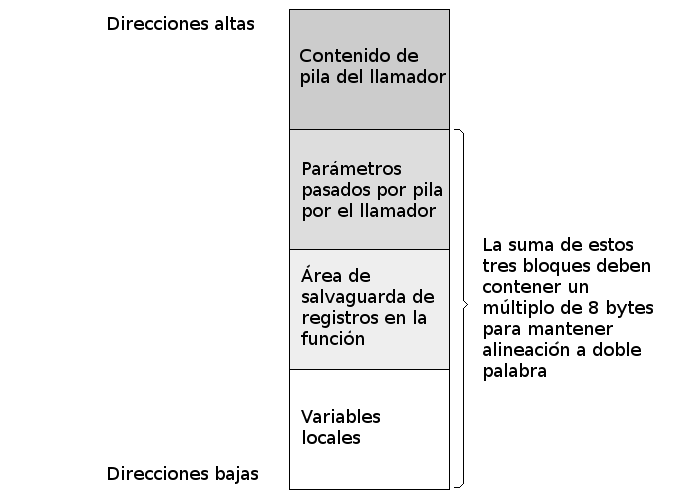
\includegraphics[width=14cm]{graphs/pila.png}
  \caption{Uso de la pila en una función}
  \label{fig:pila}
\end{figure}

Pues bien, en nuestro caso de la función fibonacci necesitamos 0 bytes para paso de parámetros,
4 bytes para salvaguarda de registros (sólo guardaremos {\tt lr}) y 8 bytes para nuestras
dos variables locales. Como la suma es de 12 bytes, que no es múltiplo de 8, redondeamos a 16
añadiendo una tercera variable local que no usaremos (también podríamos haber salvaguardado un
segundo registro).

Nuestro mapa particular lo podemos observar en la figura \ref{fig:pila2}.

\begin{figure}[h]
  \centering
    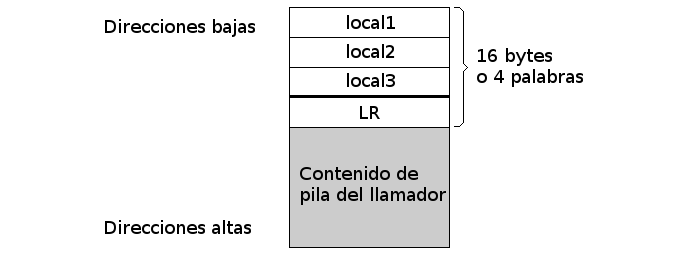
\includegraphics[width=14cm]{graphs/pila2.png}
  \caption{Uso de la pila en nuestra función}
  \label{fig:pila2}
\end{figure}

En teoría podemos encargarnos nosotros mismos de hacer toda la aritmética que conlleva el
uso de variables locales, pero en la práctica estamos más expuestos a cometer errores y
nuestro código es más ilegible. Las 3 variables locales ocupan 12 bytes, a la primera
accedemos con el direccionamiento {\tt [sp]} y a la segunda con {\tt [sp, \#4]} (la tercera
no la usamos). El código quedaría así.

\begin{lstlisting}
fibo:   push    {lr}
        sub     sp, #12
        cmp     r0, #2
        movlo   r0, #1
        blo     fib1
        sub     r0, #1
        str     r0, [sp]
        bl      fibo
        str     r0, [sp, #4]
        ldr     r0, [sp]
        sub     r0, #1
        bl      fibo
        ldr     r1, [sp, #4]
        add     r0, r1
fib1:   add     sp, #12
        pop     {lr}
        bx      lr
\end{lstlisting}

Siguiendo el orden de la pila, primero salvaguardamos {\tt lr} y luego hacemos espacio para
3 palabras con {\tt sub sp, \#12} en el comienzo de la función; al acabar restauramos en orden
inverso, primero restauramos los 12 bytes de las variables locales y luego recuperamos {\tt lr}.

Nuestra función tiene dos ramas, en una se comprueba que el parámetro sea menor de 2, y si lo
es devolvemos el valor 1 y salimos de la función. En la otra rama invocamos nuestra propia
función recursivamente dos veces, sumamos el resultado y devolvemos la suma al salir de la
función.

El truco para hacer el código más legible es nombrando las 3 variables locales y la longitud
mediante la directiva {\tt .equ} (también nos valdría su alias {\tt .set}). Partimos del valor
0 de desplazamiento en la primera variable local y vamos encadenando, a cada elemento le
corresponde la longitud más la posición del anterior. Así, si necesitamos modificar alguna
variable tan sólo tendremos en cuenta la anterior y la siguiente, no tenemos que modificar
toda la estructura.

\begin{lstlisting}
        .equ    local1,   0
        .equ    local2,   4+local1
        .equ    local3,   4+local2
        .equ    length,   4+local3
\end{lstlisting}

Con esta nueva filosofía el código queda menos críptico.

\begin{lstlisting}
fibo:   push    {lr}
        sub     sp, #length
        cmp     r0, #2
        movlo   r0, #1
        blo     fib1
        sub     r0, #1
        str     r0, [sp, #local1]
        bl      fibo
        str     r0, [sp, #local2]
        ldr     r0, [sp, #local1]
        sub     r0, #1
        bl      fibo
        ldr     r1, [sp, #local2]
        add     r0, r1
fib1:   add     sp, #length
        pop     {lr}
        bx      lr
\end{lstlisting}

Ya estamos en condiciones de mostrar el archivo completo.

\begin{lstlisting}[caption={Código del programa subrut3.s},label={lst:codigoPract3_5},escapeinside={@}{@}]
.data
var1:   .asciz  "%d\n"

.text
.global main
main:   push    {r4, lr}
        mov     r4, #0
bucle:  mov     r0, r4
        bl      fibo
        mov     r1, r0
        ldr     r0, =var1
        bl      printf
        add     r4, r4, #1
        cmp     r4, #10
        bne     bucle
        pop     {r4, lr}
        bx      lr

        .equ    local1,   0
        .equ    local2,   4+local1
        .equ    local3,   4+local2
        .equ    length,   4+local3

fibo:   push    {lr}
        sub     sp, #length
        cmp     r0, #2
        movlo   r0, #1
        blo     fib1
        sub     r0, #1
        str     r0, [sp, #local1]
        bl      fibo
        str     r0, [sp, #local2]
        ldr     r0, [sp, #local1]
        sub     r0, #1
        bl      fibo
        ldr     r1, [sp, #local2]
        add     r0, r1
fib1:   add     sp, #length
        pop     {lr}
        bx      lr
\end{lstlisting}

Lo único que nos faltaba era la función {\tt main}. La lista de {\tt .equ} puede
ir al comienzo, pero por claridad la ponemos justo antes de la función a la que
se va a aplicar. La función {\tt main} no tiene nada nuevo, lo único es que incrementamos
el contador {\tt r4} en lugar de decrementar porque lo necesitamos dicho valor como
parámetro para llamar a la función {\tt fibo}.

Para terminar con este ejemplo vamos a hacer una sencilla optimización. Observa un momento
la primera rama de la función. Si el parámetro es menor de dos tan sólo operamos con
un registro, {\tt r0}, tanto para comparar la entrada como para escribir el valor de retorno.
No se toca ningún registro más, no hemos modificado {\tt lr} porque no hemos llamado a ninguna
subrutina, tampoco hemos hecho uso de las variables locales.

La optimización consiste en procesar la primera rama antes de las operaciones con la pila,
de esta forma nos ahorramos algunos ciclos de reloj. Es un buen ejemplo para comprobar
lo flexibles que pueden ser las funciones: hay funciones en las que podemos evitar tratar
con la pila como en el listado \ref{lst:codigoPract3_3}, otras en las que no tenemos más
remedio, y un último caso en que podemos tener una mezcla de ambas.

\begin{lstlisting}[caption={Parte del código del programa subrut4.s},label={lst:codigoPract3_6},escapeinside={@}{@}]
fibo:   cmp     r0, #2
        movlo   r0, #1
        bxlo    lr
        push    {lr}
        sub     sp, #length
        sub     r0, #1
        str     r0, [sp, #local1]
        bl      fibo
        str     r0, [sp, #local2]
        ldr     r0, [sp, #local1]
        sub     r0, #1
        bl      fibo
        ldr     r1, [sp, #local2]
        add     r0, r1
        add     sp, #length
        pop     {lr}
        bx      lr
\end{lstlisting}

\subsection{Funciones con muchos parámetros de entrada}

Lo último que nos falta por ver es cómo acceder a los parámetros de una función por pila, para
lo cual necesitamos una función de al menos cinco parámetros. Lo más sencillo que se nos ocurre
es un algoritmo que evalue cualquier polinomio de grado 3 en el dominio de los enteros.


\begin{equation}
f(x) = ax^3 + bx^2 + cx + d
\label{eq:polinomio}
\end{equation}


Nuestra función tendría 5 entradas, una para cada coeficiente, más el valor de la $x$ que
sería el quinto parámetro que pasamos por pila.

Como siempre, comenzamos escribiendo el código en C.

\begin{lstlisting}[caption={Evaluador de polinomios subrut5.c},label={lst:codigoPract3_6},escapeinside={@}{@}]
int poly3(int a, int b, int c, int d, int x){
  return a*x*x*x + b*x*x + c*x + d;
}

void main(void){
  printf("%d\n%d\n%d\n",
          poly3(1, 2, 3, 4, 5), 
          poly3(1, -1, 1, -1, 8), 
          poly3(2, 0, 0, 0, 8));
}
\end{lstlisting}

Cuya salida es la siguiente.

\begin{lstlisting}
194
455
1024
\end{lstlisting}

El código completo es el siguiente.

\begin{lstlisting}[caption={Evaluador de polinomios subrut5.s},label={lst:codigoPract3_7},escapeinside={@}{@}]
.data
var1:   .asciz  "%d\n"

.text
.global main
main:   push    {r4, lr}
        mov     r0, #1
        mov     r1, #2
        mov     r2, #3
        mov     r3, #4
        mov     r4, #5
        push    {r4}
        bl      poly3
        add     sp, #4
        mov     r1, r0
        ldr     r0, =var1
        bl      printf

        mov     r0, #1
        mov     r1, #-1
        mov     r2, #1
        mov     r3, #-1
        mov     r4, #8
        push    {r4}
        bl      poly3
        add     sp, #4
        mov     r1, r0
        ldr     r0, =var1
        bl      printf

        mov     r0, #2
        mov     r1, #0
        mov     r2, #0
        mov     r3, #0
        mov     r4, #8
        push    {r4}
        bl      poly3
        add     sp, #4
        mov     r1, r0
        ldr     r0, =var1
        bl      printf
        pop     {r4, lr}
        bx      lr

        .equ    param5,   4*1  /* r4 */

poly3:  push    {r4}
        ldr     r4, [sp, #param5]
        smlabb  r3, r2, r4, r3
        smulbb  r2, r4, r4
        smlabb  r3, r1, r2, r3
        smulbb  r2, r2, r4
        smlabb  r0, r0, r2, r3
        pop     {r4}
        bx      lr
\end{lstlisting}

Vemos como hemos usado un {\tt .equ} para facilitar la legibilidad del código, así
accedemos al índice del quinto parámetro sin tener que hacer cálculos. El mapa de la
pila quedaría así.

\begin{figure}[h]
  \centering
    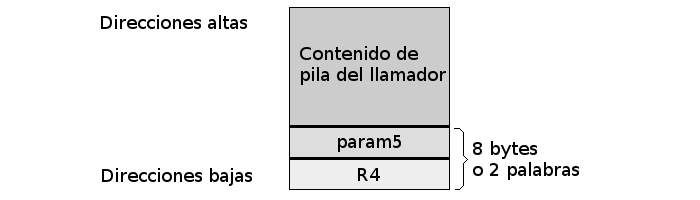
\includegraphics[width=14cm]{graphs/pila3.png}
  \caption{Mapa de pila de función poly3}
  \label{fig:pila3}
\end{figure}

Se pueden combinar los {\tt .equ} de variables locales con los de parámetros por pila,
por ejemplo si tuviésemos una función hipotética con 6 parámetros (dos de ellos pasados
por pila), 3 variables locales y salvaguarda de 3 registros, lo haríamos de la
siguiente forma.

\begin{lstlisting}
      .equ    local1,   0
      .equ    local2,   4+local1
      .equ    local3,   4+local2
      .equ    length,   4+local3
      .equ    param5,   4*3+length /* r4,r5,lr */
      .equ    param6,   4+param5*3

func: push    {r4, r5, lr}
      ...
\end{lstlisting}

Y éste sería el mapa de pila de nuestra hipotética función.

\begin{figure}[h]
  \centering
    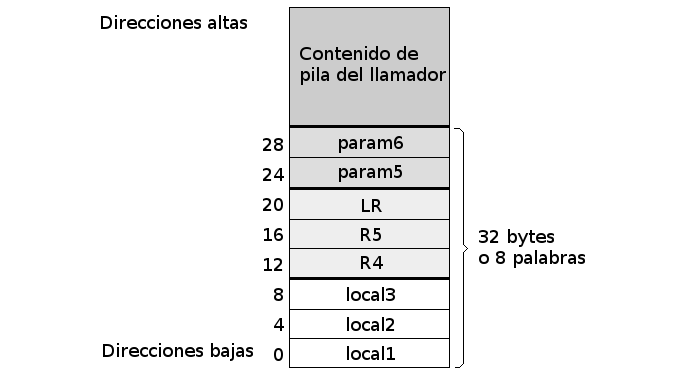
\includegraphics[width=14cm]{graphs/pila4.png}
  \caption{Mapa de función hipotética}
  \label{fig:pila4}
\end{figure}

Los números que hemos puesto números a la izquierda de cada elemento se
corresponden con las constantes que calcula el preprocesador para el
desplazamiento respecto al puntero de pila. De no haber empleado la lista
de {\tt .equ} tendríamos que calcular nosotros mismos estos desplazamientos,
y lo que es peor, el código perdería legibilidad. No es lo mismo poner
{\tt ldr r4, [sp, \#param5]}, que por ejemplo {\tt ldr r4, [sp, \#24]}, habría
que revisar a qué corresponde el desplazamiento {\tt \#24} o indicarlo como
comentario.

Por norma general en la arquitectura ARM se emplean muy poco las variables
locales, ya que operar con éstas implica guardarlas y restaurarlas de memoria,
para lo que se requieren instrucciones adicionales (recuerda que el procesador
no realiza operaciones aritméticas directamente en memoria). En lugar de
variables locales se suelen emplear directamente los registros que han sido
salvaguardados previamente con la instrucción {\tt push}, esto nos da juego
para trabajar con hasta 10 registros (desde {\tt r4} hasta {\tt r12},
incluyendo {\tt lr}) como almacén temporal para nuestras operaciones.

Veamos ahora nuestra función {\tt poly3}. Hemos salvaguardado {\tt r4} porque
necesitamos un almacén temporal donde operar con el quinto parámetro que
leeremos por pila. En esta función la pila está alineada a 8 bytes porque
usamos 4 bytes en el quinto parámetro más los 4 bytes de salvaguardar {\tt r4},
en total 8 bytes.

Todas los cálculos se condensan en 5 líneas donde se alternan las instrucciones
{\tt smlaxy} y {\tt smulxy}. Son instrucciones que multiplican/acumulan y
multiplican respectivamente números enteros. El comportamiento exacto de cada
instrucción viene detallado en el datasheet del procesador, aunque funciona
bastante bien buscándolas en google, suele aparecer la ayuda oficial en el primer
resultado de la búsqueda.

\begin{lstlisting}
  smlabb  r3, r2, r4, r3 /* r3= d+c*x             */
  smulbb  r2, r4, r4     /* r2= x^2               */
  smlabb  r3, r1, r2, r3 /* r3= d+c*x+b*x^2       */
  smulbb  r2, r2, r4     /* r2= x^3               */
  smlabb  r0, r0, r2, r3 /* r0= d+c*x+b*x^2+a*x^3 */
\end{lstlisting}

Como podéis observar, las instrucciones ARM son muy potentes, permiten
implementar en 5 instrucciones lo que en C nos habría costado 6
multiplicaciones y 4 sumas. Nótese como utilizamos como registros
intermedios {\tt r2, r3} los parámetros de entrada a medida que no los
necesitamos más.

Después de esto acaba la función con las habituales {\tt pop {r4}} y
{\tt bx lr}. Ya hemos terminado la función {\tt poly3}, ha quedado
bastante pequeña en tamaño. Todo lo contrario que la función {\tt main}.

La función {\tt main} es larga por varias razones: hacemos 3 llamadas
a {\tt poly3}, debemos introducir muchas constantes, algunas de ellas
en pila, y debemos imprimir los resultados y hacer el equilibrado de pila.

El equilibrado de pila consiste en incrementar {\tt sp} después de la
llamada a la función para desalojar los parámetros que previamente habíamos
introducido en la misma. Como en nuestro ejemplo pasamos por pila un
único parámetro de 4 bytes, lo que hacemos es incrementar {\tt sp} en 4 tras
cada llamada a {\tt poly3}.

Un detalle muy importante que no podemos observar en nuestro ejemplo, los
parámetros que pasamos por pila lo hacemos en orden inverso desde el último
al quinto. Esto es así porque la pila crece hacia abajo. Es más, es
aconsejable reusar los registros {\tt r0-r3} para introducir los
parámetros por pila. Si tuviésemos que pasar 6 parámetros, constantes del
1 al 6 lo haríamos así.

\begin{lstlisting}
        mov     r0, #6
        push    {r0}
        mov     r0, #5
        push    {r0}
        mov     r0, #1
        mov     r1, #2
        mov     r2, #3
        mov     r3, #4
\end{lstlisting}

Como véis no hay una forma clara y legible de introducir los parámetros
de una función. Tened cuidado con los push múltiples, no importa el orden
en que introduzcas los registros, el procesador siempre introduce en pila
el registro más alto y va hacia atrás hasta llegar al primero. Aprovechando
esto podemos mejorar el ejemplo anterior.

\begin{lstlisting}
        mov     r0, #5
        mov     r1, #6
        push    {r0, r1}
        mov     r0, #1
        mov     r1, #2
        mov     r2, #3
        mov     r3, #4
\end{lstlisting}

Por último vamos a mejorar un poco la velocidad de la función {\tt poly3} de
esta forma.

\begin{lstlisting}[caption={Parte de subrut6.s},label={lst:codigoPract3_8},escapeinside={@}{@}]
poly3:  sub     sp, #4
        ldr     r12, [sp, #param5]
        smlabb  r3, r2, r12, r3
        smulbb  r2, r12, r12
        smlabb  r3, r1, r2, r3
        smulbb  r2, r2, r12
        smlabb  r0, r0, r2, r3
        add     sp, #4
        bx      lr
\end{lstlisting}

¿En qué consiste la mejora? Pues que hemos usado el registro basura {\tt r12}, que
es el único que podemos emplear sin salvaguardarlo previamente en la lista del {\tt push}.
Esto nos quitaría el {\tt push} y el {\tt pop}, aunque en este ejemplo lo hemos
reemplazado por instrucciones {\tt sub} y {\tt add}. La razón es que debemos mantener
el puntero de pila en un múltiplo de 8. No obstante las instrucciones que no acceden
a memoria siempre son más rápidas que las que lo hacen, así que hemos ganado velocidad.

\subsection{Pasos detallados de llamadas a funciones}

Como ya hemos visto todos los casos posibles, hacemos un resumen de todo en una
serie de puntos desde que pasamos los parámetros en el llamador hasta que restauramos
la pila desde el llamador, pasando por la llamada a la función y la ejecución de la misma.

\begin{itemize}
  \item Usamos los registros {\tt r0-r3} como almacén temporal el llamador pasa por pila
        los parámetros quinto, sexto, etc... hasta el último. Cuidado con el orden,
        especialmente si se emplea un {\tt push} múltiple. Opcional, sólo si nuestra
        función tiene más de 4 parámetros.
  \item El llamador escribe los primeros 4 parámetros en {\tt r0-r3}. Opcional, nos
        podemos saltar este paso si nuestra función no tiene parámetros.
  \item El llamador invoca a la función con {\tt bl}. Este paso es obligatorio.
  \item Ya dentro de la función, lo primero que hace esta es salvaguardar los registros
        desde {\tt r4} que se empleen más adelante como registros temporales. También opcional.
  \item Decrementar la pila para hacer hueco a las variables locales. La suma de bytes
        entre paso de parámetros por pila, salvaguarda y variables locales debe ser
        múltiplo de 8, rellenar aquí hasta completar. Como este paso es opcional, en caso
        de no hacerlo aquí rellenar en el paso anterior.
  \item La función realiza las operaciones que necesite para completar su objetivo, accediendo
        a parámetros y variables locales mediante constantes {\tt .equ} para aportar mayor claridad
        al código. Se devuelve el valor resultado en {\tt r0} (ó en {\tt r1:r0} si es doble
        palabra).
  \item Incrementar la pila para revertir el alojamiento de variables locales.
  \item Recuperar con {\tt pop} la lista de registros salvaguardados.
  \item Retornar la función con {\tt bx lr} volviendo al código llamador, exactamente a la
        instrucción que hay tras el {\tt bl}. 
  \item El llamador equilibra la pila en caso de haber pasado parámetros por ella.
\end{itemize}

\section{Ejercicios}

\subsection{Mínimo de un vector}

Dado un vector de enteros y su longitud, escribe una función en ensamblador
que recorra todos los elementos del vector y nos devuelva el valor mínimo.
Para comprobar su funcionamiento, haz {\tt .global} la función y tras ensamblarla,
enlázala con este programa en C.

\begin{lstlisting}
#include <stdio.h>

int vect[]= {8, 10, -3, 4, -5, 50, 2, 3};

void main(void){
  printf("%d\n", minimo(vect, 8));
}
\end{lstlisting}

Hay muchas formas de calcular el mínimo de una lista de elementos, la más sencilla es
comparar todos los elemento con una variable, la cual actualizamos sólo si el elemento es
menor que la variable.

\begin{center}
\begin{myfbox}
\small
\begin{minipage}{0.92\linewidth}
\begin{center}
\begin{minipage}{0.6\linewidth}
\begin{verbatim}
  int minimo(int* v, int len){
    int i, min;

    min= v[0];
    for ( i= 1; i<len; i++ )
      if( v[i]<min )
        min= v[i];
    return min;
  }
\end{verbatim}
\end{minipage}
\end{center}
\begin{center}
\colorbox[gray]{1}{\rule{0cm}{7cm}\rule{11cm}{0cm}}
\end{center}
\end{minipage}
\end{myfbox}
\end{center}

\subsection{Media aritmética, macros y conteo de ciclos}

\subsubsection{Media aritmética}

Escribe una función en ensamblador que calcule la media aritmética (truncada porque
trabajamos con enteros) de dos números. Escribe también la función {\tt main} con 
cinco llamadas a {\tt media} con distintos parámetros.

\begin{center}
\begin{myfbox}
\small
\begin{minipage}{0.92\linewidth}
\begin{center}
\colorbox[gray]{1}{\rule{0cm}{4.5cm}\rule{11cm}{0cm}}
\end{center}
\end{minipage}
\end{myfbox}
\end{center}

Una vez hecho esto, supón que cada instrucción tarda un ciclo de reloj en ejecutarse.
Cuenta manualmente el número de ciclos que tarda la ejecución completa desde la primera
instrucción de {\tt main} hasta la última {\tt bx lr}, incluyendo ésta. En caso de una
llamada a subrutina cuenta todas las instrucciones que se ejecutan metiéndote en la
subrutina. La única excepción es {\tt bl printf}, que debes contar como un único ciclo.

Haz lo mismo pero usando la herramienta {\tt gdb} para comprobar el resultado anterior.
Recuerda no meterte dentro de los printf con {\tt ni}, en las llamadas a la función
{\tt abs} usa {\tt si}.

\subsubsection{Macros}

Hay una forma de acelerar las funciones, aunque sólo es práctica para funciones pequeñas
que se utilicen mucho. Se trata de escribir el contenido de la función en lugar de
llamar a la misma, y para evitar repetir siempre el mismo código utilizamos la directiva
{\tt .macro}. Con este truco nos ahorramos al menos la ejecución de las instrucciones
{\tt bl funcion} y {\tt bx lr}. El inconveniente es que el tamaño del ejecutable será
mayor.

Como ejemplo vamos a dar una implementación del método {\tt abs}.

\begin{lstlisting}[caption={Parte de subrut8.s},label={lst:codigoPract3_9},escapeinside={@}{@}]
      .macro  abs
        tst     r0, r0
        negmi   r0, r0
      .endm

.data
var1:   .asciz  "%d\n"

.text
.global main
main:   push    {r4, lr}
        mov     r0, #1
        bl      abs
        mov     r1, r0
        ldr     r0, =var1
        bl      printf

        mov     r0, #-2
        bl      abs
        mov     r1, r0
        ldr     r0, =var1
        bl      printf

        mov     r0, #3
        bl      abs
        mov     r1, r0
        ldr     r0, =var1
        bl      printf

        mov     r0, #-4
        bl      abs
        mov     r1, r0
        ldr     r0, =var1
        bl      printf
        pop     {r4, lr}
        bx      lr

abs:    tst     r0, r0
        negmi   r0, r0
        bx      lr
\end{lstlisting}

Borra el {\tt bl} antes del {\tt abs} para probar la versión con macros. Dentro de 
{\tt gdb} la secuencia de comandos para contar los pasos saltándose el
{\tt bl printf} junto con la cuenta es la siguiente.

\begin{lstlisting}
start / si 6 / ni / si 5 / ni /
/ si 5 / ni / si 5 / ni / si 2
6+1+(5+1)*3+2 = 27
\end{lstlisting}

Reescribe el ejercicio anterior de la media aritmética empleando macros en vez de
funciones.

\subsubsection{Conteo de ciclos}

Completa la siguiente tabla usando los dos tipos de conteo que acabamos de explicar.

\begin{center}
\small
\colorbox[gray]{0.9}{
%\arrayrulecolor{black}
\tabcolsep = 1mm
\begin{tabular}{ccccc}
&Ciclos contados & Ciclos contados & Ciclos manualmente & Ciclos, con {\tt gdb} \\
&manualmente & con {\tt gdb}       & empleando macros & y macros \\
media &
\colorbox[gray]{1}{\rule{0cm}{0.46cm}\rule{2.6cm}{0cm}} &
\colorbox[gray]{1}{\rule{0cm}{0.46cm}\rule{2.6cm}{0cm}} &
\colorbox[gray]{1}{\rule{0cm}{0.46cm}\rule{2.6cm}{0cm}} &
\colorbox[gray]{1}{\rule{0cm}{0.46cm}\rule{2.6cm}{0cm}} \\[1mm]
abs &
\colorbox[gray]{1}{\rule{0cm}{0.46cm}\rule{2.6cm}{0cm}} &
\colorbox[gray]{1}{\rule{0cm}{0.46cm}\rule{2.6cm}{0cm}} &
\colorbox[gray]{1}{\rule{0cm}{0.46cm}\rule{2.6cm}{0cm}} &
\colorbox[gray]{1}{\rule{0cm}{0.46cm}\rule{1.1cm}{0cm}27\rule{1.1cm}{0cm}} \\
\end{tabular}
\vspace{0.5ex}
}
\end{center}

Este conteo de ciclos es ilustrativo. En un procesador real sólo
las instrucciones simples tardan un ciclo de reloj, siempre y cuando
el resultado de la operación no se utilice en la instrucción posterior,
en cuyo la duración es de dos ciclos. Después hay instrucciones
complejas como las multiplicaciones, que necesitan 3 ciclos (más si hay
que añadir la penalización anterior). Por último están los casos 
más complejos. Por un lado tenemos los saltos condicionales, donde el
procesador hace una predicción de salto dentro de las 2 posibilidades
que hay, si se produce un fallo en la predicción se penalizan ciclos.
Por otro lado están los accesos a memoria, que tampoco tienen una
temporización constante porque está la caché por medio. Si se produce
un fallo de caché hay que añadir la penalización correspondiente.

\subsection{Algoritmo de ordenación}

Escoge un algoritmo de ordenación de entre los 4 siguientes.

\begin{itemize}
  \item Burbuja.
  \item Selección.
  \item Inserción.
  \item Quicksort.
\end{itemize}

E impleméntalo en ensamblador. Como ejemplo mostramos el código en C
del algoritmo de la burbuja.

\begin{lstlisting}[caption={Parte de subrut9.c},label={lst:codigoPract3_10},escapeinside={@}{@}]
#include <stdio.h>

int vect[]= {8, 10, -3, 4, -5, 50, 2, 3};

void ordena(int* v, int len){
  int i, j, aux;

  for ( i= 1; i<len; i++ )
    for ( j= 0; j<len-i; j++ )
      if( v[j] > v[j+1] )
        aux= v[j],
        v[j]= v[j+1],
        v[j+1]= aux;
}

void main(void){
  int i;

  ordena(vect, 8);
  for ( i= 0; i<8; i++ )
    printf("%d\n", vect[i]);
}
\end{lstlisting}

La lista de algoritmos está ordenada por dificultad, por lo que el algoritmo
{\tt Quicksort} es con diferencia el más difícil de implementar. Recomendamos
dejarlo para el final en caso de que el alumno decida realizar los 4 algoritmos
en ensamblador.

\chapterend{}

%%%%%%%%%%%%%%%%%%%%%%%%%%%%%%%%%%%%%%%%%%%%%%%%%%%%%%%%%%%%%%
\end{document}

% Capítulo 04.
\chapterbegin{E/S a bajo nivel}
\label{chp:Subrut}
\minitoc

{\bf Objetivos}: Hasta ahora hemos programado en ensamblador sobre
la capa que nos ofrece el sistema operativo. Nosotros llamamos a una
función y ésta hace todo lo demás: le dice al sistema operativo lo
que tiene que hacer con tal periférico y el sistema operativo (en concreto
el kernel) le envía las órdenes directamente al periférico, al espacio
de memoria donde esté mapeado el mismo.

Lo que vamos a hacer en este capítulo es comunicarnos directamente con los
periféricos, para lo cual debemos prescindir totalmente del sistema operativo.
Este modo de acceder directamente al hardware de la máquina se denomina {\tt Bare Metal},
que traducido viene a ser algo como {\tt Metal desnudo}, haciendo referencia a
que estamos ante la máquina tal y cómo es, sin ninguna capa de abstracción de
por medio.

Veremos ejemplos de acceso directo a periféricos, en concreto al LED de la placa
auxiliar (ver apéndice \ref{chp:PlacaAux}) y a los temporizadores, que son
bastante sencillos de manejar.

\section{Lectura previa}

\subsection{Librerías y Kernel, las dos capas que queremos saltarnos}

Anteriormente hemos utilizado funciones específicas para
comunicarnos con los periféricos. Si por ejemplo necesitamos escribir
en pantalla, llamamos a la función {\tt printf}. Pues bien, entre
la llamada a la función y lo que vemos en pantalla hay 2 capas software
de por medio.

Una primera capa se encuentra en la librería runtime que acompaña al
ejecutable, la cual incluye sólamente el fragmento de código de la
función que necesitemos, en este caso en {\tt printf}. El resto de
funciones de la librería ({\tt stdio}), si no las invocamos no aparecen
en el ejecutable. El enlazador se encarga de todo esto, tanto de ubicar
las funciones que llamemos desde ensamblador, como de poner la dirección
numérica correcta que corresponda en la instrucción {\tt bl printf}.

Este fragmento de código perteneciente a la primera capa sí que podemos
depurarlo mediante {\tt gdb}. Lo que hace es, a parte del formateo que
realiza la propia función, trasladar al sistema operativo una determinada
cadena para que éste lo muestre por pantalla. Es una especie de traductor
intermedio que nos facilita las cosas. Nosotros desde ensamblador también
podemos hacer llamadas al sistema directamente como veremos posteriormente.

La segunda capa va desde que hacemos la llamada al sistema hasta que se
produce la transferencia de datos al periférico, retornando desde la llamada
al sistema y volviendo a la primera capa, que a su vez retornará el control
a la llamada a librería que hicimos en nuestro programa inicialmente.

En esta segunda capa se ejecuta código del kernel, el cual no podemos depurar.
Además el procesador entra en un modo privilegiado, ya que en modo usuario (el
que se ejecuta en nuestro programa ensamblador y dentro de la librería) no
tenemos privilegios suficientes como para acceder a la zona de memoria que
mapea los periféricos.

En la figura \ref{fig:capas} podemos ver el código llamador junto con las dos
capas.

\begin{figure}[h]
  \centering
    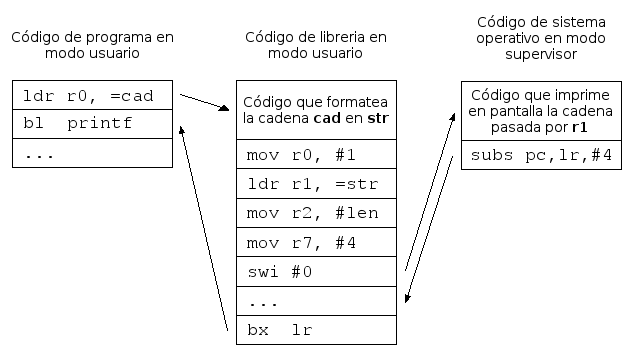
\includegraphics[width=14cm]{graphs/capas.png}
  \caption{Funcionamiento de una llamada a printf}
  \label{fig:capas}
\end{figure}

Ahora veremos un ejemplo en el cual nos saltamos la capa intermedia para
comunicarnos directamente con el kernel vía llamada al sistema. En este ejemplo
vamos a escribir una simple cadena por pantalla, en concreto "Hola Mundo!".

\begin{lstlisting}[caption={esbn1.s},label={lst:codigoPract4_1},escapeinside={@}{@}]
.data

cadena: .asciz "Hola Mundo!\n"
cadenafin:

.text
.global main
 
main:   push    {r7, lr}           /* preservamos reg.*/
        mov     r0, #1             /* salida estándar */
        ldr     r1, =cadena        /* cadena a enviar */
        mov     r2, #cadenafin-cadena     /* longitud */
        mov     r7, #4             /* seleccionamos la*/
        swi     #0        /* llamada a sistema 'write'*/
        mov     r0, #0             /* devolvemos ok   */
        pop     {r7, lr}           /* recuperamos reg.*/
        bx      lr                 /* salimos de main */
\end{lstlisting}

La instrucción que ejecuta la llamada al sistema es {\tt swi \#0},
siempre tendrá cero como valor inmediato. El código numérico de
la llamada y el número de parámetros podemos buscarlo en cualquier
manual de Linux, buscando ``Linux system call table'' en Google. En
nuestro caso la llamada {\tt write} se corresponde con el código
4 y acepta tres parámetros: manejador de fichero, dirección de
los datos a escribir (nuestra cadena) y longitud de los datos.

En general se tiende a usar una lista reducida de posibles llamadas
a sistema, y que éstas sean lo más polivalentes posibles. En este
caso vemos que no existe una función específica para escribir en
pantalla. Lo que hacemos es escribir bytes en un fichero, pero usando
un manejador especial conocido como salida estándar, con lo cual todo
lo que escribamos a este fichero especial aparecerá por pantalla.

Pero el propósito de este capítulo no es saltarnos una capa
para comunicarnos directamente con el sistema operativo. Lo que queremos
es saltarnos las dos capas y enviarle órdenes directamente a los periféricos.
Para esto tenemos prescindir del sistema operativo, o lo que es lo mismo,
hacer nosotros de sistema operativo para realizar las tareas que queramos.

Este modo de trabajar (como hemos adelantado) se denomina Bare Metal, porque
accedemos a las entrañas del hardware. En él podemos hacer desde cosas
muy sencillas como encender un LED hasta programar desde cero nuestro propio
sistema operativo.

\subsection{Ejecutar código en Bare Metal}

El ciclo de ensamblado y enlazado es distinto en un programa Bare Metal. Hasta
ahora hemos creado ejecutables, que tienen una estructura más compleja, con cabecera y
distintas secciones en formato {\tt ELF}. Toda esta información le viene muy bien al
sistema operativo, pero en un entorno Bare Metal no disponemos de él. Lo que se carga
en {\tt kernel.img} es un binario sencillo, sin cabecera, que contiene directamente
el código máquina de nuestro programa y que se cargará en la dirección de RAM {\tt 0x8000}.

Lo que para un ejecutable hacíamos con esta secuencia.
\begin{lstlisting}
        as -o ejemplo.o ejemplo.s
        gcc -o ejemplo ejemplo.o
\end{lstlisting}

En caso de un programa Bare Metal tenemos que cambiarla por esta otra.
\begin{lstlisting}
        as -o ejemplo.o ejemplo.s
        ld -e 0 -Ttext=0x8000 -o ejemplo.elf ejemplo.o
        objcopy ejemplo.elf -O binary kernel.img
\end{lstlisting}

Otra característica de Bare Metal es que sólo tenemos una sección de código (la sección
.text), y no estamos obligados a crear la función
{\tt main}. Al no ejecutar ninguna función no tenemos la posibilidad de salir del
programa con {\tt bx lr}, al fin y al cabo no hay ningún sistema operativo detrás al
que regresar. Nuestro programa debe trabajar en bucle cerrado. En caso de tener una
tarea simple que querramos terminar, es preferible dejar el sistema colgado con un
bucle infinito como última instrucción.

El proceso de arranque de la Raspberry Pi es el siguiente:

\begin{itemize}
  \item Cuando la encendemos, el núcleo ARM está desactivado. Lo primero que se activa es el
        núcleo GPU, que es un procesador totalmente distinto e independiente al ARM. En este
        momento la SDRAM está desactivada.
  \item El procesador GPU empieza a ejecutar la primera etapa del bootloader (son 3 etapas), que
        está almacenada en ROM dentro del mismo chip que comparten ARM y GPU. Esta primera etapa
        accede a la tarjeta SD y lee el fichero {\tt bootcode.bin} en caché L2 y lo ejecuta,
        siendo el código de {\tt bootcode.bin} la segunda etapa del bootloader.
  \item En la segunda etapa se activa la SDRAM y se carga la tercera parte del bootloader, cuyo
        código está repartido entre {\tt loader.bin} (opcional) y {\tt start.elf}.
  \item En tercera y última etapa del bootloader se accede opcionalmente a dos archivos ASCII de
        configuración llamados {\tt config.txt} y {\tt cmdline.txt}. Lo más relevante de esta
        etapa es que cargamos en RAM (en concreto en la dirección 0x8000) el archivo
        {\tt kernel.img} con código ARM, para luego ejecutarlo y acabar con el bootloader, pasando
        el control desde la GPU hacia la CPU.
        Este último archivo es el que nos interesa modificar para nuestros propósitos, ya que es
        lo primero que la CPU ejecuta y lo hace en modo privilegiado, es decir, con acceso total
        al hardware.
\end{itemize}

De todos estos archivos los obligatorios son {\tt bootcode.bin}, {\tt start.elf} y
{\tt kernel.img}. Los dos primeros los bajamos del repositorio oficial
\textcolor{blue}{
  \href{https://github.com/raspberrypi}
  {https://github.com/raspberrypi}}
y el tercero {\tt kernel.img} es el que nosotros
vamos a generar. Estos tres archivos deben estar en el directorio raíz de la primera partición
de la tarjeta SD, la cual debe estar formateada en FAT32.

El proceso completo que debemos repetir cada vez que desarrollemos un programa nuevo
en Bare Metal es el siguiente:

\begin{itemize}
  \item Apagamos la Raspberry.
  \item Extraemos la tarjeta SD.
  \item Introducimos la SD en el lector de nuestro ordenador de desarrollo.
  \item Montamos la unidad y copiamos (sobreescribimos) el kernel.img que acabamos
        de desarrollar.
  \item Desmontamos y extraemos la SD.
  \item Insertamos de nuevo la SD en la Raspberry y la encendemos.
\end{itemize}

Es un proceso sencillo para las prácticas que vamos a hacer, pero para proyectos más largos
se vuelve bastante pesado de realizar. Hay varias alternativas que agilizan el ciclo de
trabajo, donde no es necesario extraer la SD y por tanto podemos actualizar el {\tt kernel.img}
en cuestión de segundos.

\begin{itemize}
  \item Cable JTAG con software Openocd
\textcolor{blue}{
  \href{http://openocd.sourceforge.net}
  {http://openocd.sourceforge.net}}
  \item Cable USB-serie desde el ordenador de desarrollo hacia la Raspberry, requiere
        tener instaladas las herramientas de compilación cruzada en el ordenador de desarrollo.
  \item Cable serie-serie que comunica dos Raspberries, una orientada a desarrollo y la otra
        para ejecutar los programas en Bare Metal. No es imprescindible trabajar directamente
        con la Raspberry de desarrollo, podemos acceder vía ssh con nuestro ordenador habitual,
        sin necesidad de tener instaladas las herramientas de compilación en el mismo.
\end{itemize}

Las dos últimas opciones están detalladas en el apéndice \ref{chp:SerieBoot},
básicamente se trata de meter en el kernel.img de la SD un programa especial (llamado
bootloader) que lee continuamente del puerto serie y en el momento en que recibe
un archivo lo carga en RAM y lo ejecuta.

\section{Acceso a periféricos}

Los periféricos se controlan leyendo y escribiendo datos a los registros asociados. No
confundir estos registros con los registros de la CPU. Un registro asociado a un periférico
es un ente, normalmente del mismo tamaño que el ancho del bus de datos, que sirve para
configurar diferentes aspectos del mismo. No se trata de RAM, por lo que no se garantiza que
al leer de un registro obtengamos el último valor que escribimos. Es más, incluso hay
registros que sólo admiten ser leídos y otros que sólo admiten escrituras. La funcionalidad
de los registros también es muy variable, incluso dentro de un mismo registro los diferentes
bits del mismo tienen distinto comportamiento.

Como cada periférico se controla de una forma diferente, no hay más remedio que leerse
el datasheet del mismo si queremos trabajar con él. En nuestro caso queremos encender un LED
en la placa auxiliar, que conectaremos a la fila inferior del conector GPIO según la
figura \ref{fig:posicionaux}.

\begin{figure}[h]
  \centering
    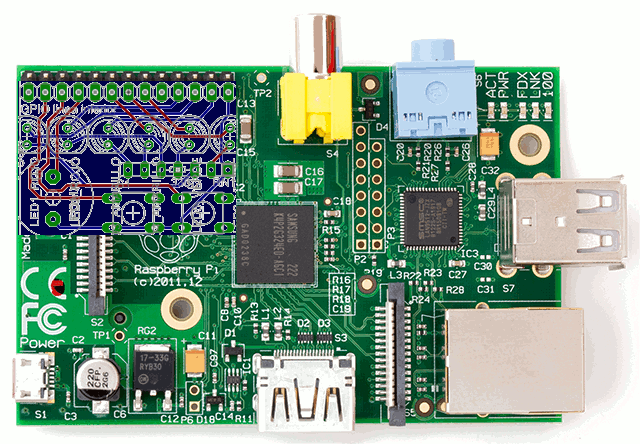
\includegraphics[width=14cm]{graphs/posicionaux.png}
  \caption{Colocación de la placa auxiliar}
  \label{fig:posicionaux}
\end{figure}


\subsection{GPIO}

GPIO es un conjunto de señales mediante las cuales la CPU se comunica con distintas partes
de la Rasberry tanto internamente (audio analógico, tarjeta SD o LEDs internos) como
externamente a través de los conectores P1 y P5. Como la mayor parte de las señales se
encuentran en el conector P1, normalmente este conector se denomina GPIO. Nosotros
no vamos a trabajar con señales GPIO que no pertenezcan a dicho conector, por lo que no
habrá confusiones.

En total son 54 señales, de las cuales 17 están disponibles a través del conector
GPIO (26 en los modelos A+/B+). Como nuestra placa auxiliar emplea la fila inferior
del conector, sólo dispondremos de 9 señales.

Los registros del GPIO están mapeados en memoria, tomando como base la dirección 0x20200000.
Para nuestros propósitos de esta lección nos basta con acceder a los registros GPFSELn,
GPSETn y GPCLRn. A continuación tenemos la tabla con las direcciones de estos registros.

\begin{table}
\centering
\begin{tabular}{ p{1.8cm} | p{2cm} | p{5cm} | p{1cm} }
{\bf Dirección} & {\bf Nombre} & {\bf Descripción} & {\bf Tipo} \\
\hline
20200000 & GPFSEL0 & Selector de función 0 & R/W \\
20200004 & GPFSEL1 & Selector de función 1 & R/W \\
20200008 & GPFSEL2 & Selector de función 2 & R/W \\
2020000C & GPFSEL3 & Selector de función 3 & R/W \\
20200010 & GPFSEL4 & Selector de función 4 & R/W \\
20200014 & GPFSEL5 & Selector de función 5 & R/W \\
2020001C & GPSET0  & Pin a nivel alto 0 & W   \\
20200020 & GPSET1  & Pin a nivel alto 1 & W   \\
20200028 & GPCLR0  & Pin a nivel bajo 0 & W  \\
2020002C & GPCLR1  & Pin a nivel bajo 1 & W  \\
\end{tabular}
\end{table}


\subsubsection{GPFSELn}

Las 54 señales las separamos en 6
grupos funcionales de 10 pines cada uno (excepto el último
que es de 4) para programarlas mediante GPFSELn.

El LED que queremos controlar se corresponde con la señal número 9 del puerto GPIO.
Se nombran con GPIO más el número correspondiente, en nuestro caso sería GPIO 9. Nótese
que la numeración empieza en 0, desde GPIO 0 hasta GPIO 53.

Así que la funcionalidad desde GPIO 0 hasta GPIO 9 se controla con
GPFSEL0, desde GPIO 10 hasta GPIO 19 se hace con GPFSEL1 y así
sucesivamente. Nosotros queremos cambiar la funcionalidad de GPIO 9
que está en GPFSEL0. Por defecto cuando arranca la Raspberry
todos los pines están preconfigurados como entradas, con lo que los LEDs
están apagados. Es más, aunque lo configuremos como salida, tras el reset
parten del valor cero (nivel bajo), por lo que podemos presuponer que
todos los LEDs estarán apagados, incluso después de programarlos como salidas.

El registro GPFSEL0 contiene diez grupos funcionales
llamados FSELx (del 0 al 9) de 3 bits cada uno, quedando los dos bits
más altos sin usar. Nos interesa cambiar FSEL9, que sería el que se corresponde
con el LED rojo de más a la izquierda, el que queremos encender. Las posibles
configuraciones para cada grupo son:

\begin{lstlisting}
000 = GPIO Pin X es una entrada
001 = GPIO Pin X es una salida
100 = GPIO Pin X toma función alternativa 0
101 = GPIO Pin X toma función alternativa 1
110 = GPIO Pin X toma función alternativa 2
111 = GPIO Pin X toma función alternativa 3
011 = GPIO Pin X toma función alternativa 4
010 = GPIO Pin X toma función alternativa 5
\end{lstlisting}

Las funciones alternativas son para dotar a los pines de funcionalidad específicas
como puertos SPI, UART, audio PCM y cosas parecidas. La lista completa
está en la tabla 6-31 (página 102) del datasheet. Nosotros queremos una salida
genérica, nos quedamos con el código {\tt 001}.


\subsubsection{GPSETn y GPCLRn}

Una vez configurado GPIO 9 como salida, ya sólo queda saber cómo poner un cero o un
uno en la señal GPIO 9, para apagar y encender el primer LED respectivamente (un cero apaga
y un uno enciende el LED).

Para ello tenemos los registros GPSETn y GPCLRn. En principio parece enrevesado el tener
que usar dos registros distintos para escribir en el puerto GPIO, pero no olvidemos que
para ahorrar recursos varios pines están empaquetados en una palabra de 32 bits. Por lo
que si quisiéramos alterar un único pin tendríamos que leer el registro, modificar el bit
en cuestión sin tocar los demás y escribir el resultado de nuevo en el registro. Por suerte
esto no es necesario con registros separados para setear y resetear, tan sólo necesitamos
una escritura en registro poniendo a 1 los bits que queramos setear/resetear y a 0 los bits
que no queramos modificar.

En la figura \ref{fig:pinout} vemos cómo está hecho el conexionado de la placa auxiliar.

\begin{figure}[h]
  \centering
    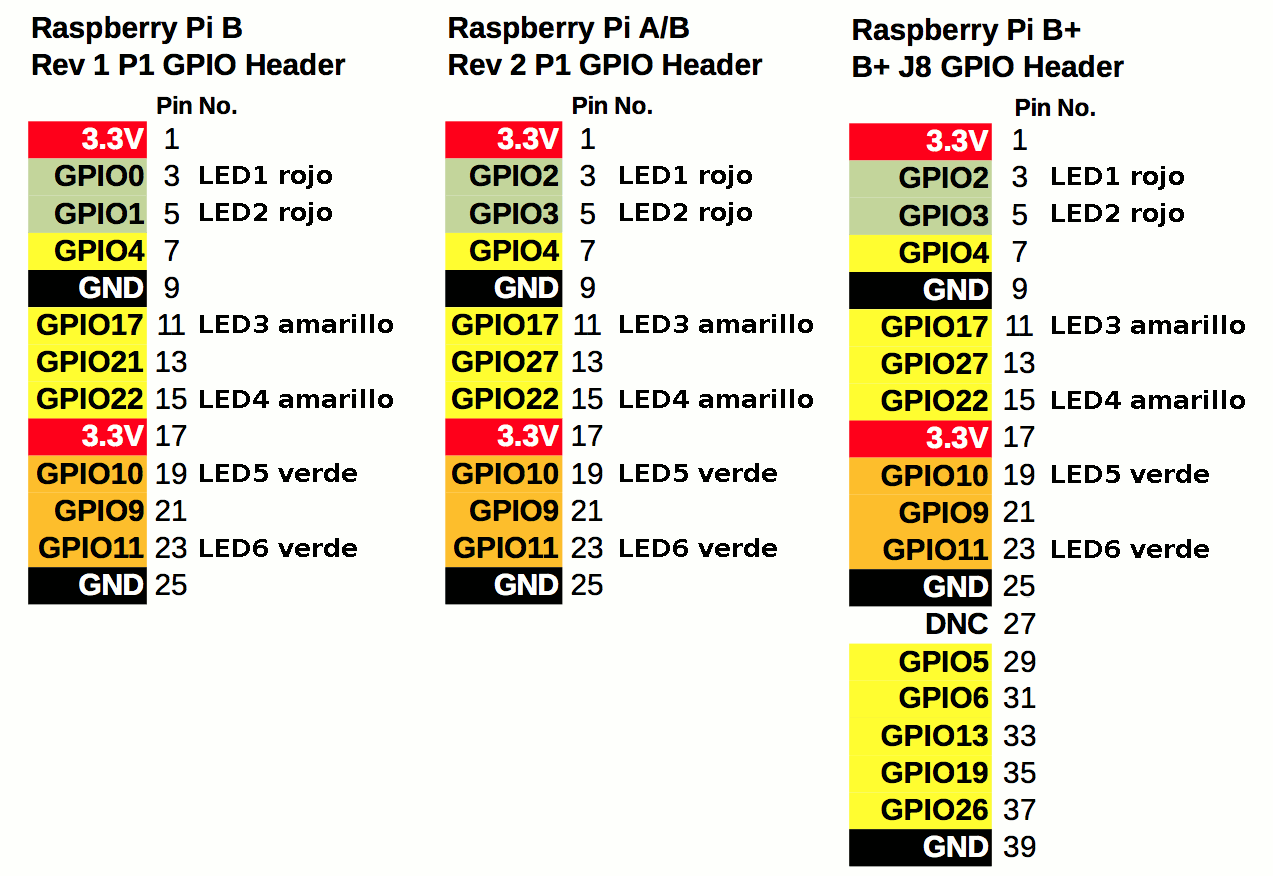
\includegraphics[width=14cm]{graphs/RaspberryGPIOaux.png}
  \caption{Correspondencia LEDs y GPIO}
  \label{fig:pinout}
\end{figure}

Leemos el datasheet y comprobamos que es así. Además los 54 pines se reparten entre dos
registros GPSET0/GPCLR0, que contienen los 32 primeros, y en GPSET1/GPCLR1 están los 22
restantes, quedando libres los 10 bits más significativos de GPSET1/GPCLR1.

En nuestro
primer ejemplo de Bare Metal sólo vamos a encender el primer LED de la placa auxiliar,
por lo que emplearemos el registro GPCLR0.

\begin{lstlisting}[caption={esbn2.s},label={lst:codigoPract4_2}]
        .set    GPBASE,   0x20200000
        .set    GPFSEL0,  0x00
        .set    GPSET0,   0x1c
.text
        ldr     r0, =GPBASE
        mov     r1, #0b00001000000000000000000000000000
/* guia bits           xx999888777666555444333222111000*/
        str     r1, [r0, #GPFSEL0]
/* guia bits           10987654321098765432109876543210*/
        mov     r1, #0b00000000000000000000001000000000
        str     r1, [r0, #GPSET0]
infi:   b       infi
\end{lstlisting}

El acceso a los registros lo hemos hecho usando la dirección base donde
están mapeados los periféricos {\tt 0x20200000}. Cargamos esta dirección
base en el registro {\tt r0} y codificamos los accesos a los registros
E/S con direccionamiento a memoria empleando distintas constantes como
desplazamiento en función del registro al que queramos acceder.

Los registros a los que accedemos para encender y apagar el LED vienen indicados
en la figura \ref{fig:gpio1}.

\begin{figure}[h]
  \centering
    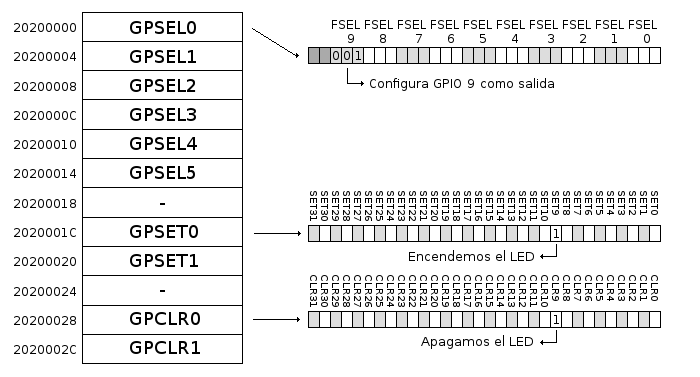
\includegraphics[width=14cm]{graphs/gpio1.png}
  \caption{Registros LED}
  \label{fig:gpio1}
\end{figure}

El código simplemente escribe dos constantes en dos registros: {\tt GPFSEL0} y {\tt GPSET0}.
Con la primera escritura configuramos el LED como salida y con la segunda escritura lo
encendemos, para finalmente entrar en un bucle infinito con {\tt infi: b infi}.

\subsubsection{Otros registros}

Estos son los registros que vamos a usar en este capítulo, pero el dispositivo GPIO tiene
más registros. En la figura \ref{fig:gpio2} tenemos los siguientes.

\begin{figure}[h]
  \centering
    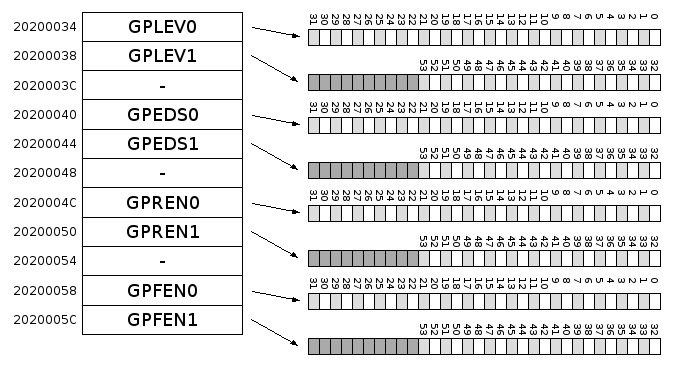
\includegraphics[width=14cm]{graphs/gpio2.png}
  \caption{Otros registros del GPIO 1}
  \label{fig:gpio2}
\end{figure}

\begin{itemize}
  \item {\tt GPLEVn} Estos registros devuelven el valor del pin respectivo. Si dicho pin está
        en torno a 0V devolverá un cero, si está en torno a 3.3V devolverá un 1.
  \item {\tt GPEDSn} Sirven para detectar qué pin ha provocado una interrupción en caso de
        usarlo como lectura. Al escribir en ellos también podemos notificar que ya hemos procesado
        la interrupción y que por tanto estamos listos para que nos vuelvan a interrumpir sobre
        los pines que indiquemos.
  \item {\tt GPRENn} Con estos registros enmascaramos los pines que queremos que provoquen una
        interrupción en flanco de subida, esto es cuando hay una transición de 0 a 1 en el pin
        de entrada.
  \item {\tt GPFENn} Lo mismo que el anterior pero en flanco de bajada.
\end{itemize}

El resto de registros GPIO están en la figura \ref{fig:gpio3}.

\begin{figure}[h]
  \centering
    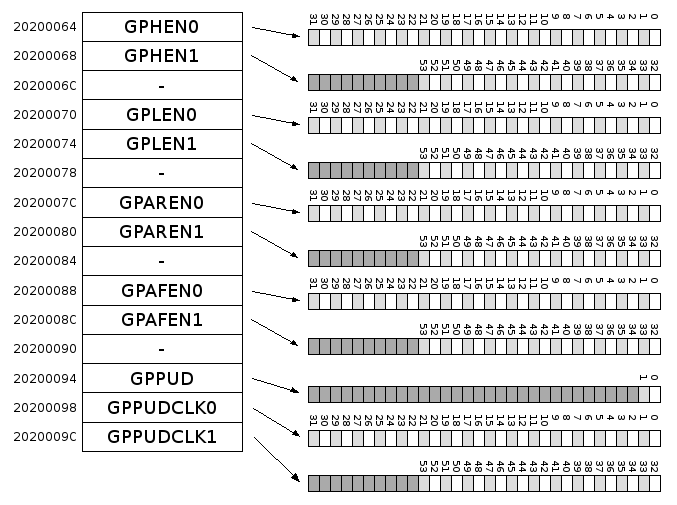
\includegraphics[width=14cm]{graphs/gpio3.png}
  \caption{Otros registros del GPIO 2}
  \label{fig:gpio3}
\end{figure}

\begin{itemize}
  \item {\tt GPHENn} Enmascaramos los pines que provocarán una interrupción al detectar un
        nivel alto (3.3V) por dicho pin.
  \item {\tt GPLENn} Lo mismo que el anterior pero para un nivel bajo (0V).
  \item {\tt GPARENn y GPAFENn} Tienen funciones idénticas a {\tt GPRENn y GPFENn}, pero permiten
        detectar flancos en pulsos de poca duración.
  \item {\tt GPPUD y GPPUDCLKn} Conectan resistencias de pull-up y de pull-down sobre los pines
        que deseemos. Para más información ver el último ejemplo del siguiente capítulo.
\end{itemize}

\subsection{Temporizador del sistema}

Se trata de un reloj que funciona a 1MHz y en cada paso incrementa un contador de 64bits. Nos
viene muy bien para hacer las cuentas porque cada paso del contador se corresponde con un
microsegundo. Los registros asociados al temporizador son los de la figura \ref{fig:systim}.
Básicamente son el contador de 64 bits y cuatro comparadores. El contador está dividido en
dos partes, la parte baja {\tt CLO} y la parte alta {\tt CHI}. La parte alta no nos resulta
interesante, porque tarda poco más de una hora ($2^{32}$ \micro s) en incrementarse y no
va asociado a ningún comparador.

\begin{figure}[h]
  \centering
    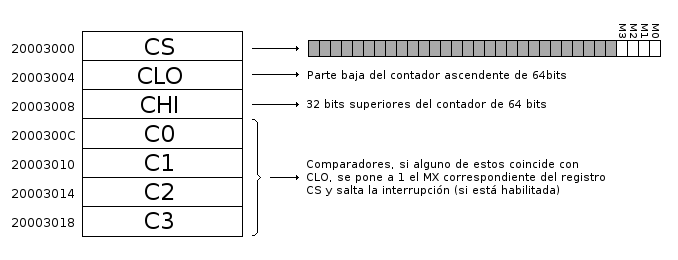
\includegraphics[width=14cm]{graphs/systemtimer.png}
  \caption{System Timer}
  \label{fig:systim}
\end{figure}

Los comparadores son registros que se pueden modificar y se comparan con {\tt CLO}, en el momento
que uno de los 4 comparadores coincida y estén habilitadas las interrupciones para dicho
comparador, se produce una interrupción y se activa el correspondiente bit {\tt Mx}
asociado al registro {\tt CS} (para que en la RTI sepamos qué comparador ha provocado la interrupción).
Los comparadores {\tt C0} y {\tt C2} los emplea la GPU internamente, por lo que nosotros nos
ceñiremos a los comparadores {\tt C1} y {\tt C3}.

Las interrupciones las veremos en la siguiente lección, en los ejemplos de esta sólo vamos
a acceder al registro {\tt CLO} para hacer parpadear al LED a una frecuencia determinada. El
esquema funcional del {\tt System Timer} se muestra en la figura \ref{fig:esqtim}.

\begin{figure}[h]
  \centering
    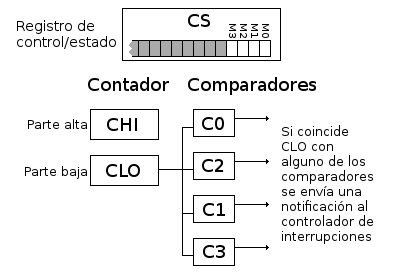
\includegraphics[width=14cm]{graphs/esquematimer.png}
  \caption{Esquema funcional del System Timer}
  \label{fig:esqtim}
\end{figure}


\section{Ejemplos de programas Bare Metal}

\subsection{LED parpadeante con bucle de retardo}

La teoría sobre encender y apagar el LED la sabemos. Lo más sencillo que podemos hacer ahora
es hacer que el LED parpadee continuamente. Vamos a intruducir el siguiente programa en la
Raspberry, antes de probarlo piensa un poco cómo se comportaría el siguiente código.

\begin{lstlisting}[caption={esbn3.s},label={lst:codigoPract4_3}]
        .set    GPBASE,   0x20200000
        .set    GPFSEL0,  0x00
        .set    GPSET0,   0x1c
        .set    GPCLR0,   0x28
.text
        ldr     r0, =GPBASE
/* guia bits           xx999888777666555444333222111000*/
        mov     r1, #0b00001000000000000000000000000000
        str     r1, [r0, #GPFSEL0]
/* guia bits           10987654321098765432109876543210*/
bucle:  mov     r1, #0b00000000000000000000001000000000
        str     r1, [r0, #GPSET0]
        mov     r1, #0b00000000000000000000001000000000
        str     r1, [r0, #GPCLR0]
        b       bucle
\end{lstlisting}

Comprobamos que el LED no parpadea sino que está encendido con menos brillo del normal.
En realidad sí que lo hace, sólo que nuestro ojo es demasiado lento como para percibirlo.
Lo siguiente será ajustar la cadencia del parpadeo a un segundo para que podamos observar
el parpadeo. La secuencia sería apagar el LED, esperar medio segundo, encender el LED,
esperar otro medio segundo y repetir el bucle. Sabemos que el procesador de la Raspberry
corre a 700MHz por lo que vamos a suponer que tarde un ciclo de este reloj en ejecutar
cada instrucción. En base a esto vamos a crear dos bucles de retardo uno tras apagar el LED
y otro tras encenderlo de 500ms cada uno. Un bucle de retardo lo único que hace es esperar
tiempo. 

\begin{lstlisting}[caption={Parte de esbn4.s},label={lst:codigoPract4_4}]
.text
        ldr     r0, =GPBASE
        mov     r1, #0b00001000000000000000000000000000
        str     r1, [r0, #GPFSEL0]
        mov     r1, #0b00000000000000000000001000000000
bucle:  ldr     r2, =7000000
ret1:   subs    r2, #1
        bne     ret1
        str     r1, [r0, #GPSET0]
        ldr     r2, =7000000
ret2:   subs    r2, #1
        bne     ret2
        str     r1, [r0, #GPCLR0]
        b       bucle
\end{lstlisting}

Si lo hacemos con valores teóricos a ciclo por instrucción observaremos como la cadencia del
LED es más lenta de lo esperado, lo que quiere decir que cada iteración del bucle
de retardo tarda más de los dos ciclos que hemos supuesto.
Probamos con cronómetro en mano distintos valores para las constantes hasta comprobar que con
7 millones de iteraciones del bucle se consigue más o menos el medio segundo buscado. Haciendo
cuentas nos salen 50 ciclos por iteracción, bastante más de los 2 ciclos esperados. Esto se
debe a una dependencia de datos (ya que el flag que altera
la orden {\tt subs} es requerido justo después por la instrucción {\tt bne}) y que los saltos
condicionales suelen ser lentos.

\subsection{LED parpadeante con temporizador}

Viendo lo poco preciso que es el temporizar con el bucle de retardo, vamos a sincronizar leyendo
continuamente el valor del {\tt System Timer}.

Como el temporizador va a 1MHz, para temporizar medio segundo lo
único que tenemos que hacer es esperar a que el contador se incremente en medio millón. El código
final quedaría así.

\begin{lstlisting}[caption={esbn5.s},label={lst:codigoPract4_5}]
        .set    GPBASE,   0x20200000
        .set    GPFSEL0,        0x00
        .set    GPSET0,         0x1c
        .set    GPCLR0,         0x28
        .set    STBASE,   0x20003000
        .set    STCLO,          0x04
.text
        ldr     r0, =GPBASE
        mov     r1, #0b00001000000000000000000000000000
        str     r1, [r0, #GPFSEL0]
        mov     r1, #0b00000000000000000000001000000000
        ldr     r2, =STBASE
bucle:  bl      espera
        str     r1, [r0, #GPSET0]
        bl      espera
        str     r1, [r0, #GPCLR0]
        b       bucle

/* rutina que espera medio segundo */
espera: ldr     r3, [r2, #STCLO]
        ldr     r4, =500000
        add     r4, r3
ret1:   ldr     r3, [r2, #STCLO]
        cmp     r3, r4
        bne     ret1
        bx      lr
\end{lstlisting}

\subsection{Sonido con temporizador}

Este ejemplo es exactamente el mismo que el anterior, tan sólo hemos
cambiado el puerto del LED (GPIO 9) al altavoz (GPIO 4) y el tiempo de espera,
para producir un sonido audible.

\begin{lstlisting}[caption={Parte de esbn6.s},label={lst:codigoPract4_6}]
        ldr     r0, =GPBASE
/* guia bits           xx999888777666555444333222111000*/
        mov     r1, #0b00000000000000000001000000000000
        str     r1, [r0, #GPFSEL0]
/* guia bits           10987654321098765432109876543210*/
        mov     r1, #0b00000000000000000000000000010000
        ldr     r2, =STBASE
bucle:  bl      espera
        str     r1, [r0, #GPSET0]
        bl      espera
        str     r1, [r0, #GPCLR0]
        b       bucle

/* rutina que espera 1136 microsegundos */
espera: ldr     r3, [r2, #STCLO]
        ldr     r4, =1136
        add     r4, r3
ret1:   ldr     r3, [r2, #STCLO]
        cmp     r3, r4
        bne     ret1
        bx      lr
\end{lstlisting}

\section{Ejercicios}

\subsection{Cadencia variable con bucle de retardo}

Usando la técnica del bucle de retardo haz que el LED parpadee
cada vez más rápido, hasta que la cadencia sea de 1/4 de segundo.
Una vez llegues a esta cadencia salta de golpe a la cadencia
original de 1 segundo. El tiempo que se tarda en pasar de una
cadencia a otra puede ser el que quieras, siempre que sea
suficiente para poder apreciar el efecto.

\subsection{Cadencia variable con temporizador}

Repite el ejercicio anterior pero empleando el temporizador
interno. Durante los 10 primeros segundos aumentamos la cadencia
del LED desde 1 segundo hasta los 250ms, y en los últimos 10
segundos disminuimos la cadencia al mismo ritmo de tal forma
que el ciclo completo se repite cada 20 segundos.

\chapterend{}


% Capítulo 05.
\chapterbegin{Interrupciones hardware}
\label{chp:Interrupciones}
\minitoc

{\bf Objetivos}: En esta sesión vamos a realizar programas que
utilizan dispositivos de E/S haciendo uso del sistema de
interrupciones hardware. Para poder programar los distintos parámetros
que configuran el entorno de las interrupciones es necesario conocer de
forma detallada cómo funcionan los puertos asociados, ya que
éste es el mecanismo típico mediante el cual el procesador se
comunica con los periféricos.

Hacemos incapié en lo de {\it hardware} porque las
{\it interrupciones software} no son más que las llamadas a sistema
que vimos en el capítulo anterior. Ambas comparten vector de interrupciones,
pero las {\it interrupciones software} son más bien llamadas a subrutinas.

\section{Lectura previa}

El microprocesador se encuentra en un entorno donde existen otros
componentes. La forma de comunicación más usual entre estos
componentes y el microprocesador se denomina interrupción.
Básicamente, una interrupción es una petición que se hace a la CPU
para que detenga temporalmente el trabajo que esté realizando y
ejecute una rutina determinada. 

\subsection{El sistema de interrupciones del ARM}

Decimos que las interrupciones del ARM son {\bf autovectorizadas}.
Cada tipo de interrupción lleva asociado un número (que llamamos
{\bf número de interrupción}, $NI$) que identifica el tipo de servicio a
realizar. En total hay 8 tipos de interrupciones.
A partir de dicho número se calcula la dirección a la que salta la CPU
para atender dicha interrupción. A diferencia de otras arquitecturas
donde los vectores contienen las direcciones de las rutinas de
tratamiento, en ARM no tenemos datos sino instrucciones. Cada vector
contiene normalmente un salto a la rutina de tratamiento correspondiente.
Dicha rutina se suele llamar RTI ({\bf Rutina
de Tratamiento de Interrupción}). En la arquitectura ARMv6
todos los vectores de interrupción se almacenan en una zona de memoria
llamada {\bf tabla de vectores de interrupción}. Esta tabla comienza
en la dirección física 0x00000000 (aunque puede cambiarse por
0xffff0000) y acaba en 0x0000001f y contiene en total 8 vectores de
interrupción. Cuando termina de ejecutarse una RTI,
el procesador continúa ejecutando la instrucción siguiente a la que se
estaba ejecutando cuando se produjo la interrupción.

Existen dos tipos de interrupciones: hardware y software. Las {\bf
interrupciones hardware} son aquellas en las que su activación está
condicionada por el hardware del sistema, ya sea por: 1) {\it
excepciones} provocadas en la ejecución de alguna instrucción o error
grave, o 2) provocadas por la placa base o por cualquier tarjeta
implicada en un canal de E/S.

\noindent La lista del vector de interrupciones es la siguiente.

\begin{longtable}{ p{4.5cm} | p{2.5cm} | p{2cm} | p{4cm}}
\hline
{\bf Excepción} & {\bf Tipo} & {\bf Desplaz.} & {\bf Modo} \\ \hline
Reset                   & Interrupción & {\tt 0x00} & Supervisor \\ \hline
Instrucción no definida & Excepción & {\tt 0x04} & Indefinido \\ \hline
Interrupción software   & Int. software & {\tt 0x08} & Supervisor \\ \hline
Error en prefetch       & Excepción & {\tt 0x0C} & Abort \\ \hline
Error en datos          & Excepción & {\tt 0x10} & Abort \\ \hline
Reservado               & - & {\tt 0x14} & Reservado \\ \hline
IRQ                     & Interrupción & {\tt 0x18} & IRQ \\ \hline
FIQ                     & Interrupción & {\tt 0x1C} & FIQ \\ \hline
\caption{Vector de interrupciones}
\label{tab:excepciones}
\end{longtable}

La última columna se refiere al {\it Modo de operación} que comentamos en el primer
capítulo y que forma parte del registro {\tt cpsr} (ver figura \ref{fig:cpsr}).
Es un estado en el que se encuentra el procesador con una serie de privilegios
con respecto a otros modos y que gracias a ellos podemos construir un sistema operativo
con diferentes capas.

\begin{figure}[h]
  \centering
    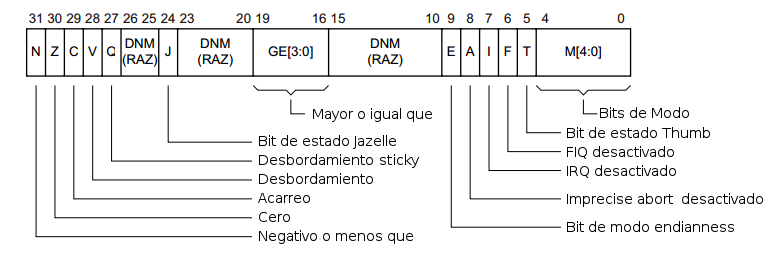
\includegraphics[width=14cm]{graphs/cpsr.png}
  \caption{Registro cpsr}
  \label{fig:cpsr}
\end{figure}

Cada modo tiene sus propios registros {\tt sp}, {\tt lr} y {\tt spsr}
(Saved Program Status Register) de tal
forma que no alteramos la pila ni los flags de la secuencia de programa que interrumpimos. Incluso
el modo {\tt FIQ} tiene 5 registros generales propios (desde {\tt r8} hasta {\tt r12}),
de esta forma si los empleamos en nuestra rutina de tratamiento no tendremos que
salvaguardarlos en pila. En la figura \ref{fig:tablareg} observamos los registros propios
mencionados marcados con un triángulo.

\begin{figure}[h]
  \centering
    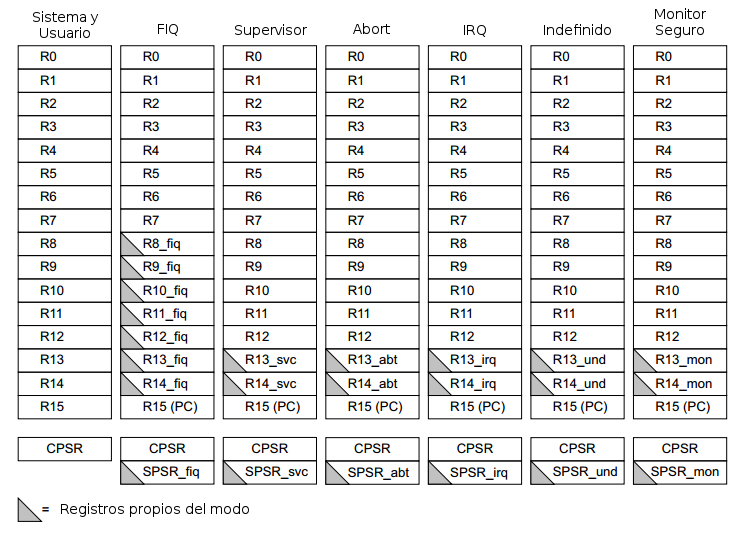
\includegraphics[width=14cm]{graphs/tablaregistros.png}
  \caption{Registros según modo de operación}
  \label{fig:tablareg}
\end{figure}

\begin{itemize}
  \item {\it Reset} es la excepción que permitiría un reset en caliente dentro de la CPU.
Desgraciadamente en la Raspberry no hay forma conocida de forzar esta excepción. Los pines
del conector {\tt P6} en la Raspberry 2.0 y {\tt RUN} en el modelo B+ (ver figura \ref{fig:pinReset})
provocan una secuencia completa de arranque, la que comienza con el bootloader de la GPU y acaba cediendo el control
a la CPU en la dirección 0x8000.

  \item {\it Instrucción no definida} se produce cuando en el flujo de instrucciones nos encontramos
un código de operación que no se corresponde con ninguna instrucción. Normalmente esto se
produce por una corrupción en la memoria de programa o bien que hemos saltado erróneamente
a una zona donde hay datos. También se puede dar el caso de que intentemos ejecutar código
ARM para una plataforma más moderna y nos encontremos con una instrucción no soportada por el
procesador que tenemos.

  \item Las {\it interrupciones software} son subrutinas que se incluyen en el
sistema operativo y que son llamadas desde el programa ejecutando la
instrucción {\tt swi \#n}. No interrumpen realmente nada, pero se
denominan así porque el mecanismo de funcionamiento es el mismo que en
las hardware.

  \item Luego tenemos los errores en {\it prefetch} y {\it datos}. Un error de {\it prefetch} se produce
cuando tratamos de ejecutar una instrucción que momentos antes hemos modificado. Es poco
frecuente y para que se produzca debemos escribir código que sea automodificable, que es
una práctica no deseable y apenas utilizada en dicha arquitectura. Los errores de {\it datos}
son generados normalmente por el manejador de memoria y responden a fallos de alineación, de
traslación, de dominio o de permisos.

  \item Lo siguiente es una entrada reservada, no tiene ninguna funcionalidad ahora
pero es probable que en futuras extensiones sí que la tenga.

  \item Por último están las excepciones que nos interesan y que trataremos en este capítulo, que son
las interrupciones normales {\tt IRQ} y las interrupciones rápidas {\tt FIQ}.
\end{itemize}

Puesto que cada interrupción, $NI$, lleva asociada una rutina, de
alguna forma, debe haber una correspondencia entre este $NI$
y la ubicación del vector asociado, que contiene la instrucción de salto a la rutina que debe
ejecutar cuando se produce la interrupción. La forma de hacerlo es multiplicar por
cuatro el número de interrupción para obtener un desplazamiento
($NI$*4). Se multiplica por 4 porque cada vector de excepción
ocupa 4 bytes (es lo que ocupa una instrucción en ARM).

Cuando se activa una interrupción, la CPU detiene su trabajo para
atenderla. Después, continúa su trabajo donde lo dejó. Los pasos a
seguir para que esto sea posible son:

\begin{enumerate}
  \item Cuando se activa la interrupción, se termina la ejecución de la
    instrucción en curso. A continuación hacemos una copia {\tt cpsr} en el registro
    propio {\tt spsr} correspondiente. De esta forma recordamos los flags de estado
    y el modo que había antes de la interrupción. Una vez hecha la copia se
    procede a cambiar {\tt cpsr}, conmutando al modo correspondiente
    según la tabla \ref{tab:excepciones}.

  \item Seguidamente a lo anterior almacenamos en {\tt lr} (en su registro propio del modo)
    el contenido de {\tt pc+8} (salvo si es un {\tt error en datos} que sería
    {\tt pc+12}). La razón de estos
    desplazamientos es puramente técnica, debido al segmentado de la CPU en
    el momento de hacer la copia el registro {\tt pc} se ha incrementado en 1 ó
    2 instrucciones.

\begin{longtable}{ p{1.8cm} | p{2cm} | p{5cm} }
\hline
{\bf PC} & {\bf Ins.} & {\bf Nombre} \\ \hline
x-4  & i-1 & Instrucción anterior \\ \hline
x & i & Instrucción interrumpida \\ \hline
x+4 & i+1 & Instrucción siguiente \\ \hline
x+8 & i+2 & ...     \\ \hline
x+12 & i+3 & ... \\ \hline
\end{longtable}

    Podemos observarlo gráficamente en la figura \ref{fig:diagramainterrupcion}.

\begin{figure}[h]
  \centering
    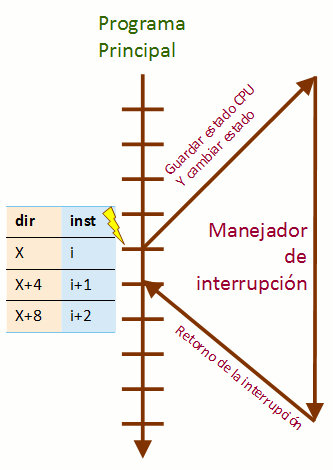
\includegraphics[width=6cm]{graphs/diagramainterrupcion.png}
  \caption{Diagrama de una interrupción}
  \label{fig:diagramainterrupcion}
\end{figure}

  \item Luego saltamos al vector correspondiente ($NI$*4). En esa posición del vector
    encontramos una instrucción de salto a la RTI correspondiente.

  \item Se ejecuta la rutina.

  \item La última instrucción de la rutina es {\tt subs pc, lr, \#4}, que se encarga
    de restaurar los flags originales y el modo copiando {\tt spsr} en {\tt cpsr}.
    Además volvemos al punto donde se interrumpió copiando de {\tt lr} a {\tt pc} (con el
    desplazamiento correspondiente).

   \item Se continúa ejecutando la tarea inicial.
\end{enumerate}

El registro {\tt cpsr} contiene 3 flags globales mediante los cuales podemos habilitar o
inhabilitar las interrupciones: uno para {\tt Abort} llamado {\tt A}, otro para
{\tt IRQ} llamado {\tt I} y el último para {\tt FIQ} denominado {\tt F}.

El manejo de estos flags corre a cuenta del usuario, en ningún momento la CPU enmascara
dichos flags. Por esta razón, si queremos dar prioridad a una interrupción en particular
para no ser interrumpidos nuevamente, debemos enmascarar dichos flags al comienzo de su RTI.

\subsection{Rutina de tratamiento de interrupción}

Es el segmento de código que se ejecuta para atender a una interrupción. Una vez se haya
ejecutado dicha rutina, retomamos la ejecución normal de nuestro programa, justo después de la instrucción
donde lo habíamos interrumpido. Cada rutina de tratamiento debe atender a todas las posibles
fuentes de interrupción de su mismo tipo, con lo que al comienzo de la interrupción se suelen
acceder a los puertos asociados para detectar qué periférico ha causado la interrupción y
actuar en consecuencia.

Si nos interesan {\tt IRQ} y {\tt FIQ}, a lo sumo tendremos que escribir dos
rutinas de tratamiento distintas. Si se produce una {\tt IRQ}, se ejecutará el código
que se encuentre en la dirección {\tt 0x0018}, mientras que si lo que salta es una {\tt IRQ},
la dirección a ejecutar será {\tt 0x001C}. La diferencia entre una {\tt IRQ} y una
{\tt FIQ} es que esta última tiene sus propios registros desde {\tt r8} hasta {\tt r12}
asociados al modo de operación, con lo que podemos prescindir del salvado y recuperación
de estos registros en la RTI, ahorrando un tiempo que en determinadas aplicaciones de
tiempo real puede ser decisivo.

El esqueleto de una RTI es el siguiente.

\begin{lstlisting}
irq_handler:
        push    {lista registros}
        ...
        pop     {lista registros}
        subs    pc, lr, #4
\end{lstlisting}

Vemos que a diferencia de las subrutinas donde salíamos con {\tt lr}, en una RTI salimos
con {\tt lr-4} (si es un {\tt error en datos} sería {\tt lr-8}), a ello se debe que la última
instrucción sea {\tt subs} en lugar de {\tt movs}.
¿Y porqué hay un sufijo {\tt s} al final
de la instrucción {\tt sub}? Pues porque se trata de instrucción especial que sirve para
restaurar el registro {\tt cpsr} que había antes de la interrupción (copia {\tt spsr\_irq} o
{\tt spsr\_fiq} en {\tt cpsr}).

Imaginemos que el programa principal está en modo supervisor y que la interrupción que
esperamos el del tipo IRQ.
Cada modo de operación (en particular el modo IRQ) tiene 3 registros replicados: {\tt sp}, {\tt lr} y {\tt spsr}.
Para evitar confusiones los nombramos con los sufijos de modo {\tt \_svc} y {\tt \_irq} correspondientes.
Cuando ocurre una interrupción pasamos de modo supervisor a modo IRQ, pero antes hemos guardado
el registro {\tt cpsr} en {\tt spsr\_irq}.

Los registros {\tt sp\_svc} y {\tt lr\_svc} no se tocan para nada, con lo que no alteramos ni la
pila ni el registro de retorno del modo supervisor. El registro {\tt lr\_irq} se carga apuntando a la
instrucción {\tt i+2} siguiente a la que fue interrumpida, {\tt pc+8}. El resto de registros debemos salvarlos en pila si tenemos la intención
de modificarlos en nuestra RTI, al tener registro propio {\tt sp\_irq} se trata de una pila
independiente que no interfiere con la principal {\tt sp\_svc}. Luego se ejecuta el código
particular de la RTI, empleando a nuestro antojo los registros previamente salvados, y antes de
acabar la RTI recuperamos con su {\tt pop} correspondiente.

Al terminar la interrupción restauramos {\tt pc} partiendo {\tt lr\_irq} y {\tt cpsr} del registro
{\tt spsr\_irq}. Esto último fuerza un cambio de modo de IRQ a supervisor, conmutando {\tt sp} y {\tt lr}
a sus registros propios {\tt sp\_svc} y {\tt lr\_svc}. Con todo esto conseguimos volver exactamente
al punto del que partíamos minimizando las
operaciones que tiene que hacer la RTI y por tanto el retardo asociado. En otras arquitecturas
además de delegar en la RTI este trabajo, se usa la misma pila de programa, lo que puede
ocasionar problemas si nos importa lo que hay debajo de ésta.

\subsection{Pasos para configurar las interrupciones}

Nosotros vamos a tratar un caso sencillo de programa principal en el cual hacemos las
inicializaciones correspondientes para luego meternos en un bucle infinito y que las
interrupciones hagan su trabajo. Las cosas se pueden complicar metiendo código en
el programa principal concurrente con las interrupciones. Un ejemplo de esto sería
una rutina que dibuja la pantalla en el programa principal, mientras que se aceptan
interrupciones para registrar las pulsaciones del teclado.

Sin embargo nuestro programa principal tras la inicialización será una
instrucción que salta a sí misma continuamente, {\tt bucle: b bucle}.

El orden recomendado es el siguiente, aunque se puede cambiar el mismo salvo el último punto.

\begin{enumerate}
  \item Escribimos en el vector de interrupciones la instrucción de salto necesaria a nuestra RTI.
        Nosotros emplearemos una macro llamada {\tt ADDEXC} que tiene 2 parámetros, vector y
        dirección de la RTI. La macro genera y escribe el código de operación
        del salto, para ver los detalles consultar apéndice \ref{chp:MacroADDEXC}.
        En nuestros ejemplos tendremos IRQs ({\tt 0x18}) y FIQs ({\tt 0x1c}), por
        lo que como mucho haremos dos invocaciones a dicha macro (para dos RTIs distintas).
\begin{lstlisting}
      .macro    ADDEXC  vector, dirRTI
        ldr     r1, =(\dirRTI-\vector+0xa7fffffb)
        ROR     r1, #2
        str     r1, [r0, #\vector]
      .endm
\end{lstlisting}
  \item Inicializamos el puntero de pila (registro {\tt sp}) en todos los modos de operación.
        Al cambiar el modo de operación hay que tener cuidado de no modificar la máscara
        global de interrupciones, ya que comparten el mismo byte bajo de {\tt cpsr}. Como
        sabemos que al comienzo estaban deshabilitadas, las mantenemos igual (bits {\tt I}
        y {\tt F} a 1.
        Los punteros tienen que alojar la pila en zonas distintas donde sepamos que no
        habrá conflictos con la memoria de programa. En los ejemplos en los que usemos FIQ e
        IRQ inicializamos la pila de FIQ
        a {\tt 0x4000}, la de IRQ a {\tt 0x8000} y la del modo Supervisor a {\tt 0x8000000}.
        Como la memoria de programa empieza en {\tt 0x8000} y la pila crece hacia abajo,
        tendremos 16K de pila en modo IRQ, otros 16K en modo FIQ y 128Mb a compartir entre
        programa principal y pila de programa. El mapa de memoria sería el indicado en la figura
        \ref{fig:mapamemoria}

\begin{figure}[h]
  \centering
    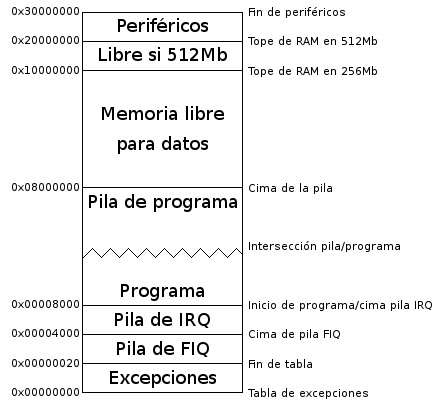
\includegraphics[width=8cm]{graphs/mapamemoria.png}
  \caption{Mapa de memoria en nuestros ejemplos}
  \label{fig:mapamemoria}
\end{figure}

  \item Escribimos código de inicialización ajeno al proceso de interrupción, como por ejemplo
        configurar los GPIOs a salidas donde queramos que actúe un LED.
  \item Ahora viene la inicialización de las interrupciones. Aquí le decimos al sistema qué fuentes
        pueden provocar interrupciones, escribiendo en los puertos asociados. 
  \item El último paso es habilitar las interrupciones globalmente escribiendo en el registro
        {\tt cpsr}. Lo hacemos indirectamente vía otro registro, y la instrucción tiene otro
        nombre pero hace lo mismo que un {\tt mov}. En concreto se llama {\tt msr}, y también hay
        otra equivalente {\tt mrs} si lo que queremos es leer de {\tt cpsr} a un registro.
  \item Después de esto se acaba la inicialización y tendríamos el bucle infinito del que consta
        nuestro programa principal. Si todo ha ido bien las rutinas de tratamiento de interrupción
        se encargarán de hacer funcionar nuestro programa como queramos.
\end{enumerate}

\subsection{El controlador de interrupciones}

Los puertos que componen el controlador de interrupciones son los siguientes.

\begin{figure}[h]
  \centering
    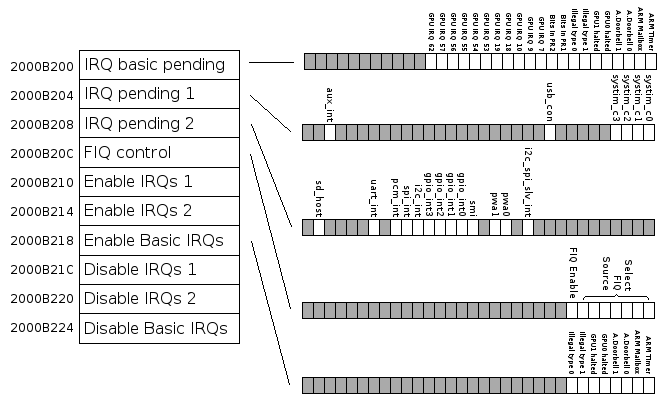
\includegraphics[width=14cm]{graphs/interrupciones.png}
  \caption{Interrupciones}
  \label{fig:interrupciones}
\end{figure}

Las {\tt FIQs} sólo tienen un puerto de control asociado, quedando todo el detalle
en las {\tt IRQs}. Hay tres grupos de tres
puertos cada uno. El primer grupo (Pending) sirve para indicar que hay una interrupción
pendiente, el segundo (Enable) es para habilitar las interrupciones y el tercero (Disable)
para deshabilitarlas. Dentro de cada grupo tenemos un puerto básico que tiene un resumen
sobre el mapa de interrupciones y otros dos puertos que
indican con más detalle la fuente de la interrupción. En el puerto básico
hay fuentes individuales {\tt GPU IRQ x} y bits que engloban a varias fuentes {\tt Bits in PR1},
que por ejemplo indica que el origen hay que buscarlo en el puerto 1. En el puerto 1 están
las primeras 32 posiciones del mapa de interrupciones, mientras que en el puerto 2 están
las 32 últimas.

La documentación oficial sobre el mapa de interrupciones está incompleta, pero buscando un poco
por internet se puede encontrar que las interrupciones asociadas al {\tt System Timer} se
controlan con los 4 primeros bits de la tabla (uno para cada comparador).

En la figura \ref{fig:interrupcionesgrupos} vemos los puertos ordenados en grupos.

\begin{figure}[h]
  \centering
    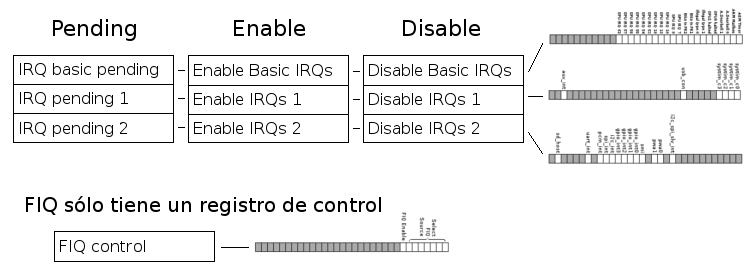
\includegraphics[width=15cm]{graphs/interrupcionesgrupos.png}
  \caption{Agrupación de puertos de interrupciones}
  \label{fig:interrupcionesgrupos}
\end{figure}

La forma habitual de trabajar es usar el puerto apropiado del grupo {\tt Enable} para
habilitar la fuente de interrupción que queramos que nos interrumpa. Luego en el caso de
ser interrumpidos podemos detectar cuál ha sido la fuente leyendo el mismo bit del
grupo {\tt Pending} y finalmente, si pasamos a otra sección del programa donde no queremos
que nos interrumpa más dicha fuente la desactivamos con el grupo {\tt Disable}.

A parte del controlador de interrupciones, cada dispositivo tiene su propio mecanismo de
habilitar/deshabilitar y detectar/notificar la fuente de interrupción. En el caso del GPIO tenemos
los puertos {\tt GPRENn}, {\tt GPFENn}, {\tt GPHENn}, {\tt GPLENn}, {\tt GPARENn} y {\tt GPAFENn}
para habilitar/deshabilitar. Para detectar/notificar están los {\tt GPEDSn}.

Para el temporizador tenemos que {\tt STCS} hace las funciones de detección y notificación. No
existen puertos específicos para habilitar/deshabilitar ya que el controlador de
interrupciones permite habilita/deshabilitar cada comparador por separado.

El único puerto que nos falta por ver es {\tt FIQ control ó INTFIQCON} que hemos
mostrado en la figura \ref{fig:interrupciones}. Antes mostraremos la lista de fuentes
de interrupción aplicables a este puerto.

\begin{table}
\centering
\begin{tabular}{ p{2cm} | p{8cm}} \hline
{\bf Índice} & {\bf Fuente} \\ \hline
0-63  & Interrupciones IRQ 1 y 2 (ver figura \ref{fig:interrupciones})  \\ \hline
64    & ARM Timer  \\ \hline
65    & ARM Mailbox \\ \hline
66    & ARM Doorbell 0 \\ \hline
67    & ARM Doorbell 1 \\ \hline
68    & GPU0 detenida \\ \hline
69    & GPU1 detenida \\ \hline
70    & Acceso ilegal de tipo 1 \\ \hline
71    & Acceso ilegal de tipo 2 \\ \hline
\end{tabular}
\end{table}

Son las mismas fuentes que en IRQ pero condensadas en un único puerto. De 0 a 31 coincide
con la tabla {\tt IRQ 1}, de 32 a 63 con {\tt IRQ 2} y de 64 en adelante con {\tt IRQ Basic}.

El puerto {\tt INTFIQCON} se programa con los 8 bits inferiores, indicando en el bit 7 si
queremos habilitar la fuente, y en los bits del 0 al 6 ponemos el índice de la fuente que
se corresponde con la lista. A diferencia de las IRQ, con las FIQ sólo podemos atender a
una fuente de interrupción. 

\subsection{Ejemplo. Encender LED rojo a los 4 segundos}

Se trata de programar el comparador y las interrupciones para que
transcurrido un tiempo determinado se produzca una interrupción, dentro
de la cual se encienda el LED. Es un caso muy sencillo porque sólo
se va a producir una interrupción que viene de una sola fuente, por
lo que en la RTI lo único que haremos es encender el LED.

El diagrama que vamos a usar es el siguiente.

\begin{figure}[h]
  \centering
    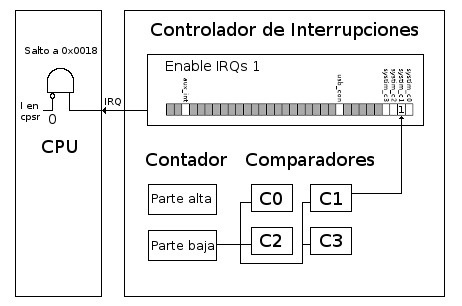
\includegraphics[width=10cm]{graphs/inter1.png}
  \caption{Interrupciones}
  \label{fig:inter1}
\end{figure}

\subsubsection{1. Escribimos en el vector de interrupciones}

  Invocamos la macro para una IRQ, pasándole la etiqueta de nuestra RTI {\tt irq\_handler}.
\begin{lstlisting}
        ADDEXC  0x18, irq_handler
\end{lstlisting}

\subsubsection{2. Inicializamos punteros de pila}

La única forma de acceder a los registros {\tt sp\_irq} y {\tt sp\_fiq} es cambiando de modo
 y modificando el registro {\tt sp} correspondiente.

El modo viene indicado en la parte más baja del registro {\tt cpsr}, el cual modificaremos
con la instrucción especial {\tt msr}. En la figura \ref{fig:cpsr} vemos el contenido completo
del registro {\tt cpsr}. Como {\tt cpsr} es un registro muy heterogéneo, usamos
sufijos para acceder a partes concretas de él. En nuestro caso sólo nos
interesa cambiar el byte bajo del registro, añadimos el sufijo {\tt \_c} llamándolo {\tt cpsr\_c},
para no alterar el resto del registro. Esta parte comprende el modo de operación
y las máscaras globales de las interrupciones. Otra referencia útil es {\tt cpsr\_f} que modifica
únicamente la parte de flags (byte alto). Las otras 3 referencias restantes apenas se usan y
son {\tt cpsr\_s} (Status) para el tercer byte, {\tt cpsr\_x} (eXtended) para el segundo byte y
{\tt cpsr\_csxf} para modificar los 4 bytes a la vez.

En la siguiente tabla vemos cómo se codifica el modo de operación.

\begin{longtable}{ p{1.8cm} | p{2cm} | p{5cm} | p{1cm} | p{1cm} }
\hline
{\bf Hex} & {\bf Binario} & {\bf Modo de operación} \\ \hline
0x10 & 10000 & Usuario        \\ \hline
0x11 & 10001 & FIQ            \\ \hline
0x12 & 10010 & IRQ            \\ \hline
0x13 & 10011 & Supervisor     \\ \hline
0x16 & 10110 & Monitor seguro \\ \hline
0x17 & 10111 & Abort          \\ \hline
0x1B & 11011 & Indefinido     \\ \hline
0x1F & 11111 & Sistema        \\ \hline
\end{longtable}

Como las interrupciones globales de IRQ y FIQ están desactivadas (estado por defecto tras
el reset), mantenemos a 1 dichos bits.

El código que inicializa los punteros de pila es el siguiente:

\begin{lstlisting}
        mov     r0, #0b11010010   @ Modo IRQ, FIQ&IRQ desact
        msr     cpsr_c, r0
        mov     sp, #0x8000
        mov     r0, #0b11010011   @ Modo SVC, FIQ&IRQ desact
        msr     cpsr_c, r0
        mov     sp, #0x8000000
\end{lstlisting}

En concreto a {\tt 0x8000} y {\tt 0x8000000} para los modos {\tt IRQ} y
{\tt Supervisor} respectivamente.

\subsubsection{3. Código de inicialización ajeno a interrupciones}

En el ejemplo que tenemos entre manos se trata de configurar los puertos
GPIO de entrada y de salida, inicializar temporizadores. En casos más complejos tendríamos que
inicializar estructuras de datos, rellenar las tablas que sean precalculadas y en general
cualquier tarea de inicialización requerida para hacer funcionar nuestro programa.

El código para asignar el sentido al pin GPIO 9 es el siguiente:

\begin{lstlisting}
        ldr     r0, =GPBASE
/* guia bits           xx999888777666555444333222111000*/
        mov     r1, #0b00001000000000000000000000000000
        str     r1, [r0, #GPFSEL0]
\end{lstlisting}

Luego programamos el comparador para que salte la interrupción a los 4,19 segundos:

\begin{lstlisting}
        ldr     r0, =STBASE
        ldr     r1, [r0, #STCLO]
        add     r1, #0x400000     @4,19 segundos
        str     r1, [r0, #STC1]
\end{lstlisting}

\subsubsection{4. Inicializamos interrupciones localmente}

Consiste en escribir en los puertos asociados dependiendo de las fuentes que querramos
activar. En este primer ejemplo habilitamos el comparador
{\tt C1} del temporizador como fuente de interrupción:

\begin{lstlisting}
        ldr     r0, =INTBASE
        mov     r1, #0b0010
        str     r1, [r0, #INTENIRQ1]
\end{lstlisting}

\subsubsection{5. Habilitamos interrupciones globalmente}

Se trata de poner a cero el bit correspondiente en {\tt cpsr}. El siguiente código habilita
interrupciones del tipo IRQ:

\begin{lstlisting}
        mov     r0, #0b01010011   @ Modo SVC, IRQ activo
        msr     cpsr_c, r0
\end{lstlisting}

\subsubsection{6. Resto del programa principal}

Como hemos adelantado, en todos nuestros ejemplos será un bucle infinito:

\begin{lstlisting}
bucle:  b       bucle
\end{lstlisting}

A continuación mostramos el listado del ejemplo completo:

\begin{lstlisting}[caption={inter1.s},label={lst:codigoPract5_1}]
        .include  "inter.inc"
.text
/* Agrego vector interrupción */
        ADDEXC  0x18, irq_handler

/* Inicializo la pila en modos IRQ y SVC */
        mov     r0, #0b11010010   @ Modo IRQ, FIQ&IRQ desact
        msr     cpsr_c, r0
        mov     sp, #0x8000
        mov     r0, #0b11010011   @ Modo SVC, FIQ&IRQ desact
        msr     cpsr_c, r0
        mov     sp, #0x8000000

/* Configuro GPIO 9 como salida */
        ldr     r0, =GPBASE
/* guia bits           xx999888777666555444333222111000*/
        mov     r1, #0b00001000000000000000000000000000
        str     r1, [r0, #GPFSEL0]

/* Programo contador C1 para futura interrupción */
        ldr     r0, =STBASE
        ldr     r1, [r0, #STCLO]
        add     r1, #0x400000     @4,19 segundos
        str     r1, [r0, #STC1]

/* Habilito interrupciones, local y globalmente */
        ldr     r0, =INTBASE
        mov     r1, #0b0010
        str     r1, [r0, #INTENIRQ1]
        mov     r0, #0b01010011   @ Modo SVC, IRQ activo
        msr     cpsr_c, r0

/* Repetir para siempre */
bucle:  b       bucle

/* Rutina de tratamiento de interrupción */
irq_handler:
        push    {r0, r1}          @ Salvo registros

        ldr     r0, =GPBASE
/* guia bits           10987654321098765432109876543210*/
        mov     r1, #0b00000000000000000000001000000000
        str     r1, [r0, #GPSET0] @ Enciendo LED

        pop     {r0, r1}          @ Recupero registros
        subs    pc, lr, #4        @ Salgo de la RTI
\end{lstlisting}

Observamos que la RTI es muy sencilla, aparte del esqueleto tenemos tres instrucciones
encargadas de encender el LED en cuestión.

\subsection{Ejemplos de aplicación}

Vamos a crear un archivo {\tt inter.inc} donde guardaremos las constantes
asociadas a los puertos y también la macro {\tt ADDEXC}, esta última
se explica en detalle en el apéndice \ref{chp:MacroADDEXC}. De esta forma evitamos escribir
siempre las mismas constantes, haciendo el código más sencillo de mantener.

\begin{lstlisting}[caption={inter.inc},label={lst:codigoPract5_0}]
      .macro    ADDEXC  vector, dirRTI
        ldr     r1, =(\dirRTI-\vector+0xa7fffffb)
        ROR     r1, #2
        str     r1, [r0, #\vector]
      .endm
        .set    GPBASE,   0x20200000
        .set    GPFSEL0,        0x00
        .set    GPFSEL1,        0x04
        .set    GPFSEL2,        0x08
        .set    GPSET0,         0x1c
        .set    GPCLR0,         0x28
        .set    GPEDS0,         0x40
        .set    GPREN0,         0x58
        .set    GPPUD,          0x94
        .set    GPPUDCLK0,      0x98
        .set    STBASE,   0x20003000
        .set    STCS,           0x00
        .set    STCLO,          0x04
        .set    STC1,           0x10
        .set    STC3,           0x18
        .set    INTBASE,  0x2000b000
        .set    INTFIQCON,     0x20c
        .set    INTENIRQ1,     0x210
        .set    INTENIRQ2,     0x214
\end{lstlisting}

El método para incluir el código fuente de un fichero dentro de otro es mediante
la macro {\tt .include}, todos nuestros ficheros comienzarán con lo siguiente.

\begin{lstlisting}
        .include  "inter.inc"
\end{lstlisting}

\subsection{Parpadeo de todos los LEDs}

Sería hacer lo mismo que en la lección anterior pero empleando interrupciones y aplicando
la salida simultáneamente a los 6 LEDs en lugar de sólo al primero. La novedad en lo
que a interrupciones se refiere consiste en reprogramar el comparador C1 cada vez que
se produzca una interrupción, de esta forma conseguimos interrupciones periódicas en lugar
de una única interrupción.

Veamos el código:

\begin{lstlisting}[caption={inter2.s},label={lst:codigoPract5_2}]
        .include  "inter.inc"
.text
/* Agrego vector interrupción */
        ADDEXC  0x18, irq_handler

/* Inicializo la pila en modos IRQ y SVC */
        mov     r0, #0b11010010   @ Modo IRQ, FIQ&IRQ desact
        msr     cpsr_c, r0
        mov     sp, #0x8000
        mov     r0, #0b11010011   @ Modo SVC, FIQ&IRQ desact
        msr     cpsr_c, r0
        mov     sp, #0x8000000

/* Configuro GPIOs 9, 10, 11, 17, 22 y 27 como salida */
        ldr     r0, =GPBASE
        mov     r1, #0b00001000000000000000000000000000
        str     r1, [r0, #GPFSEL0]
/* guia bits           xx999888777666555444333222111000*/
        ldr     r1, =0b00000000001000000000000000001001
        str     r1, [r0, #GPFSEL1]
        ldr     r1, =0b00000000001000000000000001000000
        str     r1, [r0, #GPFSEL2]

/* Programo contador C1 para dentro de 2 microsegundos */
        ldr     r0, =STBASE
        ldr     r1, [r0, #STCLO]
        add     r1, #2
        str     r1, [r0, #STC1]

/* Habilito interrupciones, local y globalmente */
        ldr     r0, =INTBASE
        mov     r1, #0b0010
        str     r1, [r0, #INTENIRQ1]
        mov     r0, #0b01010011   @ Modo SVC, IRQ activo
        msr     cpsr_c, r0

/* Repetir para siempre */
bucle:  b       bucle

/* Rutina de tratamiento de interrupción */
irq_handler:
        push    {r0, r1, r2}

/* Conmuto variable de estado del LED */
        ldr     r0, =ledst    @ Leo puntero a v. ledst
        ldr     r1, [r0]      @ Leo variable
        eors    r1, #1        @ Invierto bit 0, act. flag Z
        str     r1, [r0]      @ Escribo variable

/* Enciendo o apago todos los LEDs en función del flag Z */
        ldr     r0, =GPBASE
/* guia bits           10987654321098765432109876543210*/
        ldr     r1, =0b00001000010000100000111000000000
        streq   r1, [r0, #GPSET0]
        strne   r1, [r0, #GPCLR0]

/* Reseteo estado interrupción de C1 */
        ldr     r0, =STBASE
        mov     r1, #0b0010
        str     r1, [r0, #STCS]

/* Programo siguiente interrupción medio segundo después */
        ldr     r1, [r0, #STCLO]
        ldr     r2, =500000       @1 Hz
        add     r1, r2
        str     r1, [r0, #STC1]

/* Recupero registros y salgo */
        pop     {r0, r1, r2}
        subs    pc, lr, #4

/* Ubicación de la variable ledst */
ledst:  .word   0
\end{lstlisting}

Y vamos enumerando, por orden, los pasos que hemos seguido. En primer lugar apuntamos a nuestra
RTI en el vector de interrupciones:

\begin{lstlisting}
        ADDEXC  0x18, irq_handler
\end{lstlisting}

Luego inicializamos los punteros de pila:

\begin{lstlisting}
        mov     r0, #0b11010010   @ Modo IRQ, FIQ&IRQ desact
        msr     cpsr_c, r0
        mov     sp, #0x8000
        mov     r0, #0b11010011   @ Modo SVC, FIQ&IRQ desact
        msr     cpsr_c, r0
        mov     sp, #0x8000000
\end{lstlisting}

Lo siguiente es configurar los pines GPIO asociados a los 6 LEDs como salidas:

\begin{lstlisting}
        ldr     r0, =GPBASE
        mov     r1, #0b00001000000000000000000000000000
        str     r1, [r0, #GPFSEL0]
/* guia bits           xx999888777666555444333222111000*/
        ldr     r1, =0b00000000001000000000000000001001
        str     r1, [r0, #GPFSEL1]
        ldr     r1, =0b00000000001000000000000001000000
        str     r1, [r0, #GPFSEL2]
\end{lstlisting}

Preparamos el comparador {\tt C1} para que al cabo de dos microsegundos nos proporcione la primera
interrupción:

\begin{lstlisting}
        ldr     r0, =STBASE
        ldr     r1, [r0, #STCLO]
        add     r1, #2
        str     r1, [r0, #STC1]
\end{lstlisting}

Para después habilitar las interrupciones asociadas al comparador {\tt C1}:

\begin{lstlisting}
        ldr     r0, =INTBASE
        mov     r1, #0b0010
        str     r1, [r0, #INTENIRQ1]
\end{lstlisting}

Y finalmente habilitar las interrupciones {\tt IRQ} globalmente, entrando luego en
el bucle infinito:

\begin{lstlisting}
        mov     r0, #0b01010011   @modo SVC, IRQ activo
        msr     cpsr_c, r0
bucle:  b       bucle
\end{lstlisting}

Ya hemos terminado con el programa principal, que como veremos más adelante va a ser
siempre muy parecido.

Lo interesante está en la RTI, que es donde hacemos parpadear los LEDs y configuramos
el comparador para la siguiente interrupción.

El estado de los LEDs (si están apagados o encendidos) lo guardamos en la variable
{\tt ledst}, que conmutamos entre cero y uno mediante un {\tt OR} exclusivo. Al
actualizar los {\tt flags} tras esta operación, tenemos que si el resultado fue
cero nos lo indica el {\tt flag Z} activo, mientras que estará inactivo en el
caso contrario (resultado 1). Mediante las instrucciones de ejecución condicional
{\tt streq} y {\tt strne} enviamos la orden al puerto que enciende los LEDs o al
puerto que los apaga, respectivamente:

\begin{lstlisting}
irq_handler:
        push    {r0, r1, r2}

        ldr     r0, =ledst    @ Leo puntero a v. ledst
        ldr     r1, [r0]      @ Leo variable
        eors    r1, #1        @ Invierto bit 0, act. flag Z
        str     r1, [r0]      @ Escribo variable

        ldr     r0, =GPBASE
/* guia bits           10987654321098765432109876543210*/
        ldr     r1, =0b00001000010000100000111000000000
        streq   r1, [r0, #GPSET0]
        strne   r1, [r0, #GPCLR0]
\end{lstlisting}

Luego escribimos un 1 en el {\tt M1} de {\tt CS}, para resetear el estado de coincidencia, ya
que de lo contrario el gestor de interrupciones verá el bit siempre a 1 y no lanzará más
interrupciones. Resulta confuso tener que escribir un 1 en el puerto para almacenar un 0, pero
de un modo similar a lo que ocurre con el puerto {\tt GPCLR0} del GPIO es para ahorrar
operaciones y que la RTI sea más rápida. Así no hay que leer el puerto, aplicar una máscara y
volver a escribir en el mismo puerto, con una escritura es suficiente:

\begin{lstlisting}
        ldr     r0, =STBASE
        mov     r1, #0b0010
        str     r1, [r0, #STCS]
\end{lstlisting}

Luego tenemos que actualizar el puerto comparador, de lo contrario tardará poco más
de una hora en cambiar de estado el LED (es lo que tarda el contador en dar una vuelta
completa). Para ello leemos el contador ({\tt CLO}) y le añadimos 500000 al valor leído. Como cada
cuenta equivale a un microsegundo, este añadido al contador supone medio segundo, lo
que nos da la cadencia de un segundo que buscamos. El resultado de la suma lo escribimos
en el comparador ({\tt C1}):

\begin{lstlisting}
        ldr     r1, [r0, #STCLO]
        ldr     r2, =500000       @1 Hz
        add     r1, r2
        str     r1, [r0, #STC1]
\end{lstlisting}

Por último restauramos los registros utilizados y salimos de la RTI. Más abajo tenemos la
definición de la variable {\tt ledst}, como no tenemos sección de datos aparte la ponemos
al final del código:

\begin{lstlisting}
        pop     {r0, r1, r2}
        subs    pc, lr, #4

ledst:  .word   0
\end{lstlisting}

\subsection{Control de LEDs rojos con pulsadores}

En este ejemplo cambiamos de fuente de interrupción, en lugar del temporizador empleamos
los pulsadores. Queremos que al pulsar un botón se encienda el LED rojo del mismo lado del
pulsador, dejando el otro apagado.

El esquema sería el de la figura \ref{fig:inter3}.

\begin{figure}[h]
  \centering
    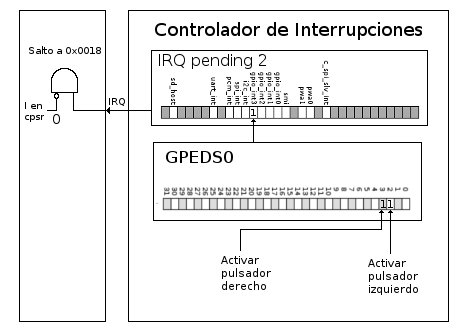
\includegraphics[width=14cm]{graphs/inter3.png}
  \caption{Interrupciones}
  \label{fig:inter3}
\end{figure}

Y el código fuente lo vemos a continuación:

\begin{lstlisting}[caption={inter3.s},label={lst:codigoPract5_3}]
        .include  "inter.inc"
.text
/* Agrego vector interrupción */
        ADDEXC  0x18, irq_handler

/* Inicializo la pila en modos IRQ y SVC */
        mov     r0, #0b11010010   @ Modo IRQ, FIQ&IRQ desact
        msr     cpsr_c, r0
        mov     sp, #0x8000
        mov     r0, #0b11010011   @ Modo SVC, FIQ&IRQ desact
        msr     cpsr_c, r0
        mov     sp, #0x8000000

/* Configuro GPIOs 9 y 10 como salida */
        ldr     r0, =GPBASE
        mov     r1, #0b00001000000000000000000000000000
        str     r1, [r0, #GPFSEL0]
/* guia bits           xx999888777666555444333222111000*/
        mov     r1, #0b00000000000000000000000000000001
        str     r1, [r0, #GPFSEL1]

/* Enciendo LEDs       10987654321098765432109876543210*/
        mov     r1, #0b00000000000000000000011000000000
        str     r1, [r0, #GPSET0]

/* Habilito pines GPIO 2 y 3 (botones) para interrupciones*/
        mov     r1, #0b00000000000000000000000000001100
        str     r1, [r0, #GPREN0]
        ldr     r0, =INTBASE

/* Habilito interrupciones, local y globalmente */
        mov     r1, #0b00000000000100000000000000000000
/* guia bits           10987654321098765432109876543210*/
        str     r1, [r0, #INTENIRQ2]
        mov     r0, #0b01010011   @ Modo SVC, IRQ activo
        msr     cpsr_c, r0

/* Repetir para siempre */
bucle:  b       bucle

/* Rutina de tratamiento de interrupción */
irq_handler:
        push    {r0, r1}
        ldr     r0, =GPBASE
/* Apago los dos LEDs rojos  54321098765432109876543210*/
        mov     r1, #0b00000000000000000000011000000000
        str     r1, [r0, #GPCLR0]
/* Consulto si se ha pulsado el botón GPIO2 */
        ldr     r1, [r0, #GPEDS0]
        ands    r1, #0b00000000000000000000000000000100
/* Sí: Activo GPIO 9; No: Activo GPIO 10 */
        movne   r1, #0b00000000000000000000001000000000
        moveq   r1, #0b00000000000000000000010000000000
        str     r1, [r0, #GPSET0]
/* Desactivo los dos flags GPIO pendientes de atención
   guia bits                 54321098765432109876543210*/
        mov     r1, #0b00000000000000000000000000001100
        str     r1, [r0, #GPEDS0]
        pop     {r0, r1}
        subs    pc, lr, #4
\end{lstlisting}

Obviamos los dos primeros pasos (apuntar a RTI e inicialización de punteros de pila) puesto
que son idénticos al ejemplo anterior.

Lo siguiente que tenemos es configurar e inicializar los puertos del GPIO. Por un lado
ponemos los correspondientes a los LEDs rojos (GPIO 9 y GPIO 10) como salida. Por otro
lado escribimos un uno en ambos LEDs, para que al arrancar veamos los dos LEDs encendidos.
Así sabemos que el programa está cargado a la espera de que activemos los pulsadores:

\begin{lstlisting}
        ldr     r0, =GPBASE
        ldr     r1, =0b00001000000000000000000000000000
        str     r1, [r0, #GPFSEL0]
/* guia bits           xx999888777666555444333222111000*/
        ldr     r1, =0b00000000000000000000000000000001
        str     r1, [r0, #GPFSEL1]
/* guia bits           10987654321098765432109876543210*/
        mov     r1, #0b00000000000000000000011000000000
        str     r1, [r0, #GPSET0]
\end{lstlisting}

Luego habilitamos las interrupciones particulares del GPIO en el puerto
{\tt GPREN0}, en concreto las que entran por los pulsadores (GPIO 2 y GPIO 3). 
Para que las peticiones se propaguen desde el GPIO al controlador de interrupciones
habilitamos el bit 20 del puerto {\tt INTENIRQ2}:

\begin{lstlisting}
        mov     r1, #0b00000000000000000000000000001100
        str     r1, [r0, #GPREN0]
        ldr     r0, =INTBASE
/* guia bits           10987654321098765432109876543210*/
        mov     r1, #0b00000000000100000000000000000000
        str     r1, [r0, #INTENIRQ2]
\end{lstlisting}

Para terminar activando globalmente las IRQ y metiéndonos en el bucle infinito:

\begin{lstlisting}
        mov     r0, #0b01010011   @ Modo SVC, IRQ activo
        msr     cpsr_c, r0
bucle:  b       bucle
\end{lstlisting}

Veamos ahora el aspecto que tiene la RTI. Lo primero es poner los LEDs susceptibles de
encenderse (los LEDs rojos) a cero:

\begin{lstlisting}
irq_handler:
        push    {r0, r1}
        ldr     r0, =GPBASE
/* Apaga los dos LEDs rojos  54321098765432109876543210*/
        mov     r1, #0b00000000000000000000011000000000
        str     r1, [r0, #GPCLR0]
\end{lstlisting}

Testeamos cuál de los dos pulsadores se ha activado, indicándolo en el flag Z:

\begin{lstlisting}
/* Consulto si se ha pulsado el botón GPIO2 */
        ldr     r1, [r0, #GPEDS0]
        ands    r1, #0b00000000000000000000000000000100
\end{lstlisting}

En función del flag Z encendemos uno u otro LED:

\begin{lstlisting}
/* Sí: Activo GPIO 9; No: Activo GPIO 10 */
        movne   r1, #0b00000000000000000000001000000000
        moveq   r1, #0b00000000000000000000010000000000
        str     r1, [r0, #GPSET0]
\end{lstlisting}

Y finalmente desactivamos los dos flags GPIO pendientes de atención:

\begin{lstlisting}
        mov     r1, #0b00000000000000000000000000001100
        str     r1, [r0, #GPEDS0]
        pop     {r0, r1}
        subs    pc, lr, #4
\end{lstlisting}

\subsection{Parpadeo secuencial de LEDs con sonido por altavoz}

En este ejemplo vamos a trabajar con el temporizador, pero esta vez vamos a complicar
un poco las cosas. En lugar de una fuente vamos a atender simultáneamente las peticiones
de los comparadores {\tt C1} y {\tt C3}.

\begin{figure}[h]
  \centering
    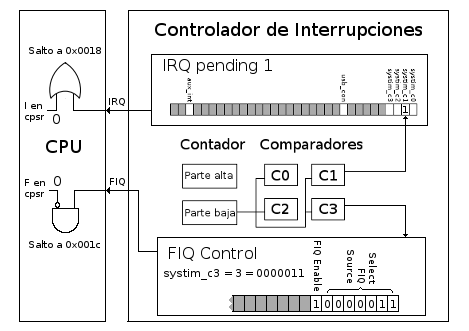
\includegraphics[width=14cm]{graphs/inter4.png}
  \caption{Interrupciones}
  \label{fig:inter4}
\end{figure}

Con esta segunda fuente vamos a controlar el altavoz, como podemos
observar en la figura \ref{fig:inter3}. Sacar un tono
puro por el altavoz es equivalente a hacer parpadear un LED, lo único que cambia es que usamos
otro pin distinto {\tt GPIO 4} y aumentamos la frecuencia para que sea audible (a 1 Hz el oído
humano no captaría sonido alguno). Utilizaremos la frecuencia estándar de afinación
de 440 Hz, que coincide con el tono de espera de marcado en telefonía fija.

Por otro lado en lugar de hacer parpadear todos los LEDs lo que haremos es repetir una
secuencia de 6 posiciones en la que en todo momento sólo uno de los 6 LEDs está encendido, que
va cambiando de izquierda a derecha (aparentando movimiento) y cuando se llegue al sexto LED
comenzamos de nuevo desde el primero. Para dar más sensación de movimiento disminuimos el periodo
a 200 milisegundos.

La clave de todo está en saber cuál de los dos comparadores ha producido la interrupción (se
puede dar el caso en que salten los dos a la vez). Ésto se puede hacer de dos formas distintas:
o bien leemos el bit asociado {\tt systim\_cx} en el puerto {\tt IRQ pending 1}, o bien leemos
el {\tt Mx} del puerto {\tt CS}. Elegimos el segundo caso, así no gastamos otro puerto más
para almacenar {\tt INTBASE}.

El código completo del ejemplo es el siguiente:

\begin{lstlisting}[caption={inter4.s},label={lst:codigoPract5_4},escapeinside={(*@}{@*)}]
        .include  "inter.inc"
.text
/* Agrego vector interrupción */
        ADDEXC  0x18, irq_handler

/* Inicializo la pila en modos IRQ y SVC */
        mov     r0, #0b11010010   @ Modo IRQ, FIQ&IRQ desact
        msr     cpsr_c, r0
        mov     sp, #0x8000
        mov     r0, #0b11010011   @ Modo SVC, FIQ&IRQ desact
        msr     cpsr_c, r0
        mov     sp, #0x8000000

/* Configuro GPIOs 4, 9, 10, 11, 17, 22 y 27 como salida */
        ldr     r0, =GPBASE
        ldr     r1, =0b00001000000000000001000000000000
        str     r1, [r0, #GPFSEL0]
/* guia bits           xx999888777666555444333222111000*/
        ldr     r1, =0b00000000001000000000000000001001
        str     r1, [r0, #GPFSEL1]
        ldr     r1, =0b00000000001000000000000001000000
        str     r1, [r0, #GPFSEL2]

/* Programo C1 y C3 para dentro de 2 microsegundos */
        ldr     r0, =STBASE
        ldr     r1, [r0, #STCLO]
        add     r1, #2
        str     r1, [r0, #STC1]
        str     r1, [r0, #STC3]

/* Habilito interrupciones, local y globalmente */
        ldr     r0, =INTBASE
        mov     r1, #0b1010
        str     r1, [r0, #INTENIRQ1]
        mov     r0, #0b01010011   @ Modo SVC, IRQ activo
        msr     cpsr_c, r0

/* Repetir para siempre */
bucle:  b       bucle

/* Rutina de tratamiento de interrupción */
irq_handler:
        push    {r0, r1, r2, r3}

/* Leo origen de la interrupción */
        ldr     r0, =STBASE
        ldr     r1, =GPBASE
        ldr     r2, [r0, #STCS]
        ands    r2, #0b0010
        beq     sonido

/* Si es C1, ejecuto secuencia de LEDs */
        ldr     r2, =cuenta
/* guia bits           10987654321098765432109876543210*/
        ldr     r3, =0b00001000010000100000111000000000
        str     r3, [r1, #GPCLR0] @ Apago todos los LEDs
        ldr     r3, [r2]          @ Leo variable cuenta
        subs    r3, #1            @ Decremento
        moveq   r3, #6            @ Si es 0, volver a 6
        str     r3, [r2]          @ Escribo cuenta
        ldr     r3, [r2, +r3, LSL #2] @ Leo secuencia
        str     r3, [r1, #GPSET0] @ Escribo secuencia en LEDs

/* Reseteo estado interrupción de C1 */
        mov     r3, #0b0010
        str     r3, [r0, #STCS]

/* Programo siguiente interrupción en 200ms */
        ldr     r3, [r0, #STCLO]
        ldr     r2, =200000       @ 5 Hz
        add     r3, r2
        str     r3, [r0, #STC1]

/* (*@\color[rgb]{0,0.5,0}{¿}@*)Hay interrupción pendiente en C3? */
        ldr     r3, [r0, #STCS]
        ands    r3, #0b0100
        beq     final             @ Si no, salgo

/* Si es C3, hago sonar altavoz
sonido: ldr     r2, =bitson
        ldr     r3, [r2]
        eors    r3, #1            @ Invierto estado
        str     r3, [r2]
        mov     r3, #0b10000      @ GPIO 4 (altavoz)
        streq   r3, [r1, #GPSET0] @ Escribo en altavoz
        strne   r3, [r1, #GPCLR0] @ Escribo en altavoz

/* Reseteo estado interrupción de C3 */
        mov     r3, #0b1000
        str     r3, [r0, #STCS]

/* Programo interrupción para sonido de 440 Hz */
        ldr     r3, [r0, #STCLO]
        ldr     r2, =1136         @ Contador para 440 Hz
        add     r3, r2
        str     r3, [r0, #STC3]

/* Recupero registros y salgo */
final:  pop     {r0, r1, r2, r3}
        subs    pc, lr, #4

bitson: .word   0             @ Bit 0 = Estado del altavoz
cuenta: .word   1             @ Entre 1 y 6, LED a encender
/* guia bits      7654321098765432109876543210*/
secuen: .word   0b1000000000000000000000000000
        .word   0b0000010000000000000000000000
        .word   0b0000000000100000000000000000
        .word   0b0000000000000000100000000000
        .word   0b0000000000000000010000000000
        .word   0b0000000000000000001000000000
\end{lstlisting}

Como es muy parecido al ejemplo de antes, sólo vamos a comentar las diferencias que encontremos.
La primera de ellas es que además de los 6 GPIOs de los LEDs, configuramos como salida un séptimo
pin, el GPIO 4, para manejar el altavoz:

\begin{lstlisting}
        ldr     r0, =GPBASE
        ldr     r1, =0b00001000000000000001000000000000
        str     r1, [r0, #GPFSEL0]
\end{lstlisting}

El siguiente código es para incluir el comparador {\tt C3} (además del {\tt C1} que había
anteriormente), tanto para proporcionar la primera
interrupción como para habilitarla individualmente:

\begin{lstlisting}
        ldr     r0, =STBASE
        ldr     r1, [r0, #STCLO]
        add     r1, #2
        str     r1, [r0, #STC1]
        str     r1, [r0, #STC3]
        ldr     r0, =INTBASE
        mov     r1, #0b1010
        str     r1, [r0, #INTENIRQ1]
\end{lstlisting}

Ya hemos acabado con el programa principal, veamos ahora la RTI. Primero mostramos la estructura
del código y luego las rutinas individuales tanto para el manejo de LEDs como para el
altavoz:

\begin{lstlisting}
irq_handler:
        push    {r0, r1, r2, r3}
        ldr     r0, =STBASE
        ldr     r1, =GPBASE
        ldr     r2, [r0, #STCS]
        ands    r2, #0b0010
        beq     sonido

        [ manejo de LEDs ]

        ldr     r3, [r0, #STCS]
        ands    r3, #0b0100
        beq     final
sonido:
        [ manejo de altavoz ]

final:  pop     {r0, r1, r2, r3}
        subs    pc, lr, #4
\end{lstlisting}

Los registros {\tt r0} y {\tt r1} los hacemos apuntar a la base del {\tt System Timer} y del
{\tt GPIO} y no tocamos dichos valores durante toda la interrupción, vamos a estar
constantemente leyendo y escribiendo puertos y resulta incómodo tener que cargar la
base cada vez.

Es un error muy habitual suponer que la fuente de la interrupción sólo ha sido una, aunque
la gran mayoría de las veces sea así se puede dar el caso de que coincidan los dos comparadores
a la vez. De la misma forma si sabemos que sólo hay dos fuentes y una de ellas no ha
provocado la interrupción, por descarte ha tenido que ser la otra, podemos ahorrarnos la
comprobación.

El flujo sería el siguiente: leemos {\tt M1} para ver si la interrupción la ha provocado el
comparador de {\tt C1}, si ha sido así ejecutamos el código de manejo de LEDs; si no,
saltamos directamente al manejo del altavoz (sabemos seguro que la fuente viene de ahí).

Tras el código del manejo de LEDs leemos {\tt M3} para saber si además de {\tt C1} ha
saltado también el comparador {\tt C3}. Si no ha saltado, lo más normal, salimos por
{\tt final}; si lo ha hecho, procesamos la interrupción con el código de manejo del altavoz
para luego salir de la RTI.

Estos programas no son fáciles de crear y nunca funcionan a la primera. Es una buena práctica
hacer funcionar por separado el código de los LEDs y el código del altavoz, y una vez
comprobemos que funcionan, aglutinarlo en una única RTI. De esta forma aislamos lo máximo
posible los errores que podamos cometer, es muy fácil equivocarse en una tontería y estar
dándole vueltas al código sin encontrar el fallo. A diferencia de los primeros capítulos
que disponíamos de {\tt gdb}, en Bare Metal no tenemos acceso a ningún depurador.

Prosigamos ahora con el código de manejo de LEDs. Recordemos que hemos complicado un poco
las cosas para emitir una secuencia en lugar de un simple parpadeo. Para ello mostramos
el código seguido de las variables empleadas en el mismo:

\begin{lstlisting}
        ldr     r2, =cuenta
/* guia bits           10987654321098765432109876543210*/
        ldr     r3, =0b00001000010000100000111000000000
        str     r3, [r1, #GPCLR0] @ Apago todos los LEDs
        ldr     r3, [r2]          @ Leo variable cuenta
        subs    r3, #1            @ Decremento
        moveq   r3, #6            @ Si es 0, volver a 6
        str     r3, [r2]          @ Escribo cuenta
        ldr     r3, [r2, +r3, LSL #2] @ Leo secuencia#2]
        str     r3, [r1, #GPSET0] @ Escribo secuencia en LEDs
        mov     r3, #0b0010
        str     r3, [r0, #STCS]
        ldr     r3, [r0, #STCLO]
        ldr     r2, =200000       @ 5 Hz
        add     r3, r2
        str     r3, [r0, #STC1]
        [...]
cuenta: .word   1             @ Entre 1 y 6, LED a encender
/* guia bits      7654321098765432109876543210*/
secuen: .word   0b1000000000000000000000000000
        .word   0b0000010000000000000000000000
        .word   0b0000000000100000000000000000
        .word   0b0000000000000000100000000000
        .word   0b0000000000000000010000000000
        .word   0b0000000000000000001000000000
\end{lstlisting}

En la variable {\tt cuenta} almacenamos un contador que va desde 6 hasta 1, que actua
como índice para el array {\tt secuen}. Al decrementar aprovechamos la propia instrucción de
resta para comprobar que se ha llegado al final de la cuenta (0), y en dicho caso
restablecemos la cuenta a 6 mediante la instrucción de ejecución condicional {\tt moveq}.

En el array secuen tenemos almacenadas las posiciones que corresponden a los LEDs dentro del
puerto {\tt GPSET0}, cada posición del array es para encender un LED en concreto. Antes
de esto hemos apagado todos los LEDs enviando el valor que codifica todos los LEDs al
puerto {\tt GPCLR0}.

A parte de sacar la secuencia correspondiente debemos especificar cuándo será la siguiente
interrupción. Como hicimos en el ejemplo anterior, esto se resuelve leyendo el valor del
puerto {\tt STCLO}, sumándole 200000 (200 milisegundos) y escribiéndolo en el comparador
{\tt STC1}.

Acabado el código de manejo de LEDs, ya sólo falta por explicar el manejo del altavoz:

\begin{lstlisting}
sonido: ldr     r2, =bitson
        ldr     r3, [r2]
        eors    r3, #1            @ Invierto estado
        str     r3, [r2]
        mov     r3, #0b10000      @ GPIO 4 (altavoz)
        streq   r3, [r1, #GPSET0] @ Escribo en altavoz
        strne   r3, [r1, #GPCLR0] @ Escribo en altavoz
        mov     r3, #0b1000
        str     r3, [r0, #STCS]
        ldr     r3, [r0, #STCLO]
        ldr     r2, =1136         @ Contador para 440 Hz
        add     r3, r2
        str     r3, [r0, #STC3]
        [...]
bitson: .word   0
\end{lstlisting}

Es un calco de la rutina que hacía parpadear todos los LEDs, cambiando
el valor que se envia a {\tt GPCLR0/GPSET0}, el comparador que es {\tt C3} en lugar de {\tt C1},
y el valor que sumamos al temporizador, que se corresponde a 440 Hz en vez de a 1 Hz.

\subsection{Manejo de FIQs y sonidos distintos para cada LED}

Este ejemplo es muy parecido al anterior pero con cambios sutiles. El hecho de cambiar una de
las dos IRQs por una FIQ incluso simplifica el código, ya que tienen distintas RTIs y en cada
una la fuente de interrupción es única, por lo que no hay que comprobar nada ni hacer saltos.

\begin{figure}[h]
  \centering
    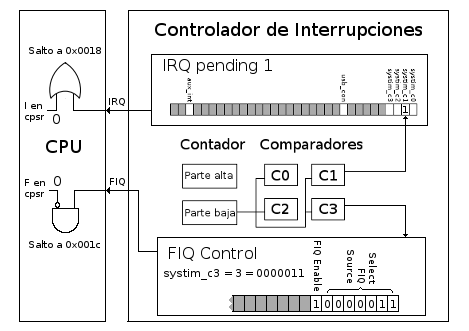
\includegraphics[width=14cm]{graphs/inter5.png}
  \caption{Interrupciones}
  \label{fig:inter5}
\end{figure}

Empecemos con el programa principal. Aquí sí que hay cambios porque tenemos que agregar un
elemento nuevo al vector de interrupciones, inicializar el puntero de pila del modo FIQ y activar
la fuente de interrupción FIQ local y globalmente:

\begin{lstlisting}[caption={Programa principal de inter5.s},label={lst:codigoPract5_5}]
/* Agrego vectores de interrupción */
        ADDEXC  0x18, irq_handler
        ADDEXC  0x1c, fiq_handler

/* Inicializo la pila en modos FIQ, IRQ y SVC */
        mov     r0, #0b11010001   @ Modo FIQ, FIQ&IRQ desact
        msr     cpsr_c, r0
        mov     sp, #0x4000
        mov     r0, #0b11010010   @ Modo IRQ, FIQ&IRQ desact
        msr     cpsr_c, r0
        mov     sp, #0x8000
        mov     r0, #0b11010011   @ Modo SVC, FIQ&IRQ desact
        msr     cpsr_c, r0
        mov     sp, #0x8000000

/* Configuro GPIOs 4, 9, 10, 11, 17, 22 y 27 como salida */
        ldr     r0, =GPBASE
        ldr     r1, =0b00001000000000000001000000000000
        str     r1, [r0, #GPFSEL0]
/* guia bits           xx999888777666555444333222111000*/
        ldr     r1, =0b00000000001000000000000000001001
        str     r1, [r0, #GPFSEL1]
        ldr     r1, =0b00000000001000000000000001000000
        str     r1, [r0, #GPFSEL2]

/* Programo C1 y C3 para dentro de 2 microsegundos */
        ldr     r0, =STBASE
        ldr     r1, [r0, #STCLO]
        add     r1, #2
        str     r1, [r0, #STC1]
        str     r1, [r0, #STC3]

/* Habilito C1 para IRQ */
        ldr     r0, =INTBASE
        mov     r1, #0b0010
        str     r1, [r0, #INTENIRQ1]

/* Habilito C3 para FIQ */
        mov     r1, #0b10000011
        str     r1, [r0, #INTFIQCON]

/* Habilito interrupciones globalmente */
        mov     r0, #0b00010011   @ Modo SVC, FIQ&IRQ activo
        msr     cpsr_c, r0

/* Repetir para siempre */
bucle:  b       bucle
\end{lstlisting}

Queremos que FIQ se active con {\tt C3}, que es el bit 3 del {\tt IRQ 1}, por tanto
índice 3 para la fuente {\tt FIQ}. Como veis, la única pega que tienen las FIQs es que
sólo admiten una fuente de interrupción. Además del índice ponemos el bit 7 a uno para
indicar que queremos habilitar dicha fuente, siendo la constante {\tt 0b10000011}.

Ahora veamos el manejador IRQ (la RTI) que, como hemos adelantado, es más sencilla que en el
ejemplo anterior:

\begin{lstlisting}
/* Rutina de tratamiento de interrupción IRQ */
irq_handler:
        push    {r0, r1, r2}
        ldr     r0, =GPBASE
        ldr     r1, =cuenta

/* Apago todos LEDs    10987654321098765432109876543210*/
        ldr     r2, =0b00001000010000100000111000000000
        str     r2, [r0, #GPCLR0]

        ldr     r2, [r1]          @ Leo variable cuenta
        subs    r2, #1            @ Decremento
        moveq   r2, #6            @ Si es 0, volver a 6
        str     r2, [r1], #-4     @ Escribo cuenta
        ldr     r2, [r1, +r2, LSL #3] @ Leo secuencia
        str     r2, [r0, #GPSET0] @ Escribo secuencia en LEDs

/* Reseteo estado interrupción de C1 */
        ldr     r0, =STBASE
        mov     r2, #0b0010
        str     r2, [r0, #STCS]

/* Programo siguiente interrupción en 500ms */
        ldr     r2, [r0, #STCLO]
        ldr     r1, =500000       @ 2 Hz
        add     r2, r1
        str     r2, [r0, #STC1]

/* Recupero registros y salgo */
        pop     {r0, r1, r2}
        subs    pc, lr, #4
\end{lstlisting}

Observamos que al acceder a la tabla {\tt secuen} multiplicamos el índice por 8 en lugar de
por 4. Esto es así porque hemos incluído en dicha tabla el valor de la longitud de onda (inverso
de la frecuencia) con la que queremos que suene cada LED, la zona de datos es ésta:

\begin{lstlisting}
bitson: .word   0             @ Bit 0 = Estado del altavoz
cuenta: .word   1             @ Entre 1 y 6, LED a encender
secuen: .word   0b1000000000000000000000000000
        .word   716           @ Retardo para nota 6
        .word   0b0000010000000000000000000000
        .word   758           @ Retardo para nota 5
/* guia bits      7654321098765432109876543210*/
        .word   0b0000000000100000000000000000
        .word   851           @ Retardo para nota 4
        .word   0b0000000000000000100000000000
        .word   956           @ Retardo para nota 3
/* guia bits      7654321098765432109876543210*/
        .word   0b0000000000000000010000000000
        .word   1012          @ Retardo para nota 2
        .word   0b0000000000000000001000000000
        .word   1136          @ Retardo para nota 1
\end{lstlisting}

Serían las notas puras que van después del LA estándar de 440 Hz (1136), cuyos semitonos se
obtienen multiplicando la frecuencia por raíz duodécima de 2, que es aproximadamente 1,05946.
Las notas serían, en hercios: LA (440), SI (493,88), DO (523,25), RE (587,33), MI (659,26) y
FA (698,46).

Finalmente tenemos el manejador de FIQ asociado al altavoz. La elección de la fuente de
interrupción no es arbitraria, hemos escogido FIQ para el altavoz porque se ejecutará más veces
que el cambio de LEDs, concretamente 220 veces más con la nota más grave. En estos ejemplos
no importa, pero en casos reales donde el tiempo de CPU es un recurso limitado, los ciclos
que nos ahorramos con una FIQ en un proceso crítico pueden ser determinantes:

\begin{lstlisting}
/* Rutina de tratamiento de interrupción FIQ */
fiq_handler:
        ldr     r8, =GPBASE
        ldr     r9, =bitson

/* Hago sonar altavoz invirtiendo estado de bitson */
        ldr     r10, [r9]
        eors    r10, #1
        str     r10, [r9], #4

/* Leo cuenta y luego elemento correspondiente en secuen */
        ldr     r10, [r9]
        ldr     r9, [r9, +r10, LSL #3]

/* Pongo estado altavoz según variable bitson */
        mov     r10, #0b10000     @ GPIO 4 (altavoz)
        streq   r10, [r8, #GPSET0]
        strne   r10, [r8, #GPCLR0]

/* Reseteo estado interrupción de C3 */
        ldr     r8, =STBASE
        mov     r10, #0b1000
        str     r10, [r8, #STCS]

/* Programo retardo según valor leído en array */
        ldr     r10, [r8, #STCLO]
        add     r10, r9
        str     r10, [r8, #STC3]

/* Salgo de la RTI */
        subs    pc, lr, #4
\end{lstlisting}

El código sería idéntico al de una IRQ si no fuera porque empleamos registros a partir de
{\tt r8} en lugar de a partir de {\tt r0}, y no los salvaguardamos con las instrucciones
{\tt push/pop}. La razón es que el modo de operación FIQ es el único que tiene sus propios
registros {\tt r8-r12} (ver figura \ref{fig:tablareg}) con el objetivo de no perder el tiempo
guardando y recuperando datos de la pila. En situaciones más críticas podemos incluso ubicar
la RTI justo al final del vector de interrupciones. Esta tabla no contiene datos, sino instrucciones,
y lo que hace la CPU cuando ocurre una excepción es saltar (ejecutar) a la dirección asociada en
dicho vector. Así que cada elemento es una instrucción de salto que apunta a su RTI
correspondiente, de no ser un salto se solaparía con el siguiente elemento del vector. Excepto
el último elemento del vector, que no se solaparía con nada y que corresponde a las
interrupciones FIQ. Se ha escogido intencionalmente así para ahorrarse el salto inicial.

\subsection{Control de luces/sonido con pulsadores en lugar temporizadores}

Los pulsadores izquierdo y derecho de nuestra placa externa están asociados a los
puertos {\tt GPIO 2} y {\tt GPIO 3} respectivamente. Veremos
cómo se genera una interrupción al pulsar cualquiera de los mismos.

\begin{figure}[h]
  \centering
    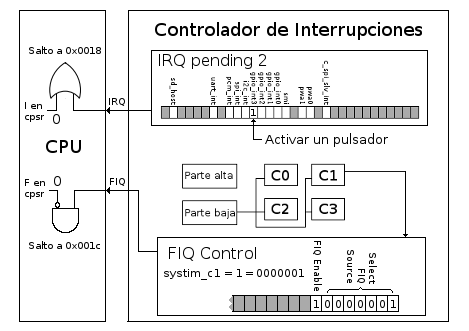
\includegraphics[width=14cm]{graphs/inter6.png}
  \caption{Interrupciones}
  \label{fig:inter6}
\end{figure}

El programa principal sería el siguiente:

\begin{lstlisting}[caption={Programa principal de inter6.s},label={lst:codigoPract5_6}]
/* Agrego vectores de interrupción */
        ADDEXC  0x18, irq_handler
        ADDEXC  0x1c, fiq_handler

/* Inicializo la pila en modos FIQ, IRQ y SVC */
        mov     r0, #0b11010001   @ Modo FIQ, FIQ&IRQ desact
        msr     cpsr_c, r0
        mov     sp, #0x4000
        mov     r0, #0b11010010   @ Modo IRQ, FIQ&IRQ desact
        msr     cpsr_c, r0
        mov     sp, #0x8000
        mov     r0, #0b11010011   @ Modo SVC, FIQ&IRQ desact
        msr     cpsr_c, r0
        mov     sp, #0x8000000

/* Configuro GPIOs 4, 9, 10, 11, 17, 22 y 27 como salida */
        ldr     r0, =GPBASE
        ldr     r1, =0b00001000000000000001000000000000
        str     r1, [r0, #GPFSEL0]
/* guia bits           xx999888777666555444333222111000*/
        ldr     r1, =0b00000000001000000000000000001001
        str     r1, [r0, #GPFSEL1]
        ldr     r1, =0b00000000001000000000000001000000
        str     r1, [r0, #GPFSEL2]

/* Enciendo LEDs       10987654321098765432109876543210*/
        mov     r1, #0b00000000000000000000001000000000
        str     r1, [r0, #GPSET0]

/* Habilito pines GPIO 2 y 3 (botones) para interrupciones*/
        mov     r1, #0b00000000000000000000000000001100
        str     r1, [r0, #GPREN0]

/* Programo C1 para dentro de 2 microsegundos */
        ldr     r0, =STBASE
        ldr     r1, [r0, #STCLO]
        add     r1, #2
        str     r1, [r0, #STC1]

/* Habilito GPIO para IRQ */
        ldr     r0, =INTBASE
/* guia bits           10987654321098765432109876543210*/
        mov     r1, #0b00000000000100000000000000000000
        str     r1, [r0, #INTENIRQ2]

/* Habilito C1 para FIQ */
        mov     r1, #0b10000001
        str     r1, [r0, #INTFIQCON]

/* Habilito interrupciones globalmente */
        mov     r0, #0b00010011   @modo SVC, FIQ&IRQ activo
        msr     cpsr_c, r0

/* Repetir para siempre */
bucle:  b       bucle
\end{lstlisting}

Lo nuevo que vemos aquí es una escritura en el puerto {\tt GPREN0}. De esta forma
le decimos al controlador de interrupciones que esos pines del GPIO serán los únicos que
provoquen interrupciones, concretamente flancos con de subida síncronos (justo
en el momento en que el botón toca fondo).

El manejador FIQ es idéntico al del ejemplo anterior, saca el sonido que corresponde al LED
por el altavoz, cambiando {\tt C3} por {\tt C1}.

Lo más relevante de este ejemplo está en la RTI asociada a la IRQ, que es la siguiente:

\begin{lstlisting}
irq_handler:
        push    {r0, r1, r2}
        ldr     r0, =GPBASE
        ldr     r1, =cuenta

/* Apago todos LEDs    10987654321098765432109876543210*/
        ldr     r2, =0b00001000010000100000111000000000
        str     r2, [r0, #GPCLR0]

/* Leo botón pulsado */
        ldr     r2, [r0, #GPEDS0]
        ands    r2, #0b00000000000000000000000000001000
        beq     incre

/* Si es botón izquierdo, decrementar */
        str     r2, [r0, #GPEDS0] @ Reseteo flag b. izq
        ldr     r2, [r1]          @ Leo variable cuenta
        subs    r2, #1            @ Decremento
        moveq   r2, #6            @ Si es 0, volver a 6
        b       conti             @ Salto a conti

/* Si es botón derecho, incrementar */
incre:  mov     r2, #0b00000000000000000000000000000100
        str     r2, [r0, #GPEDS0] @ Reseteo flag b. der
        ldr     r2, [r1]          @ Leo variable cuenta
        add     r2, #1            @ Incremento
        cmp     r2, #7            @ Comparo si llego a 7
        moveq   r2, #1            @ Si es 7, volver a 1

/* Actualizo variable, enciendo LED y salgo */
conti:  str     r2, [r1], #-4     @ Escribo variable cuenta
        ldr     r2, [r1, +r2, LSL #3] @ Leo secuencia
        str     r2, [r0, #GPSET0] @ Escribo secuencia en LEDs
        pop     {r0, r1, r2}      @ Recupero registros
        subs    pc, lr, #4        @ Salgo RTI
\end{lstlisting}

Tenemos una bifurcación (saltos condicionales) debido a que cada botón es una fuente distinta
de interrupción y tenemos que distinguir qué botón se ha pulsado. Aquí por suerte tenemos
un puerto totalmente análogo al {\tt STCS} de los temporizadores. Se llama {\tt GPEDS0}
(también hay otro {\tt GPEDS1} para los GPIOs de 32 a 53 que no necesitamos) y sirve tanto
para saber qué fuente ha producido la interrupción como para resetear su estado (y así permitir
volver a ser interrumpidos por el mismo pin GPIO).

Con la instrucción {\tt ands} comprobamos si un determinado bit está a 1 y lo indicamos en el
flag Z. También podría valer la instrucción {\tt tst}, que tiene la ventaja de no destruir
el registro a la salida (de la misma forma que {\tt cmp} es el equivalente no destructivo de
{\tt subs}).

Y por último debemos sacar la secuencia inversa a la que teníamos para que al pulsar el
botón izquierdo las luces vayan hacia la izquierda y que con el botón derecho vayan en el otro
sentido. Si la secuencia de izquierda a derecha era  (6, 5, 4, 3, 2, 1, 6, 5, 4...), la
inversa sería (1, 2, 3, 4, 5, 6, 1...). Es decir, incrementamos y cuando llegamos a 7
lo convertimos en 1. Ésto se hace con el siguiente fragmento:

\begin{lstlisting}
        add     r2, #1            @ Incremento
        cmp     r2, #7            @ Comparo si llego a 7
        moveq   r2, #1            @ Si es 7, volver a 1
\end{lstlisting}

Nótese que aquí la opción destructiva {\tt subs} (en lugar de {\tt cmp}) no nos vale porque
necesitamos el valor del registro después. Sí que podemos cambiarlo por un {\tt teq} (la
alternativa no destructiva de {\tt eors}).

\section{Ejercicios}

\subsection{Todo con IRQs}

Modifica el último ejemplo ({\tt inter5.s}) para controlar el altavoz también con IRQs,
prescindiendo totalmente de las interrupciones FIQs.

\subsection{Alargar secuencia a 10 y parpadeo}

Partiendo de {\tt inter5.s} (o del resultado del ejercicio anterior) haz las siguientes
modificaciones. Si te resulta más cómodo, realízalas por orden.

\begin{itemize}
  \item Sacar de la secuencia el LED 6 (el de más a la derecha) y ponerlo a parpadear
        continuamente con una cadencia de un segundo. En este momento tendrás que acortar
        la secuencia a 5.
  \item Duplica la secuencia a 10. Para ello utiliza el código Morse aplicado a los dígitos
        (todos tienen longitud 5). Cambia el punto (tono corto) por LED apagado y el guión
        (tono largo) por LED encendido. Por supuesto los nuevos códigos tendrán su sonido
        asociado, sigue las notas (saltándote sostenidos y bemoles) para completar la tabla.
\end{itemize}

\subsection{Tope de secuencia y limitar sonido}

Partiendo de {\tt inter5.s} (o del resultado del ejercicio anterior) haz las siguientes
modificaciones. Si te resulta más cómodo, realízalas por orden.

\begin{itemize}
  \item Hasta ahora si llegamos al límite de la secuencia hemos comenzado por el principio,
        haciendo que la secuencia sea circular tanto en un sentido como en otro. Pues bien,
        ahora tienes que detectar dichos límites (tanto superior como inferior), poniendo
        una especie de tope al llegar al límite, que impida avanzar más. En caso de intentar
        avanzar en el sentido prohibido al llegar a un tope, en lugar de sacar el sonido que
        corresponda por el altavoz, auméntalo una escala (tope superior) o disminúyelo también
        una escala (tope inferior).
  \item Como habrás observado el sonido continuo resulta un tanto molesto después de un tiempo.
        Y con la indicación de los LEDs tenemos información suficiente para saber en qué
        posición de la secuencia estamos. Altera el programa para que sólamente suene el altavoz
        mientras el botón está pulsado, o lo que es lo mismo, para el sonido del altavoz cuando
        detectes un flanco de bajada en la señal GPIO correspondiente.
\end{itemize}

\subsection{Reproductor de melodía sencilla}

Escoge una melodía sencilla y trata de interpretarla. Emplea los LEDs a tu gusto para que
cambien según la nota que esté sonando. Implementa las siguientes funciones en los pulsadores.

\begin{itemize}
  \item \textbf{Pulsador izquierdo.} Cambio de tempo. La melodía debe comenzar a tempo normal (llamémoslo 1),
        y variar desde tempo lento (0) y tempo rápido (2) según la secuencia (0, 1, 2, 0...) cada
        vez que pulsemos dicho botón.
  \item \textbf{Pulsador derecho.} Iniciar/Parar/Reanudar. La melodía tiene una duración determinada y
        cuando acaba deja de sonar, no suena en modo bucle todo el tiempo. Si pulsamos dicho botón
        cuando está en silencio después que haya sonado la melodía, la función correspondiente
        sería la de iniciarla. Si lo pulsamos durante la reproducción actuaría a modo de pause
        (los LEDs se quedan congelados en el estado en el que estén), parando y reanudando la
        reproducción de la música.
\end{itemize}

En este ejemplo puedes profundizar todo lo que quieras. Por ejemplo empieza codificando los
silencios, éstos son muy importantes y también forman parte de la melodía. Un segundo paso sería
codificar la duración de las notas, si no lo has hecho ya. También es posible tener varios
instrumentos sonando a la vez, aunque sólo dispongamos de un altavoz, busca por internet {\tt
1-bit music} o {\tt beeper music} si quieres saber cómo se hace.

\chapterend{}


\part{Parte tercera.}
\chapterbeginx{Conclusiones y líneas futuras}

Tras haber estudiado detenidamente las prácticas diseñadas en
torno a la arquitectura x86 hicimos una comparativa entre
arquitecturas. A pesar de ser las enormes diferencias que separan
ARM de x86 hemos tratado de seguir el mismo guión argumental
de las prácticas.

Al comienzo de cada lección suele haber una serie de conceptos
teóricos, esta parte apenas se ha tocado con ligeras modificaciones
para mantener la coherencia con la nueva arquitectura. El problema
viene una vez avanzamos en la lección, ya que la forma de actuar
es completamente distinta. En x86 básicamente tenemos todo el
hardware a nuestra disposición, podemos comunicarnos a muy bajo
nivel mediante puertos E/S, a bajo nivel mediante interrupciones
software a la BIOS, o a medio/bajo haciendo lo mismo bajo MS-DOS.

En ARM está todo más jerarquizado. Desde Linux no podemos
comunicarnos directamente con el hardware, el más bajo nivel al
que aspiramos es con interrupciones software bajo kernel. También
tenemos acceso a librerías, sin embargo estas se hacen con un
mecanismo distinto, mediante llamadas a funciones empleando la
convención AAPCS.

Aunque no sea exactamente igual, hemos creado una equivalencia entre
la BIOS del PC y el kernel de Linux, entre las ISR (Interrupt Service
Routines) del MS-DOS y las llamadas a funciones de librerías externas,
y finalmente hemos recurrido al Bare Metal para mostrar cómo se
accede directamente al hardware.

Hemos estudiado a fondo la plataforma Raspberry Pi, sobre todo lo
referente al subsistema E/S y el acceso en Bare Metal. Hemos
buscado dispositivos que sean simples pero que a la vez abarquen
todos los aspectos requeridos desde un punto de vista didáctico,
sobre todo que puedan ser accedidos tanto mediante polling como
vía interrupciones.

Llegamos a la conclusión de que con el puerto GPIO y el System Timer
se cubrían todos los aspectos, centrando las prácticas Bare Metal
en torno a estos. Vimos la necesidad de diseñar una placa de extensión
para aumentar la funcionalidad de la Raspberry Pi, y de esta forma
ilustrar mejor los ejemplos en Bare Metal. Gracias a los pulsadores,
el buzzer y los LEDs el alumno puede ir experimentando con el código
y aprendiendo los distintos mecanismos que hay para manejarlos.

En la adaptación de las prácticas es donde más cambios hemos
realizado, debido a la diferencia entre arquitecturas y a que una
conversión más literal de las mismas habría resultado un tanto
forzada. Hemos tratado de seguir un orden más natural, por ejemplo
al introducir los LEDs. Primero tratamos de simplemente encender
un LED, luego nos centramos en hacerlo parpadear, y a medida que
las prácticas avanzan hacemos cosas más complicadas como una
secuencia animada que involucre a varios LEDs.

En cuanto al subsistema gráfico hemos experimentado con él, pero al
final hemos decidido excluirlo para las prácticas debido a la
dificultad logística y económica que supone dotar a los laboratorios
de monitores con entrada HDMI ó Video Compuesto. Los que hay sólo
tienen VGA, y aunque hay aparatos conversores, haría falta también
un sistema de conmutación práctico ya que se requiere trabajar a la vez
con el PC y la Raspberry.

Hemos simplificado al máximo el conexionado y el proceso de carga de
programas Bare Metal. En lugar de conectarnos a la Raspberry por el
típico puerto Ethernet para trabajar con Linux, hemos aprovechado el
puerto serie (necesario para Bare Metal) para hacer la misma función,
con lo que nos ahorramos un cable Ethernet y un slot libre en el switch o
router. El único elemento necesario para trabajar con la Raspberry
(aparte de la placa de expansión) es un conversor USB-Serie que cuesta
en torno a un euro. Este dispositivo tendría 3 funciones: sirve para
alimentar la Raspberry, para trabajar con ella en Linux a modo de terminal
y para cargar (también depurar) programas en Bare Metal.

Especial atención hemos puesto en la carga Bare Metal. Aunque en teoría
se puedan ejecutar programas Bare Metal simplemente reemplazando el
archivo kernel.img de la tarjeta SD, a la hora de desarrollar este
mecanismo resulta tedioso. Extraer la tarjeta, meterla en un PC,
reemplazar el archivo, extraerla del PC, introducirla en la Raspberry
y resetear la misma es una tarea que requiere su tiempo. Aunque un minuto
no suponga mucho tiempo si lo haces una sola vez, a medida que vas
probando modificación tras otra, el proceso se vuelve repetitivo y
aburrido. Hemos optimizado el ciclo de desarrollo mediante un bootloader
en la tarjeta SD que lee del puerto serie y ejecuta el programa Bare
Metal que se le envíe. También hemos pedido conversores USB-Serie
especiales que disponen de un pin de más, que empleamos
para forzar el reset de la Raspberry, que de otra forma habría que
desenchufar y enchufar (o a lo sumo pulsar un botón).

De esta forma la carga de programas Bare Metal se vuelve muy ágil, y
en cuestión de 1 ó 2 segundos podemos tener cargado un nuevo programa
desde la última modificación que hagamos.

Hemos tratado de aproximar al alumno a esta plataforma de
la forma más natural posible, empleando la cadena de herramientas GNU
para ensamblado, compilado, enlazado y depuración, que además de ser
gratuita está bastante extendida en la comunidad (e incluida en la
propia distribución). También hemos escogido Raspbian como distribución
de Linux porque es con diferencia la más popular. Está basada en Debian,
por lo que resulta apropiada para usuarios con poca experiencia en Linux.

Nuestra intención es que el alumno además de aprender disfrute de la
asignatura. Con esta plataforma es posible porque si el alumno lo desea
puede adquirir una Raspberry por su propia cuenta y complementar las
prácticas desde casa. Por esta razón hemos dotado al
laboratorio con el doble de placas de expansión que Raspberries. Así
podrán ser prestadas al alumno que las solicite, ya sea para continuar
el trabajo que se ha quedado pendiente en el laboratorio o para
experimentar con sus propios desarrollos.

Como líneas futuras está el ya mencionado subsistema gráfico. También puede
resultar interesante explotar las posibilidades que brinda el coprocesador
matemático (ó VFP) u otros dispositivos más complejos como el teclado,
el audio o el acceso a la tarjeta SD.

Otra línea no explorada puede ser la depuración en Bare Metal, si bien hemos
probado un sistema que permite depurar por el puerto serie, hemos decidido
no incluirlo para no sobrecargar al alumno. Tampoco es realmente necesaria,
los ejemplos Bare Metal son más bien sencillos y el alumno puede repasar
el código para tratar de encontrar dónde falla.

En este proyecto hemos tratado de buscar un acercamiento sencillo y didáctico
para aprender ensamblador y familiarizarse con la plataforma. Pero nada impide
hacer cosas más complejas dando por aprendidos estos conocimientos en
asignaturas posteriores. Un ejemplo puede ser para Sistemas Operativos. Saber
combinar un lenguaje de alto nivel como C con ensamblador y el manejo del
hardware a bajo nivel son una base esencial para esta asignatura.

Por último, los conocimientos adquiridos aquí también pueden resultar
interesantes para proyectos Bare Metal que no sean Sistemas Operativos, hay un
abanico muy amplio: aplicaciones gráficas, sistemas en tiempo real,
sistemas embebidos, etc...

\begin{flushright}
{\large \pfcauthorname}\nli
\today
\end{flushright}
  
\chapterend


% Anexos
\part{Apéndices}

\appendix

\pagestyle{fancy}
\fancyhead[LE,RO]{\thepage}
\fancyhead[RE]{Apéndice} %
\fancyhead[LO]{\nouppercase{\rightmark}}
%\fancyhead[RE]{Parte \thepart \rightmark} %

\chapterbegin{Funcionamiento de la macro ADDEXC}
\label{chp:MacroADDEXC}
\minitoc

\section{Finalidad y tipos de salto}

Queremos implementar una macro que nos permita codificar las
instrucciones de salto dentro del vector de interrupciones. Como en
la arquitectura el bus de direcciones es de 32 bits no podemos
codificar una instrucción de salto a cualquier dirección con
una instrucción de 32 bits, puesto que no nos queda espacio
para el código de operación.

Por esta razón existen dos tipos de salto, los saltos cortos
($\pm 32Mb$) y los saltos largos (todo el espacio de memoria). Un
salto corto (aplicable también a saltos condicionales) en
ensamblador se escribiría así.

\begin{lstlisting}
        b       etiqueta
\end{lstlisting}

Los saltos largos no tienen instrucción propia, se realizan mediante
la carga del registro {\tt pc} partiendo de un dato en memoria.

\begin{lstlisting}
        ldr     pc, a_etiq
        [...]
a_etiq: .word   etiqueta
\end{lstlisting}

Ésto en código máquina siempre se traduce a un direccionamiento
relativo a {\tt pc}, si estuviésemos depurando veríamos algo como
esto.

\begin{lstlisting}
        ldr     pc, [pc, #0x24]
\end{lstlisting}

Donde {\tt 0x24} es el desplazamiento (hemos elegido un valor arbitrario)
donde se encontraría {\tt a\_etiq}. De hecho esto mismo ocurre cuando utilizamos
{\tt ldr} con el operador {\tt =}, podríamos haber escrito esta otra instrucción
con idéntico resultado.

\begin{lstlisting}
        ldr     pc, =etiqueta
\end{lstlisting}

Es la forma de escribirlo en alto nivel, se produce exactamente el mismo código
máquina que en el caso anterior. Debemos recordar que las instrucciones donde
aparece el operador {\tt =} ocupan 8 bytes, 4 para la propia instrucción y otros
4 para el dato que generará de forma transparente el propio ensamblador.

\section{Elección: salto corto}

Si buscamos código por internet lo más normal es encontrar tablas de excepciones
completas que usan el salto largo en lugar del corto. Esto nos obliga a
rellenar una tabla en la que la mayor parte de vectores no se usan y a que
dicha tabla sea estática. Por esa razón nosotros emplearemos nuestro propio
método basado en el salto corto.

Una desventaja es que tenemos que traducir una dirección (la de la RTI) al
código máquina de un salto corto. Y la complicación viene más que nada porque
el salto corto es relativo, es decir, depende del valor que tenga {\tt pc} en
el momento del salto.

La otra desventaja es que no podemos saltar más allá de 32Mb, pero para esto tendríamos
que estar metidos en un proyecto bastante grande como para necesitar más de 32Mb
de código, y aún así podemos solventarlo ubicando las RTI al principio.

\section{Escribir una macro}

En la primera línea ponemos la directiva {\tt .macro} seguida del nombre de la macro
{\tt ADDEXC} y de los parámetros {\tt vector, dirRTI} separados por coma.

\begin{lstlisting}
      .macro    ADDEXC  vector, dirRTI
\end{lstlisting}

Luego escribiríamos el código de la macro, indicando los parámetros con
{\tt \textbackslash vector} y {\tt \textbackslash dirRTI} para acabar con {\tt .endm}.

\section{Codificación de la instrucción de salto}

Como las instrucciones son de 32 bits y siempre están alineadas a direcciones múltiplos
de 4, en lugar de codificar el desplazamiento en bytes se hace en número de
instrucciones (o grupos de 4 bytes). En código máquina una instrucción de salto
incondicional tiene el formato indicado en la figura \ref{fig:codsalto}.

\begin{figure}[h]
  \centering
    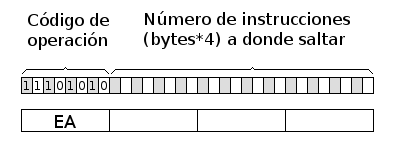
\includegraphics[width=14cm]{graphs/codsalto.png}
  \caption{Formato de instrucción de salto}
  \label{fig:codsalto}
\end{figure}

Los pasos para calcular la instrucción de salto serían.

\begin{itemize}
  \item Restar la dirección a saltar a la dirección actual
  \item Dividir entre 4
  \item Añadir {\tt 0xEA} al byte alto
\end{itemize}

Como todo son constantes en teoría podríamos implementar la
macro con dos instrucciones. Desgraciadamente el preprocesador
que usamos no es muy potente y si un operando es una etiqueta
sólo nos permite operar con sumas y restas. No podemos hacer las
divisiones o desplazamientos que necesitamos, con lo que emplearemos
una tercera instrucción para hacer el desplazamiento.

La dirección actual es {\tt \textbackslash vector}, la de la RTI
es {\tt \textbackslash dirRTI} y hay que restarle 8 por el
segmentado de la CPU.
\\
{\it instrucción }$ = (\textbackslash dirRTI-\textbackslash vector-8)/4 + 0xEA000000$ \\
{\it instrucción }$ = (\textbackslash dirRTI-\textbackslash vector)/4 + 0xE9FFFFFE$ \\
{\it instrucción }$ = (\textbackslash dirRTI-\textbackslash vector+3A7FFFFF8)/4$ \\
{\it instrucción }$ = (\textbackslash dirRTI-\textbackslash vector+A7FFFFFB) ROR 2$

Vemos cómo en el último paso hemos transformado una división en una rotación, donde los
2 bits menos significativos (ambos a 1) pasan a ser los más significativos tras la
rotación.

\section{Resultado}

El código final queda como sigue.

\begin{lstlisting}
      .macro    ADDEXC  vector, dirRTI
        ldr     r1, =(\dirRTI-\vector+0xa7fffffb)
        ROR     r1, #2
        str     r1, [r0, #\vector]
      .endm
\end{lstlisting}

Como la arquitectura no nos permite escribir en una dirección absoluta, antes
de invocar la macro debemos asegurarnos de que {\tt r0} apunte al vector de
interrupciones, es decir que valga {\tt 0}. En caso de usar esta macro como
primera instrucción del programa Bare Metal podemos omitir la inicialización
de {\tt r0}, ya que en las especificaciones de carga del {\tt kernel.img} se
establece este valor.

\chapterend


%%%%%%%%%%%%%%%%%%%%%%%%%%%%%%%%%%%%%%%%%%%%%%%%%%%%%%%%%%%%%%%%%%%
%%% Documento LaTeX                                             %%%
%%%%%%%%%%%%%%%%%%%%%%%%%%%%%%%%%%%%%%%%%%%%%%%%%%%%%%%%%%%%%%%%%%%
% Título:   Apéndice A
% Autor:    Ignacio Moreno Doblas
% Fecha:    2014-02-01
% Versión:  0.5.0
%%%%%%%%%%%%%%%%%%%%%%%%%%%%%%%%%%%%%%%%%%%%%%%%%%%%%%%%%%%%%%%%%%%%

\pagestyle{fancy}
\fancyhead[LE,RO]{\thepage}
\fancyhead[RE]{Apéndice} %
\fancyhead[LO]{\nouppercase{\rightmark}}
%\fancyhead[RE]{Parte \thepart \rightmark} %

\chapterbegin{Funcionamiento de la placa auxiliar}
\label{chp:PlacaAux}
\minitoc

\section{Esquema}

\begin{figure}[h]
  \centering
    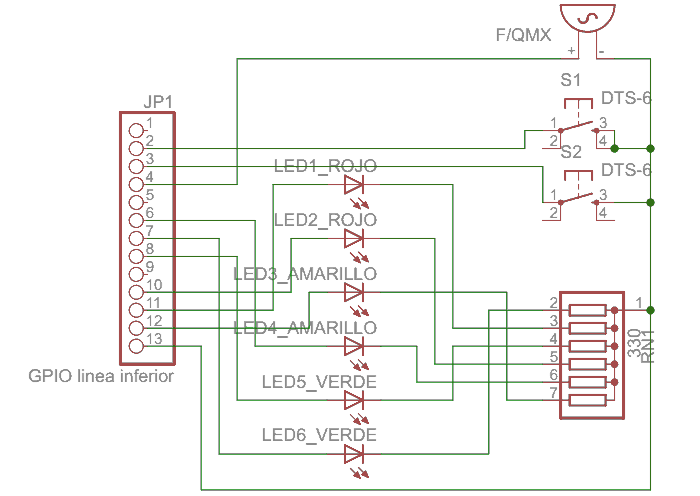
\includegraphics[width=14cm]{graphs/circuito.png}
  \caption{Esquema del circuito}
  \label{fig:circuito}
\end{figure}

Es un circuito sencillo y se puede montar en una protoboard sin
problemas, el esquema es el siguiente. Se conecta en la fila
inferior del conector GPIO, dejando libre la superior para el puerto
serie y otros propósitos.

\section{Pinout}

El puerto GPIO varía ligeramente dependiendo del modelo de Raspberry. En nuestro caso
la mayor diferencia está entre la revisión 1 y la 2, ya que el modelo B+ es compatible.
Al ser idénticos los primeros 26 pines, cualquier periférico diseñado para la revisión 2
es compatible con el modelo B+ (pero no al contrario).

La zona marcada con un recuadro verde es donde conectaremos nuestra placa auxiliar.

\begin{figure}[h]
  \centering
    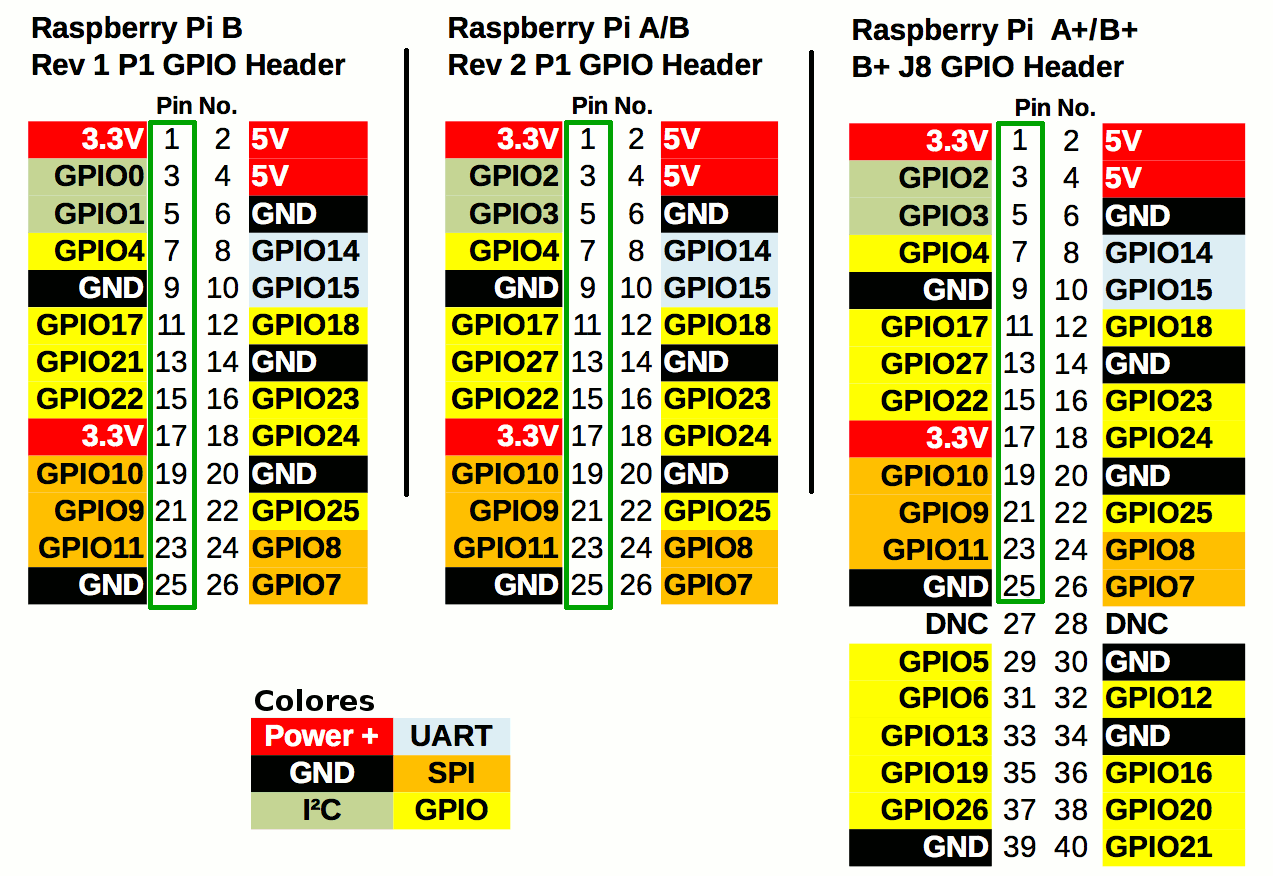
\includegraphics[width=14cm]{graphs/RaspberryGPIO.png}
  \caption{Pinout del puerto GPIO}
  \label{fig:pinout}
\end{figure}

\section{Correspondencia}

En la siguiente tabla vemos la correspondencia entre puertos del GPIO y
componentes. Los componentes son: 2 pulsadores, 6 LEDs y un altavoz
piezoeléctrico. Los números marcados con asterisco tienen otra
correspondencia en la revisión 1.

\begin{longtable}{ p{1.8cm} | p{1.2cm} | p{2cm} | p{5cm}}
\hline
{\bf Nombre} & {\bf GPIO} & {\bf Tipo} & {\bf Descripción} \\ \hline
LED1 & 9 & Salida & Diodo led color rojo \\ \hline
LED2 & 10 & Salida & Diodo led color rojo \\ \hline
LED3 & 11 & Salida & Diodo led color amarillo \\ \hline
LED4 & 17 & Salida & Diodo led color amarillo \\ \hline
LED5 & 22 & Salida & Diodo led color verde \\ \hline
LED6 & 27* & Salida & Diodo led color verde \\ \hline
BOT1 & 2* & Entrada & Pulsador izquierdo \\ \hline
BOT2 & 3* & Entrada & Pulsador derecho \\ \hline
ALT & 4 & Salida & Altavoz piezoeléctrico \\ \hline
\caption{Correspondencia entre pines y componentes}
\label{tab:berry}
\end{longtable}

\newpage

\section{Funcionamiento}

Los LEDs son salidas que se activan (encienden) cuando escribimos un 1
en el puerto correspondiente. Cuando están a 0 permanecen apagados. Podemos
jugar con los tiempos de encendido/apagado para simular intensidades de luz
intermedias.

El altavoz piezoeléctrico es otra salida, conectada al puerto GPIO 4. A diferencia
de los LEDs no basta un 0 ó un 1 para activarlo, necesitamos enviar una onda
cuadrada al altavoz para que éste suene. Es decir, hay que cambiar rápidamente de
0 a 1 y viceversa, además a una frecuencia que sea audible (entre 20 y 20000 Hz).

Por último tenemos los pulsadores. Eléctricamente son interruptores que conectan
el pin a masa cuando están presionados. Cuando están en reposo entran en juego
unas resistencias internas de la Raspberry (de pull-up) que anulan el comportamiento de
las de pull-up/pull-down que se cambian por software. De esta forma los pulsadores
envian un 0 lógico por el pin cuando están pulsados y un 1 cuando están en reposo.

Los pulsadores y el LED verde de la derecha se corresponden con
distintos puertos según el modelo de Raspberry. Podemos hacer que nuestro
programa sea compatible con todos los modelos, comprobando a la vez en las distintas
entradas en el caso de los pulsadores, o escribiendo a la vez en ambas salidas
en el caso del LED verde.

En la figura \ref{fig:pinout2} tenemos la correspondencia entre pines, componentes
y puertos GPIO.

\begin{figure}[h]
  \centering
    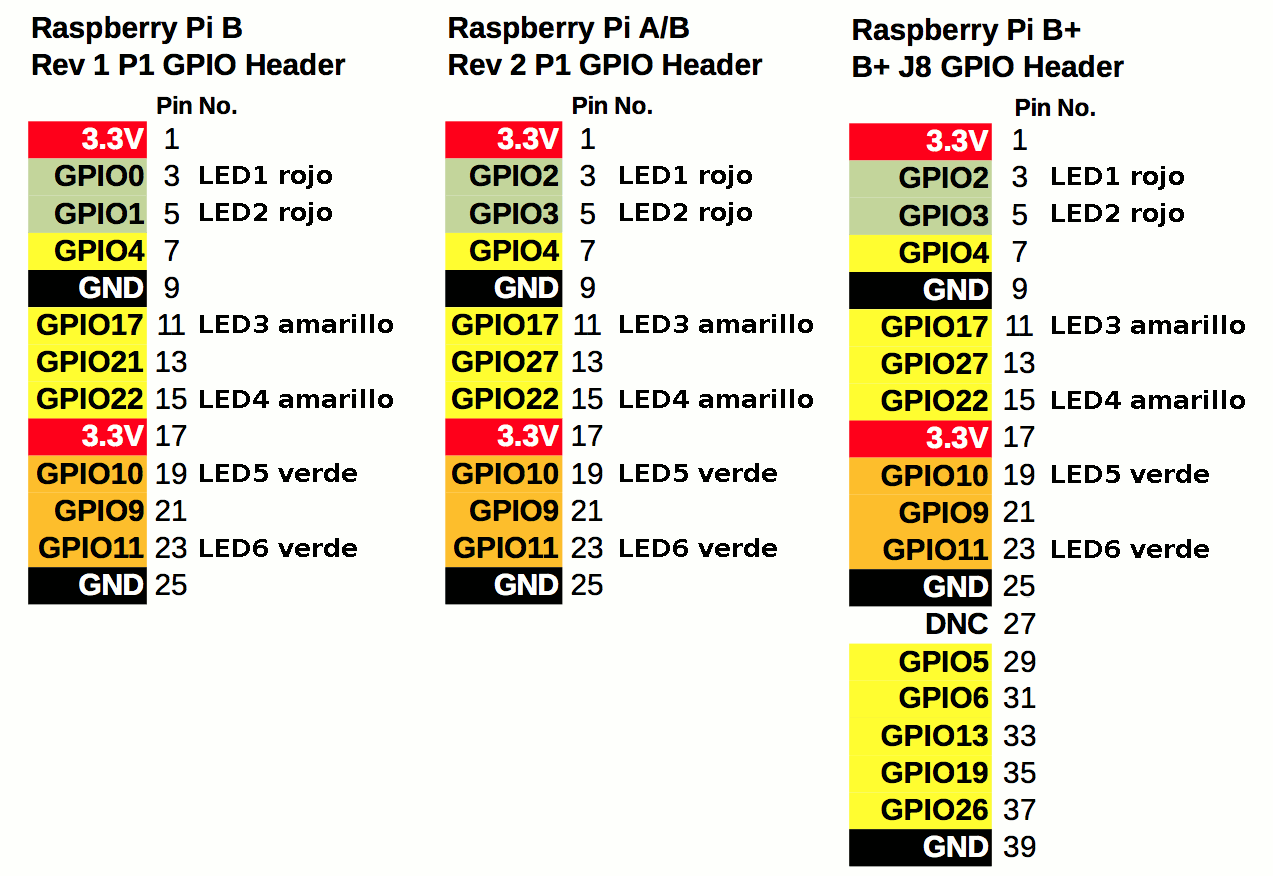
\includegraphics[width=14cm]{graphs/RaspberryGPIOaux.png}
  \caption{Correspondencia LEDs y GPIO}
  \label{fig:pinout2}
\end{figure}

\chapterend


\pagestyle{fancy}
\fancyhead[LE,RO]{\thepage}
\fancyhead[RE]{Apéndice} %
\fancyhead[LO]{\nouppercase{\rightmark}}
%\fancyhead[RE]{Parte \thepart \rightmark} %

\chapterbegin{Cable serie y bootloaders}
\label{chp:SerieBoot}
\minitoc

\section{Introducción}

En esta sección profundizamos sobre dos métodos para cargar programas en Bare Metal sin
necesidad de insertar y extraer continuamente la tarjeta SD. Existe un tercer método que
no explicamos aquí, el del cable JTAG, pero pueden consultar los archivos
README del repositorio de David Welch\cite{DWEL}.

Este apéndice está basado en el contenido de dicho repositorio, y el código fuente del
bootloader que mostramos aquí es idéntico, el cual reproducimos con permiso del autor.

\section{Cable USB-serie desde el ordenador de desarrollo}

Con esta opción hacemos todo el trabajo de ensamblado y enlazado en nuestro ordenador
de desarrollo, para luego transferir el archivo Bare Metal por el puerto serie
directamente a la Raspberry. Necesitamos un adaptador USB-serie como el de la siguiente
figura \ref{fig:mapamemoria}.

\begin{figure}[h]
  \centering
    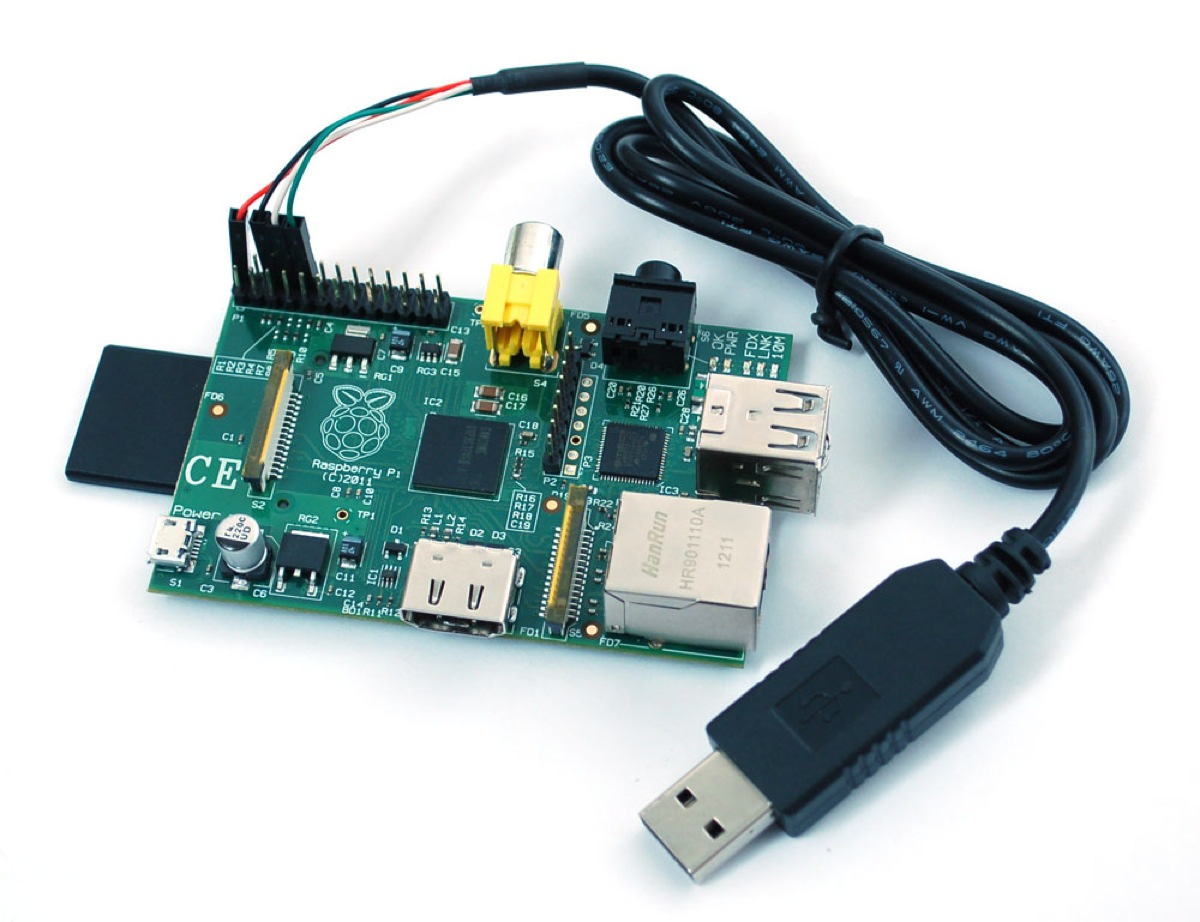
\includegraphics[width=14cm]{graphs/ARM_RaspberryPi_serial.jpg}
  \caption{Cable USB-serie}
  \label{fig:cableusb}
\end{figure}

Lo primero que tenemos que hacer es cargar el bootloader
\footnote{\url{https://github.com/dwelch67/raspberrypi/blob/master/bootloader05/kernel.img?raw=true}}
en la SD y alimentar la Raspberry. Es necesario resetear la Raspberry cada vez que
queramos cargar un programa Bare Metal nuevo, y esto se hace manualmente desenchufando y
enchufando la alimentación, o bien con el método automático que explicamos en la última sección.

Debemos conectar los 3 cables que van del adaptador USB-serie a la Raspberry, con los pines
tercero, cuarto y quinto de la fila superior del puerto GPIO. El tercer pin es la masa, en el
adaptador es un cable negro o marcado con GND en la serigrafía. El cuarto pin es GPIO 14 ó TXD,
que se corresponde con el pin RXD en el adaptador. Por último el quinto pin es GPIO 15 ó RXD y
va conectado al pin TXD del adaptador. Nótese que los cables están cruzados, el pin que
transmite desde el PC es el que recibe en la Raspberry y viceversa.

La primera vez que probemos el cable es recomendable probar con un programa simple como un
LED parpadeante, por ejemplo el último {\tt esbn5.s} del capítulo \ref{chp:Subrut}. A partir
del código fuente generamos el binario en Bare Metal, para lo cual necesitamos el toolchain
(cadena de herramientas) ARM, de la que usaremos el ensamblador {\tt as}, el enlazador {\tt ld}
y el copiador de secciones {\tt objcopy}. A estas herramientas, que generan binarios
o ejecutables para una plataforma diferente a la de la máquina que realiza la compilación,
se las denomina {\it herramientas de compilación cruzada}.

En estos momentos tenemos el binario Bare Metal generado, llamémoslo {\tt esbn5.img}. El
siguiente paso es enviar este archivo por el puerto serie de forma que se ejecute en la
Raspberry. Pero no lo enviamos de cualquier manera, sino que emplearemos un protocolo
de transferencia que se llama XMODEM. Por suerte es uno de los protocolos mejor soportados
por los emuladores de terminal.

Dependiendo de nuestra plataforma hay distintos emuladores de terminal disponibles. Para
Windows tenemos {\tt HyperTerminal} o {\tt Tera Term}, y en Linux tenemos {\tt minicom},
aunque para lo que queremos hacer (enviar un archivo) nos basta con el comando {\tt sx}.

Antes de nada hay que configurar los parámetros del puerto serie en el emulador de
terminal que estemos empleando. Los valores son: 8 bits de datos, sin paridad, 1 bit de
parada, sin flujo de control y velocidad de transferencia de 115200 baudios. Son todos
parámetros por defecto excepto la velocidad, por lo que hay que asegurarse de cambiar
la velocidad antes de proceder a transferir el archivo.

Luego elegimos el protocolo, {\tt XMODEM}, y le damos a transferir, seleccionando
nuestro {\tt esbn5.img} como archivo de origen. Si todo ha ido bien debería aparecer
un mensaje indicándolo en nuestro programa terminal y observaremos el LED parpadenado
en la Raspberry, prueba de que la transferencia ha sido exitosa.

En Linux es fácil automatizar este proceso con el comando {\tt sx}, que es creando
el siguiente script {\tt enviar}.

\begin{lstlisting}
stty -F /dev/ttyUSB0 115200
sx $1 < /dev/ttyUSB0 > /dev/ttyUSB0
\end{lstlisting}

Y para enviar el archivo anterior con este script escribimos bajo línea de comandos lo siguiente.

\begin{lstlisting}
./enviar esbn5.img
\end{lstlisting}

\section{Cable serie-serie que comunica dos Raspberries}

Esta configuración es ideal si queremos emplear una Raspberry como ordenador de desarrollo.
Aunque también está la alternativa de trabajar con un ordenador de desarrollo aparte conectado
a una de las Raspberries mediante {\tt ssh}. La ventaja de esta última alternativa es que podemos
compilar desde la Raspberry sin necesidad de tener instaladas las herramientas de compilación
cruzada en tu ordenador. Y otra ventaja es que no necesitas estar físicamente cerca de la
Raspberry ni tener enchufado el adaptador USB, te puedes conectar inalámbricamente a la Raspberry
mediante un router Wifi (con cable Ethernet entre el router y la Raspberry).

Lo primero es diferenciar las dos Raspberries. A una la llamamos Raspberry de desarrollo,
en la cual tendremos instalado Raspbian y es en la que trabajamos directamente (con teclado y
pantalla) o bien nos conectamos con ella mediante ssh. A la otra la llamamos Raspberry Bare
Metal, en la que sobreescribimos el kernel.img de la SD con el mismo bootloader de antes. Es
en esta Raspberry donde se ejecutan los programas Bare Metal que vamos a desarrollar y por tanto
donde enchufaremos nuestra placa auxiliar.

La conexión entre ambas Raspberries se hace uniendo ambas masas y cruzando los cables TXD
y RXD de cada puerto serie, como viene indicado en la figura \ref{fig:pitopi}.

\begin{figure}[h]
  \centering
    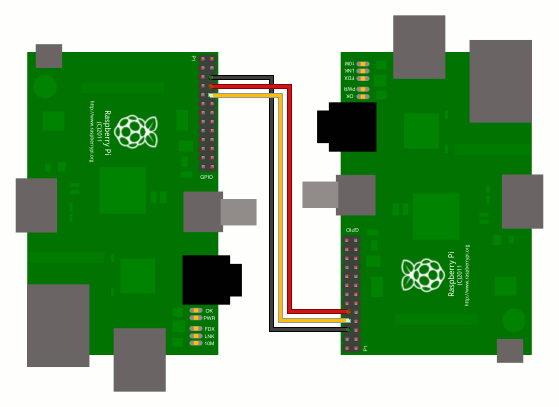
\includegraphics[width=14cm]{graphs/pitopi.png}
  \caption{Dos raspberries en serie cruzado}
  \label{fig:pitopi}
\end{figure}

Por defecto el puerto serie en Raspbian viene configurado como salida de consola. Esta
configuración no nos interesa, se usa para diagnosticar errores mostrando por un terminal
los mensajes del arranque. Pero nosotros queremos usarlo como un puerto serie genérico,
para lo cual es necesario hacer los siguientes cambios.

En el archivo {\tt /etc/inittab} descomentamos la línea que empieza con {\tt T0:23...} y
que hace mención a la cadena {\tt ttyAMA0}, y guardamos el archivo.

Luego en el archivo {\tt /boot/cmdline.txt} buscamos los dos sitios (puede haber uno sólo)
donde aparece {\tt ttyAMA0}. Borramos los textos que hay entre espacios y que incluyen el
{\tt ttyAMA0}, y después guardamos.

Para comprobar que todo ha ido bien reseteamos la Rasbperry con {\tt sudo reboot} y tras
el arranque escribimos.

\begin{lstlisting}
cat /proc/cmdline
\end{lstlisting}

Comprobando que efectivamente no hay se hace ninguna referencia a {\tt ttyAMA0}, y luego
escribimos este otro comando.

\begin{lstlisting}
ps aux | grep ttyAMA0
\end{lstlisting}

Para verificar que el único proceso que se lista en la salida es el del propio comando {\tt ps}
y no existen otros.

Llegados a este punto ya tenemos el puerto serie disponible para nosotros. El resto de pasos
serían como en el caso anterior, pero cambiando la referencia que se hace al puerto. Donde
antes aparecía {\tt /dev/ttyUSB0} (o algo similar) lo cambiamos por {\tt /dev/ttyAMA0}.

\section{Reseteo automático}

Resulta tedioso tener que desenchufar y enchufar la Raspberry cada vez que queremos introducir
un nuevo programa Bare Metal. Una solución intermedia es soldar los dos pines de Reset que
están serigrafiados como {\tt P6} en la Raspberry 2.0 o como {\tt RUN} en el modelo A+/B+.
A éstos pines le podemos conectar un pulsador, con simplificamos el reseteo, en lugar de
desenchufar y enchufar pulsamos un botón.

Sin embargo es muy conveniente buscar una solución totalmente automática, mediante la cual
el propio script que envía el archivo envíe una señal de Reset justo antes del envío. Para
evitar confusiones, en lugar de montar los dos pines del conector, montamos sólo uno, el
de la señal que provoca el Reset (el otro es la masa). Viene señalada con un círculo rojo
en la figura \ref{fig:pinReset}.

\begin{figure}[h]
  \centering
    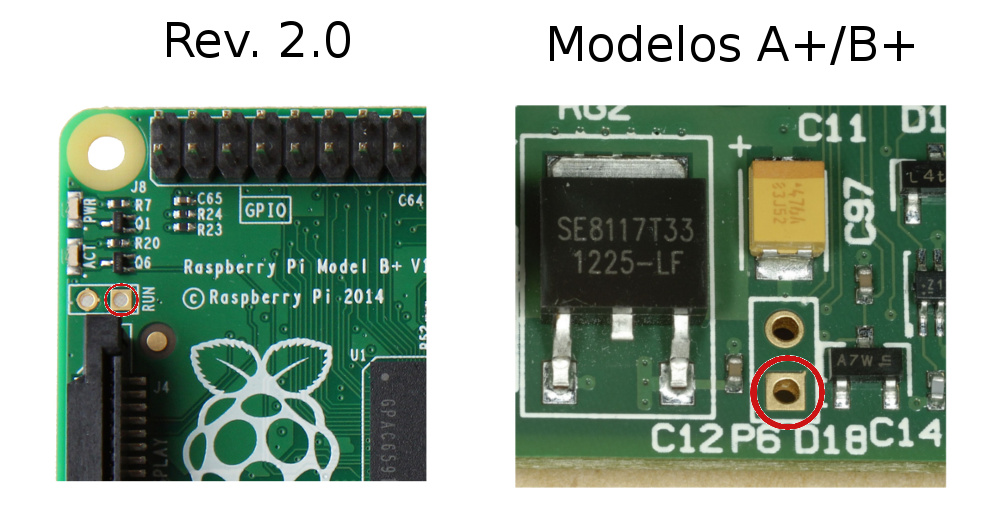
\includegraphics[width=14cm]{graphs/pinReset.jpg}
  \caption{Señal de Reset donde montar el pin}
  \label{fig:pinReset}
\end{figure}

De lo que se trata ahora es de enviar un pulso negativo a esa señal. En el caso del cable
USB-Serie lo haremos por una señal programable que no se emplea en el enlace serie llamada
{\tt DTR}. En el caso de conexión serie-serie entre dos Raspberries usaremos el pin GPIO 18
(justo a la derecha de RXD), valdría cualquier otro pin, pero por cercanía empleamos este.

Lo siguiente es hacer un programa que envíe dicho pulso en incluirlo en el script. Para
el cable USB-Serie empleamos este programa.

\begin{lstlisting}
int pulseDTR(int fd){
    int status;

    // leemos la señal de control status
    if (ioctl(fd, TIOCMGET, &status) == -1) {
        // manejamos el error
    }

    // Ponemos DTR a cero (activamos reset)
    status &= ~TIOCM_DTR;
    // y lo aplicamos a la señal de control
    if (ioctl(fd, TIOCMSET, &status) == -1) {
        // manejamos el error
    }
    // esperamos un poco
    usleep (400*1000);
    // Ahora ponemos DTR a uno (desactivamos reset)
    status |= TIOCM_DTR;
    // y lo aplicamos
    if (ioctl(fd, TIOCMSET, &status) == -1) {
        // manejamos el error
    }
    return 0;
}
\end{lstlisting}

En el caso de las dos Raspberries instalamos primero el paquete {\tt wiringPi}.

\begin{lstlisting}
git clone git://git.drogon.net/wiringPi
cd wiringPi
./build
\end{lstlisting}

E incluímos el pulso reset mediante comandos, por ejemplo nuestro script que compila
y envía el archivo (todo en un paso) quedaría así.

\begin{lstlisting}
gpio export 18 out
as -o tmp.o $1
gpio export 18 in
ld -e 0 -Ttext=0x8000 -o tmp.elf tmp.o
objcopy tmp.elf -O binary tmp.img
stty -F /dev/ttyAMA0 115200
sx tmp.img < /dev/ttyAMA0 > /dev/ttyAMA0
\end{lstlisting}

Observamos que el pulso de reset dura lo que tarde el programa en ensamblar, duración
más que suficiente como para provocar un Reset en la Raspberry Bare Metal. Para llamar
al script escribimos algo como esto.

\begin{lstlisting}
./compila esbn5.s
\end{lstlisting}

\section{Código fuente del bootloader}

Mostramos la parte principal del programa bootloader, el resto de archivos están
en el repositorio.

\begin{lstlisting}[caption={bootloader05.c},label={lst:bootloader}]
//-----------------------------------
unsigned char xstring[256];
//-----------------------------------
int notmain ( void )
{
    unsigned int ra;
    unsigned int rx;
    unsigned int addr;
    unsigned int block;
    unsigned int state;

    unsigned int crc;

    uart_init();
    hexstring(0x12345678);
    hexstring(GETPC());
    hexstring(ARMBASE);
    timer_init();

//SOH 0x01
//ACK 0x06
//NAK 0x15
//EOT 0x04

//block numbers start with 1

//132 byte packet
//starts with SOH
//block number byte
//255-block number
//128 bytes of data
//checksum byte (whole packet)
//a single EOT instead of SOH when done, send an ACK on it too

    block=1;
    addr=ARMBASE;
    state=0;
    crc=0;
    rx=timer_tick();
    while(1)
    {
        ra=timer_tick();
        if((ra-rx)>=4000000)
        {
            uart_send(0x15);
            rx+=4000000;
        }
        if((uart_lcr()&0x01)==0) continue;
        xstring[state]=uart_recv();
        rx=timer_tick();
        if(state==0)
        {
            if(xstring[state]==0x04)
            {
                uart_send(0x06);
                for(ra=0;ra<30;ra++) hexstring(ra);
                hexstring(0x11111111);
                hexstring(0x22222222);
                hexstring(0x33333333);
                uart_flush();
                BRANCHTO(ARMBASE);
                break;
            }
        }
        switch(state)
        {
            case 0:
            {
                if(xstring[state]==0x01)
                {
                    crc=xstring[state];
                    state++;
                }
                else
                {
                    //state=0;
                    uart_send(0x15);
                }
                break;
            }
            case 1:
            {
                if(xstring[state]==block)
                {
                    crc+=xstring[state];
                    state++;
                }
                else
                {
                    state=0;
                    uart_send(0x15);
                }
                break;
            }
            case 2:
            {
                if(xstring[state]==(0xFF-xstring[state-1]))
                {
                    crc+=xstring[state];
                    state++;
                }
                else
                {
                    uart_send(0x15);
                    state=0;
                }
                break;
            }
            case 131:
            {
                crc&=0xFF;
                if(xstring[state]==crc)
                {
                    for(ra=0;ra<128;ra++)
                    {
                        PUT8(addr++,xstring[ra+3]);
                    }
                    uart_send(0x06);
                    block=(block+1)&0xFF;
                }
                else
                {
                    uart_send(0x15);
                }
                state=0;
                break;
            }
            default:
            {
                crc+=xstring[state];
                state++;
                break;
            }
        }
    }
    return(0);
}
\end{lstlisting}

Al comienzo se envían tres cadenas en hexadecimal por el puerto (0x12345678, GETPC() y ARMBASE)
para indicar que el bootloader está listo para recibir. Esto lo podemos ver si empleamos un
programa terminal como {\tt minicom} para leer del puerto.

Después se inicializan algunas variables y nos metemos en el bucle principal. Se supone que el
primer byte que tenemos que recibir desde el host es {\tt SOH}, en hexadecimal es {\tt 0x01}.
Si pasado un tiempo no recibimos nada, enviamos un {\tt NAK} ({\tt 0x15}) para indicarle al host
que estamos vivos. En realidad este comando sirve para decirle al host que el paquete recibido
es erróneo, que nos lo envíe nuevamente.

El host enviará a la Raspberry el archivo en trozos de 128 bytes cada uno (rellenando el último
trozo con ceros hasta que ocupe 128 bytes) con este formato.

\begin{figure}[h]
  \centering
    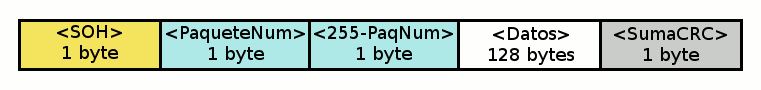
\includegraphics[width=14cm]{graphs/xmodem.png}
  \caption{Formato de paquete XMODEM}
  \label{fig:xmodem}
\end{figure}

Se trata del byte {\tt SOH} seguido del número de bloque, luego tenemos otra vez el número de
bloque pero complementado, a continuación los 128 bytes de datos para acabar con un último byte
de suma de comprobación. Este último byte es la suma de todos los anteriores, quedándonos con
los 8 bits menos significativos del resultado.

Entonces la Raspberry lleva la cuenta del byte por el que vamos dentro de dicho paquete a
partir de {\tt switch(state)}. De tal forma que si {\tt state} vale 0, lo que esperamos es
{\tt SOH} o {\tt EOT}, cualquier otro valor indica que algo va mal por tanto enviamos un
{\tt NAK} al host y ponemos {\tt state} a cero.

Para los estados 1 y 2 simplemente comprobamos que el byte recibido coincide con el número
de bloque, y reportamos error en caso contrario de la misma forma que antes (enviando
{\tt NAK} y {\tt state=0}).

Luego tenemos los estados que van entre 3 y 131, en los que vamos escribiendo el fichero en
memoria e incrementando el puntero, a la vez que vamos calculando el byte de suma para
la comprobación.

Por último tenemos el estado 131, en el cual ya hemos recibido los bytes de datos y lo que
leemos ahora es el byte de suma de comprobación. Comparamos que coincide con el valor esperado,
respondiendo con {\tt ACK}, o notificamos del error como siempre (con {\tt NAK} y {\tt state=0}).

En cuanto el host recibe el {\tt ACK} del último paquete enviado, éste en lugar de enviar
de nuevo un paquete completo, envía un sólo byte, {\tt EOT}, para indicar a la Raspberry
que ya no quedan más paquetes por enviar y se acaba la transmisión.

Esta situación la comprueba la Raspberry al principio de cada paquete, de tal forma que si
recimibos un {\tt EOT} del host damos por acabada la transmisión y ejecutamos el archivo
Bare Metal leído con {\tt BRANCHTO}, que en bajo nivel se corresponde con saltar a {\tt 0x8000}.

En la figura \ref{fig:transm} tenemos un ejemplo completo de transmisión. En él se envían 4
paquetes, con errores y reenvíos en los paquetes 2 y 3. Podría tratarse de un archivo que
ocupase 500 bytes, y que la utilidad {\tt sx} haya rellenado en el último paquete 12 bytes
con ceros, para que de esta forma todos los paquetes ocupen 128 bytes (la parte útil, contando
cabeceras y demás cada paquete ocupa 132 bytes).

\begin{figure}[h]
  \centering
    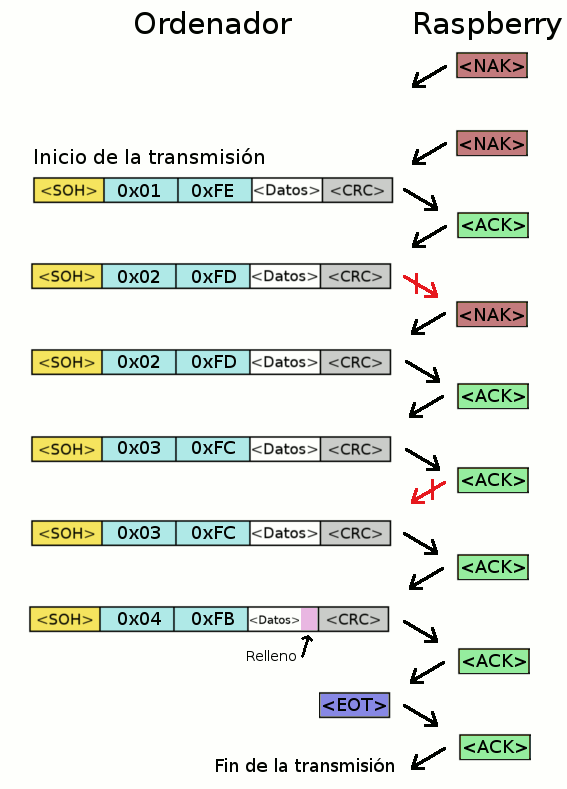
\includegraphics[width=14cm]{graphs/transm.png}
  \caption{Ejemplo de transmisión}
  \label{fig:transm}
\end{figure}

\chapterend


\pagestyle{fancy}
\fancyhead[LE,RO]{\thepage}
\fancyhead[RE]{Apéndice} %
\fancyhead[LO]{\nouppercase{\rightmark}}
%\fancyhead[RE]{Parte \thepart \rightmark} %

\chapterbegin{Resistencias programables de pull-up y pull-down}
\label{chp:resistencias}
\minitoc

\section{Introducción}

En general las resistencias de pull-up y pull-down son resistencias que se ponen en
las entradas para fijar la tensión que de otra forma quedaría indeterminada, al estar
en situación de circuito abierto o alta impedancia. El ejemplo típico donde se usa es
en un pulsador. Eléctricamente un pulsador no es más que un interruptor que deja pasar
la corriente cuando está pulsado y se queda en circuito abierto en su posición de reposo
(sin pulsar). De los dos contactos que tiene, uno se conecta a masa y el otro al pin de
entrada de la Raspberry. Así que cuando lo pulsamos hacemos un corto que llevaría los cero
voltios de la masa al pin de entrada (enviamos un cero lógico), pero cuando está sin pulsar
no enviamos nada al pin, éste se queda en lo que se denomina alta impedancia.

Todos los pines del GPIO en la Raspberry se pueden configurar por software para que
se comporten como queramos: o bien sin resistencia, o con una resistencia a Vcc (pull-up) o
con una resistencia a masa (pull-down). Este tipo de resistencias son débiles (weak) debido
a que están dentro de la pastilla (SoC) y se implementan con transistores. Se puede
anular el efecto de estas resistencias poniendo resistencias externas.

\section{Pulsadores en la placa auxiliar}

En la placa auxiliar tenemos dos pulsadores conectados a GPIO 2 y GPIO 3. No es casualidad
que estén conectados concretamente a esos dos pines. Son los únicos pines que tienen
resistencias externas de pull-up, concretamente de 1K8, que anulan cualquier configuración
interna que pongamos. La razón es porque las resistencias internas son débiles, tienen un
valor aproximado de unos 50K. Cuando hay dos resistencias en paralelo como es el caso,
la de menor valor anula el efecto de la de mayor valor.

Por tanto si configuramos GPIO 2 ó GPIO 3 como entradas, independientemente del valor
que configuremos por software, se comportarán siempre como si sólo tuviesen una
resistencia de pull-up.

El propósito de este apéndice es aprender a cambiar la configuración de los pull-ups/pull-downs
en caso de usar otras placas auxiliares distintas. En la nuestra las únicas entradas (pulsadores)
que hay están resueltas con las resistencias antes comentadas que tiene la Raspberry sólo en
esos dos pines.

\section{Ejemplo de aplicación}

El montaje que proponemos es con uno de los pines de la fila superior, en concreto el
pin GPIO 18 que hay a la derecha de los pines del puerto serie. En estos ejemplos
no vamos a requerir la placa auxiliar, de esta forma
dejamos libres los pines Vcc (3.3V), ya que necesitaremos uno para el último ejemplo. 

\subsection{Pulsador a masa sin cambiar configuración}

En este primer ejemplo vamos a tratar de encender el LED interno de la Raspberry llamado
ACT (OK) mediante un pulsador externo. El primer montaje sería el de
la figura.

El esquema sería el de la figura \ref{fig:circuito1}.

\begin{figure}[h]
  \centering
    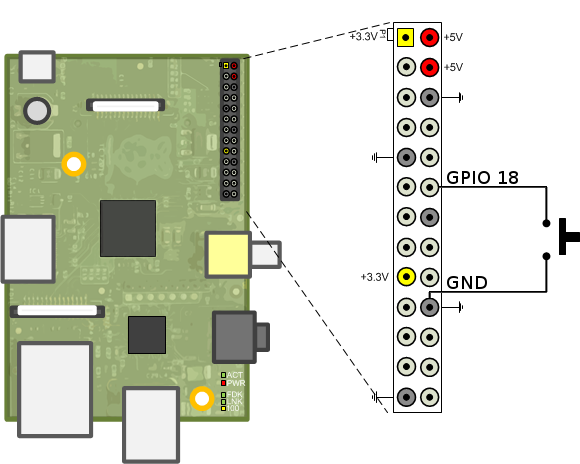
\includegraphics[width=14cm]{graphs/circuito1.png}
  \caption{Pulsador a masa}
  \label{fig:circuito1}
\end{figure}

Ahora escribimos el código. Como el pin GPIO que controla dicho LED es distinto en los
modelos normales que en los A+/B+, enviamos la señal a ambos pines. En el modelo normal
sería GPIO 16 y en el plus, el GPIO 47.

\begin{lstlisting}[caption={apend1.s},label={lst:codigoApendice_1}]
        .include  "inter.inc"
.text
        ldr     r0, =GPBASE
/* guia bits           xx999888777666555444333222111000*/
        mov     r1, #0b00000000000001000000000000000000
        str     r1, [r0, #GPFSEL1]
/* guia bits           xx999888777666555444333222111000*/
        mov     r1, #0b00000000001000000000000000000000
        str     r1, [r0, #GPFSEL4]
/* guia bits           10987654321098765432109876543210*/
        mov     r2, #0b00000000000000010000000000000000
/* guia bits           32109876543210987654321098765432*/
        mov     r3, #0b00000000000000001000000000000000
bucle:  str     r2, [r0, #GPCLR0]   @ apago GPIO 16
        str     r3, [r0, #GPCLR1]   @ apago GPIO 47
        ldr     r1, [r0, #GPLEV0]
/* guia bits           10987654321098765432109876543210*/
        tst     r1, #0b00000000000001000000000000000100
        streq   r2, [r0, #GPSET0]   @ enciendo GPIO 16
        streq   r3, [r0, #GPSET1]   @ enciendo GPIO 47
        b       bucle
\end{lstlisting}

Probamos el código y comprobamos que al pulsar el botón izquierdo no pasa nada,
el LED está siempre encendido.

Esto se debe a que por defecto el pin GPIO 18 está configurando con una resistencia de
pull-down y nosotros necesitamos una de pull-up, de lo contrario siempre leeremos un cero
por dicho pin. Los valores por defecto (tras el reset) se pueden consultar en la página
103 del datasheet, aunque la mayor parte de los pines disponibles por el puerto estan
a pull-down.

Para solventar ésto hay tres opciones: o conectar el otro terminal del interruptor a Vcc en
lugar de a GND, o configurar el pin para cambiarlo de pull-down a pull-up, o conectar una
resistencia externa a Vcc que anule el pull-down interno. Nosotros vamos a explorar las dos
primeras opciones.

\subsection{Pulsador a masa cambiando configuración}

En este ejemplo vamos a configurar GPIO 18 a pull-up de acuerdo a la siguiente
figura \ref{fig:pullup}.

\begin{figure}[h]
  \centering
    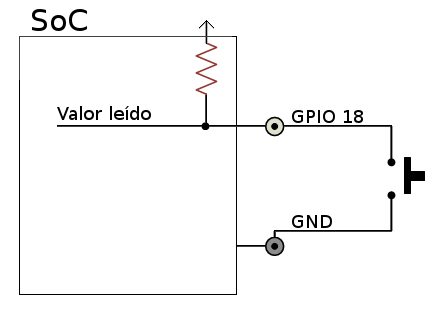
\includegraphics[width=14cm]{graphs/pullup.png}
  \caption{Resistencia interna de pull-up}
  \label{fig:pullup}
\end{figure}

Para configurar un pin determinado en pull-up/pull-down/desconectado seguimos los
siguientes pasos.

\begin{enumerate}
  \item Escribir en {\tt GPPUD} el tipo de resistencia que queremos. Un 0 sería
si no queremos resistencia, un 1 si es de pull-down ó un 2 si lo que queremos es un
pull-ups.
  \item Esperar 150 ciclos. Esto provee el tiempo requerido de {\tt set-up} para controlar la señal.
  \item Escribir en {\tt GPPUDCLK0/1} un 1 en la posición de los pines que queramos modificar,
mientras que los que estén a 0 mantendrán su antiguo estado.
  \item Esperar otros 150 ciclos. Con esto le damos tiempo de {\tt hold} suficiente a la señal.
  \item Poner GPPUD en su estado de reposo, que sería a valor 0 (desactivado).
  \item Escribir un 0 en {\tt GPPUDCLK0/1}.
\end{enumerate}

Una de las cosas que tenemos que hacer es esperar 150 ciclos (como mínimo). Como
sabemos que un salto condicional tarda al menos dos ciclos en ejecutarse, nuestra rutina
de retardo sería la siguiente.

\begin{lstlisting}
wait:   mov     r1, #50
wait1:  subs    r1, #1
        bne     wait1
        bx      lr
\end{lstlisting}

Y el código que hace todo lo anterior, para poner a pull-up el GPIO 18 (donde hemos puesto
el pulsador) es el siguiente.

\begin{lstlisting}
        str     r1, [r0, #GPPUD]
        bl      wait
/* guia bits           10987654321098765432109876543210*/
        mov     r1, #0b00000000000001000000000000000100
        str     r1, [r0, #GPPUDCLK0]
        bl      wait
        mov     r1, #0
        str     r1, [r0, #GPPUD]
        str     r1, [r0, #GPPUDCLK0]
\end{lstlisting}

El ejemplo completo quedaría así.

\begin{lstlisting}[caption={apend2.s},label={lst:codigoApendice_2}]
        .include  "inter.inc"
.text
        ldr     r0, =GPBASE
/* guia bits           xx999888777666555444333222111000*/
        mov     r1, #0b00000000000001000000000000000000
        str     r1, [r0, #GPFSEL1]
/* guia bits           xx999888777666555444333222111000*/
        mov     r1, #0b00000000001000000000000000000000
        str     r1, [r0, #GPFSEL4]
        mov     r1, #2
        str     r1, [r0, #GPPUD]
        bl      wait
/* guia bits           10987654321098765432109876543210*/
        mov     r1, #0b00000000000001000000000000000100
        str     r1, [r0, #GPPUDCLK0]
        bl      wait
        mov     r1, #0
        str     r1, [r0, #GPPUD]
        str     r1, [r0, #GPPUDCLK0]
/* guia bits           10987654321098765432109876543210*/
        mov     r2, #0b00000000000000010000000000000000
/* guia bits           32109876543210987654321098765432*/
        mov     r3, #0b00000000000000001000000000000000
bucle:  str     r2, [r0, #GPCLR0]   @ apago GPIO 16
        str     r3, [r0, #GPCLR1]   @ apago GPIO 47
        ldr     r1, [r0, #GPLEV0]
/* guia bits           10987654321098765432109876543210*/
        tst     r1, #0b00000000000001000000000000000100
        streq   r2, [r0, #GPSET0]   @ enciendo GPIO 16
        streq   r3, [r0, #GPSET1]   @ enciendo GPIO 47
        b       bucle

wait:   mov     r1, #50
wait1:  subs    r1, #1
        bne     wait1
        bx      lr
\end{lstlisting}

Comprobamos cómo ahora sí funciona, y mientras tenemos el botón presionado,
el LED se enciende, apagándose en cuanto lo soltamos.

\subsection{Pulsador a Vcc sin cambiar configuración}

Cambiamos es montaje, y en lugar de a GND conectamos el pulsador a Vcc según
la figura \ref{fig:circuito2}.

\begin{figure}[h]
  \centering
    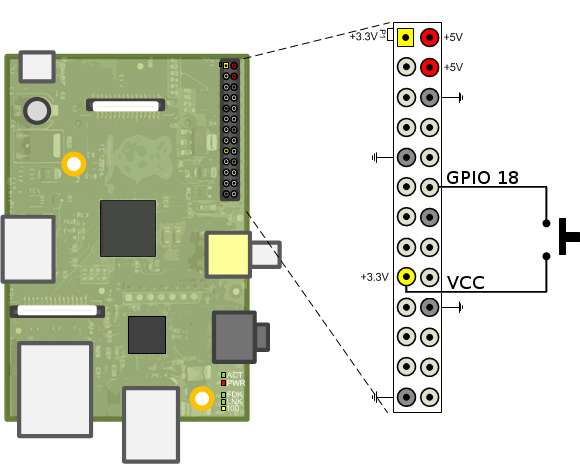
\includegraphics[width=14cm]{graphs/circuito2.png}
  \caption{Pulsador a Vcc}
  \label{fig:circuito2}
\end{figure}

De esta forma aprovechamos que ese pin en concreto está conectado a pull-down tras
el reset, por lo que no habría que cambiar la configuración del pin para obtener
lo que vemos en la figura \ref{fig:pulldown}.

Prácticamente tendríamos el mismo código que en {\tt apend1.s} no nos funcionaba,
la única diferencia es que cambiamos los {\tt streq} por {\tt strne}.

\begin{lstlisting}[caption={apend3.s},label={lst:codigoApendice_3}]
        .include  "inter.inc"
.text
        ldr     r0, =GPBASE
/* guia bits           xx999888777666555444333222111000*/
        mov     r1, #0b00000000000001000000000000000000
        str     r1, [r0, #GPFSEL1]
/* guia bits           xx999888777666555444333222111000*/
        mov     r1, #0b00000000001000000000000000000000
        str     r1, [r0, #GPFSEL4]
/* guia bits           10987654321098765432109876543210*/
        mov     r2, #0b00000000000000010000000000000000
/* guia bits           32109876543210987654321098765432*/
        mov     r3, #0b00000000000000001000000000000000
bucle:  str     r2, [r0, #GPCLR0]   @ apago GPIO 16
        str     r3, [r0, #GPCLR1]   @ apago GPIO 47
        ldr     r1, [r0, #GPLEV0]
/* guia bits           10987654321098765432109876543210*/
        tst     r1, #0b00000000000001000000000000000100
        strne   r2, [r0, #GPSET0]   @ enciendo GPIO 16
        strne   r3, [r0, #GPSET1]   @ enciendo GPIO 47
        b       bucle
\end{lstlisting}

\begin{figure}[h]
  \centering
    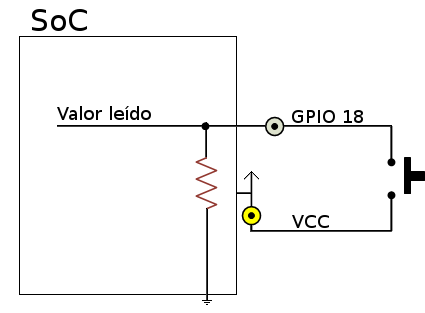
\includegraphics[width=14cm]{graphs/pulldown.png}
  \caption{Resistencia interna de pull-down}
  \label{fig:pulldown}
\end{figure}

\chapterend


% Formato de documento en la parte final.
\backmatter
%Hace que los capítulos y títulos nivel inferior no aparezcan numerados (lo que es ideal para conclusiones o notas finales).

% Bibliografía
% Encabezamiento %
\pagestyle{fancy}
\fancyhead[LE,RO]{\thepage}
\fancyhead[LO]{Bibliografía}
%\fancyhead[RE]{Parte \thepart \rightmark} %
\fancyhead[RE]{\nouppercase{\rightmark}} %

%Inclusión de bibliografía%
\bibliography{E2.Bibliografia} %Úsese el nombre del fichero sin extensión

%Inclusión en el índice (Tabla de contenidos)
\addcontentsline{toc}{chapter}{Bibliografía}

%Formateo de estilo de bibliografía
% Otros formatos: plain, unsrt, abbrv
%  plain: las entradas se ordenan alfabéticamente y se etiquetan con un número (p.ej., [1])
% unsrt: igual que plain, pero aparecen en orden de citación.
% alpha: el etiquetado se hace por autor y año de publicación (p.ej., [Knu66]).
% abbrv: igual que alpha, pero más abreviado.
\bibliographystyle{unsrt}

%Impresión de todas las entradas bibliográficas
\nocite{*}

\chapterend


% Índice alfabético%
%%%%%%%%%%%%%%%%%%%%%%%%%%%%%%%%%%%%%%%%%%%%%%%%%%%%%%%%%%%%%%%%%%%
%%% Documento LaTeX                                             %%%
%%%%%%%%%%%%%%%%%%%%%%%%%%%%%%%%%%%%%%%%%%%%%%%%%%%%%%%%%%%%%%%%%%%
% Título:   Glosario (index)
% Autor:    Ignacio Moreno Doblas
% Fecha:    2014-02-01
% Versión:  0.5.0
%%%%%%%%%%%%%%%%%%%%%%%%%%%%%%%%%%%%%%%%%%%%%%%%%%%%%%%%%%%%%%%%%%%%

\pagestyle{fancy}
\fancyhead[LE,RO]{\thepage}
\fancyhead[LO]{Índice Alfabético}
%\fancyhead[RE]{Parte \thepart \rightmark} %
\fancyhead[RE]{\nouppercase{\rightmark}} %

%index of contents
\phantomsection
\addcontentsline{toc}{chapter}{Índice alfabético}
\printindex


%Example  Index Entry   Comment
%\index{hello}  hello, 1  Plain entry
%\index{hello!Peter}    Peter, 3  Subentry under 'hello'
%\index{Sam@\textsl{Sam}}   Sam, 2  Formatted entry
%\index{Lin@\textbf{Lin}}   Lin, 7  Same as above
%\index{Jenny|textbf}   Jenny, 3  Formatted page number
%\index{Joe|textit}   Joe, 5  Same as above
%\index{ecole@\'ecole}  école, 4  Handling of accents
%\index{Peter|see{hello}}   Peter, see hello  Cross-references
%\index{Jen|seealso{Jenny}}   Jen, see also Jenny   Same as above

\chapterend


\end{document}
